%%%%%%%%%%%%%%%%%%%%%%%%%%%%%%%%%%%%%%%%%%%%%%%%%%%%%%%%%%%%%%%%%%%%%%%%%%%%%
%%%
%%% File: utthesis2.doc, version 2.0jab, February 2002
%%%
%%% Based on: utthesis.doc, version 2.0, January 1995
%%% =============================================
%%% Copyright (c) 1995 by Dinesh Das.  All rights reserved.
%%% This file is free and can be modified or distributed as long as
%%% you meet the following conditions:
%%%
%%% (1) This copyright notice is kept intact on all modified copies.
%%% (2) If you modify this file, you MUST NOT use the original file name.
%%%
%%% This file contains a template that can be used with the package
%%% utthesis.sty and LaTeX2e to produce a thesis that meets the requirements
%%% of the Graduate School of The University of Texas at Austin.
%%%
%%% All of the commands defined by utthesis.sty have default values (see
%%% the file utthesis.sty for these values).  Thus, theoretically, you
%%% don't need to define values for any of them; you can run this file
%%% through LaTeX2e and produce an acceptable thesis, without any text.
%%% However, you probably want to set at least some of the macros (like
%%% \thesisauthor).  In that case, replace "..." with appropriate values,
%%% and uncomment the line (by removing the leading %'s).
%%%
%%%%%%%%%%%%%%%%%%%%%%%%%%%%%%%%%%%%%%%%%%%%%%%%%%%%%%%%%%%%%%%%%%%%%%%%%%%%%

%%%%%%%%%%%%%%%%%%%%%%%%%%%%%%%%%%%%%%%%%%%%%%%%%%%%%%%%%%%%%%%%%%%%%%%%%%%%%
%%%
%%
%% This file, and the corresponding tcdthesis.sty the accompanied it, have
%% been modified for the M.Sc. styles used in Trinity College, Dublin
%%
%%
%%%%%%%%%%%%%%%%%%%%%%%%%%%%%%%%%%%%%%%%%%%%%%%%%%%%%%%%%%%%%%%%%%%%%%%%%%%%%
\documentclass[a4paper, 12pt, oneside]{report}         %% LaTeX2e document.
\usepackage {tcdthesis}              %% Preamble.
\usepackage {bookmark}

\usepackage{graphicx,color}
\usepackage{tabularx}
\usepackage{array}
\usepackage{anysize}
\usepackage{amsmath}
\usepackage[square,numbers,sort&compress]{natbib} 
\usepackage{caption}
\usepackage{hyperref}
\usepackage{listings}
\usepackage{float}
\usepackage{tabularx}  
\usepackage{fancyvrb}
\usepackage{fancyhdr}
\usepackage{xcolor}
\usepackage{tikz}
\usetikzlibrary{arrows.meta} % For -Stealth arrowheads
\usepackage{pgfgantt}


\mastersthesis                       %% Uncomment one of these; if you don't
% \phdthesis                         %% use either, the default is \phdthesis.

%\thesisdraft                         %% Uncomment this if you want a draft
                                     %% version; this will print a timestamp
                                     %% on each page of your thesis.


\leftchapter                         %% Uncomment one of these if you want
% \centerchapter                     %% left-justified, centered or
% \rightchapter                      %% right-justified chapter headings.
                                     %% Chapter headings includes the
                                     %% Contents, Acknowledgments, Lists
                                     %% of Tables and Figures and the Vita.
                                     %% The default is \centerchapter.

% \singlespace                       %% Uncomment one of these if you want
\oneandhalfspace                     %% single-spacing, space-and-a-half
% \doublespace                       %% or double-spacing; the default is
                                     %% \oneandhalfspace, which is the
                                     %% minimum spacing accepted by the
                                     %% Graduate School.
                                     
\renewcommand{\thesisauthor}{Sibin George}                %% Your official TCD name.
\renewcommand{\thesismonth}{August}                    %% Month of submission of the document.
\renewcommand{\thesisyear}{2025}                      %% Year of submission of the document.
\renewcommand{\thesistitle}{Stream-Level Routing over QUIC: A WebTransport Proxy Architecture for Kubernetes}   %% The title of your dissertation; use mixed-case.
\renewcommand{\thesisauthorpreviousdegrees}{, Msc}    %% Your previous degrees, abbreviated; separate multiple degrees by commas.
\renewcommand{\thesissupervisor}{Dr. Stefan Weber}            %% Your thesis supervisor; use mixed-case and don't use any titles or degrees.
% \renewcommand{\thesiscosupervisor}{}                %% Your PhD. thesis co-supervisor; if any.

% \renewcommand{\thesiscommitteemembera}{}
% \renewcommand{\thesiscommitteememberb}{}
% \renewcommand{\thesiscommitteememberc}{}
% \renewcommand{\thesiscommitteememberd}{}
% \renewcommand{\thesiscommitteemembere}{}
% \renewcommand{\thesiscommitteememberf}{}
% \renewcommand{\thesiscommitteememberg}{}
% \renewcommand{\thesiscommitteememberh}{}
% \renewcommand{\thesiscommitteememberi}{}


\renewcommand{\thesisauthoraddress}{...}

\renewcommand{\thesisdedication}{...}     %% Your dedication, if you have one; use "\\" for linebreaks.


%%%%%%%%%%%%%%%%%%%%%%%%%%%%%%%%%%%%%%%%%%%%%%%%%%%%%%%%%%%%%%%%%%%%%%%%%%%%%
%%%
%%% The following commands are all optional, but useful if your requirements
%%% are different from the default values in tcdthesis.sty.  To use them,
%%% simply uncomment (remove the leading %) the line(s).

\renewcommand{\thesisdegree}{Master of Science in Computer Science}
                                     %% default is "DOCTOR OF PHILOSOPHY"
                                     %% for \phdthesis or "MASTER OF ARTS"
                                     %% for \mastersthesis.  Provide the
                                     %% correct FULL OFFICIAL name of
                                     %% the degree.
\renewcommand{\thesisdegreestream}{}
%%\renewcommand{\thesisdegreestream}{(Future Networks)}
                                     %% Default is empty. This is used on
                                     %% the title page of the thesis.

\renewcommand{\thesisdegreeabbreviation}{M.Sc.}
                                     %% Use this if you also use the above
                                     %% command; provide the OFFICIAL
                                     %% abbreviation of your thesis degree.
\renewcommand{\thesistype}{Dissertation}    %% Use this ONLY if your thesis type
                                     %% is NOT "Thesis" for \phdthesis
                                     %% or \mastersthesis.
                                     %% Provide the OFFICIAL type of the
                                     %% thesis; use mixed-case.

%%%
%%%%%%%%%%%%%%%%%%%%%%%%%%%%%%%%%%%%%%%%%%%%%%%%%%%%%%%%%%%%%%%%%%%%%%%%%%%%%


%% Settings for the listings package
\lstset{% setup parameters for listings:
  columns=fullflexible,  % avoids addition of extra spaces in unexpected positions
  keepspaces,            % causes alignment-by-spaces to be preserved in output
  basicstyle=\ttfamily,  % With fullflexible and keepspaces, using a non-monospaced
                         % font causes incorrect alignment of plain-text columns.
  backgroundcolor=\color{gray!10},
  keywordstyle=\bfseries\color{black!90},
  showstringspaces=false,
  numbers=none, numberstyle=\small\sffamily, stepnumber=0, numbersep=5pt}

%%------------------------------------------------
%% Listing macros
%%------------------------------------------------
%%
%% includecode:
%% \includecode{caption for table of listings}{caption for reader}{filename}
%% - includes a file with code and adds a caption that should describe the code in some detail and a shorter caption for the table of listings
\newcommand{\includecode}[4]{\lstinputlisting[floatplacement=H, caption={[#1]#2}, captionpos=b, frame=single, label={#3}]{#4}}
%%
%%------------------------------------------------
%% Image macros
%%------------------------------------------------
%%
%% includescalefigure:
%% \includescalefigure{label}{short caption}{long caption}{scale}{filename}
%% - includes a figure with a given label, a short caption for the table of contents and a longer caption that describes the figure in some detail and a scale factor 'scale'
\newcommand{\includescalefigure}[5]{
\begin{figure}[htb]
\centering
\includegraphics[width=#4\linewidth]{#5}
\captionsetup{width=.8\linewidth} 
\caption[#2]{#3}
\label{#1}
\end{figure}
}
%%
%% includefigure:
%% \includefigure{label}{short caption}{long caption}{filename}
%% - includes a figure with a given label, a short caption for the table of contents and a longer caption that describes the figure in some detail
\newcommand{\includefigure}[4]{
\begin{figure}[htb]
\centering
\includegraphics{#4}
\captionsetup{width=.8\linewidth} 
\caption[#2]{#3}
\label{#1}
\end{figure}
}


\begin{document}                                  %% BEGIN THE DOCUMENT

\thesistitlepage                                  %% Generate the title page.
\setcounter{secnumdepth}{4}
\setcounter{tocdepth}{4}

%\hypersetup{pageanchor=false}
%\thesisdeclarationpage                            %% Generate the declaration page.

%\thesispermissionpage                             %% Generate the copyright permission page
%\hypersetup{pageanchor=true}

\begin{thesisabstract}                            %% the abstract for your thesis
Modern web applications increasingly demand ultra-low-latency, multiplexed, and secure transport between browsers and cloud-native back-ends. While the QUIC transport protocol \cite{rfc9000} and its application-layer companion HTTP/3 \cite{rfc9114} eliminate head-of-line blocking and reduce handshake latency, current Kubernetes ingress controllers and reverse proxies only provide coarse-grained, connection-level load balancing. They terminate QUIC early and forward traffic over HTTP/1.1, losing the ability to route or observe individual WebTransport streams—a limitation that severely hampers real-time use cases such as interactive video, gaming, and telemetry.

This dissertation presents Custom Router Proxy, a novel WebTransport-aware proxy that operates natively inside Kubernetes \cite{kubernetes-docs}. By extending the Aioquic library \cite{aioquic-repo}, the custom router intercepts incoming QUIC packets, demultiplexes WebTransport streams containing audio, video, chat, or file data, and forwards each stream—via configuration-driven rules—to dedicated micro-services that publish processed results into Apache Pulsar topics \cite{pulsar-helm-repo}. The architecture leverages a 32-byte application header embedded in each stream to enable content-based routing at line rate while preserving end-to-end encryption.

Evaluation on a single-node Minikube cluster \cite{minikube-docs} demonstrates that the Router sustains sub-millisecond latency, linear throughput scaling up to five concurrent clients, and zero packet loss even under 90\% fragmentation. The system is fully declarative: routing rules and broker endpoints are supplied through Kubernetes ConfigMaps that support hot-reloading without service restarts. These results validate the feasibility of stream-level, QUIC-native ingress and establish a reusable foundation for deploying next-generation, real-time applications on Kubernetes.
\end{thesisabstract}

%\thesisdedicationpage                            %% Generate the dedication page.

\begin{thesisacknowledgments}                     %% Use this to write your
  Firstly, I would like to take this opportunity to thank my supervisor, Prof. Stefan Weber, for providing me with the right guidance as I navigated and explored this vast domain. I thank you again for sparking my curiosity during each meeting we had. To my parents and elder sister, thank you for the love and support from afar; your quiet encouragement and belief in me were a constant source of strength that carried me through this master’s journey.         %% acknowledgments; it can be anything
\end{thesisacknowledgments}                       %% allowed in LaTeX2e par-mode.
  
  
\tableofcontents                                  %% Generate table of contents.
\listoftables                                     %% Uncomment this to generate list of tables.
\listoffigures                                    %% Uncomment this to generate list of figures.

%%
%% Include thesis chapters here...
%%
\setlength{\headheight}{14.49998pt}

% \chapter{Introduction}
% Web Applications now widely normalized and commonly built by almost anyone is built with a sequence of high-level abstractions in today's time. The networking aspect as a fact is completely abstracted. The lower level language implementation of softwares and its stability (networking protocols, operating systems, databases, etc) are the reason we are able to successfully build and deploy highly available modern architectures. In this mordern architectures several design practices and principles are followed such as Reliability, Availability, Scalability, Security, Interoperability, Reseliance, etc. In order to acieve these principles several tools have been developed and one such tool is Kubernetes which is the backbone of almost all the modern running complex applications. Another such concept is Networking Protcols which are the fundamental design with which all modern systems interact and communicate. . The Internet Engineering Task Force (IETF) is responsible for standardizing a particular design . This dissertation aims to explore one such implementation of networking protocol which has not yet been widely adopted by all the modern systems yet. In this dissertaion we will explore these aspects and its implementation challenges and different methods and strategies followed to demonstrate the advantage of the working solution.


% \section{Motivation}

% Give intro
% Mention Kubernetes wide adoption
% Personally saw its wide adoption in industry during my time as a Devops Engineer
% Working knowledge with playing around with Http1.2 and http2 hence curiosity for newer Generation Protocol http3.
% Modern applications widely use tcp/ip, websockets, webrtc for realtime communication even with newever protcols with play there are only few companies who are experimenting with it. It gives as an area of high research pontential. In Kubernetes espcecially its all based in tcp/ip, Http1.1 and http2. Support for newer implementaion is not widely supported which brings us something to work with. 





% \section{Research Question}

% As part of the Introduction chapter, it would be good to discuss an abstract formulation of your research question. This discussion takes place before the reader has viewed the detailed description of the area in the state of the art chapter; so, this discussion of the research question needs to be high-level and abstract in order to avoid relying on detail knowledge of the research area.

% A research question should not ask if something can be achieved or not i.e. "Can a GUI be constructed that visualises a simulation of atoms?" The answer to these questions is always "Yes, with sufficient time and resources almost everything can be achieved."\footnote{I exclude "building a time machine" here.} 

% "How does approach X affect issue Y?" or "Is approach A a suitable approach to issue B and improve on existing approaches?" or "Does approach H provide better performance in comparison to approach I when applied to problem K?" In the evaluation you then, it would be good to answer this question. Examiners may also raise questions along the line: "What does your work contribute to the area?", "Was your approach to address a given issue a suitable approach?", "How does your approach compare to existing approaches - which you reviewed as part of your state-of-the-art research?".

% Part of the motivation to cover the research question here is that the current forms for the evaluation of dissertations contains a section that explcilitly asks examiners to assess the clarity of the definition of the research question. In order to make this easier for the examiner to complete this assessment, provide a clear definition of the research question here. The actual problem definition that is being addressed in the dissertation can be covered in detail after the discussion of the state of the art.

% \section{Structure \& Contents}

% At the end of the introduction, a layout of the structure and the contents of the following chapters should be provided for the reader. The overall goal of all descriptions of contents that follows these descriptions is to prepare the reader. The reader should not be surprised by any content that is being presented and should always know how content that is currently being read fits within an overall dissertation.

% As part of your research before starting the write-up of your dissertation, you should have been exposed to 4 or more dissertations from your institution that represent good examples of dissertation documents - if this has not happened, you should talk to your supervisor  about this. These documents should act as examples which complement the guidance provided by your supervisor and the text in this document.

% Currently, this latex template is structured in a very traditional way i.e. the chapters and sections suggested in this template may make sense for the description of the majority of projects in Computer Science. However, you have to decide for yourself if this structure is suitable for your document or if it needs to be adjusted. Ideally, when you begin your write-up, start by creating a skeleton table of contents of your document by creating sections and subsections as an initial structure of your draft, in order to developing a mental image of the layout of your dissertation.




\chapter{Introduction}
\label{chap\:Introduction}

The world of web communication has changed tremendously over the last couple of decades particularly because of growing demand for instance access to information. This results in need for ultra low-latency, high-throughput and resilient data-exchange mechanisms. The history of internet started with web traffic being based on HyperText Transfer Protocol HTTP/0.9, HTTP/1.0, each successive version, including HTTP/1.1 and HTTP/2, has managed to increase efficacy in the form of persistent connections and multiplexing \cite{kurose2017}. These enhancements have however been limited by their dependence on the Transmission Control Protocol (TCP), a transport layer protocol specifically designed for exchanging reliable information. TCP Head-of-Line (HOL) blocking has been one of the most persistent challenges that occurs in this scenario, as loss of packets in one stream blocks packets in other streams until TCP has successfully retransmitted the lost packet.

To overcome such inherent limitations, the research community and Internet Engineering Task Force (IETF) have introduced Quick UDP Internet Connections (QUIC) \cite{rfc9000}, a modern transport layer protocol that is built on top of User Datagram Protocol (UDP). QUIC, and by extension HTTP/3 \cite{rfc9114}, its application-layer protocol, introduces several features such as stream-level multiplexing, reduced handshake latency via 0-Round Trip Time RTT connections, connection migration, and integrated encryption leveraging Transport Layer Security (TLS) 1.3 protocol. These features significantly increase performance particularly in environments which require critical real-time responsiveness such as video conferencing, online gaming, financial trading platforms, and interactive media.

Another protocol building on QUIC like HTTP/3 is WebTransport \cite{webtransport-draft}. WebTransport is a web Application Programming Interface (API) designed to support unidirectional and bidirectional, multiplexed communication between web clients and servers, allowing developers to build applications that require granular, low-latency communication without resorting to workarounds like WebSockets, Polling, multipath TCP which is MTCP, etc. By exposing the different capabilities of HTTP/3 and QUIC through a secure and efficient JavaScript interface, WebTransport stands as a fundamental building block towards a next generation protocol suitable for real-time web applications.

However, even with these developments in the protocol, WebTransport adoption in the real world of the modern web and commonly deployed cloud-native, especially in Kubernetes \cite{kubernetes-docs}, remains a significant challenge. Kubernetes has emerged as the dominant container orchestration platform because of its robust support for scalability, self-healing, and infrastructure management using declarative syntax. Yet, within Kubernetes the networking abstractions and ingress controllers which allow the traffic into the environment are primarily designed for HTTP over TCP and UDP, offering limited to no support for the semantics of HTTP/3 or QUIC beyond generic UDP passthrough.

Current networking solutions for kubernetes such as ingress controllers - such as NGINX \cite{nginx-ingress-docs}, Traefik - and load balancers lack visibility into the multiplexed nature of QUIC streams. As a result, all streams within a QUIC connection are routed uniformly to a single backend service, regardless of their function or content type. This places limits on the potential benefits of WebTransport in microservice architectures, where different stream types—such as audio, video and chat could be directly proxied and sent to microservices that are optimized for their respective workloads.




\section{Motivation}

The shift to real-time web communication is currently the next big thing. The rise of streaming platforms such as Twitch, YouTube, and Kick demonstrates the growing demand for delivering real-time streams of data to millions of users across the world \cite{kreps2011}. With this surge in real-time big data, it is interesting to explore the potential advancements that could be achieved through lower-latency and more efficient performance outcomes enabled by the adoption of the WebTransport protocol.

During my time as a  DevOps Engineer, I personally observed the heavy dependency on the TCP networking protocol when working with Kubernetes based solutions. My initial motivation stemmed from asking myself a few key questions about this dependency.

The core motivation discussed in this dissertation is the absence of native, stream-conscious routing support for WebTransport traffic in the Kubernetes environment. Although QUIC and HTTP/3 address many protocol-level performance issues associated with TCP, they do not yet scale effectively for microservice ecosystems. This is due to the current inability of Kubernetes’ networking and ingress infrastructure to support granular stream-level routing and application-aware processing.

Specifically, the limitations of existing Kubernetes networking and ingress infrastructure are outlined in the following ways, which serve as the primary motivation for this dissertation

\begin{itemize}
\item \textbf{Lack of Stream-Level Visibility:} QUIC streams within a single connection are opaque to existing Layer 4 load balancers. Without visibility into individual streams, ingress controllers cannot differentiate between types of data meaning types of streams.

\item \textbf{Monolithic Connection Handling:} The entire QUIC connection is treated as a single UDP session and directed to one backend, regardless of the number or nature of streams it carries. This eliminates the possibility of decomposing responsibilities across multiple microservices, leading to tightly coupled designs and inefficient resource utilization.

\item \textbf{Absence of Application-Layer Intelligence:} Ingress controllers lack insight into the semantics of WebTransport streams, making it impossible to apply policies such as stream-based Quality of Service (QoS), content-based routing, or differentiated handling of critical and non-critical data flows.

\item \textbf{Limited Protocol Translation Capabilities:} Many backend services still rely on HTTP/1.1 for communication. The absence of mechanisms to terminate HTTP/3 and understand individual streams by converting it to HTTP/1.1 requests further hinders interoperability and adoption in legacy-compatible environments.


\end{itemize}

This set of challenges are a major motivation to attempt productionizing WebTransport, especially when working with streams and microservices within Kubernetes-powered architecture, where one of the key architectural advantage is modularity, observability, and dynamic routing.

\section{Research Objectives}

This research addresses the identified challenges by establishing clear objectives that guide the development and evaluation of a WebTransport-aware routing system for Kubernetes. The objectives are structured hierarchically, with a primary focus on developing stream-level routing capabilities, supported by secondary objectives that ensure practical implementation and real-world applicability. These objectives collectively aim to advance the state of cloud-native networking by enabling fine-grained control over QUIC-based traffic in containerized environments.

\subsection{Primary Objective}

This dissertation aims to fill the gap described above with the development of a WebTransport stream-aware routing system that will integrate easily within the Kubernetes environment. Application-layer routing decisions are facilitated using individual stream semantics that strives to change the management of real-time information within cloud-native platforms.

\subsection{Secondary Objectives}

\begin{enumerate}
\item \textbf{Protocol Translation:} Support translation of HTTP/3, WebTransport to HTTP/1.1 and achieve the compatibility of the technology with current microservice backends that have still not implemented newer protocol types.

\item \textbf{Stream Demultiplexing:} Establish effective systems to understand QUIC streams on the basis of a fixed packet structure, thus logically isolating the various data data like audio, video and control messages.

\item \textbf{Dynamic Configuration:} Develop a flexible, configuration-driven routing mechanism that supports hot-reloading and dynamic updates via Kubernetes-native objects such as ConfigMaps and Secrets.

\item \textbf{Real-time Processing Use Case:} Demonstrate to the practical feasibility by building a scenario with live streaming of different data such as audio, video, and chat, to process and integrate with streaming backend systems like Apache Pulsar.

\item \textbf{Performance Evaluation:} To evaluate the system with metrics such as backend performance buffer utilization, cpu and memory.

\end{enumerate}

\section{Methodology and Approach}

This research follows a top down approach by breaking down the large problem into manageable components and addressing each one iteratively and progressing towards a complete solution. The approach starts with dividing overall challenge of WebTransport stream routing into distinct phases that brings us closer to the goal. At a highlevel the divided tasks include configuring Kubernetes to accept incoming UDP traffic using tools, extracting individual WebTransport streams based on custom application-layer defined headers. Deploying each component in a configuration-driven mechanisms to classify and map stream types to corresponding backend services deployed within the Kubernetes cluster. Demultiplexing streams  and forwarding to its respective microservice. Finally establishing proper monitoring mechanisms for evaluation.

\section{Contributions}

This dissertation makes notable contributions to the field of cloud-native networking by building a WebTransport-aware proxy system for Kubernetes. The system built aims to route individual WebTransport streams using a custom QUIC demultiplexer which contributes to open-source development by providing a Proof of Concept, building upon the aioquic library \cite{aioquic-repo}. The solution supports dynamic routing through configuration files like ConfigMaps and Secrets, which can be updated without restarting the service providing easy deployable solution in kubernetes.


\section{Structure \& Contents}

The structure of this dissertation will contain seven chapters, progressing from theoretical considerations to execution, review and conclusions. The chapters are independent of each other and are organized based on logical flow.

\textbf{Chapter 1: Introduction} outlines the motivation, research goals, and scope of WebTransport routing in Kubernetes.

\textbf{Chapter 2: State of the Art} reviews relevant literature on QUIC, HTTP/3, Kubernetes networking, and identifies existing gaps.

\textbf{Chapter 3: Problem Formulation} defines the core challenges, research questions, and introduces the proposed WebTransport proxy.

\textbf{Chapter 4: Design} presents the high-level architecture, stream structure, routing logic, and Kubernetes integration patterns.

\textbf{Chapter 5: Implementation} details the development setup, proxy and microservice code, deployment with ConfigMaps and Secrets, and Apache Pulsar integration.

\textbf{Chapter 6: Evaluation} benchmarks system performance in terms of latency, throughput, and scalability under real-world scenarios.

\textbf{Chapter 7: Conclusions \& Future Work} summarizes findings, reflects on limitations, and suggests future improvements such as HTTP/3 pass-through and distributed scaling.

\chapter{State of the Art}

This state-of-the-art section investigates the emerging status of real-time data communication in modern data systems. It examines three interrelated domains viz- WebTransport streams, Kubernetes and its support for emerging web protocols, and modern streaming platforms. WebTransport \cite{webtransport-draft} built on top of the QUIC transport protocol \cite{rfc9000} and HTTP/3 \cite{rfc9114} introduces new features which enables low-latency, bidirectional communication over the internet. Its ability to support both reliable and unreliable data transfers makes it suitable for latency-sensitive applications such as live video streaming. By avoiding head-of-line blocking and supporting QUIC enabled features such as connection migration, WebTransport addresses several limitations existed in other technologies like HTTP/2, positioning itself as a next-generation protocol for web applications.


In conjunction, we will look at Kubernetes \cite{kubernetes-docs}, which is one of the most widely used systems for container orchestration, which can handle large applications deployed across different machines. Additional support for newer generation protocols like QUIC, HTTP/3, and WebTransport in Kubernetes brings its own set of challenges while we explore the state-of-the-art solutions. This also covers several tools and components and their explanations, providing better context. Several Ingress solutions, the Gateway API, and QUIC library implementations are explored. Finally, we investigate the web streaming use case and technologies that work together to support real-time systems to process big data.




\section{Networking Concepts}

To understand the context of modern transport protocols like QUIC and WebTransport, it is essential to establish a foundation in core networking concepts. This section explores the fundamental building blocks of network communication, including the OSI model, packet structures, transport protocols, and their limitations. We examine how traditional protocols like TCP and UDP operate, their packet structures, and the challenges they face in modern networking environments. This foundational knowledge provides the context needed to understand why newer protocols like QUIC were developed and how they address the limitations of existing transport layer solutions.

\subsection{OSI Model}
The Open Systems Interconnection (OSI) Model \cite{kurose2017} essentially breaks down communication networks into 7 layers, viz., Physical, Data Link, Network, Transport, Session, Presentation, and Application Layer. Each of these layers handles specific tasks and abstracts its functionality from the other layers. The physical layer is responsible for moving raw bits wired using cables or wireless using links. The data link layer deals with the management of data and ensures it is error-free as it travels to other devices. The network layer is responsible for handling routing decisions and deals with the transmission and reception of messages. The session, presentation, and application layers deal with managing sessions, formatting data, and running and creating application-formatted data. It's where the application services run. With respect to our dissertation topic, QUIC is a transport layer protocol, whereas HTTP/3 and WebTransport are application layer protocols.


\subsection{IP Frames}
Internet Protocol (IP) Frames, also called Packets, are a protocol structure that operates at the networking layer, which encapsulates the data. In its structure there are source and destination IP addresses, which are responsible for inter-network routing. An IP packet consists of a header that contains the IP address and protocol type, and a payload which contains the data from the underlying protocol that was used. IP packets are most critical for routing TCP, UDP, or QUIC transport data across the internet.

\subsection{Network Interface}
Network interfaces operate between the Physical and Data Link layers,. It acts as an interface between the hardware and software for network communication. Examples are Ethernet Network Interface Cards (NICs) - such as eth0 - and wireless adapters - such as wlan0 -, which is responsible for converting raw bits to signals and for processing Ethernet frames. Any form of communication passes through a network interface. Heres a snapshot of some network interfaces on my device.
Note that we have an Maximum Transmission Unit (MTU) parameter equal to 1500.

\begin{figure}[h]
\caption{Network Interfaces}
\centering
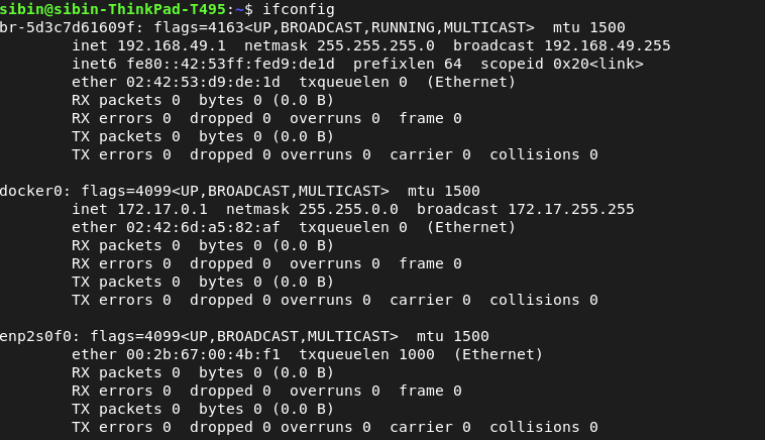
\includegraphics[width=1\textwidth]{SOA/NIC.png}
\end{figure}

\subsection{Maximum Transmission Unit}

The MTU decides the maximum packet size that can be transmitted over a network without being subject to fragmentation (splitting of packets). In the images above it is seen that all the network interfaces have an MTU of 1500 Bytes. In order to work with larger sized data, modiications to the protocols MTU must be done to accomadate the changes




\subsection{Packets}

Packets are bundled units of data that is transmitted across network interfaces. It is idenitified as: bits  for Physical Layer, frames for Data Link, packets for Network, and segments or datagrams for Transport Layer. For HTTP/3 App data, Ethernet frames encapsulates IP packets which contain UDP datagrams which carry QUIC Pakcets with multiple streams enabling multiplexing.

\begin{figure}[H]
\caption{Flow of Packets}
\centering
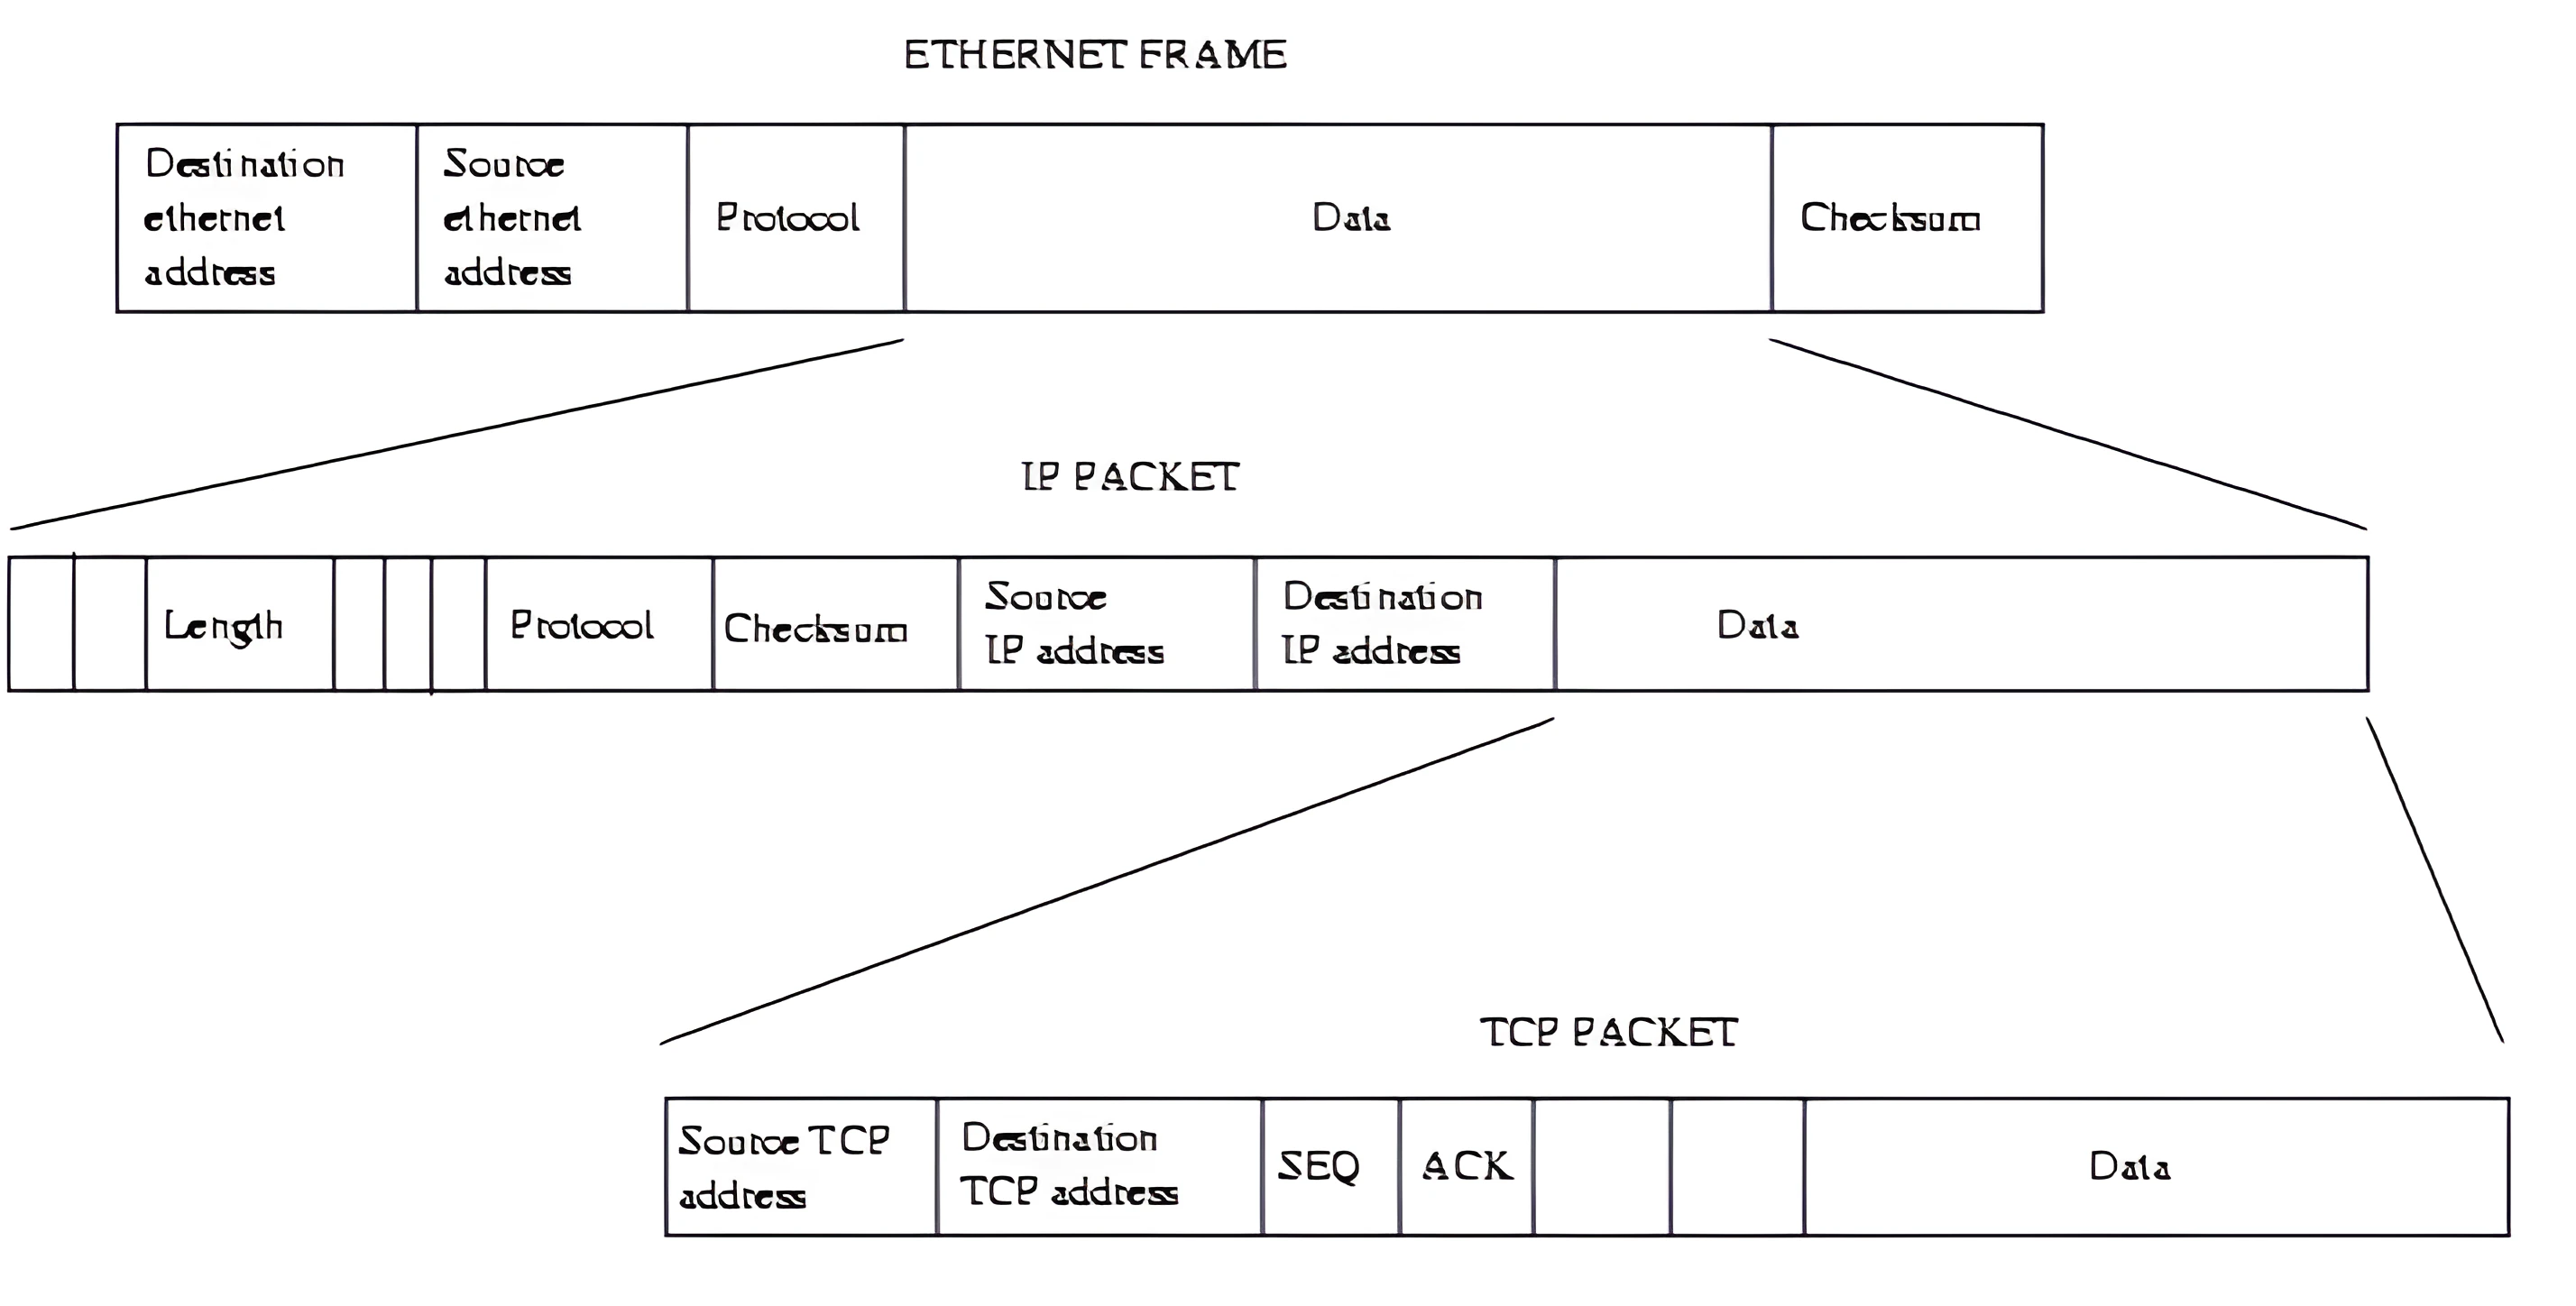
\includegraphics[width=1\textwidth]{SOA/packets.png}
\end{figure}

\subsection{Transmission Control Protocol}


Transmission Control Protocol (TCP) is a connection oriented protocol which ensures data reliability with several mechanisms such as Acknowledgments (Acks), Retransmissions and in-order delivery \cite{kurose2017}. TCP functions by establishing a three-way handshake between client and server. The handshakes can be seen in the figure below. TCP requires roundtrips to initiate communication and when it works with higher level application protocols which require TLS, it impacts performance introducing latency particularly during the connection setup.


\begin{figure}[H]
\caption{TCP Handshake}
\centering
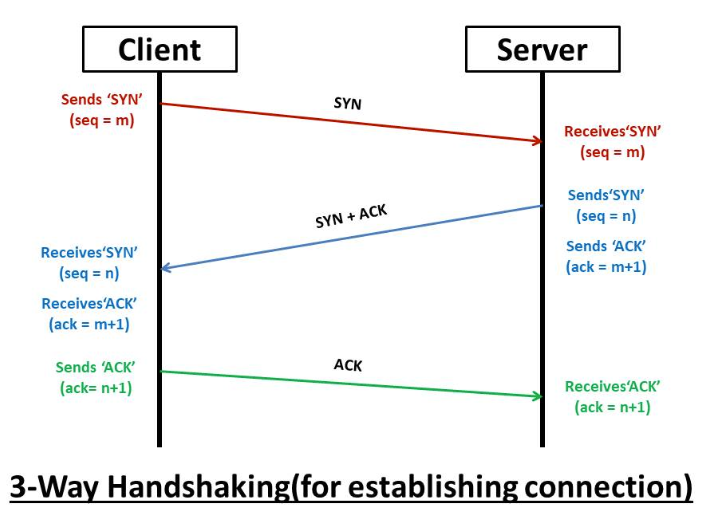
\includegraphics[width=0.7\textwidth]{SOA/tcp.png}
\end{figure}


TCP's design introduced challenges such as Head of Line Blocking. This is an issue which impacts performance for applications at scale. This HoL problem basically means that when a packet is lost, all subsequent packets are waited until the packet reaches the destination. Several approaches are followed to mitigate this issue such one such approach is multi-path TCP where data is sent over multiple paths avoiding this issue but the underlying protocol still suffers from this issue and the middlebox configuration is a concern.

TCP guarantees reliability making it ideal for application which require stringent ordered delivery. However, due to middle box configurations and TCPs reliance on outdated implementations restricts it from being highly performative.


\subsubsection{Operating System Configurations for TCP}

In linux machines, TCP's state is exposed  through the /proc/next/tcp path which is a virtual filesystem part of the procfs interface. This provides dynamically generated real time information about the active TCP connections which includes local addresses, remote addresses, port numbers, connection states and sequence number. Each entry persists for 60s  in the TIME\_WAIT state. (Protocol Compliance Requirement). The confgurations for handling concurrent tcp connections are monitored via parameters such as tcp\_max\_orphans, fs.file-max, and ulimit -n. Modification to these parameter increases the set limits to increase performance. 


\subsubsection{TCP Congestion and Flow Control}

TCP’s congestion control is managed by the sender with the congestion window ('cwnd'), its initialized with a small value at the start, such as 10 segments, and adjusted based on network feedback from the server. During the slow start phase, 'cwnd' grows exponentially with reception of acknowledgments (ACKs), when a packet loss is detected via duplicate ACKs or timeouts, it triggers a reduction in 'cwnd' to mitigate network congestion with the help of flow control which is managed by the receiver’s advertised window ('rwnd'), it prevents buffer overflow by limiting the sender’s transmission rate.





\subsection{Middle-Box Ossification}
Middleboxes become bottlenecks because of its old implementation and inability to update widely adopted middleboxes. In context of tcp it means the network devices like firewalls, routers have tcp implementation at their kernel level, which becomes an issue when updates to the core implementation of protocol are required.


\subsection{User Datagram Protocol}

User Datagram Protocol (UDP), is a connectionless protocol that focuses low latency than reliability \cite{kurose2017}. This is due to the fact that it lacks the built-in mechanisms for retransmission, ordering, or congestion control and hence makes it suitable for applications where speed is critical, and occasional packet loss is tolerated. Due to this it enables one-RTT communication which is ideal for Domain Name System (DNS) queries and real-time media streaming like online gaming, video streaming, etc. But, its lack of reliability, security, and congestion control makes it unsuitable for use in cases requiring guaranteed delivery.

\subsubsection{UDP Packet Structure}

UDP operates within a simple packet structure encapsulated as follows:

\begin{itemize}
    \item \textbf{Ethernet Frame}: It contains the Media Access Control (MAC) addresses(source and destination) and the control information for physical transmission.
    \item \textbf{IP Packet}: It encapsulates the source and destination IP addresses for routing.
    \item \textbf{UDP Datagram}: It includes the source and destination ports and the data(payload), with no reliability or ordering mechanisms.
\end{itemize}

UDP’s minimalist design enables low-latency communication but it lacks the robust features of TCP, and hence it requires application-level handling of reliability and ordering where needed.

UDP, lacking connection state, does not maintain persistent entries in /proc(the virtual filesystem used to expose kernel and process information). Both protocols face challenges with middleboxes(see section 2.1.7), such as firewalls, which often rely on outdated TCP configurations, complicating updates for advanced features like TCP Fast Open.

\subsection{Limitations of Traditional Transport Layer Protocols}

The foundational transport protocols of the internet, TCP and UDP, face well-documented limitations that hinder performance, scalability, and adaptability in modern network environments.

TCP suffers mostly from \textit{head-of-line (HOL) blocking}, a condition where the loss of a single packet holds up the delivery of all subsequent packets in that stream, thereby leading to increase in latency and degrading user experience. In addition to internal limitations, TCP evolution is impeded by \textit{middlebox ossification} see section 2.1.7. Network devices like legacy firewalls and Network Address Translation (NAT) gateways often do not recognize newer TCP features, such as, TCP Fast Open or Multipath TCP, blocking their deployment and stalling protocol innovation across the wider internet.

On the other hand, UDP, designed as a minimal transport layer, circumvents many of TCP’s internal restrictions but introduces its own set of challenges. It lacks built-in mechanisms for reliability, packet ordering, and congestion control, forcing developers to reimplement these features at the application level. Moreover, UDP is susceptible to \textit{NAT rebinding}, where NAT devices revoke and reassign port mappings after idle periods, leading to unexpected connection drops.

Both TCP and UDP also has  host-level limitations. Important among these is the finite ephemeral port range, typically around 65,000 ports per IP address which restricts the number of simultaneous connections to the same destination. In high-throughput systems, the availability of file descriptors and system memory further limits the scale of concurrent network connections, imposing additional resource constraints.

These protocol-level and systemic challenges have led to the development of next-generation transport protocols like QUIC, that aim to address these shortcomings in a modern, application-aware manner.

\subsection{QUIC Protocol}

The Quick UDP Internet Connections (QUIC) protocol represents an innovative transport layer solution designed to address the limitations of traditional TCP-based protocols, particularly in the context of modern web applications. Unlike TCP, which relies on sequential TLS and TCP handshakes, QUIC leverages UDP to combine transport and security handshakes into a single step, significantly reducing connection setup latency.

QUIC’s design aims to provide TCP-like reliability, stream multiplexing, and congestion control (see section 2.1.10.2) while mitigating TCP’s drawbacks, such as HOL blocking and the need for kernel-level updates across network infrastructure. By operating over UDP, QUIC enables deployment without requiring modifications to middleboxes like firewalls or routers, which often struggle with outdated TCP configurations. 

QUIC is a transport protocol that integrates the TLS 1.3 handshake with its initial transport handshake, achieving connection setup in a single RTT. QUIC also incorporates reliability, in-order delivery, and congestion control, addressing UDP’s limitations while retaining its low-latency characteristics. The protocol supports multiplexing through independent streams within a single connection, eliminating inter-stream HOL blocking, a significant issue in TCP-based HTTP/2. 

\subsubsection{QUIC Packet Structure}

QUIC operates within a layered architecture, encapsulated as follows:

\begin{itemize}
    \item \textbf{Ethernet Frame}: Contains MAC addresses and control information for physical transmission.
    \item \textbf{IP Packet}: Encapsulates source and destination IP addresses for network routing.
    \item \textbf{UDP Datagram}: Provides a lightweight, connectionless transport layer for QUIC packets.
    \item \textbf{QUIC Packet}: Includes a header, such as Short Header with Destination Connection ID and Packet Number, and an encrypted payload containing frames such as ACK, STREAM, and datagram frames.
\end{itemize}

\begin{figure}[H]
\caption{QUIC vs TCP packet Structure}
\centering
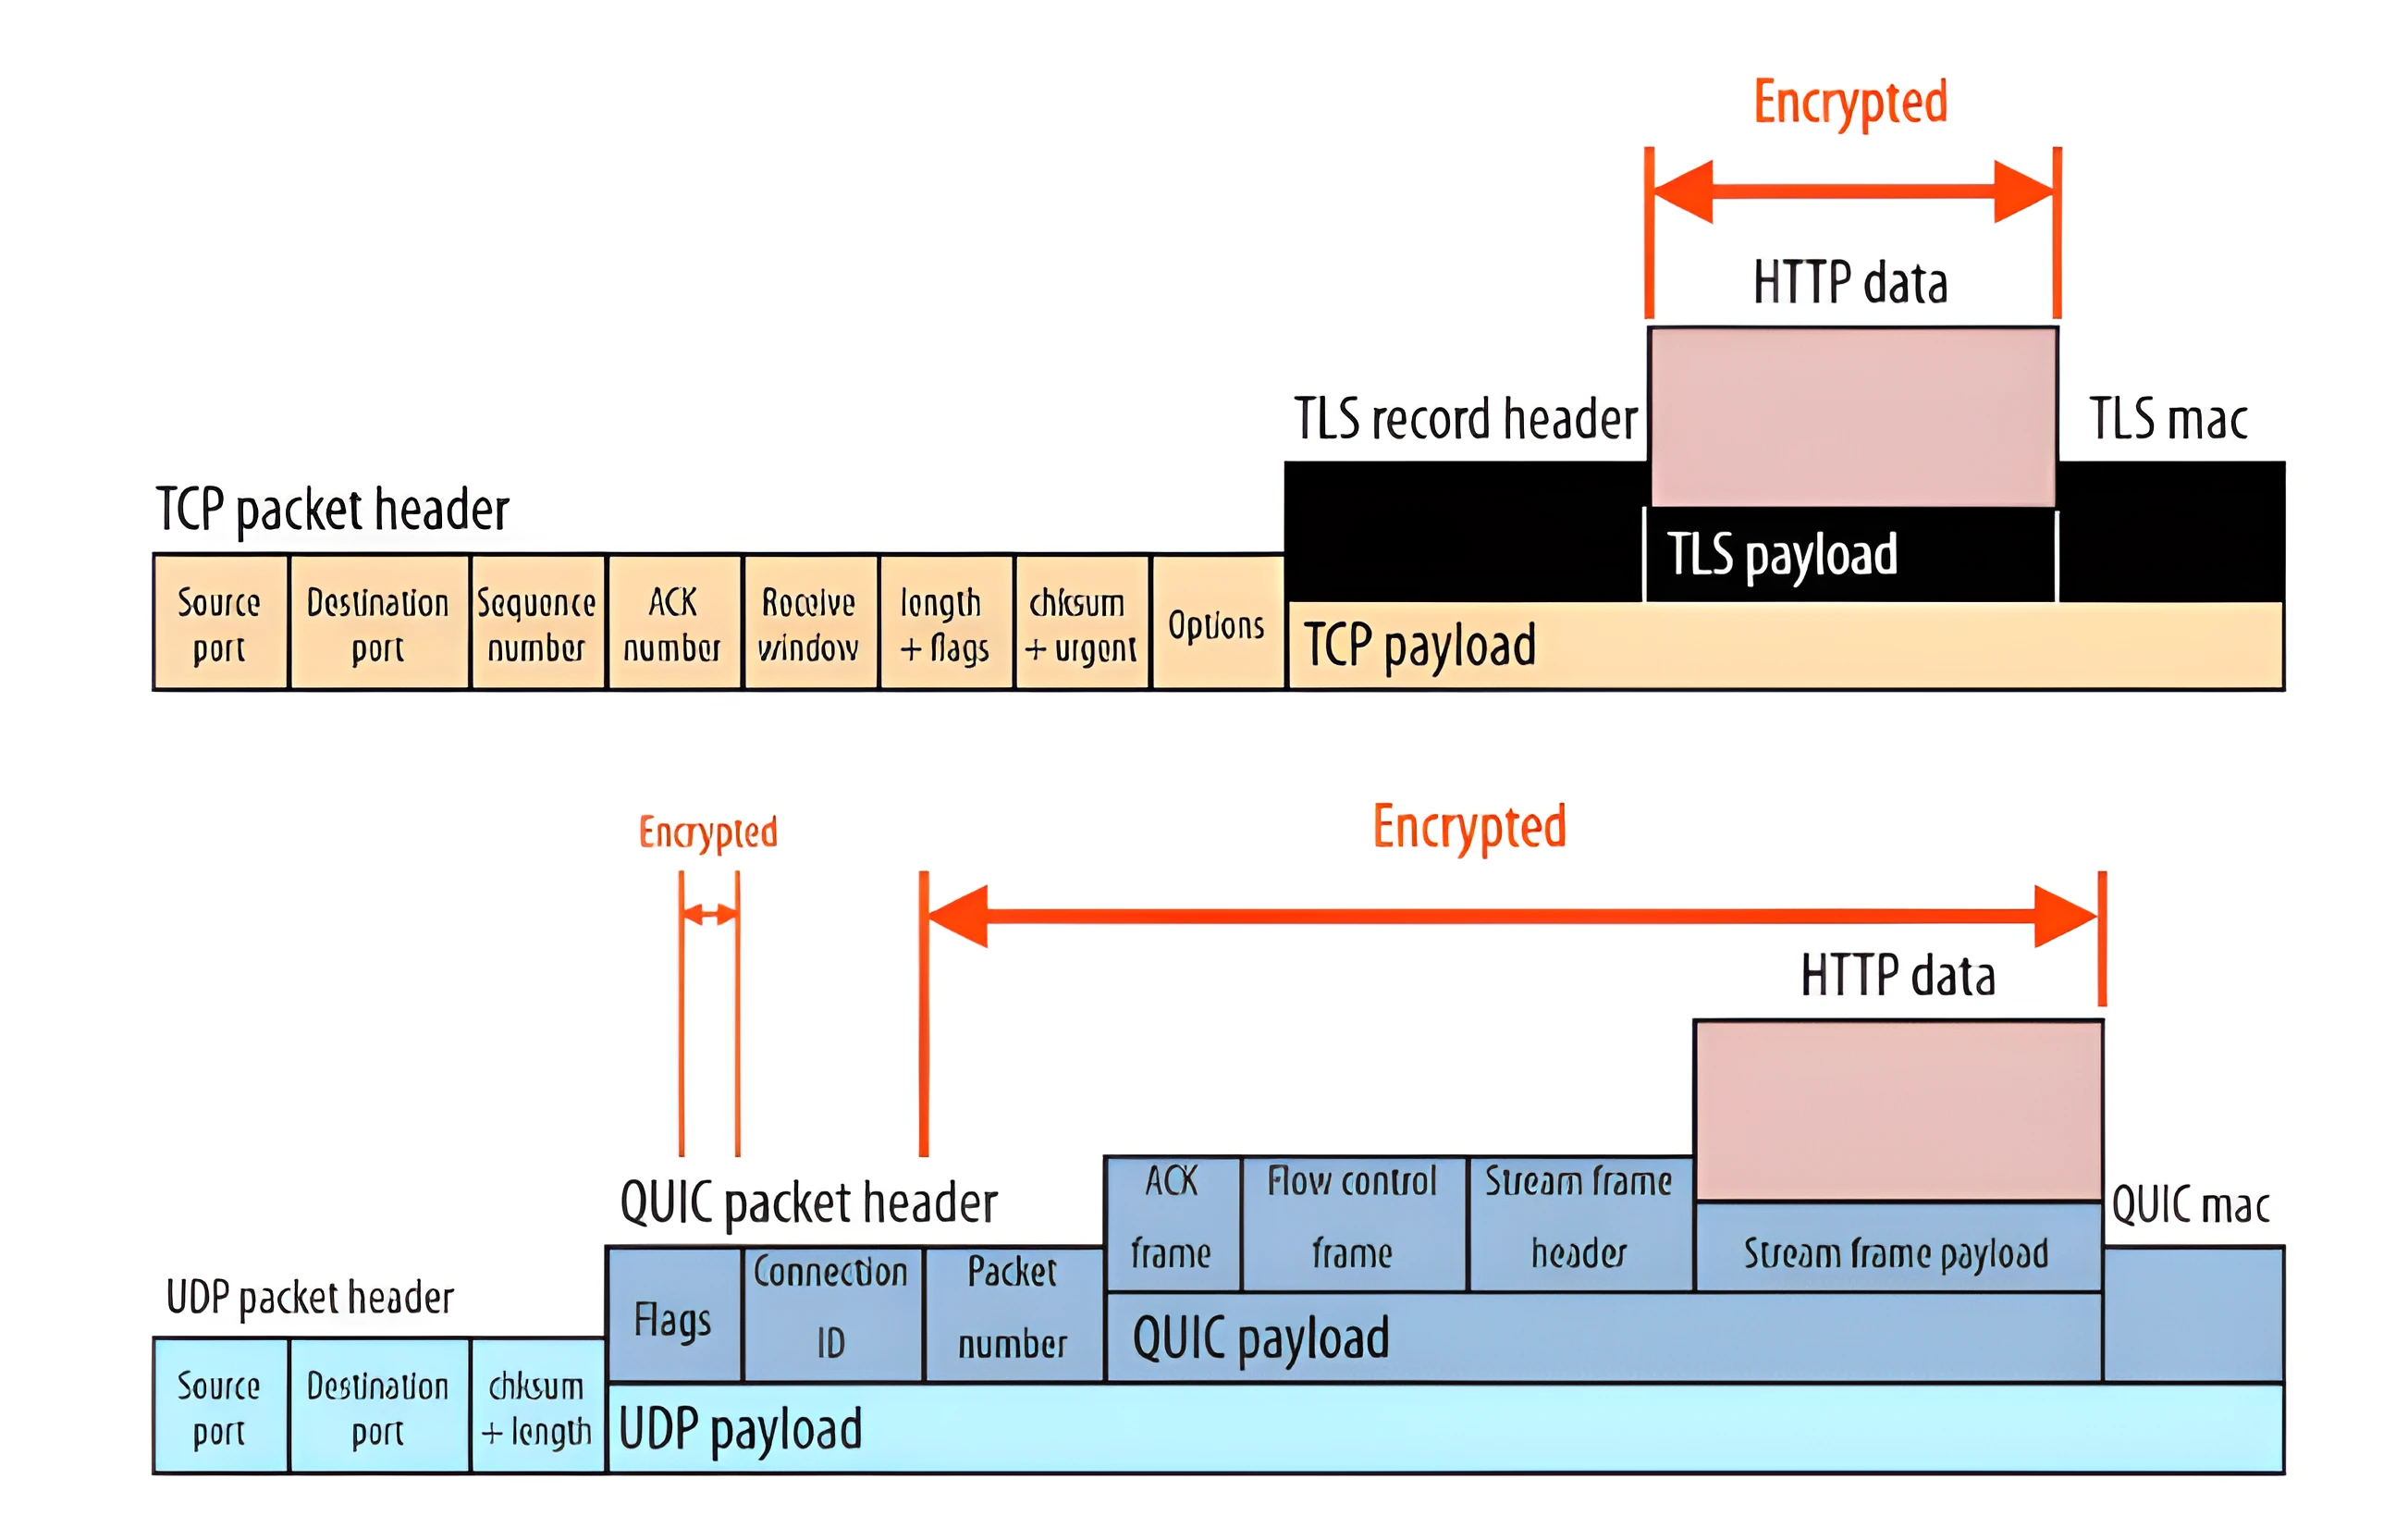
\includegraphics[width=1\textwidth]{SOA/quicntcp.png}
\end{figure}


For example, in above figure \cite{marx2021-http3} depicting QUIC Packet structure we can see that quic packets are sent as a udp packet in its payload


\subsubsection{Congestion and Flow Control}

QUIC implements congestion control at the connection level, using a sender-managed congestion window (\texttt{cwnd}) that adjusts based on network conditions, similar to TCP. The sender initializes \texttt{cwnd} conservatively, such as 10 segments, and increases it exponentially during the slow-start phase or linearly during congestion avoidance, reducing it upon detecting packet loss. Flow control, managed by the receiver’s advertised window (\texttt{rwnd}), operates at the stream level, ensuring that senders do not overwhelm receiver buffers.

Stream prioritization, supported by QUIC’s APIs, allows developers to assign higher priority to critical streams such as audio over video, optimizing resource allocation. Frame coalescing further enhances efficiency by packing multiple frame types into a single UDP datagram, following the Maximum Transmission Unit (MTU).

\subsubsection{Implementation Considerations}

QUIC’s user-space implementation, unlike TCP’s kernel-space design, enables rapid iteration but introduces performance overhead. Debugging tools like \texttt{qlog} and \texttt{qvis} facilitate debugging and analysis of QUIC’s advanced features, such as multiplexing and congestion control. For large file downloads, QUIC supports range-based requests which is similar to HTTP Range headers, allowing recovery of broken connections by requesting only missing byte ranges, provided servers support partial content requests.

QUIC’s ability to multiplex streams and datagrams within a single connection enhances its suitability for applications requiring concurrent data transfers, such as web browsing and file downloads. However, intra-stream HOL blocking persists, as data within a single stream is delivered in order, requiring retransmission of lost packets before subsequent data can be processed. In this dissertation implementation, we will be focusing on the feature multiplexing (multiple independent streams per connection).

\subsection{Comparison of TCP, UDP, and QUIC}

The following table summarizes the key features of QUIC compared to TCP and UDP, highlighting its hybrid design:

\begin{table}[H]
\centering
\begin{tabular}{|p{4cm}|c|c|c|}
\hline
\textbf{Feature} & \textbf{UDP} & \textbf{TCP} & \textbf{QUIC} \\
\hline
Connectionless & Yes & No & Yes (UDP-based) \\
\hline
Reliable Delivery & No & Yes & Yes \\
\hline
In-Order Delivery & No & Yes & Yes (per stream) \\
\hline
Multiplexing & No & No & Yes (multiple streams per connection) \\
\hline
Built-in TLS & No & No (external TLS) & Yes (TLS 1.3 mandatory) \\
\hline
Head-of-Line Blocking & No & Yes (affected) & No (avoids inter-stream blocking) \\
\hline
Connection Migration & No & No & Yes (survives IP changes) \\
\hline
\end{tabular}
\caption{Comparison of features across UDP, TCP, and QUIC}
\label{tab:tcp-udp-quic-comparison}
\end{table}



\section{HTTP Protocols}

The HyperText Transfer Protocol (HTTP) has undergone multiple changes since its inception, which helped it evolve in order to meet the growing demands of modern web applications. Each version introduces significant changes in how data is structured, delivered, and optimized over networks.
\begin{figure}
\centering
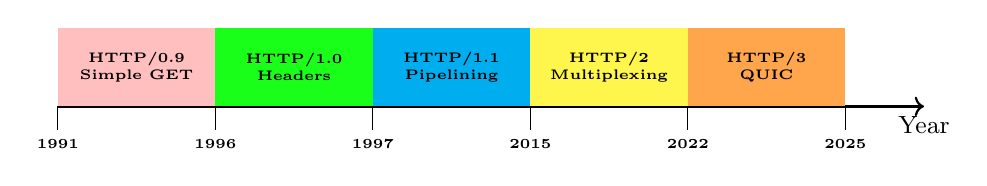
\begin{tikzpicture}[scale=1]
% Drawing the timeline axis
\draw[->, thick] (0,0) -- (11,0) node[below, font=\small] {Year};

% Year ticks and labels
\foreach \x/\year in {0/1991, 2/1996, 4/1997, 6/2015, 8/2022, 10/2025} {
  \draw (\x,0) -- ++(0,-3mm) node[below, font=\tiny\bfseries] {\year};
}

% HTTP version bars with simplified labels
\fill[pink] (0,0) rectangle ++(2,1) node[midway, black, font=\tiny\bfseries, align=center] {HTTP/0.9 \\ Simple GET};
\fill[green!90] (2,0) rectangle ++(2,1) node[midway, black, font=\tiny\bfseries, align=center] {HTTP/1.0 \\ Headers};
\fill[cyan] (4,0) rectangle ++(2,1) node[midway, black, font=\tiny\bfseries, align=center] {HTTP/1.1 \\ Pipelining};
\fill[yellow!70] (6,0) rectangle ++(2,1) node[midway, black, font=\tiny\bfseries, align=center] {HTTP/2 \\ Multiplexing};
\fill[orange!70] (8,0) rectangle ++(2,1) node[midway, black, font=\tiny\bfseries, align=center] {HTTP/3 \\ QUIC};

\end{tikzpicture}
\caption{HTTP protocol evolution (1991--2025)}
\label{fig:http-timeline}
\end{figure}


As shown in Figure~\ref{fig:http-timeline}, the HTTP protocol evolved significantly from 1991 to 2025, introducing key features like multiplexing and QUIC.

\subsection{HTTP/0.9}

Introduced in 1991, HTTP/0.9 was the earliest version of the protocol, designed for the simple retrieval of HTML documents. It supported only the \texttt{GET} method, and responses consisted of raw HTML without headers. Lacking support for metadata, status codes, or content types, HTTP/0.9 was limited to extremely basic use cases. It operated over a single TCP connection and closed the connection immediately after the response, making it inefficient for handling multiple resources.

\subsection{HTTP/1.0}

HTTP/1.0, standardized in 1996 (RFC 1945), introduced significant improvements over HTTP/0.9. It added support for additional HTTP methods such as \texttt{POST} and \texttt{HEAD}, HTTP headers for metadata exchange, status codes to indicate request outcomes, and support for different content types beyond HTML. HTTP/1.0 also introduced the concept of request and response headers, enabling features like content negotiation, caching directives, and authentication mechanisms.

However, HTTP/1.0 maintained the limitation of opening a new TCP connection for each request-response cycle, leading to significant overhead. Each resource on a web page required a separate connection, resulting in multiple TCP handshakes and increased latency. This approach proved inefficient as web pages became more complex, incorporating multiple images, stylesheets, and scripts, highlighting the need for connection reuse mechanisms.

\subsection{HTTP/1.1}

Standardized in 1997 (RFC 2068, later updated by RFC 2616 and RFC 7230 series), HTTP/1.1 addressed the major limitation of HTTP/1.0 by introducing persistent connections, allowing multiple requests and responses to be sent over a single TCP connection \cite{kurose2017}. It added methods like \texttt{PUT}, \texttt{DELETE}, and \texttt{OPTIONS} and support for chunked transfer encoding, enhanced caching mechanisms, and virtual hosting through the \texttt{Host} header.

Despite these improvements, HTTP/1.1 suffered from head-of-line blocking at the application layer, which severely limited performance, particularly for resource-heavy web pages. This limitation arose from the protocol being fundamentally constrained by the serialized nature of TCP streams, where requests had to be processed sequentially.

\subsection{HTTP/2}

HTTP/2 was published in 2015 (RFC 7540), in order to fix the performance limitations of HTTP/1.1 \cite{kurose2017}. It introduced binary framing, header compression (HPACK), and multiplexing, allowing multiple concurrent streams over a single TCP connection. These changes led to significant reduction in latency and improved page load times. As HTTP/2 still has underlying TCP, it remains susceptible to TCP-level head-of-line blocking. If a packet is lost, the entire TCP connection stalls until retransmission is complete, affecting all multiplexed streams.

\subsection{HTTP/3}

HTTP/3 is an application-layer protocol built on top of QUIC, developed to overcome the limitations of HTTP/2, particularly head-of-line (HOL) blocking caused by its reliance on TCP \cite{rfc9114} \cite{marx2021-http3}. By replacing TCP with QUIC (which runs over UDP), HTTP/3 introduces features such as built-in encryption (TLS 1.3), reduced handshake latency, connection migration, and robust stream multiplexing. These capabilities make HTTP/3 ideal for modern web environments, including mobile-first, real-time, and high-throughput applications.

\subsubsection{Multiplexing, Flow Control, and Congestion Handling}

HTTP/3 benefits directly from QUIC’s architecture, which provides independent, multiplexed streams within a single connection. This means that packet loss on one stream doesn’t block others, resolving the HOL blocking issue thats present in TCP. It allows more efficient and smoother data delivery, especially over unreliable or variable networks.

QUIC also implements stream-level flow control, ensuring that each stream can progress without interfering with others. Additionally, it features advanced congestion control algorithms, such as BBR or CUBIC, similar to TCP, but designed to react faster and recover more effectively in poor network conditions. These mechanisms enable HTTP/3 to maintain low latency and high performance across diverse network environments.

HTTP/3, through QUIC, provides several key enhancements including faster connection establishment via reduced round trips, encryption by default using TLS 1.3, stream multiplexing without HOL blocking, connection migration in case of IP changes, such as switching from Wi-Fi to mobile data, and 0-RTT support allowing faster repeat connections.


\subsubsection{Implementation and Adoption}

HTTP/3 is supported by major implementations such as Google’s quiche, Cloudflare’s quiche, Mozilla’s neqo, and Facebook’s mvfst, with integration into popular web servers like nginx, LiteSpeed, and Apache. Browser support is strong, with Chrome, Firefox, Safari, and Edge already implementing HTTP/3.

However, widespread adoption is still in progress. Challenges such as middlebox compatibility, UDP tuning limitations, and infrastructure readiness hinders deployment. Nonetheless, as HTTP/3 continues to demonstrate tangible performance and reliability improvements, especially in mobile and high-latency scenarios, its adoption is steadily accelerating.


\subsection{Summary Table: HTTP Protocol Evolution}

\begin{table}[H]
\centering
\resizebox{\textwidth}{!}{%
\begin{tabular}{|l|c|c|c|c|c|}
\hline
Feature & HTTP/0.9 & HTTP/1.0 & HTTP/1.1 & HTTP/2 & HTTP/3 \\
\hline
Transport Layer & TCP & TCP & TCP & TCP & QUIC (UDP-based) \\
Methods Supported & GET only & GET, POST, HEAD & All standard methods & All standard methods & All standard methods \\
Headers & No & Yes & Yes & Yes (compressed) & Yes (compressed) \\
Status Codes & No & Yes & Yes & Yes & Yes \\
Persistent Connections & No & No & Yes & Yes & Yes \\
Multiplexing & No & No & No (pipelining only) & Yes (over TCP) & Yes (parallel over QUIC) \\
Header Compression & No & No & No & Yes (HPACK) & Yes (QPACK) \\
HOL Blocking (Transport) & N/A & N/A & Yes & Yes & No \\
Encryption & No & No & Optional (via TLS) & Optional (via TLS) & Yes (via QUIC) \\
\hline
\end{tabular}%
}
\caption{Evolution of HTTP protocol features across versions}
\end{table}


\section{WebSocket Protocol}

As HTTP protocols evolved to address performance limitations, another approach emerged to handle real-time, bidirectional communication needs: WebSocket. While HTTP/3 focused on improving request-response patterns through QUIC, WebSocket took a different path by establishing persistent, full-duplex communication channels over TCP.

WebSocket is a communication protocol that provides full-duplex communication channels over a single TCP connection. Standardized in RFC 6455, it was designed specifically for real-time web applications that require persistent connections between clients and servers. Unlike the request-response model of HTTP, WebSocket enables continuous, low-latency communication by keeping the connection open, eliminating the overhead of establishing new connections for each data exchange.

The protocol operates through an initial HTTP handshake that upgrades the connection to the WebSocket protocol. Once established, data can be sent bidirectionally without the constraints of HTTP headers or request-response cycles. This persistent nature makes WebSocket particularly suitable for applications requiring real-time updates, such as chat applications, online gaming, collaborative editing, and live streaming platforms.


\begin{figure}[h]
\centering
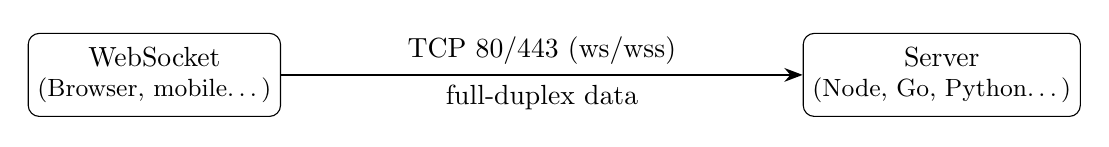
\begin{tikzpicture}[
    box/.style={rectangle, draw, rounded corners, minimum height=3em, minimum width=8em, align=center},
    arrow/.style={-Stealth, thick}
]
    % Nodes
    \node[box] (client)  at (0,0)   {WebSocket\\[-0.3ex]\small (Browser, mobile…)};
    \node[box] (server)  at (10,0) {Server\\[-0.3ex]\small (Node, Go, Python…)};
    
    % Arrows
    \draw[<->, arrow] (client.east) -- (server.west) 
          node[midway, above] {TCP 80/443 (ws/wss)} 
          node[midway, below] {full-duplex data};
\end{tikzpicture}
\caption{WebSocket Client-Server Connection}
\label{fig:websocket}
\end{figure}
Despite these advantages, WebSockets inherit limitations from their underlying transport layer, TCP. Because TCP enforces ordered, reliable delivery of data, packet loss on the network can cause head-of-line (HOL) blocking, where the delivery of later messages is delayed until missing packets are retransmitted. WebSockets also lack native multiplexing: all application data must share a single ordered stream, which can be suboptimal for applications needing parallel, independent data flows.

\section{WebTransport Protocol}

WebTransport is a modern protocol built over QUIC, designed to provide developers with flexible transport options for web applications. Unlike WebSockets, which rely on TCP and lack multiplexing, WebTransport leverages QUIC’s stream and datagram capabilities to support both reliable and unreliable data transfers within a single connection. WebTransport’s design enables developers to choose between streams for ordered, reliable delivery and datagrams for low-latency, loss-tolerant communication, making it suitable for diverse applications, including real-time gaming, audio streaming, and large file transfers.

WebTransport's architecture encapsulates data within QUIC packets, which are transmitted over UDP datagrams, IP packets, and Ethernet frames. This layered approach ensures compatibility with existing network infrastructure while providing advanced features like connection migration and frame coalescing. The protocol leverages QUIC's inherent capabilities to offer both reliable streams and unreliable datagrams within a single connection, allowing applications to use the most appropriate transport mechanism for different types of data - for instance, using streams for critical application state and datagrams for real-time position updates in gaming applications.

The protocol establishes a session over HTTP/3 using a CONNECT request, after which the connection is upgraded to support WebTransport-specific communication patterns. This design ensures compatibility with existing HTTP/3 infrastructure while enabling the advanced features that modern web applications require.

\subsection{WebTransport Streams}

WebTransport Streams provide a reliable, ordered, and flow-controlled mechanism for data transfer, analogous to TCP but with QUIC’s performance benefits. Each stream operates independently within a QUIC connection, identified by a unique Stream ID (Quic streams in background), allowing concurrent data transfers without inter-stream HOL blocking. For example, a single QUIC packet can carry multiple STREAM frames, such as HTML data and image data, as demonstrated in the provided content.

Streams are particularly suited for applications requiring guaranteed delivery, such as file downloads or structured data exchanges. However, intra-stream HOL blocking persists, as data within a single stream must be delivered in order, requiring retransmission of lost packets. Stream prioritization APIs enable developers to assign higher priority to critical streams - such as audio over video -, optimizing resource allocation. Due to their reliability and suitability for structured web applications, WebTransport Streams will be the focus of the implementation section of this dissertation.

\subsection{WebTransport API}

The WebTransport API is a modern JavaScript interface that enables web applications to communicate over QUIC, offering both reliable and unreliable transport options \cite{webtransport-mdn}. It is designed to support low-latency, multiplexed, and secure communication directly from the browser, making it ideal for use cases such as real-time gaming, video streaming, and collaborative applications.


\begin{figure}[H]
\centering
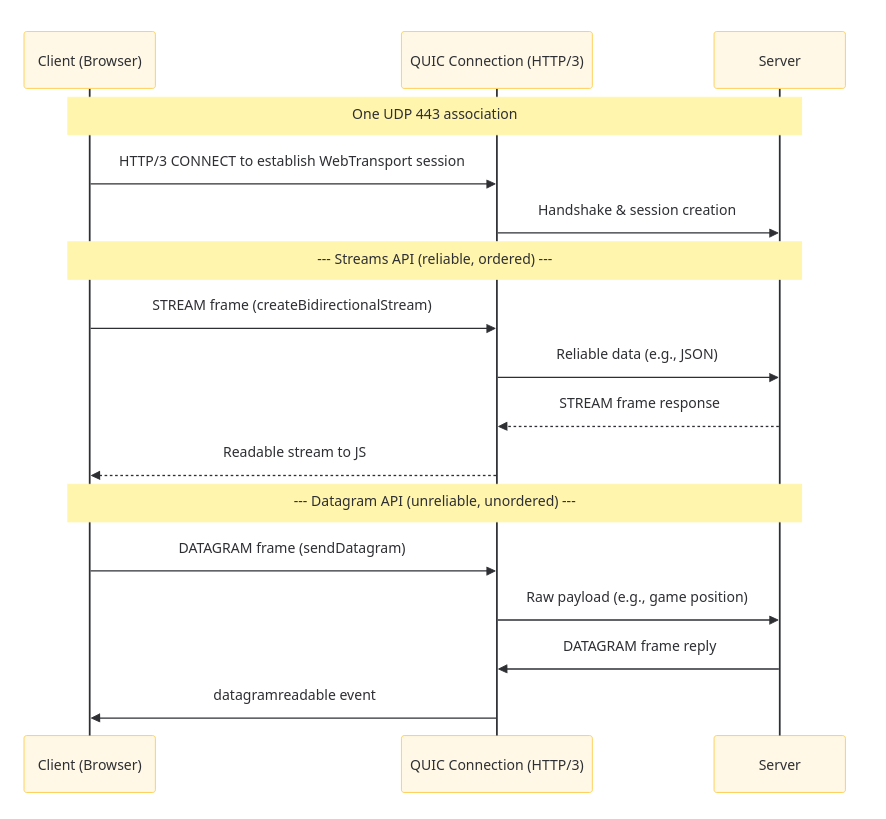
\includegraphics[width=0.8\textwidth]{SOA/webtransport_architecture.png}
\caption{WebTransport Architecture}
\label{fig:webtransport_architecture}
\end{figure}

Figure~\ref{fig:webtransport_architecture} illustrates a WebTransport session over HTTP/3, where a single UDP/443 connection is established between the client and server. After the HTTP/3 CONNECT request initiates the session through a QUIC handshake, the Streams API is used to create a reliable, ordered bidirectional stream for exchanging structured data such as JSON. In parallel, the Datagram API provides an unreliable, unordered channel for transmitting raw payloads, such as game state updates. Both communication types share the same QUIC connection and UDP socket, enabling efficient multiplexing of reliable and unreliable data within a single transport session.

WebTransport exposes two main interfaces for developers: the Streams API for reliable communication and the Datagram API for unreliable, low-latency communication. Understanding the practical implementation of these interfaces is crucial for building effective real-time applications.

\subsection{JavaScript Implementation}

The WebTransport JavaScript API provides developers with two primary interfaces for communicating over QUIC connections: the Streams API for reliable, ordered communication and the Datagram API for unreliable, low-latency communication. Understanding these implementation details is crucial for building real-time applications that leverage WebTransport's capabilities. This subsection examines the practical JavaScript syntax and usage patterns for both communication modes, providing concrete examples of how to establish connections, send data, and handle responses in web applications.

\subsubsection{Streams API – Reliable and Ordered Communication}

The Streams API provides bidirectional and unidirectional streams that ensure reliable, ordered data transfer. This makes it suitable for applications requiring robust delivery, such as sending structured HTML or JSON between a client and server.

Bidirectional Stream Example  
A client can open a stream and write data reliably to the server:

\begin{verbatim}
const transport = new WebTransport('https://example.com:4999'); 
await transport.ready; 

const stream = await transport.createBidirectionalStream(); 
const writer = stream.writable.getWriter(); 

await writer.write(new TextEncoder().encode('<html><head>')); 
\end{verbatim}

Unidirectional Stream Example  
Used for sending data in one direction only:

\begin{verbatim}
const stream = await transport.createUnidirectionalStream();
\end{verbatim}

These stream methods are part of the WebTransport session object. createBidirectionalStream() and createUnidirectionalStream() return stream instances, which can be accessed using .writable or .readable interfaces for sending and receiving data. Encoders like TextEncoder() convert strings into binary format suitable for transport.

\subsubsection{Datagram API – Unreliable and Unordered Communication}

The Datagram API allows for lightweight, unreliable, and unordered data exchange—perfect for scenarios where speed is prioritized over reliability, such as real-time positional updates in games or telemetry data.

Datagram Example:

\begin{verbatim}
const transport = new WebTransport('https://example.com:4999');
await transport.ready;

await transport.sendDatagram(new TextEncoder().encode('x:10,y:20'));
\end{verbatim}

The sendDatagram() function transmits a raw byte payload over QUIC datagrams. Since datagrams are not guaranteed to arrive or preserve order, developers must handle any necessary retries or loss-tolerance logic in the application layer.

\subsection{Custom Header Handling and Routing}

A key implementation challenge with WebTransport streams is the absence of built-in header support for content identification and routing. Unlike HTTP-based protocols that include headers to specify content type, routing information, and metadata, WebTransport streams require developers to embed this information within the data payload itself.

For example, when sending audio or video data over a stream, a header might be prefixed to indicate the type:

\begin{verbatim}
const header = 'audio';
const payload = new Uint8Array([...new TextEncoder().encode(header), ...binaryAudioData]);

await writer.write(payload);
\end{verbatim}

On the receiving end, such as in a server or reverse proxy, the application parses this prefixed header to determine how to route or process the incoming stream—such as directing it to the appropriate microservice, such as audio handler vs. video handler. While this provides flexibility, it introduces additional complexity in parsing logic and requires robust message framing techniques. This challenge will be explored further in the implementation section of this dissertation.

\subsection{Standardization Status and Future Outlook}

WebTransport represents an emerging approach to internet communication using modern web technologies. The protocol is currently defined in RFC 9297 for its HTTP/3 variant, though it has not yet achieved full standardization status. Similarly, the WebTransport API used in web browsers remains a Working Draft by the W3C, indicating that the specification may undergo changes before final standardization.

This evolving status presents both opportunities and challenges. While the protocol offers significant advantages over existing transport mechanisms, its ongoing development means that implementations may need to adapt to specification changes. This dynamic environment makes WebTransport an active area of research and innovation, particularly relevant for applications requiring low-latency, multiplexed communication.


\section{Wireshark}

Wireshark is a widely used open-source network protocol analyzer that allows real-time capture and inspection of network traffic across various protocols and interfaces. By selecting a network interface, such as Ethernet, Wi-Fi, or loopback, users can monitor all incoming and outgoing packets exchanged between a client and server. This level of visibility makes it an essential tool for network diagnostics, debugging, and protocol analysis, especially in complex distributed environments. Wireshark provides a graphical interface that breaks down packet details across different OSI layers, offering timestamps, protocol headers, payloads, and flow sequences.

One of Wireshark’s key features is its ability to decrypt encrypted traffic, including packets protected by TLS, provided the necessary session keys, such as pre-master secrets, are available. This is particularly useful when analyzing secure protocols like HTTPS, HTTP/3, or QUIC, which rely heavily on TLS 1.3 for encryption. By decrypting the payload, Wireshark enables developers and analysts to troubleshoot issues related to application-layer behavior, latency, or data integrity, even within secure connections (See  section 5.4.3 in implementation). This powerful functionality makes Wireshark a critical tool for both performance tuning and ensuring secure, reliable communication across networks. We will leverage this tool for our implementation in order to understand what exactly is going on.


\begin{figure}[H]
\centering
\begin{minipage}{0.9\textwidth}
  \centering
  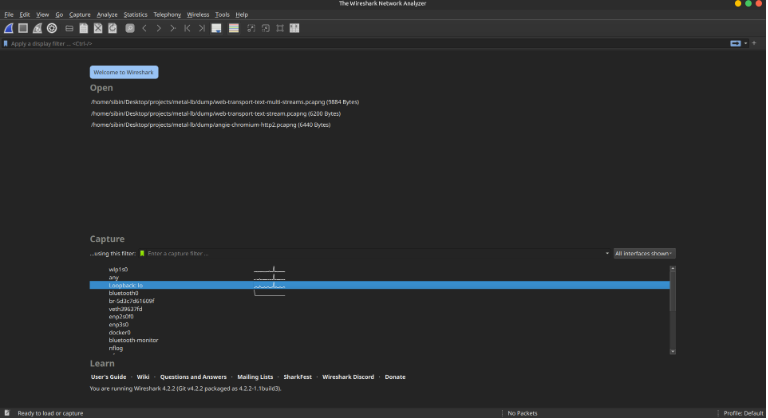
\includegraphics[width=\textwidth]{SOA/ws_interfaces.png}
  \caption{Network Interfaces}
  \label{fig:ws_interfaces} % optional label for referencing
\end{minipage}
\hfill
\begin{minipage}{0.9\textwidth}
  \centering
  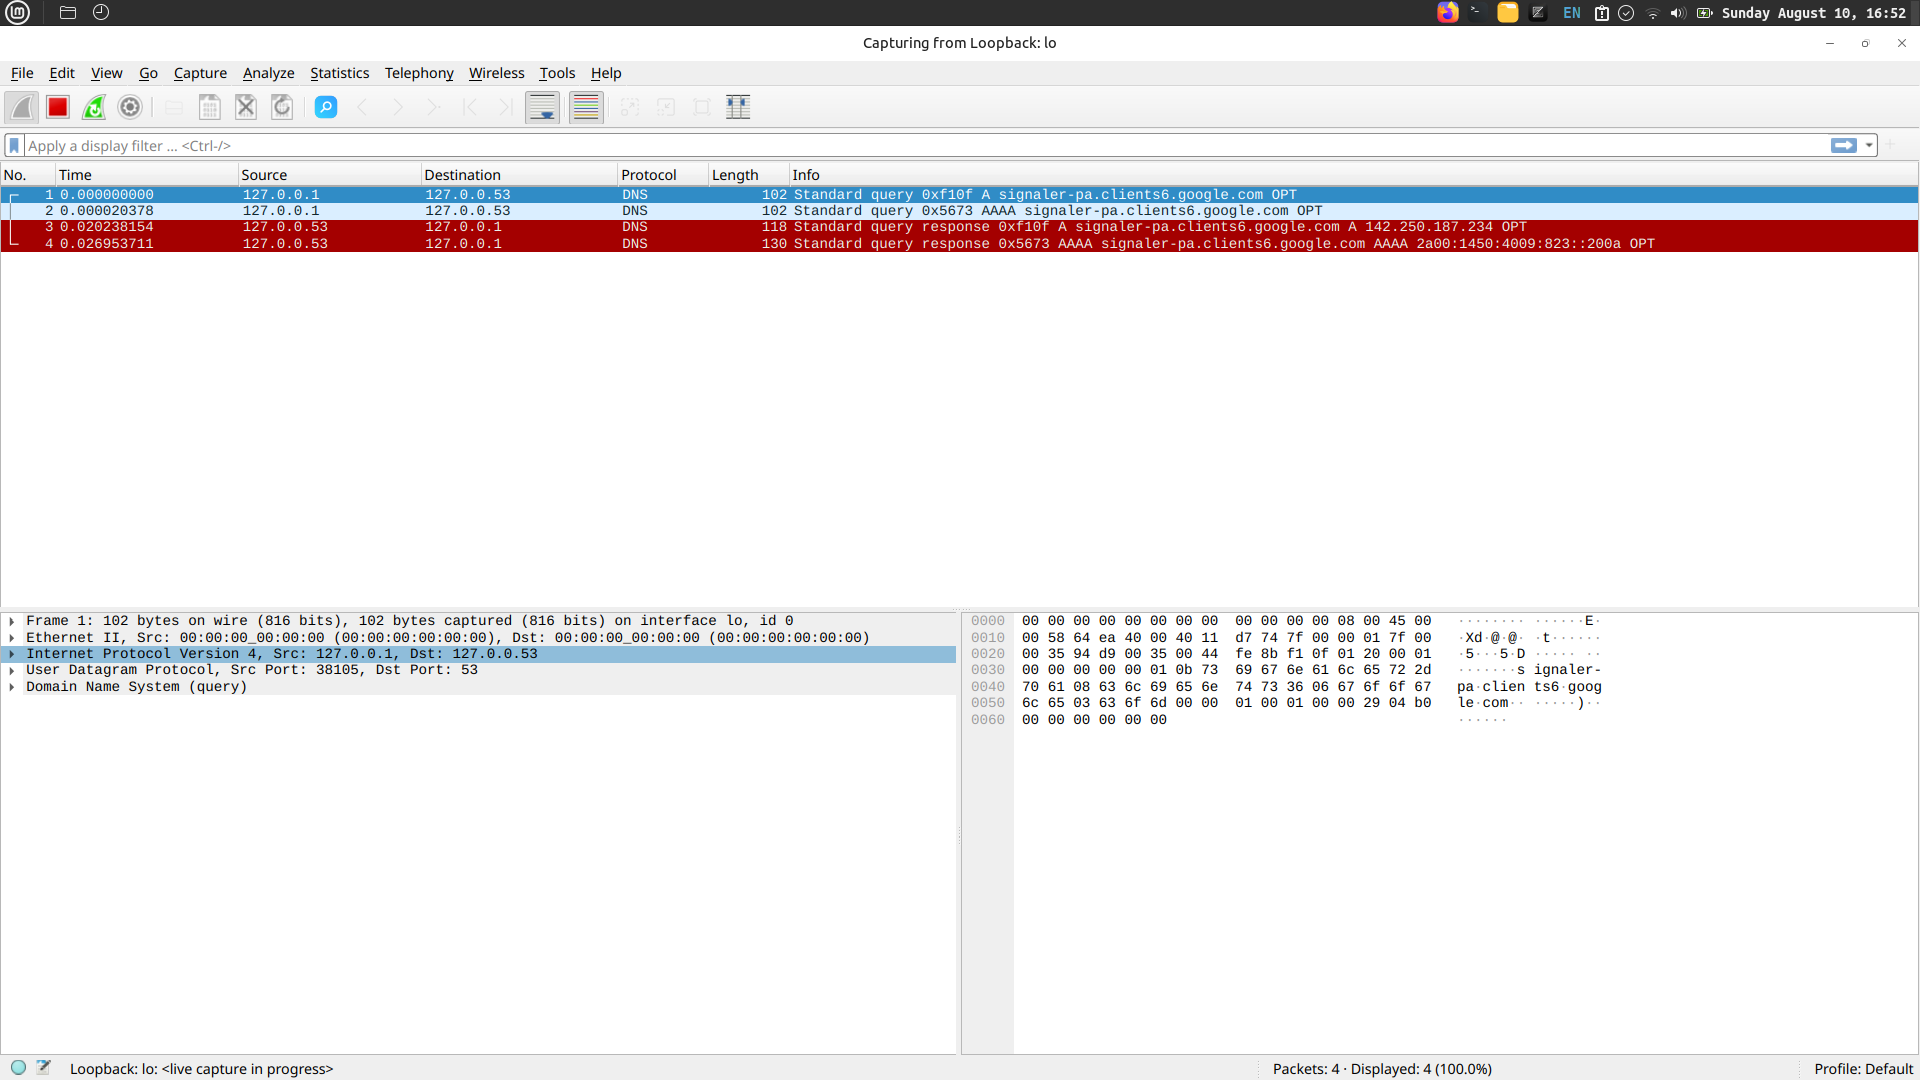
\includegraphics[width=\textwidth]{SOA/ws_packets.png}
  \caption{Network Packets}
  \label{fig:ws_packets} % optional label for referencing
\end{minipage}
\end{figure}

Figure~\ref{fig:ws_interfaces} and Figure~\ref{fig:ws_packets} above illustrates the Wireshark interface, showing the available network interfaces and captured packets. The left side displays the list of interfaces, while the right side shows the captured packets in the loopback interface with detailed information about each packet's protocol, source, destination, and other relevant metadata.

\section{Containers}
Containers are lightweight, portable, and consistent runtime environments that package an application along with all its dependencies, configuration files, and system libraries. Unlike traditional virtual machines, containers share the host operating system kernel, making them faster to start and more resource-efficient. Containers are created with a container image and all the information is bundled into an image and stored in a registry. This makes it ideal for deploying and scaling applications in a microservices architecture. In context for this dissertation, in order to deploy and run applications in Kubernetes, the prerequisite is having a Docker image ready.

\section{Kubernetes Concepts}

Kubernetes has emerged as the de facto standard for container orchestration, providing the infrastructure needed to deploy, scale, and manage containerized applications in production environments. For this dissertation's focus on WebTransport and QUIC-based streaming applications, understanding Kubernetes is essential as it provides the platform for deploying and managing the distributed microservices architecture. This section explores Kubernetes architecture, its core components, networking models, and the challenges and solutions for supporting modern protocols like HTTP/3 and WebTransport in containerized environments.

\subsection{Kubernetes Architecture Overview}
Kubernetes is built on a distributed architecture consisting of a Control Plane and multiple Worker Nodes. The Control Plane manages the cluster's desired state and handles decisions such as scheduling, scaling, and responding to cluster events. It includes components like the API Server, etcd - a consistent, distributed key-value store -, Scheduler, and Controller Manager. The Control Plane acts as the brain of the system, making high-level decisions and continuously monitoring and adjusting the cluster to match the user-defined configuration.

The Worker Nodes run the actual containerized applications. Each node hosts essential services: the kubelet (which ensures containers are running properly as specified by the control plane), the container runtime, such as containerd, and the kube-proxy, which handles networking and service discovery. Kubernetes follows a declarative model, where users define the desired state, such as the number of replicas, image versions, etc., and the system uses control loops to match the actual state with the desired state, ensuring continuous compliance and fault tolerance. Various core components within these layers work together to ensure reliability, scalability, and self-healing of applications across the cluster.

\subsection{Kubernetes Components}

Kubernetes operates through a collection of interconnected components that work together to manage containerized applications across a cluster. These components are divided between the control plane, which manages the overall cluster state and makes decisions, and the worker nodes, which run the actual application workloads. Understanding these components is crucial for comprehending how Kubernetes schedules, manages, and maintains applications, especially when deploying modern protocols like HTTP/3 and QUIC-based services. This subsection examines each core component and its role in the Kubernetes ecosystem.

\begin{figure}[H]
\centering
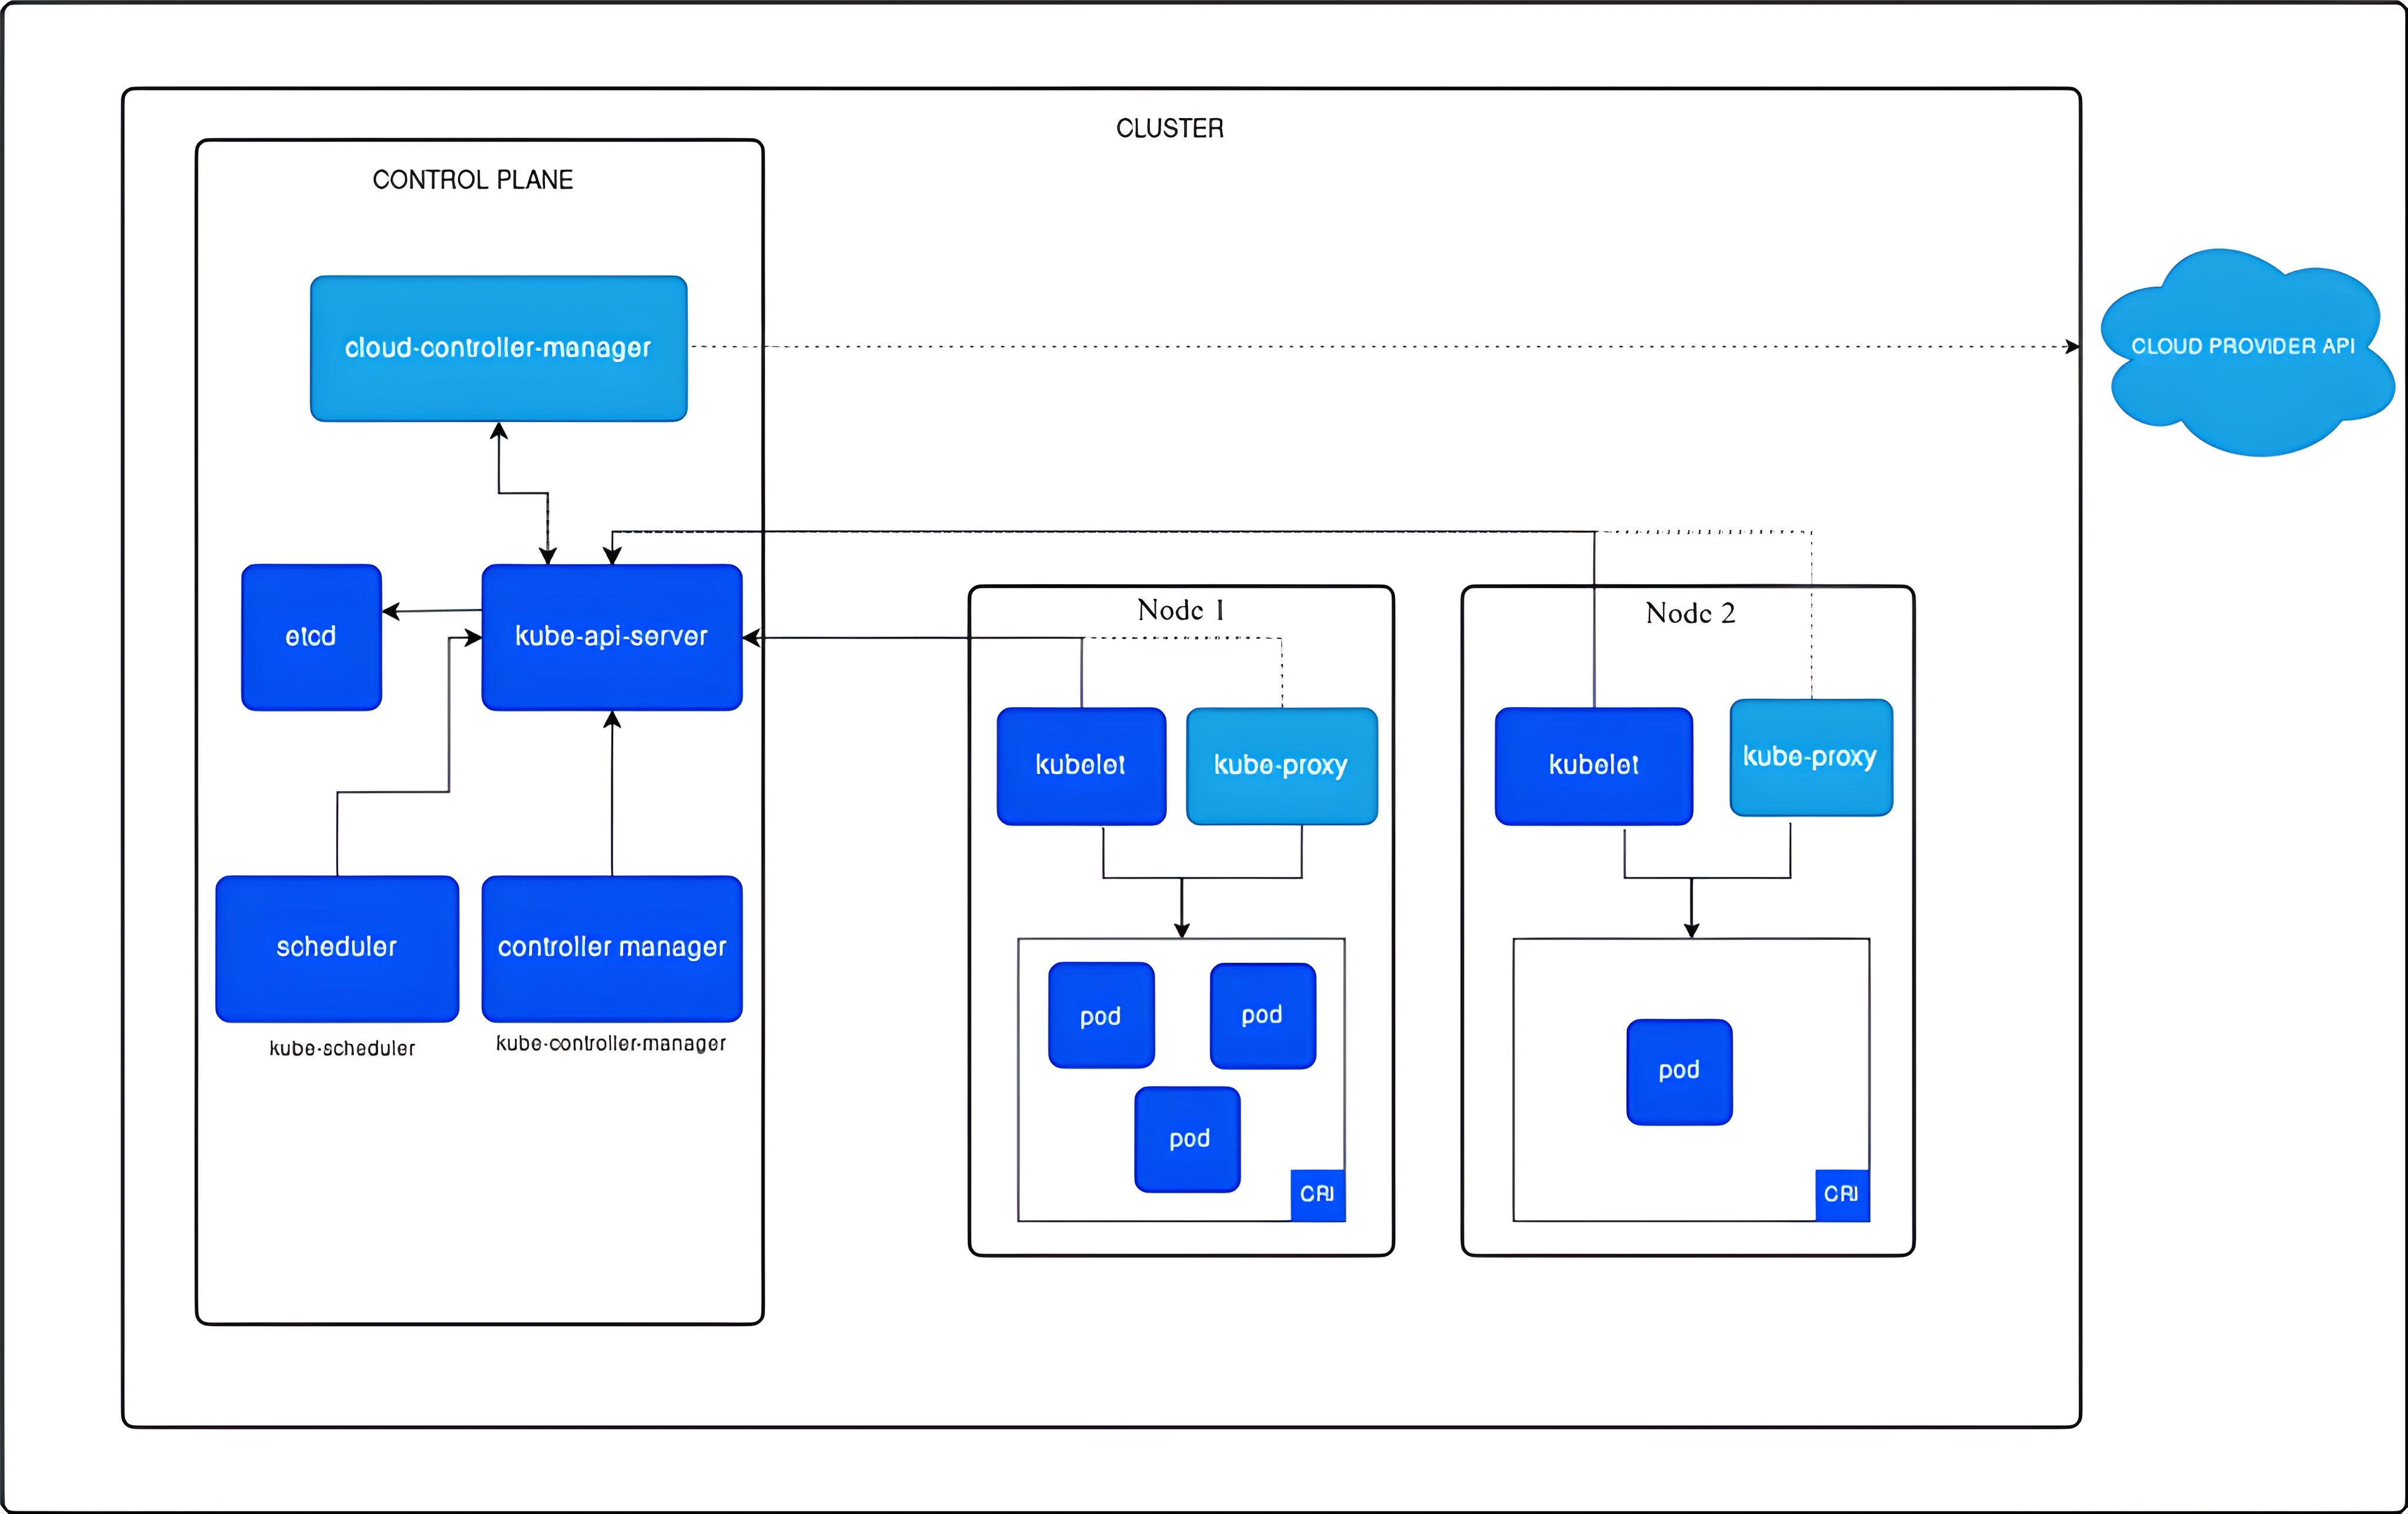
\includegraphics[width=1\textwidth]{SOA/kubernetes-cluster-architecture.png}
\caption{Kubernetes Architecture and Components}
\label{fig:k8s-architecture}
\end{figure}

Figure~\ref{fig:k8s-architecture} illustrates the complete Kubernetes architecture, showing the separation between the control plane components such as API Server, etcd, Scheduler, Controller Manager and the worker node components such as kubelet, kube-proxy, container runtime. This architecture follows the official Kubernetes design principles as documented in the Kubernetes documentation \cite{kubernetes-docs}.

\subsubsection{API Server}
The Kubernetes API Server (kube-apiserver) serves as the central management interface, exposing the Kubernetes API for communication between cluster components and external clients. It processes RESTful requests, validates and stores object configurations, such as Pods, Services, in the etcd database, and coordinates cluster operation. Any operation in the cluster goes through the API Server.

\subsubsection{etcd}
etcd is a distributed key-value store that maintains the cluster's configuration and state data, ensuring consistency and fault tolerance. It stores all Kubernetes objects, such as Pod definitions and Service configurations, providing a single source of truth for the control plane. The etcd allows to rollback to a previous cluster state.

\subsubsection{Controller Manager}
The Controller Manager (kube-controller-manager) runs control loops that monitor the cluster's state and match it with the desired state defined in manifests. It includes controllers like the Node Controller (managing node lifecycle), ReplicaSet Controller (ensuring pod replicas), and Service Controller (integrating with load balancers). 

\subsubsection{Scheduler}
The Scheduler (kube-scheduler) assigns pods to nodes based on resource requirements, constraints, and policies, such as affinity, taints. It optimizes resource utilization by evaluating node capacity and workload demands. For streaming use cases, the Scheduler ensures that Pulsar brokers or services are placed on nodes with sufficient resources, enhancing performance.

\subsubsection{Kubelet}
The Kubelet, running on each worker node, manages pod lifecycle by communicating with the API Server and container runtime, such as containerd, CRI-O. It ensures containers are running, healthy, and configured per pod specifications. In HTTP/3 deployments, Kubelets manage containers hosting QUIC-based services, as seen in prior Angie configurations.

\subsubsection{Kube-Proxy}
Kube-Proxy, also running on worker nodes, manages network rules to enable communication between pods, services, and external clients. It supports modes like iptables and IPVS, facilitating load balancing for services. In this dissertation, MetalLB setup \cite{metallb-docs}, Kube-Proxy worked alongside MetalLB to expose HTTP/3 services via UDP passthrough.

\subsubsection{Container Runtime}
The container runtime, such as containerd, CRI-O, executes containers within pods, handling image pulling, container creation, and lifecycle management. It interfaces with the Kubelet to ensure containers adhere to pod specifications.

\subsubsection{Storage Provisioner}
The Storage Provisioner dynamically allocates persistent storage to pods via PersistentVolumeClaims (PVCs) and PersistentVolumes (PVs) (see section 2.6.2.16). It interfaces with storage backends (ie volumes) to provision volumes based on StorageClass definitions. In this dissertation, for Apache Pulsar \cite{pulsar-helm-repo}, the Storage Provisioner ensures bookies have access to persistent storage for ledgers, supporting fault-tolerant data retention. Also configurations, involving MetalLB and Pulsar, relied on Storage Provisioners to manage storage for stateful workloads.

\subsubsection{CoreDNS}
CoreDNS, the default DNS service in Kubernetes, provides service discovery and name resolution within the cluster. Running as a pod, it resolves service names, such as http3-service.default.svc.cluster.local, to Pod IP addresses, enabling communication between pods and services. In HTTP/3 deployments, CoreDNS resolves backend service names for QUIC-based traffic, as seen in prior Angie and MetalLB setups. Its plugin-based architecture supports customization, such as integrating with external DNS providers.

\subsubsection{Namespaces}
Namespaces are logical separation of resources into groups. For example, all of the core architecture components run in a separate namespace kube-system.

\subsubsection{Pods}
A Pod is the smallest and simplest unit in the Kubernetes object model. It represents a single instance of a running process in a cluster. A pod can contain one or more containers that share the same network namespace, IP address, and storage volumes. Containers in the same pod can communicate using localhost and share mounted storage, making them ideal for tightly coupled workloads, such as a main app container and a sidecar for logging. Pods are ephemeral—once deleted or crashed, they aren't recreated unless managed by a higher-level controller like a Deployment or StatefulSet.


\begin{figure}[H]
\caption{Pods}
\centering
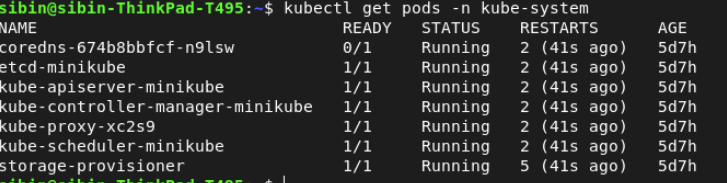
\includegraphics[width=1\textwidth]{SOA/k8s-components.png}
\end{figure}

The above figure shows the pods present in the namespace kube-system

\subsubsection{Deployments}
A Deployment is a controller that manages the lifecycle of pods. It ensures the desired number of pod replicas are running and updates them in a controlled manner. With deployments, users can perform rolling updates, rollbacks, and maintain zero downtime during application changes. When you update a deployment, such as to use a new container image, Kubernetes gradually replaces the old pods with new ones, ensuring stability throughout the process. Deployments abstract the complexity of pod creation and replication, offering scalability and resilience.

\begin{figure}[H]
\caption{Deployments}
\centering
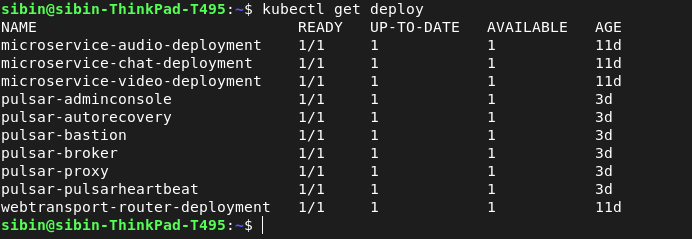
\includegraphics[width=1\textwidth]{SOA/k_deploy.png}
\end{figure}
The above figure illustrates the different deployment in the cluster's default namespace

\subsubsection{Services}
Kubernetes Services provide a stable networking endpoint to access pods, abstracting away their transient nature. Since pods have dynamic IPs and may be replaced, services ensure that applications or users can access workloads reliably. There are several types of services:

\begin{itemize}
    \item ClusterIP (default): Exposes the service on a cluster-internal IP. It is only accessible within the cluster, useful for internal communication between services.
    \item NodePort: Exposes the service on a static port (between 30000–32767) on each worker node's IP. Traffic to this port is forwarded to the underlying pods. It makes services accessible outside the cluster using  NodeIP:NodePort.
    \item LoadBalancer: Provisions an external load balancer (in cloud environments like Amazon Web Services (AWS) or Google Cloud Platform (GCP)) and routes traffic from the external world to the service. It provides a single external IP and balances traffic to the appropriate pods.
\end{itemize}

\begin{figure}[H]
\caption{Service}
\centering
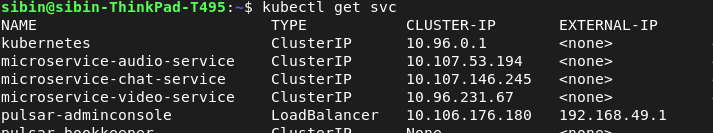
\includegraphics[width=1\textwidth]{SOA/k_svc.png}
\end{figure}
The above figure shows the services present in our cluster in default namespace.


If we are working with an internal service, go for default ClusterIP, and if you want to expose the service to the outside world, use NodePort or LoadBalancer.

\subsubsection{ConfigMaps}
ConfigMaps allows to externalize configuration from container images, separating application code from configuration data. They store key-value pairs that can be used to inject environment variables, command-line arguments, or configuration files into pods. This decoupling allows the same container image to be reused in different environments by simply changing the ConfigMap. For example, you could store database URLs, feature flags, or app settings without baking them into the container. In implementation microservice container image was deployed with config map.

\subsubsection{Secrets}
Secrets are similar to ConfigMaps but designed specifically for sensitive data like passwords, tokens, SSH keys, or certificates. Secrets are base64-encoded (not encrypted by default) and can be mounted as volumes or exposed as environment variables. They help protect confidential data by controlling access through RBAC and reducing the risk of hardcoding secrets into application images or code.

\subsubsection{Persistent Volumes (PVs) and Persistent Volume Claims (PVCs)}
Kubernetes provides an abstraction layer for storage through Persistent Volumes (PVs) and Persistent Volume Claims (PVCs). A PV is a piece of storage, such as a disk in a cloud provider or an NFS mount, provisioned by an admin or dynamically via StorageClasses. A PVC is a user's request for storage with specific requirements, such as size, access mode.

This decouples storage provisioning from storage consumption, allowing pods to request storage without knowing the details of the underlying storage infrastructure. PVs can outlive pods and enable stateful applications like databases to persist data even when pods are recreated.

\subsubsection{StatefulSets}
StatefulSets are a Kubernetes controller used to manage stateful applications that require stable network identities and persistent storage. Unlike Deployments, which treat all pods as interchangeable, StatefulSets assign each pod a unique, stable identity (including name and network address) and ensure ordered, graceful deployment, scaling, and deletion.

StatefulSets are ideal for workloads like databases, such as MongoDB, PostgreSQL, distributed systems, such as Kafka, ZooKeeper \cite{zookeeper-docs}, and any application that requires persistent storage tied to a specific pod. Each pod in a StatefulSet can be connected via a predictable DNS name and retains its associated PVC even when restarted.

\subsection{Cloud Kubernetes Clusters}
As Kubernetes adoption continues to rise across industries, cloud providers have responded with fully managed solutions to simplify deployment, scaling, and maintenance. Among the most prominent managed Kubernetes offerings are Amazon Elastic Kubernetes Service (EKS), Azure Kubernetes Service (AKS), and Google Kubernetes Engine (GKE). This section reviews these platforms, examining their design principles, cloud integration capabilities, and recent developments, with a focus on their maturity and positioning in the cloud-native ecosystem.

\subsubsection{EKS}
Amazon Elastic Kubernetes Service (EKS), introduced by AWS in 2018, offers a fully managed control plane that spans multiple Availability Zones to ensure high availability and resilience \cite{aws-docs}. It leverages the security and scalability of AWS infrastructure while supporting native Kubernetes tooling. EKS integrates tightly with AWS services such as Identity and Access Management (IAM) for access control, CloudWatch for observability, and Elastic Load Balancer (ELB) for load balancing. Recent additions like EKS Anywhere - for on-premises Kubernetes - and Bottlerocket - a container-optimized Operating System (OS) - reflect AWS's commitment to extending Kubernetes beyond cloud boundaries (AWS, 2025). However, EKS has historically been more complex to configure than its competitors, particularly due to its networking model, which tightly couples pods to Virtual Private Cloud (VPC) configurations (Smith \& Alqahtani, 2024).

\subsubsection{AKS}
Azure Kubernetes Service (AKS) represents Microsoft's managed Kubernetes platform and is particularly favored in enterprise environments with existing Azure investments \cite{azure-docs}. AKS manages the Kubernetes control plane free of cost and supports features like node auto-scaling, Azure Active Directory (AD) integration, and Virtual Node support via Azure Container Instances (ACI). As of 2025, Microsoft has enhanced its hybrid cloud capabilities through Azure Arc, enabling consistent Kubernetes management across cloud and on-prem infrastructure (Microsoft Docs, 2025). Though AKS is generally user-friendly and well-integrated with Azure DevOps and Visual Studio, it sometimes lags behind Google Kubernetes Engine (GKE) in offering the latest Kubernetes versions (Nguyen et al., 2023).

\subsubsection{GKE}
GKE is widely considered the most advanced managed Kubernetes platform, owing to Google's foundational role in developing Kubernetes \cite{gcp-docs}. It offers both a Standard mode (with user-managed nodes) and Autopilot mode, where Google handles infrastructure completely. GKE is known for its rapid adoption of upstream Kubernetes versions, robust autoscaling features (including vertical and horizontal autoscaling), and seamless integration with Istio, Anthos, and Cloud Monitoring. In 2025, GKE continues to be the platform of choice for use cases involving AI/ML and latency-sensitive applications, driven by GCP's high-performance network and container runtime optimizations. However, the opinionated nature of GKE Autopilot may limit low-level customization, which could be a drawback for advanced users.

\subsection{Comparison of Cloud Clusters}
\begin{table}[h]
\small
\centering
\begin{tabular}{|p{3cm}|p{3.5cm}|p{3.5cm}|p{3.5cm}|}
\hline
\textbf{Aspect} & \textbf{Amazon EKS} & \textbf{Azure AKS} & \textbf{Google GKE} \\
\hline
Learning Curve & Steep & Easy for Azure users & Very user-friendly \\
Flexibility & High & Moderate & Lower in Autopilot mode \\
Hybrid Cloud & EKS Anywhere & Azure Arc & Anthos \\
K8s Feature Updates & Slower & Slight delay & Fastest \\
Control Plane Cost (EU/hour) & \$0.10 & Free & \$0.10 (Standard), Free (Autopilot) \\
Minimum Monthly Cost (1 node) & \textasciitilde\$37 (t3.small + control plane) & \textasciitilde\$27 (B2s, free control plane) & \textasciitilde\$30 (e2-small, Autopilot includes control plane) \\
\hline
\end{tabular}
\caption{Simplified Comparison of Kubernetes Cloud Services with Cost Estimates (EU Region)}
\end{table}




More or less, all Kubernetes services offer similar core functions because they all use the open-source Kubernetes implementation. The main differences come from how well they fit specific use cases and how easily they integrate with other tools and services you use. Another big factor when choosing a service is the cost.

Running Kubernetes on managed cloud platforms like EKS, AKS, and GKE can quickly become expensive. Costs include not only the control plane and worker nodes but also storage, networking, and extra monitoring or logging services. Even running a small cluster can cost several hundred dollars a month, which is often too high for students, researchers, or small projects with limited budgets. These expenses make it difficult to experiment freely or run many tests without worrying about costs. Because of this, managed cloud Kubernetes may not always be the best choice for those just learning or developing smaller projects.

Instead, leaning towards a local Kubernetes solution would be much more beneficial. It allows users to experiment, learn, and develop without the pressure of high cloud costs. This approach makes it easier to try different configurations and troubleshoot problems without incurring unexpected expenses. For educational or early-stage projects, this flexibility can be a significant advantage.

\subsection{Local Kubernetes Cluster}
Due to the high cost of managed Kubernetes services, especially for smaller research or academic projects, local Kubernetes setups have become the preferred and practical alternative. Running clusters locally avoids the ongoing expenses of cloud infrastructure and gives developers full control over their environments. While exposing services or configuring networking can take more effort, local clusters help in understanding the inner workings of Kubernetes, making them valuable for hands-on learning and experimentation. Today, local clusters are widely used in educational, testing, and CI/CD environments, making them a state-of-the-art solution for development purposes. This section explores three widely adopted tools used for local Kubernetes deployments: Minikube, kind, and K3s.

\subsubsection{Minikube}
Minikube is one of the most widely used tools for spinning up a local Kubernetes cluster \cite{minikube-docs}. It supports running a single-node cluster inside a VM or container and works on Windows, macOS, and Linux. Minikube offers a rich set of built-in features like a Kubernetes dashboard, Ingress controllers, metrics-server, and support for multiple drivers, such as VirtualBox, Docker, etc. It also allows testing across different Kubernetes versions. The documentation is well maintained, and the active user community makes troubleshooting and learning much easier. These characteristics make Minikube a solid choice for learners, developers, and small project environments.

\begin{figure}[H]
\caption{Design of Minikube}
\centering
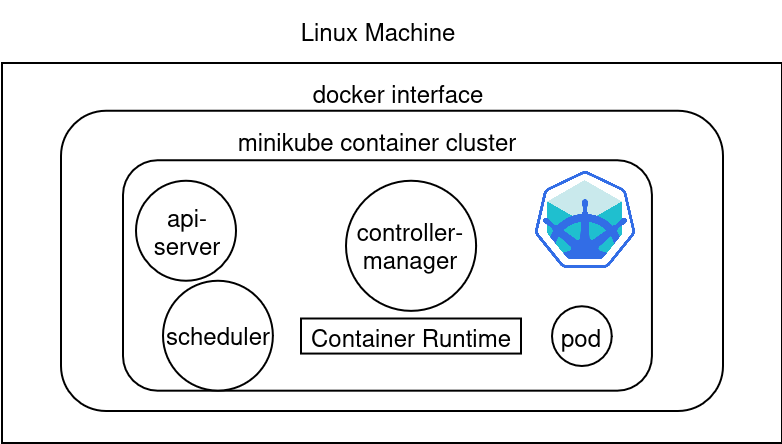
\includegraphics[width=0.9\textwidth]{Design/minikube_driver.png}
\end{figure}
\label{fig:minikube_driver}
Fig~\ref{fig:minikube_driver} illustrates the architecture of Minikube, showing how it can run on various drivers like Docker, VirtualBox, or KVM. It highlights the flexibility of Minikube in adapting to different environments while providing a consistent Kubernetes experience.
Minikube's architecture allows it to run on various drivers like Docker, VirtualBox, or KVM, providing flexibility in how the local cluster is set up. It can also be easily integrated with other tools like Helm for package management and kubectl for command-line operations. Minikube is particularly useful for learning Kubernetes concepts, testing applications, and developing locally before deploying to production clusters.

\subsubsection{kind}
Kind (Kubernetes IN Docker) is a fast and lightweight tool that runs Kubernetes clusters inside Docker containers \cite{kind-docs}. It's designed mainly for testing Kubernetes itself or running automated CI/CD pipelines. Kind is quick to start and destroy, making it ideal for scenarios where clusters need to be recreated often. However, it doesn't provide many built-in add-ons, and setting up networking features like Ingress or LoadBalancer typically needs more manual configuration. Kind is more suitable for automated testing than hands-on experimentation with services or full-featured deployments.

\subsubsection{K3s}
K3s is a lightweight Kubernetes distribution developed by Rancher and optimized for low-resource environments such as edge devices and IoT systems \cite{k3s-docs}. Despite being compact, K3s remains fully Kubernetes-compliant and supports modern features like Helm charts and CRDs. It is often used in production for small clusters, thanks to its low memory usage and simplified installation. While K3s is powerful, it may not be the best starting point for new users due to its minimal abstraction and less emphasis on beginner documentation.

\subsection{Local Clusters Comparison}
\begin{table}[h]
\centering
\begin{tabular}{|l|c|c|c|}
\hline
\textbf{Aspect} & \textbf{Minikube} & \textbf{kind} & \textbf{K3s} \\
\hline
Setup & Easy & Very Easy & Moderate \\
Use Case & Learning / Dev & CI/CD Testing & Edge / IoT \\
Add-ons & Built-in & Manual setup & Limited \\
Performance & Moderate & Fast & Very Lightweight \\
Community & Large & Niche & Growing \\
\hline
\end{tabular}
\caption{Simplified Comparison of Local Kubernetes Clusters}
\end{table}


After comparing all three tools, it was decided to proceed with Minikube for this project. It offers the best balance between usability, features, and support. The wide range of add-ons made it easier to test application deployments, networking policies, and configuration setups. Its clear documentation and active support community also reduces the time spent on troubleshooting. Although kind and K3s are also capable tools, Minikube gave us the flexibility needed to experiment freely in a cost-effective and controlled environment.

ALl of the internal component communication in the local clusters are based in TCP and HTTP 1.1. Neither of the Kubernetes solutions support forwarding QUIC connections natively hence, alternative workarounds are needed.

\subsection{Custom Resource Definitions (CRDs)}
Custom Resource Definitions (CRDs) let users add new types of objects to Kubernetes, such as Gateway API (see section 2.6.10). These custom resources behave like built-in ones, such as Pods, Services, allowing teams to manage them using tools like kubectl. A CRD only defines the structure of a custom resource. To make it work, a separate program called a controller watches for changes and performs actions to match the desired state. Controllers are often built using tools like Kubebuilder or Operator SDK.

CRDs are widely used in tools like Prometheus Operator to automate tasks and manage infrastructure. While building controllers can be complex, they allow teams to create powerful, reusable, and automated workflows inside Kubernetes. In this project, CRDs help manage Apache Pulsar clusters automatically within Kubernetes, making deployment and scaling much easier.

\subsection{Ingress Controllers in Kubernetes}
An Ingress Controller is a critical component in Kubernetes used to expose services, APIs, or web applications running inside the cluster to external users over HTTP or HTTPS. It works alongside Ingress resources, which define routing rules, to manage how external requests reach internal services. While Kubernetes provides the Ingress resource as part of its API, it does not ship with a default controller—users must install and configure one manually. Ingress controllers interpret these rules and handle tasks such as URL-based routing, TLS termination, and load balancing, enabling scalable, declarative web and API access. The different types of ingress controllers are as follows:



For platform-independent or more advanced use cases, several third-party ingress controllers are widely adopted. The NGINX Ingress Controller is the most common, known for its flexibility and ease of use across any Kubernetes setup. Traefik is a modern alternative that auto-discovers services and integrates well into dynamic or CI/CD-heavy environments. For API-first architectures, the Kong Ingress Controller doubles as an API gateway, offering authentication, rate limiting, and monitoring features. Istio's Ingress Gateway, designed for service meshes, provides advanced capabilities like mTLS, circuit breaking, and traffic splitting—ideal for secure, production-grade microservices deployments.

The following is the syntax for ingress controllers
\begin{lstlisting}[language=yaml]
apiVersion: networking.k8s.io/v1
kind: Ingress
metadata:
  name: example-ingress
  annotations:                        # (Controller-specific customizations go here)
    <controller-specific-annotations>
spec:
  ingressClassName: <controller-name>  # (Name of the ingress class, like nginx, alb, kong)
  rules:
  - host: <your-domain.com>
    http:
      paths:
      - path: /                       # (URL path prefix to match)
        pathType: Prefix              # (Usually Prefix or Exact)
        backend:
          service:
            name: <service-name>     # (Your Kubernetes service name)
            port:
              number: <port-number>  # (Service port to route traffic to)
\end{lstlisting}
Here we would use the custom annotations for the specific ingress we will use.


\subsection{Ingress Controller Support for HTTP/3 and QUIC}
HTTP/3, the latest evolution of the HTTP protocol, brings significant advantages in performance and reliability by using QUIC, a transport protocol that operates over UDP and integrates TLS 1.3. Despite growing interest in HTTP/3 for its benefits—such as reduced latency and improved multiplexing—Kubernetes Ingress Controllers have been slow to adopt it due to technical challenges and architectural limitations.

Most widely-used Ingress Controllers, like NGINX and HAProxy, are based on traditional HTTP/1.1 and HTTP/2 over TCP. Since HTTP/3 relies on QUIC, it requires support for UDP, TLS 1.3, and specialized libraries like BoringSSL. These changes involve substantial rewrites of existing proxying logic and networking layers, making native support difficult. As a result, HTTP/3 functionality in Kubernetes Ingress Controllers is generally experimental, requiring custom builds, complex configuration, and lack of standardization across implementations.


\subsubsection{NGINX Ingress Controller and HTTP/3 Support}

NGINX Ingress Controller is one of the most widely adopted ingress controllers in Kubernetes \cite{nginx-ingress-docs}. However, its official support for HTTP/3 remains limited and somewhat unclear. The official NGINX Ingress Controller documentation lacks a straightforward guide for enabling HTTP/3, making configuration challenging for users attempting to adopt this protocol.

At the core, HTTP/3 support in the underlying NGINX web server is provided via the \texttt{ngx\_http\_v3\_module}, which has been available since NGINX version 1.25.0. However, this module is \textbf{not built into the official NGINX package by default}. Enabling HTTP/3 requires compiling NGINX from source with the \texttt{--with-http\_v3\_module} flag and linking it against a QUIC-compatible TLS library such as \textbf{BoringSSL} or \textbf{QuicTLS}. This setup is more feasible at the web server level than within the Kubernetes-managed ingress controller.

To investigate support at the Kubernetes ingress level, attempts were made to pass relevant parameters via Helm during deployment:

\begin{verbatim}
helm install ingress-nginx ingress-nginx/ingress-nginx \
  --namespace ingress-nginx --create-namespace
\end{verbatim}

This opened TCP ports in the service. To enable QUIC support, UDP traffic must also be allowed to reach the ingress. Therefore, the following patch was applied to the service to expose UDP on port 443:

\begin{verbatim}
kubectl patch svc ingress-nginx-controller -n ingress-nginx \
  --type='json' -p='[{"op": "add", "path": "/spec/ports/-", 
  "value": {"name":"quic","port":443,"protocol":"UDP","targetPort":443}}]'
\end{verbatim}

In the latest versions of the NGINX Ingress Controller, the HTTP/3 module appears to be compiled in by default. Additional configurations to expose QUIC via UDP were attempted.

Despite these configurations, the ingress controller does not currently provide sufficient mechanisms to fully inject QUIC and HTTP/3 configuration parameters within a Kubernetes environment, as the NGINX Ingress Controller does not support any specific flags for QUIC behavior. There are \textbf{no officially supported parameters} to manage QUIC-specific settings or negotiate HTTP/3 connections reliably. As a result, while partial support exists at the NGINX core level, the NGINX Ingress Controller's HTTP/3 capabilities remain \textbf{experimental and limited} in practical Kubernetes deployments.



\subsubsection{HAProxy Ingress Controller and HTTP3 Support}
HAProxy has introduced experimental HTTP/3 support starting with version 2.6 \cite{haproxy-docs} \cite{haproxy-k8s-docs}. Its Ingress Controller can leverage this functionality. This includes enabling UDP listeners, tuning TLS settings, and adjusting protocol stacks manually—none of which are typically available through standard Helm charts. 


To test HTTP/3 support in a Kubernetes environment, the following steps were performed:

\begin{enumerate}
  \item The HAProxy Helm repository was added and updated:
  \begin{verbatim}
  helm repo add haproxytech https://haproxytech.github.io/helm-charts
  helm repo update
  \end{verbatim}

  \item The HAProxy ingress controller was installed with a custom values file:
  \begin{verbatim}
  helm install haproxy-quic haproxytech/kubernetes-ingress -f haproxy-quic-values.yaml
  \end{verbatim}

  In the \texttt{haproxy-quic-values.yaml} file, the configuration exposed UDP port 443 and passed the flag \texttt{--quic-bind-port=443} to enable QUIC and HTTP/3 support.

  \item An \texttt{Ingress} resource was applied, using the HAProxy ingress class and pointing to a backend service. A self-signed TLS certificate was used with the hostname \texttt{quic-aioquic.com}.
\end{enumerate}

Once deployed, HTTP/3 functionality was tested using \texttt{curl}:

\begin{verbatim}
curl --http3-only --verbose --insecure https://192.168.49.4 \
  -H "Host: quic-aioquic.com"
\end{verbatim}

The response confirmed that HTTP/3 was successfully negotiated. However, backend service logs indicated that the request was received using HTTP/1.1:

\begin{verbatim}
10.244.1.122 - - [07/Aug/2025:12:55:39 +0000] "GET / HTTP/1.1" ...
\end{verbatim}

This confirms that HAProxy terminates the HTTP/3 connection and opens a new one to the backend using a lower protocol version.

\paragraph{Limitations.}
Although HAProxy can accept HTTP/3 connections from clients, it does not forward them using HTTP/3 to backend services. The ingress controller does not support inspecting or demultiplexing QUIC packets. As a result, HTTP/3 is only supported at the edge, and end-to-end HTTP/3 communication within Kubernetes is not yet feasible using HAProxy.



\subsubsection{Workarounds}
Given the lack of mature, native HTTP/3 support in mainstream Ingress Controllers, it is currently more practical to experiment with HTTP/3 directly at the web server level for Nginx and Traefic which wasnt able to support ingress like ha-proxy. We will look at the webserber Angie which is a fork of nginx especially created for h3 support in section

\subsection{Gateway API}
\subsubsection{Overview}
The Gateway API is a recent advancement in Kubernetes networking designed to address the limitations of the traditional Ingress API. While Ingress has served as the de facto method for managing external traffic into Kubernetes clusters, it suffers from inflexibility, heavy reliance on annotations, and poor support for non-HTTP protocols. The Gateway API introduces a more robust, extensible, and protocol-agnostic model that allows infrastructure operators and application developers to define their concerns independently, thus supporting multi-tenancy and complex networking scenarios more effectively.

One of the defining features of the Gateway API is its emphasis on supporting a wide variety of protocols beyond HTTP and HTTPS, such as TCP and UDP, with emerging support for QUIC and HTTP/3. This makes the API particularly relevant for modern, low-latency, and multiplexed applications that demand richer transport capabilities. The architecture facilitates this through a set of Kubernetes-native Custom Resource Definitions (CRDs), allowing developers and operators to interact with networking policies declaratively and with clear separation of responsibilities.


\subsubsection{Architecture and Core Components}
The Gateway API introduces modular CRDs for fine-grained network traffic control in Kubernetes. GatewayClass defines types of gateways, such as Envoy, HAProxy, managed by admins, while Gateway instances configure ports, protocols, and TLS settings. Routing is handled by resources like HTTPRoute, TCPRoute, and UDPRoute, which forward traffic based on specific rules. Additional resources like ReferencePolicy support cross-namespace and security configurations. This design separates infrastructure and application concerns, improving scalability, security, and maintainability


\subsubsection{Gateway API Implementation for HTTP3 Support}

Since HAProxy successfully worked with Ingress for HTTP/3 forwarding, the next step was to implement the Gateway API using the HAProxy controller.

\subsubsubsection{Installing the HAProxy Gateway Controller}

The following steps were performed:

\begin{itemize}
  \item Added the Helm repository:
\begin{lstlisting}[language=bash]
helm repo add haproxytech https://haproxytech.github.io/helm-charts
helm repo update
\end{lstlisting}

  \item Installed the controller with Gateway API support:
\begin{lstlisting}[language=bash]
helm install haproxy-gateway-controller haproxytech/kubernetes-ingress \
  --namespace haproxy-gateway-system --create-namespace \
  --set controller.kubernetesGateway.enabled=true \
  --set controller.kubernetesGateway.gatewayControllerName=haproxy.org/gateway-controller \
  --set controller.service.type=LoadBalancer
\end{lstlisting}
\end{itemize}

Once deployed, a LoadBalancer service was exposed, including a UDP port for QUIC:

\begin{lstlisting}[language=bash]
NAME                                            TYPE           CLUSTER-IP     EXTERNAL-IP    PORT(S)                                                                  AGE
haproxy-gateway-controller-kubernetes-ingress   LoadBalancer   10.104.20.31   192.168.49.5   80:31433/TCP,443:32261/TCP,443:32261/UDP,1024:30450/TCP,6060:31286/TCP   117s
\end{lstlisting}

\subsubsection{Defining the Gateway}

The Gateway resource was created to expose HTTPS and QUIC traffic:

\begin{lstlisting}[language=yaml]
apiVersion: gateway.networking.k8s.io/v1
kind: Gateway
metadata:
  name: haproxy-gateway
spec:
  gatewayClassName: haproxy
  listeners:
  - name: https
    protocol: HTTPS
    port: 443
    tls:
      mode: Terminate
      certificateRefs:
      - kind: Secret
        name: your-tls-secret
  - name: quic
    protocol: HTTPS
    port: 443
    tls:
      mode: Terminate
      certificateRefs:
      - kind: Secret
        name: your-tls-secret
\end{lstlisting}

\subsubsection{Defining the HTTPRoute}

An HTTPRoute was defined to route requests based on hostname:

\begin{lstlisting}[language=yaml]
apiVersion: gateway.networking.k8s.io/v1
kind: HTTPRoute
metadata:
  name: haproxy-http3-route
spec:
  parentRefs:
  - name: haproxy-gateway
    sectionName: https-quic
  hostnames:
  - "gateway-haproxy.com"
  rules:
  - backendRefs:
    - name: http3-test
      port: 80
\end{lstlisting}

\subsubsection{Packet Flow Description}

The observed packet flow is as follows:

\begin{itemize}
  \item Client sends request to LoadBalancer service.
  \item The HAProxy pod receives the request, decrypts it using the TLS certificate.
  \item It matches the hostname and routes the request based on the Gateway and Route configuration.
  \item The request is forwarded to the backend service.
\end{itemize}

\subsubsection{Operational Separation}

The Gateway API introduces a clean separation of responsibilities:
\begin{itemize}
  \item \textbf{Infrastructure providers} manage the GatewayClass resources, such as HAProxy, NGINX.
  \item \textbf{Cluster administrators} handle gateway resources, such as TLS, listeners, ports.
  \item \textbf{Application developers} define HTTPRoute or TCPRoute objects, configuring hostnames and routing rules.
\end{itemize}

This separation encourages better scalability and maintainability in Kubernetes environments.

\subsubsection{Observed Limitation in HTTP/3 Stream Handling}

While the Gateway API supports HTTP/3 and correctly forwards such requests to backend services, a limitation was observed:

When HTTP/3 requests are made, the Gateway forwards them correctly, showing basic QUIC support. However, similar to the behavior of the HAProxy Ingress Controller, the Gateway API treats the request as a single unit. There is no visibility or control over individual HTTP/3 streams.

This indicates that the Gateway API currently lacks support for stream-level features of HTTP/3. It does not provide insight into or allow manipulation of separate streams within a connection. Therefore, the full capabilities of HTTP/3, such as fine-grained stream-level routing or observation, are not realized.

\subsubsection{Declarative Configuration vs. Annotation-Driven Models}
A major improvement introduced by the Gateway API is its declarative configuration model, which replaces the annotation-heavy approach of the traditional Ingress API. Annotations in Ingress controllers often lack standardization, are implementation-specific, and are difficult to validate, leading to operational ambiguity. In contrast, the Gateway API uses structured CRDs to define listeners, routes, and policies, making configuration clearer, more consistent, and easier to validate.

Nevertheless, annotations have not been entirely eliminated. They are still used in specific cases, particularly to enable experimental features or for backward compatibility with legacy tooling. For example, enabling QUIC support or selecting specific cipher suites via BoringSSL may still require annotations, depending on the controller. However, these annotations are supplementary rather than central, with the primary configuration expressed through first-class Kubernetes resources. This allows for richer multi-protocol configurations—such as defining a single gateway that supports both TCPRoute and UDPRoute—an arrangement difficult to express using traditional Ingress.


\subsection{QUIC Library Implementations}
The standardization of the QUIC protocol by the IETF has encouraged the development of several independent and open-source implementations to support integration across diverse ecosystems. These implementations serve not only as vehicles for QUIC protocol adoption but also as platforms for experimentation, optimization, and integration into real-world systems. Among the most prominent and actively maintained QUIC libraries are Aioquic, Quic-go, and Quiche, each developed in a distinct programming language and suited to particular performance and deployment goals. This section provides a detailed examination of these libraries, discussing their internal architecture, design philosophies, and practical usage in production or research environments.

\subsubsection{Aioquic}
Aioquic is a Python-based implementation of the QUIC and HTTP/3 protocols developed by aiortc, and is designed to provide asynchronous, non-blocking I/O through Python's asyncio framework. Aioquic is particularly well-suited to academic and research applications due to its readability, high-level abstractions, and ease of integration within Python-based systems. It supports essential QUIC features such as stream multiplexing, TLS 1.3 handshake, connection migration, datagram frames, 0-RTT resumption, and HTTP/3 protocol negotiation.

\paragraph{Architecture and Design}
At the core of Aioquic lies an event-driven state machine that responds to received packets and timer expirations. It integrates closely with Python's asyncio event loop, allowing developers to implement clients and servers that handle concurrent connections efficiently using coroutines. The QuicConnection class encapsulates the transport logic, while the H3Connection class manages the HTTP/3 layer on top of QUIC streams. Developers can subclass the QuicConnectionProtocol to customize behavior for server-side or client-side implementations.

Aioquic also includes built-in support for logging using qlog, a standardized QUIC tracing format. This enhances its suitability for debugging and protocol analysis. In terms of modularity, the library is structured to allow developers to use just the QUIC transport layer or to integrate HTTP/3 as needed, making it flexible for building custom protocols atop QUIC.

\paragraph{Implementation Example}
A typical Aioquic application involves initializing a QUIC configuration, creating a connection context, and using asynchronous tasks to send and receive data. Below is a simplified example of a client establishing a secure QUIC connection and sending data over a stream:

\begin{lstlisting}[language=python]
from aioquic.asyncio import connect
from aioquic.quic.configuration import QuicConfiguration
import asyncio

async def main():
    configuration = QuicConfiguration(is_client=True)
    async with connect("example.com", 4433, configuration=configuration) as protocol:
        stream_id = protocol._quic.get_next_available_stream_id()
        protocol._quic.send_stream_data(stream_id, b"Hello, QUIC!", end_stream=True)
        await protocol.wait_closed()

asyncio.run(main())
\end{lstlisting}

This minimal example illustrates Aioquic's ease of use and is indicative of how rapidly developers can prototype with the library.

\paragraph{Use Cases and Adoption}
While Aioquic is not yet widely deployed in commercial production environments due to Python's performance limitations, it is frequently used in academic research, protocol testing, and rapid prototyping.

\subsubsection{Quic-go}
Quic-go is a Go-based implementation of the QUIC protocol, maintained by the open-source community and initially developed by lucas-clemente, with substantial contributions from the Chromium networking team. Quic-go is designed for robustness and performance and has been widely integrated into real-world systems, including browsers and cloud-native applications.

\paragraph{Architecture and Design}
Quic-go leverages Go's lightweight concurrency model through goroutines and channels, making it highly scalable for managing thousands of concurrent QUIC sessions. The library adheres closely to the IETF QUIC specification and includes a complete implementation of HTTP/3, along with transport features such as packet pacing, congestion control, such as CUBIC, BBR, retransmissions, connection ID rotation, stateless resets, and forward error correction.

The internal architecture comprises multiple interacting subsystems: the connection package manages connection-level state, streams handles stream multiplexing, and ackhandler is responsible for packet acknowledgment and retransmission tracking. The integration of Go's cryptographic primitives allows native handling of TLS 1.3 through the crypto/tls library.

\paragraph{Implementation Example}
The following snippet illustrates a basic QUIC server using Quic-go, which listens for incoming connections and echoes received data:

\begin{lstlisting}[language=go]
package main

import (
    "crypto/tls"
    "github.com/quic-go/quic-go"
    "io"
    "log"
)

func main() {
    tlsConf := &tls.Config{
        Certificates: []tls.Certificate{loadTLSCertificate()},
        NextProtos:   []string{"h3"},
    }

    listener, err := quic.ListenAddr(":4242", tlsConf, nil)
    if err != nil {
        log.Fatal(err)
    }

    for {
        sess, err := listener.Accept(nil)
        if err != nil {
            log.Fatal(err)
        }
        go handleSession(sess)
    }
}

func handleSession(sess quic.Connection) {
    stream, err := sess.AcceptStream(nil)
    if err != nil {
        log.Println(err)
        return
    }
    io.Copy(stream, stream) // Echo
}
\end{lstlisting}

This example demonstrates how Quic-go abstracts away low-level networking concerns, allowing developers to focus on application logic.

\paragraph{Use Cases and Adoption}
Quic-go is embedded in the Chromium browser stack, where it underpins HTTP/3 communication. It has also been adopted in several high-throughput applications, including Caddy, a modern Go-based web server, and FrankenQUIC, a QUIC protocol experimentation platform. Its production-readiness and active maintenance make it an excellent choice for developers building scalable, network-intensive applications in the Go ecosystem.

\subsubsection{Quiche}
Quiche is a QUIC and HTTP/3 implementation written in Rust by Cloudflare, focusing on performance, security, and integration into high-speed, production-grade systems. Quiche is used extensively within Cloudflare's global CDN infrastructure, where it handles millions of QUIC connections across edge locations.

\paragraph{Architecture and Design}
Quiche benefits from Rust's safety guarantees and zero-cost abstractions, which make it ideal for low-level network programming. The library is designed to operate as a "no-std" Rust crate, enabling usage in environments with limited standard library support - such as embedded systems or unikernels.

The architecture revolves around a stateful Connection object, which manages packet parsing, stream states, congestion control, and cryptographic negotiation. The library implements advanced features such as 0-RTT data resumption, QPACK header compression, packet coalescing, and stream prioritization. Quiche also offers tight integration with qlog tracing and supports ALPN negotiation for HTTP/3 and custom application protocols.

Quiche is built to be embedded into other C/C++/Rust programs via its Foreign Function Interface (FFI), making it highly versatile.

\paragraph{Implementation Example}
A basic HTTP/3 server using Quiche is more complex due to Rust's strict safety model, but the following pseudocode outlines the core flow:

\begin{lstlisting}[language=rust]
let mut conn = quiche::accept(&scid, None, local_addr, peer_addr, &mut config)?;
let (read, _) = socket.recv_from(&mut buf)?;
let recv_info = quiche::RecvInfo { from: peer_addr, to: local_addr };

conn.recv(&mut buf[..read], recv_info)?;

if conn.is_established() {
    if let Ok((stream_id, data)) = conn.readable().next() {
        // Process stream data
    }
}
\end{lstlisting}

This example shows the control developers have over connection handling and packet flow when using Quiche.

\paragraph{Use Cases and Adoption}
Quiche is used in Cloudflare's HTTP/3 infrastructure and has been integrated into major projects such as Nginx, curl, and Wireshark (for traffic analysis). Its adoption by performance-critical applications highlights its production maturity and scalability. Additionally, its inclusion in the QUIC Interop Runner and extensive qlog support make it a valuable reference implementation for QUIC protocol conformance testing.

\subsubsection{Summary of Libraries}
The three libraries—Aioquic \cite{aioquic-repo}, Quic-go \cite{quic-go-repo}, and Quiche \cite{quiche-repo} explains the diversity of QUIC implementations, each targeting different domains. Aioquic prioritizes accessibility and research flexibility whereas Quic-go balances performance and developer usability and finally Quiche focuses on high-throughput, secure, production deployments. The choice among them depends on the development environment, performance constraints, and programming language expertise. In the context of this dissertation, Aioquic is selected for the implementation phase because of its easy syntax.  ie. Python being easy to understand and configure.

\subsection{Angie Webserver}
Angie is a high-performance, modular web server and reverse proxy developed as a fork of NGINX, with explicit focus on supporting emerging protocols and modern web traffic patterns \cite{angie-docs}. One of Angie's key differentiators is its support for HTTP/3 via native QUIC integration. By leveraging QUIC, Angie can handle low-latency, multiplexed connections over UDP, making it suitable for next-generation web workloads. Angie's modular architecture also facilitates extensibility for protocol enhancements and security mechanisms.

In this study, Angie was deployed within a Kubernetes environment using the official container image (docker.angie.software/angie:latest). Configuration was managed via a Kubernetes ConfigMap, specifying server blocks, TLS settings, and QUIC-related directives. Angie successfully forwarded HTTP/3 traffic to backend services, validating its compatibility with QUIC at the connection level. However, its current implementation lacks the ability to perform stream-level inspection or manipulation within QUIC connections. This limits its support for finer-grained traffic control and observability across individual HTTP/3 streams in production environments.

Despite these limitations, Angie presents a stable and efficient reverse proxy solution for HTTP/3 traffic, suitable for experimental deployments and scenarios where basic QUIC forwarding suffices. Its adherence to evolving protocol standards and active development trajectory make it a compelling candidate for future-ready capable proxy.

\subsubsection{Angie Configuration for HTTP/3 Forwarding}
Angie's architecture supports HTTP/3 by enabling QUIC listeners alongside traditional TCP listeners. The proxy was deployed Angie using the Docker image docker.angie.software/angie:latest in a Kubernetes environment, configured via a ConfigMap as shown below:

\begin{lstlisting}[language=yaml]
apiVersion: v1
kind: ConfigMap
metadata:
  name: angie-config
data:
  angie.conf: |
    worker_processes auto;
    events {}
    http {
      log_format detailed '$remote_addr - $remote_user [$time_local] '
                          '"$request" $status $body_bytes_sent '
                          '"$http_referer" "$http_user_agent" '
                          'protocol=$server_protocol http3=$http3';
      access_log /dev/stdout detailed;
      server {
        listen 443 ssl;
        listen 443 quic reuseport;
        ssl_certificate     /certs/tls.crt;
        ssl_certificate_key /certs/tls.key;
        add_header Alt-Svc 'h3=":443"; ma=86400; persist=1';
        ssl_protocols TLSv1.3;
        ssl_ciphers HIGH:!aNULL:!MD5;
        ssl_prefer_server_ciphers on;
        http2 on;
        location / {
          return 200 "Hello from Angie via HTTP/3!\n";
        }
        location /service {
          proxy_pass https://quic-service.default.svc.cluster.local;
        }
        location /pod {
          proxy_http_version 3;
          proxy_pass https://quic-service.default.svc.cluster.local;
        }
        location /test-h3 {
          add_header X-Test-Protocol $server_protocol;
          add_header X-Test-Http3 $http3;
          return 200 "This is /test-h3 (HTTP version: $server_protocol, http3: $http3)\n";
        }
      }
    }
\end{lstlisting}

This configuration enables Angie to listen for QUIC traffic on port 443 (listen 443 quic reuseport), advertise HTTP/3 support via the Alt-Svc header, and forward requests to a backend service (quic-service.default.svc.cluster.local) using HTTP/3 (proxy\_http\_version 3). The Kubernetes Deployment and Service manifests further expose Angie as a LoadBalancer, supporting both TCP and UDP traffic on port 443.
This allows it to proxy http3 traffic to backend but faces the same limitation as faced in haproxy ingress controller and gateway api of not having stream level knowledge

\subsection{Limitation of Modern Webservers for H3 Support}
A fundamental limitation observed in both Angie web server is the inability to perform stream-level inspection of QUIC traffic. QUIC, by design, supports stream multiplexing, which allows multiple concurrent and independent streams—such as HTML documents, images, or scripts—to be transmitted over a single connection without head-of-line blocking. However, both Angie and other webservers treat QUIC packets as udp datagrams and do not parse or prioritize individual streams.

This architectural constraint significantly limits their ability to apply intelligent routing, prioritization, or filtering at the stream level. No granular control over the constituent streams and no existing mechanisms existing to allow such modification raises a critical problem. 

Consequently, while reverse proxies, ingresses and gateway api support the transport of HTTP/3 traffic, they do not fully exploit QUIC's stream-level features, which restricts their applicability in more advanced use cases such as fine-grained traffic management or application-aware routing.

\subsection{Load Balancers for HTTP/3 Traffic Management}
\subsubsection{Overview}
Load balancers are critical components in modern distributed systems, enabling traffic distribution across backend services to ensure scalability, fault tolerance, and availability. With the rise of HTTP/3, which operates over the QUIC protocol and utilizes UDP, load balancers must evolve to support this shift from traditional TCP-based communication.

Service load balancers distribute incoming network traffic across multiple backend servers, optimizing resource utilization and ensuring fault tolerance. In Kubernetes, the Service resource with a LoadBalancer type exposes applications externally, typically integrating with cloud provider load balancers in cloud environments or requiring alternative solutions in on-premises setups. The adoption of HTTP/3, built atop QUIC, requires load balancers to support UDP traffic, as QUIC's low-latency handshake and stream multiplexing rely on UDP datagrams rather than TCP.


\subsubsection{MetalLB for On-Premises Load Balancing}
MetalLB is a lightweight, open-source load balancer specifically designed for bare-metal Kubernetes clusters that do not rely on cloud providers \cite{metallb-docs}. It supports both TCP and UDP traffic and integrates seamlessly with Kubernetes via the LoadBalancer service type. In this solution, MetalLB is used to expose HTTP/3 services externally by assigning static IPs from a pre-defined pool. Once configured, it enables Minikube to accept external HTTP/3 connections over port 443, acting as the ingress point to the cluster for QUIC-based traffic. This makes it a practical choice for on-premises testing and development of HTTP/3 applications.

\subsubsection{Challenges of MetalLB}
While MetalLB fulfills the basic requirement of enabling UDP passthrough for HTTP/3 traffic, it does not provide advanced capabilities seen in cloud load balancers. It cannot inspect individual QUIC streams, meaning it treats all QUIC packets as udp datagrams and lacks stream-level routing or prioritization. It also lacks features such as autoscaling, failover, and built-in redundancy, which are critical for production-grade environments. Configuration in metal-lb must be done manually, including the setup of IP address pools and service manifests. MetalLB's compatibility with Minikube makes it suitable for local HTTP/3 testing, where external access and QUIC packet forwarding are necessary but enterprise grade production features are not.

\subsection{Apache Pulsar for Streaming Use Cases}
\subsubsection{Introduction to Streaming Systems}
In order to work with modern transport protocols such as QUIC and WebTransport, which support bi-directional, low-latency, and multiplexed data transmission, a streaming use case is typically required. These protocols are specifically designed to operate within systems that continuously process data in motion, rather than in static batches. In the context of modern data-driven architectures, streaming systems have thus become foundational to processing high-velocity, continuous data flows in near real-time. Such systems facilitate the ingestion, transformation, and delivery of data as it is generated, supporting critical use cases including real-time analytics, fraud detection, anomaly monitoring, telemetry processing, and event-driven microservices [Kreps et al., 2011]. At the core of these platforms lies a robust messaging infrastructure, which guarantees the reliable delivery and persistence of events between producers and consumers, enabling scalable and responsive data pipelines.

Two prominent distributed messaging systems supporting streaming workloads are Apache Kafka and Apache Pulsar. While Kafka has historically dominated the event streaming landscape, Apache Pulsar presents a rearchitected solution that addresses several of Kafka's limitations, particularly with respect to scalability, multi-tenancy, and storage management.

\subsubsection{Comparative Evaluation: Apache Kafka vs Apache Pulsar}
Apache Kafka and Apache Pulsar are two leading platforms for distributed event streaming, but they differ significantly in architecture and operational capabilities. Kafka adopts a monolithic design where each broker handles both message processing and local storage. This simplifies the system under certain conditions but introduces limitations in scalability, multi-tenancy, and storage flexibility. Kafka's tight coupling of compute and storage means both must be scaled together, increasing operational overhead.

In contrast, Apache Pulsar follows a cloud-native layered architecture, separating compute (stateless brokers) from storage (Apache BookKeeper). This decoupling allows independent scaling, built-in multi-tenancy, native tiered storage, and geo-replication—features that better support modern, dynamic, and multi-tenant workloads. Pulsar's architecture is particularly aligned with containerized environments and streaming use cases involving QUIC/WebTransport, which require persistent, low-latency streams and decoupled resource management.

Thus, while Kafka remains effective for stable, centralized deployments, Pulsar offers greater architectural flexibility and operational efficiency for contemporary streaming systems. The storage-compute separation gives Pulsar an elastic stability and long-term message retention.

\subsubsection{Apache Pulsar Architecture and Components}
Apache Pulsar's design consists of several modular components, each performing a specific function within the messaging and storage lifecycle. These components collaborate to deliver a scalable, fault-tolerant, and flexible streaming platform.

\paragraph{Pulsar Brokers}
Pulsar brokers are stateless services responsible for handling client requests, maintaining topic metadata caches, and managing the coordination of message dispatch between producers and consumers. Brokers do not store message data locally. Instead, upon receiving a message, a broker writes it to BookKeeper and returns acknowledgements once the required replication factor is achieved.

This stateless nature allows brokers to scale horizontally with minimal coordination overhead. It also enhances system reliability, as brokers can fail and recover without requiring data rebalancing. In streaming scenarios—such as telemetry ingestion, application monitoring, and order processing pipelines—Pulsar brokers facilitate consistent and low-latency message routing across topics.

\paragraph{Apache BookKeeper (Bookies)}
Apache BookKeeper serves as the storage backend for Pulsar and is comprised of nodes referred to as "bookies." Data in Pulsar is persisted in write-ahead log structures called ledgers, which are divided into segments and distributed across multiple bookies. Each segment is replicated (typically across three nodes) for durability and fault tolerance.

BookKeeper enables Pulsar to support high-throughput writes and provides deterministic data placement. Additionally, tiered storage mechanisms allow the migration of older data to cheaper storage backends, such as Amazon S3 or Hadoop-compatible file systems. This makes Pulsar particularly effective for long-term event retention and replay, common in systems involving historical trend analysis or data backfills.

\paragraph{Apache ZooKeeper}
ZooKeeper \cite{zookeeper-docs} is used by Pulsar to coordinate metadata operations, including broker and bookie membership, topic partition assignments, and ledger metadata. It ensures consistency in cluster-wide operations and supports automatic leader election and failover scenarios.

Though newer Pulsar versions aim to decouple from ZooKeeper via alternative metadata stores like Oxia, ZooKeeper remains a critical component in most production deployments. In multi-tenant streaming environments, ZooKeeper facilitates dynamic topic creation and fine-grained resource control across tenants and namespaces.

\paragraph{Pulsar Proxy (Optional)}
The Pulsar Proxy is an optional stateless component that acts as a reverse proxy between clients and brokers. It is particularly useful in cloud-native environments or scenarios involving network segmentation, where direct broker exposure is undesirable. The proxy simplifies client connectivity by routing traffic to the correct broker and is commonly integrated with Kubernetes load balancers, such as MetalLB or Ingress controllers, to expose HTTP or gRPC endpoints.

\paragraph{Pulsar Functions}
Pulsar Functions is a built-in lightweight serverless framework for stream processing. Developers can implement custom logic in Python, Java, or Go and deploy it directly into the Pulsar ecosystem without managing external processing infrastructure. Use cases include real-time filtering, transformation, enrichment, and aggregation of messages.

Unlike Kafka Streams, which requires additional compute resources and cluster management, Pulsar Functions operate within the broker environment, offering simplified deployments for low-latency stream operations.

\subsubsection{Challenges}
Running Pulsar in a local environment is somewhat complex as it requires management of multiple logically separated brokers and bookies, adding configuration challenges. Also, running it in Kubernetes brings challenges for exposing endpoints for brokers. These are addressed in detail in the implementation section.

\subsection{Conclusion}
The state-of-the-art review highlights significant advancements in real-time communication protocols, container orchestration platforms, and scalable streaming architectures that collectively enable next-generation data-driven applications. WebTransport, leveraging the QUIC protocol, marks a substantial leap forward by providing low-latency, multiplexed, and reliable data streams over the web. Its support for both reliable and unreliable transport modes, coupled with connection migration and efficient congestion control, addresses critical challenges faced by interactive applications such as gaming, video conferencing, and telemetry systems.

Kubernetes, as the premier container orchestration framework, is progressively adapting to the demands of these modern protocols. Despite its inherent robustness, Kubernetes faces challenges in seamlessly integrating UDP-based protocols like QUIC and enabling HTTP/3 traffic, which necessitate novel solutions in load balancing, ingress management, and service discovery. Emerging standards such as the Gateway API and custom resource definitions offer promising avenues to enhance Kubernetes' native support, though practical implementations of these protocols in production environments remains a challenge and an active area of research and development.

In the domain of streaming platforms, Apache Pulsar represents a paradigm shift by decoupling compute from storage, in contrast to the traditional monolithic architecture exemplified by Apache Kafka. This architectural innovation affords Pulsar superior scalability, elasticity, and multi-tenancy capabilities, making it particularly well-suited for complex, cloud-native streaming use cases. Pulsar's design aligns closely with the requirements of modern real-time data processing, including those facilitated by WebTransport and QUIC, where high throughput, fault tolerance, and geo-replication are critical.

Looking forward, the integration of WebTransport with Kubernetes and Apache Pulsar presents a direction for building resilient, high-performance streaming systems. Experimental implementations focusing on these technologies will be essential to validate their interoperability, measure performance gains, and address operational challenges. This research is a good way to improve how we build fast, scalable streaming systems for future real-time applications.


% \chapter{Problem Formulation}
% \label{chap:ProblemFormulation}

% The previous chapter described the literature that contributed towards the support of Proxying Quic streams within kubernetes cluster. It summarized the drawbacks of several different approaches and clearly identified the limitations for the approaches by defininig the gaps of the those approaches. Clearly there is a need to be able to have a solution that enables proxying QUIC streams into kubernetes. In other words, there exists a requirement to distribute and loadbalance http3 multiplexed streams within kubernetes. This chapter focuses on correctly identifying the challenges and clearly stating out the gaps occuring in the traditional proxy servers with regards to supporting webtransport streams. This chapter then proceeds to provide a primary approach for this dissertation in order to realise our end result. This chapter starts by giving an abstracted view of the approach that would solve the problem and arrive at a working solution. The next section talks about the novelty of the proposed approach and how it is different from existing working directions. The section covers the idea on the on the intuition behind chosing the approach following which the targets to be achieved for the stated problem are stated. Finally, the identified challenges are listed for the proposed approach.

% \section{Abstracted View of the solution}
% The main objective of this study is to enable Webtransport independent multiplexed streams to be proxied to different microservices in kubernetes envirnoment. This study aims to provide a complete discrete solution to the problem and solving the core problem which other studies did not solve. In order to arrive at a working solution at a highly abstracted way is to find a way to create a kuberentes supported http3 streams based proxy server.

% \begin{table}[H]
% \centering
% \caption{Abstracted View of Proposed Solution}
% \begin{tabular}{|p{4cm}|p{5.5cm}|p{5.5cm}|}
% \hline
% \textbf{Capability Area} & \textbf{Existing Approaches} & \textbf{Our Approach (Custom Proxy Server)} \\
% \hline
% Stream Visibility & Operate at packet level with no awareness of streams & Enable deep stream-level visibility and context recognition \\
% \hline
% Stream Handling & Entire connection treated as a monolithic flow & Demultiplex and manage streams individually \\
% \hline
% Application-Layer Intelligence & Minimal application-layer insight or control & Enable content-based routing, security, and monitoring per stream \\
% \hline
% \end{tabular}
% \end{table}


% \section{Differences from existing approaches}
% As stated in the previous chapter most of the existing approaches do not address the problem at hand which is independent stream level inspection and control. Most of the approaches use custom annotations in ingress or use third party libraries but finally ends up routing entire UDP packet when it comes to http3 streams to the server. On the other hand work for this specific problem is currently in progress and is being addressed but there has not yet been a working solution which addresses the core problem. Thus, our apporach differs in a way that modification are done to the working quic library implementation to make a progress towards creating a standardized solution. The difference in approaches is shown in the table below





% This section should present a short review of the topics discussed in the State of the Art chapter in order to then discuss gaps in the existing work and the relationship of these gaps to the work described in this dissertation.

% \section{Proposed Work}
% % This section should provide a thorough description of the problem and an overview of the
% % work proposed to address the problem.
% To cater to the problem of Head of the line blocking with TCP, Quic Protocol was incepted and formalized. With Quic streams we are able to leverage the performance benefit only if one can use it at scale. Kubernetes is the state of the art modern solution for deploying applications in containers across multiple machines as microservices and there exists gaps witth regard to the support of quic streams hindering being able to leverage the capability of http3 webtransport streams.  Current solutions in kubernetes does not act as stream forwards but rather act as UDP packet forwarders as they operate at a lower level abstraction rather than providing granular application level visibility. Kubernetes environment is largely based on TCP and Http 1.1 Protocols and support for Http3 streams is not natively support by any Kubernetes objects. The approach to the the solution is addressing the gaps individually. To first address the lack of support by native kuberentes objects the proposed solution would be expected to be deployed as a Pod exposed via service in kubernetes. To address the solution, a custom proxy server supporting acceptance of webtransport streams is proposed. To demonstrate the working prototype a streaming usecase is used along with widely used streaming tools. This approach addresses the problem at hand and provides a suitable working solution/


% Defining the chapter
\chapter{Problem Formulation}

In this chapter, the research problem of this dissertation is determined as the problem of combining modern WebTransport over QUIC protocol \cite{rfc9000} with Kubernetes \cite{kubernetes-docs}. WebTransport \cite{webtransport-draft}, QUIC, Kubernetes are very sophisticated technologies, and integrating the 3 technologies to provide real-time and low latency applications is challenging. This chapter addresses the research gaps based on the State of the Art with additional aspects of it and proposes a new solution to these problems and a clear plan to solve. It also discusses the difference between the proposed methodology and the current methods and provides certain design and implementation objectives in order to obtain a sustainable, production-ready streaming framework.

This chapter effectively explains the problem it wants to address, offers an abstracted solution, tells how the work is different among other solutions and provides a blueprint on how the designed solutions could be attained.

% Section 3.1: Identified Challenges
\section{Identified Challenges}
The State of the Art review highlights that there is substantial advancement in modern transport protocols, cloud-based networking as well as streaming platforms. But it also highlights the issues that act against formation of high-performance and real-time systems in kubernetes. The need to conduct this research is motivated by the following challenges, some of which are briefly explained below.

\subsection{Limited Support for QUIC and HTTP/3 in Kubernetes Ingress Controllers}
Experimental QUIC and HTTP/3 support have been added to Kubernetes Ingress Controllers such as NGINX, HAProxy, and Envoy via controller specific annotations such as \ct{nginx.org/quic: \textquotesingleysis true\ila Spaging (Section 2.6.9.4). Nevertheless, such implementations are unreliable and not production ready. Nginx Controller currently does not support proxying and HAProxy fails to proxy streams. The Gateway API has a more open model, and allows protocols that use UDP such as QUIC (Section 2.6.10.3), and its utility relies on the capabilities of underlying reverse proxies.

Moreover, proxies like Angie and HAProxy along with the ingress controller cannot inspect or manage individual QUIC streams (Sections 2.6.12, 2.6.13, 2.6.14). This limitation prevents features like stream-aware routing, prioritization, etc which are essential for low-latency applications such as real-time streaming or telemetry. As a result, building efficient, stream-aware systems in Kubernetes remains a challenge.

\subsection{Challenges in Load Balancing for QUIC-Based Traffic}
Unlike the traditional TCP-based protocols, QUIC uses UDP, so it becomes a challenge in Kubernetes environments where the traffic is heavily built on TCP traffic. The cloud service providers, such as Google Cloud, has already implemented support of QUIC in their load balancers with protocol downgrade, whereas on-premise load balancer implementations (such as MetalLB) do not have advanced features such as supporting stream-level routing, autoscaling, or failover (Section 2.6.15.4). Metal-lb doesnt support quic proxying and treats http as UDP packets. This creates a challenge in managing QUIC-based traffic in a cluster, which is on-prem, local or privately owned, thus encapsulating the scalability of HTTP/3 applications.


\subsection{Operational Complexity and Observability}

QUIC’s encrypted headers and multiplexed streams in QUIC improve performance and security at the expense of making traffic inspection difficult. Kubernetes environment being largely based on tcp have weak weak support for QUIC, which makes it harder to debug and analyze performance (Section 2.6.10.6). Even the Gateway API decouples infrastructure and application considerations, a misconfiguration of work makes whole operation within kubernetes more difficult (Section 2.6.10.6). These issues create barriers to building reliable, real-time webtransport stream demultiplexers/Routers in kubernetes.

% Section 3.2: Abstracted View of the Solution
\section{Abstracted View of the Solution}


The aim of this dissertation is to open a possibility of allowing independent WebTransport streams to be load balanced to various microservices that run on Kubernetes and  address the critical gap in stream-level inspection, routing, and observability. The recommended solution is the use of a custom HTTP/3/QUIC proxy server that is natively integrated with the cluster and multiplexed streams to internal services, based on content or metadata. WebTransport will have each stream as a separate a logical channel which can send its own data multiplexed over a single connection.


Table 3.1 compares the proposed solution with existing approaches, highlighting the unique capabilities.

\begin{table}[h]
\centering
\caption{Abstracted View of Proposed Solution}
\begin{tabular}{|p{4cm}|p{5cm}|p{5cm}|}
\hline
\textbf{Capability Area} & \textbf{Existing Approaches} & \textbf{Our Approach (Custom Proxy Server)} \\
\hline
Stream Visibility & Operate at packet level, no stream awareness & Enable deep stream-level visibility and context recognition \\
\hline
Stream Handling & Treat entire connection as a monolithic flow & Demultiplex and manage streams individually \\
\hline
Application-Layer Intelligence & Minimal insight or control at application layer & Enable content-based routing, security, and monitoring per stream \\
\hline
\end{tabular}
\end{table}

% Section 3.3: Differences from Existing Approaches
\section{Differences from Existing Approaches}
Current solutions, such as those using Angie, HAProxy, or traditional Ingress Controllers, route entire QUIC connections to a single backend without inspecting individual streams (Sections 2.6.12, 2.6.13, 2.6.14). Even when HTTP/3 is supported, these systems lack the ability to manage streams independently, limiting their flexibility for advanced use cases. Annotations and third-party plugins provide partial workarounds, but they are often unstable and controller-specific (Section 2.6.9.4).

This problem is solved in the current technologies with Angie, HAProxy, or legacy Ingress Controllers with custom annotations, where the entire full QUIC connection is sent to the same backend without looking at individual streams (Sections 2.6.12, 2.6.13, 2.6.14). These systems can not manage streams independently thus failing to give flexibility to be used in more advanced use cases even when the underlying protocol such as HTTP/3 supports it. Even using workarounds] with annotations and third-party plugins for ingress, which are unstable and controller-specific they still are limitted to forwarding entire Quic connections (Section 2.6.9.4).

In contrast, this dissertation proposes a novel approach by modifying a production-grade QUIC library, such as Aioquic, to expose and manage HTTP/3 streams. The custom proxy server will:

\begin{itemize}
    \item Inspect stream metadata or payloads to enable content-based routing.
    \item Forward streams independently to different Kubernetes microservices.
    \item Ensure compatibility with WebTransport clients and Kubernetes services.
    \item Provide a standardized, production-ready framework which can be deployed easily across kubernetes clusters.
\end{itemize}
This approach fundamentally differs from existing systems as it prioritizes stream-level granular control which no solution provides while offering flexibility and scalability.

% Section 3.4: Targets
\subsection*{3.4 Targets}
This section outlines the design and implementation goals for the proposed solution, providing a clear roadmap for achieving the dissertation’s objectives.

\subsubsection*{Design Goals}
\begin{itemize}
    \item \textbf{WebTransport Client for Multiplexed Streaming}: Design a WebTransport client that multiplexes audio, video, and chat streams over QUIC to demonstrate real-time, low-latency streaming.
    \item \textbf{Standardized Stream Header Format}: Implement a 32-byte header format to standardize stream identification, length, and type, enabling efficient routing.
    \item \textbf{Single-Node Minikube Cluster}: Use a single-node Minikube cluster with the Docker driver for lightweight, local Kubernetes deployment.
    \item \textbf{Configuration-Driven Components}: Ensure all components support configuration-driven decisions for flexibility and maintainability.
    \item \textbf{HTTP/3 WebTransport Connections}: Establish secure, concurrent HTTP/3 WebTransport connections via MetalLB UDP ingress.
    \item \textbf{Stream-Aware Router}: Build a router that parses stream headers, handles fragmentation, and routes packets based on stream type.
    \item \textbf{Dedicated Microservices for Pulsar Integration}: Create microservices that process data and publish to Apache Pulsar for real-time analytics.
    \item \textbf{Modular Streaming Platform}: Architect a modular, WebTransport-based streaming platform using Kubernetes, Pulsar, and custom proxies.
\end{itemize}

\subsubsection*{Implementation Goals}
\begin{itemize}
    \item \textbf{Comprehensive Installation and Configuration}: Provide detailed guidance on installing and configuring the solution, including Kubernetes, Pulsar, and the custom proxy.
    \item \textbf{Multiplexed Client Streams}: Develop client-side logic to create and manage live, multiplexed streams (e.g., audio, video, chat).
    \item \textbf{End-to-End Stream Demultiplexing and Routing}: Build software to demultiplex streams and route them to appropriate microservices based on header metadata.
    \item \textbf{YAML-Driven Configurations}: Enable YAML-driven ConfigMaps and Secrets for hot-reloadable, declarative routing and service configurations.
    \item \textbf{Protocol Translation and Analysis}: Use Wireshark to analyze and validate QUIC and HTTP/3 traffic, ensuring correct protocol translation and performance.
\end{itemize}




\section{Summary}
This dissertation addresses the problem of a lack of solutions to understand Http3 streams within Kubernetes, so that a custom solution creating an HTTP3 server that understands HTTP3 streams can be created to proxy it to other Kubernetes services. This dissertation analyses different ways to achieve the targeted result and proposes a solution "Custom H3 Ingress Server" wherein kubernetes' native objects are leveraged in conjuction with Aioquics quic implementation.


\chapter{Design}
\label{chap:Design}

% At the beginning of each chapter, a description should introduce the reader to the content of the chapter. For the Design chapter, this desription should explain to the sections of the chapter, how these sections will explain the overall design and specific details, and the contribution of the individual sections towards the overall chapter.

% The Design chapter should provide a description of the approach that addresses the problem identified above. The intention of this chapter is to discuss a proposed solution at an abstract, high level that is disconnected from an actual realisation of a solution. The motivation for this approach is that it should be possible to implement the proposed solution using a variety of methods; however, the abstract description of the solution should be applicable to a variety of possible realisation. For example, a solution for an issue may have been realised in as a Pascal or C program in the mid-1990s, whereas in the mid-2020s, the same issue may be addressed with a Python or Rust program. 


This chapter outlines the major design decisions taken in this dissertation. The general problem is decomposed into smaller subproblems and each of them is solved one at a time. For every subproblem, the reasoning behind the chosen solution is explained and described using diagrams to understand the flow of communication. Once each part is solved, the solutions are combined to form the final system design

The values taken by major parameters are also described here along with explanation. In the beginning of the chapter, it starts with the design of the WebTransport client, decision made in the process of its development. It then proceeds to explain the architecture of the Kubernetes-based infrastructure upon which the system will be deployed. Then it turns to the essence of the dissertation, namely the WebTransport router and gives detailed design for the same. Subsequently, the chapter will deal with the integration of microservices and Apache Pulsar and the design of this connection. At last, it gives the whole architecture of the system and concludes with a brief conclusion.



\section{Design of Client}
Webtransport Streams were the point of intererst so the first task was to designa  specific usecase for our proplem. The usecase of Webtreaming was considered as it would perfectly fit with our problem. From the gaps in k8s existing solutions,it was evident that a client would be required that sends multiplexed data streams to the kuberenetes cluster. For the streaming usecase in javascript client, Webtransport API supports multiplexing streams of data to be sent over a single connection. So there was a need to design the packet structure as to how the packet would be received at the destination end. 

\subsection{Webtransport Streams}
Webtransport streams operates atop of Quic protocol which helps achieve enabling multiple concurrent unidirectional data streams to be sent within a single secure transport connection. It implied need for multiple dedicated streams. To fit our streaming usecase we have decided audio,video and chat datastreams. These act as seperate datastreams which would indicidually send with isolation. This circumvents the HOL problem. The following table shows the design for multiple streams to be multiplexed and sent over a single connection.


\begin{table}[h!]
\renewcommand{\arraystretch}{0.9}
\small
\centering
\begin{tabularx}{\textwidth}{|l|X|l|l|l|X|}
\hline
\textbf{Stream Name} & \textbf{Purpose} & \textbf{Direction} & \textbf{Reliability} & \textbf{Latency} & \textbf{Notes} \\
\hline
Audio Stream & Transmit PCM audio data & Unidirectional & Medium & High & Timely delivery needed for playback, tolerates minimal loss \\
\hline
Video Stream & Transmit video frames & Unidirectional & Low & High & Frames may be dropped under congestion for real-time playback \\
\hline
Chat Stream & Transmit text messages & Unidirectional & High & Medium & Guaranteed delivery; delay-tolerant, lower volume \\
\hline
\end{tabularx}
\caption{Multiplexed WebTransport Streams over QUIC}
\label{tab:webtransport-streams}
\end{table}





With this clearly seperated we can individually holding different data allows to have a clear distinction of usecases allowing us to leverage the true power of multiplexing


\subsection{Designing the Complete Packet}

In this section, the rationale used in the design of the packet structure relying on a WebTransport-based real-time streaming usecase is described. The design emphasizes performance, extensibility and robustness in achieving an efficient data transmission, routing and buffer management in a microservice-oriented architecture.

\subsubsection{Overview}
Each packet consists of a fixed-size header (32 bytes) followed by a variable-length payload. 

The packets are built with a infixed size of header (32 bytes) and variable length payload. The header contains metadata to facilitate routing and processing, while the payload carries the actual data, such as audio, video, or chat messages.


\subsubsection{Packet Details}

\begin{table}[h]
\centering
\begin{tabular}{|l|l|l|l|}
\hline
\textbf{Field} & \textbf{Offset} & \textbf{Size (bytes)} & \textbf{Description} \\
\hline
track\_id & 0 & 16 & Stream/track identifier \\
payload\_len & 16 & 4 & Payload length (big-endian uint32) \\
track\_type & 20 & 12 & Type of stream (e.g., video, chat) \\
\hline
\end{tabular}
\caption{Header Structure}
\label{tab:header_structure}
\end{table}

It has 32-byte fixed-size header and variable-length payload; the packet structure is defined as a 32-byte fixed header and an arbitrary-length field. There are three fields entered in the header:

\paragraph{track_id (16 bytes)}
The \texttt{track\_id} field is a unique identifier of logical stream or source like ``live\_video'' or ``live\_chat''. It allows the server or router to multiplex multiple logical streams into a single QUIC connection so that the connection can support features such as multi-user streaming. The 16-byte size allows for human-readable identifiers, null-padding for shorter IDs and ensures flexibility and simplicity.

\paragraph{payload\_len (4 bytes, big-endian)}
The payload length after the header is given by the \texttt{payload\_len} field. This enables the receiver to allocate buffers accurately and read those exact number of payload bytes thus making the process more efficient and avoiding the reading of excess payload. The cross platform compatibility can be seen in working with the big-endian format, since it presents a standard network byte order. Payloads can be up to 4GB with a 4-byte field, which is sufficient for delivering live streams.

\paragraph{track\_type (12 bytes)}
The \texttt{track\_type} element holds the type of an information in the payload i.e. \texttt{video}, \texttt{audio}, or \texttt{chat}. It helps to direct packets to the correct microservice or handler and also enables extensibility by letting new types (e.g. ``subtitle'' or ``control'') without having to reshape the packet header. The 12-byte field stores descriptive type names and makes shorter types null-padded, and is consistent.

\paragraph{Variable-Length Payload}
The payload holds the actual, e.g. media frames or messages. This architecture enables a wide range of data types and sizes of data, such as small chat messages, and video frames. The \texttt{payload\_len} field is explicit and thereby allows the use of efficient fragmentation and reassembly routines because the receiver knows the number of bytes to receive accurately and it improves buffer handling.

\subsubsection{Benefits}

\subsubsection{Multiplexing and Routing}
With the help of \texttt{track\_id} and \texttt{track\_type} fields, the router can demultiplex packets that belong to one QUIC connection and send them to the corresponding service, e.g. audio, video, or chat microservice. This aids a modular, service-based architecture, which increases scalability and maintainability.

\subsubsection{Buffer Management and Fragmentation}
The \texttt{payload\_len} field will enable the router to buffer pending packets until a complete payload is received a reliable processing will be possible. The structure also helps to trace and analyse packet fragmentation which is essential in optimising performance and buffer analysis in real-time streaming.

\subsubsection{Extensibility}
The \texttt{track\_type} field supports the addition of new stream types, such as file transfer or screen sharing, without modifying the header structure. Older routers or clients can ignore unrecognized \texttt{track\_type} values, ensuring backward compatibility and supportinng gradual system upgrades.

\subsubsection{Simplicity and Robustness}
Clear length fields do not need delimiters or escape sequences, and minimize the parsing errors. Memory control becomes easy, and the occurrence of events such as buffer overflows is avoided by means of null-padding in fixed-size fields, which adds robustness to the system.


\subsubsection{Performance and Efficiency}
The 32-byte fixed-size header aligns with CPU word sizes and helps in optimizing memory access and parsing efficiency. The binary format minimizes overhead compared to alternatives like JSON or Protocol Buffers. This ensures high performance under high load.





\section{Kubernetes Design}
As highlighted in the State of the Art, we proceeded to work with Minikube cluster

\subsection{Driver Design for Kubernetes Cluster}
Post the selection of a kubernetes solution for the local setup. A decision was required as to how the architecture of the cluster should look like. Questions like single node, multiple node, how control plane and data plane would look line needed answers . Minikube clusters can be created with several drivers. Few of them are docker driver, Virtual Machine Drivers. Docker Driver was chosen because of several reasons such as follows:

\subsubsection{No VM Overhead}
Virtual Machine management can become challenging due to additional configuration management, resource constraints and increaased complexity. Linux natively support containers which allows for containerization eliminating the need for virtualization. 

\subsubsection{Less Resource Usage}
Secondly the machine being used is based on linux mint which has faster bootstrap times, lower cpu and memory comsumption and better performance when compared to windows machines.

\subsubsection{Logical Seperation}
Docker runs on linux kernel whereas minikube when using docker driver would create a logical seperation by running in a seperate container which simplifies and adds necessary abstraction

\subsubsection{Shared Networking}
The services which would run inside Minikube cluster can be accessed with other applications in the system.

The following figure depitcs the architecture of minikube what would be constructed. It is to note that with docker as the driver, minikube runs on a single container within the docker interface which allows it to use interact with the host linux machine through the network interface. For simplicity and avoidance of configurational challenges, the solution is running on one node where the data plane and control plane both runs on a single node. This is not a production setup but ensures a clear development setup.

\begin{figure}[H]
\caption{Design of Minikube}
\centering
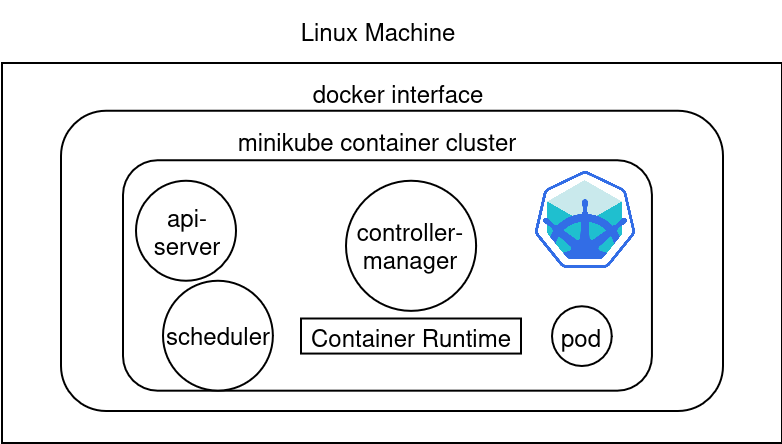
\includegraphics[width=0.9\textwidth]{Design/minikube_driver.png}
\end{figure}

Each component specified in the state of the art for kubernetes will be deployed into this cluster via minikube. This design ensures seamless deployment, developer friendly and extensible scalable design.


\subsection{Network Exposure Design in Kubernetes}
The ingestion of UDP traffic into Kubernetes was approached with the intent to provide a service load balancer and an IP address. This would allow us to create an endpoint for our application, enabling Kubernetes to proxy to the microservices with the help of the built application. Previous chapters discussed exposing UDP traffic as the first challenge to overcome for the realization of our final goal. In this section, the design inspiration stemmed from observing the large adoption of cloud networks and how they exposed Kubernetes services to the outside world. It became evident that there was a need for an external load balancer, which would assign an IP to our service load balancer. The Kubernetes solutions for exposing services in a local setup, as discussed in the state of the art, were limited. Hence, a solution utilizing MetalLB was proposed. MetalLB is a bare-metal load balancer for Kubernetes that allowed us to provide an entry point to our application. The following architecture shows how MetalLB was leveraged



\begin{figure}[H]
\caption{Design of Metal-lb}
\centering
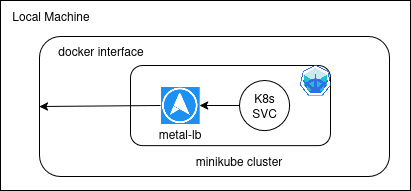
\includegraphics[width=0.8\textwidth]{Design/metal.png}
\end{figure}

From the figure, we can see that MetalLB is intended to be the frontend of our Kubernetes Cluster, ingesting data. It's important to note that MetalLB acts as a Layer 4 network load balancer, which allows it to proxy raw UDP packets into our cluster. This solves the problem of ingestion. The traffic will travel to and from the service, to MetalLB, and then to the outside cluster, and vice versa.



\subsubsection{Sequence Flow for metallb}
\begin{figure}[H]
\caption{Sequence flow for metal-lb}
\centering
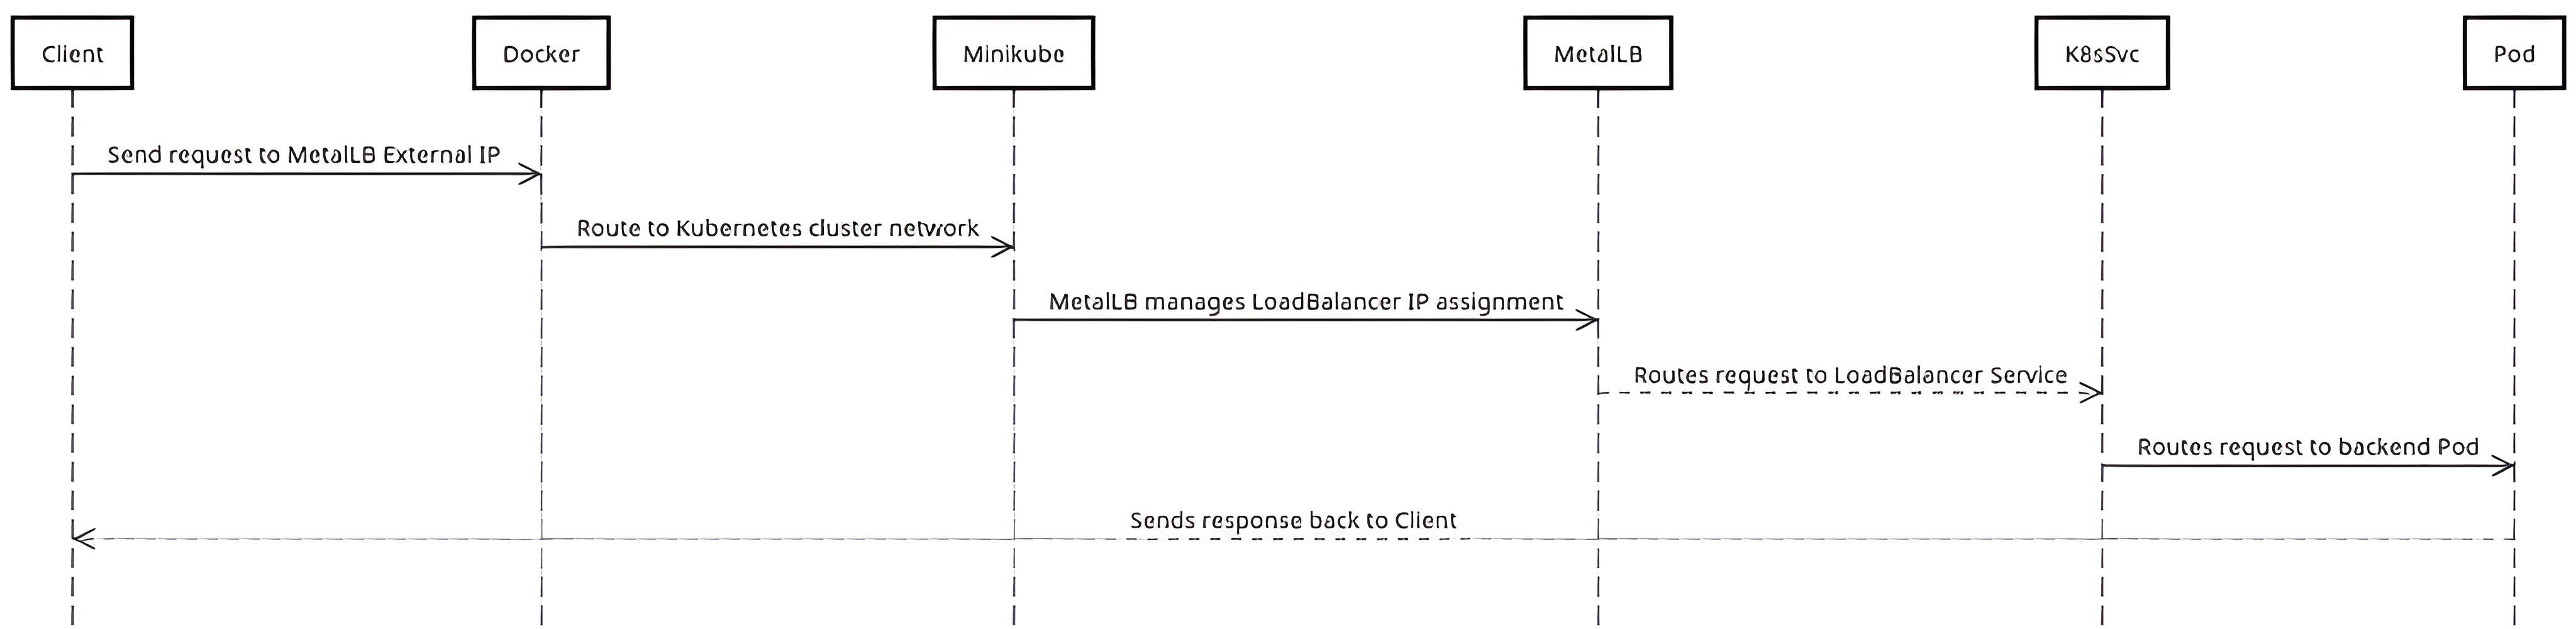
\includegraphics[width=1\textwidth]{Design/metal_sequence.png}
\end{figure}

The client sends a request to the MetalLB IP address. The request is then forwarded through the Docker interface, as MetalLB is deployed on the Minikube cluster, which is running in a Docker container. MetalLB receives the IP address and proceeds to forward the request to the Kubernetes service. This design successfully exposes the Kubernetes service to the outside cluster and allows for the forwarding of raw TCP and UDP packets to our applications.

\section{Design of the Routing and Processing System}

This section presents the design of the routing and processing system for a WebTransport stream-aware routing platform. Design focuses on optimization in configuration, connection managements, packets processing, use of metrics, integration of various microservices and flexibility in command line to facilitate a scalable and resilient streaming design.

\subsection{Configuration-Driven Routing Architecture}



The system adopts a configuration-driven routing approach that allows for dynamic changes and streamlined service management. A central `ServiceConfig` structure defines essential parameters—such as host, port, and endpoint—for each microservice (e.g., audio, video, chat). These configurations are written in a YAML file that is loaded during runtime using a dedicated `ConfigManager` component in Kubernetes. This component enables hot-reloading, so the routing logic can be changed without restarting services. The routing system can therefore be extremely flexible and extensible and easily reconfigured to accommodate emerging needs or varying deployment environments during operation of the system.

The architecture is intended to operate in Kubernetes and utilizes Kubernetes constructs such as ConfigMaps and Secrets to pass routing definitions and TLS credentials to the downstream code.As far as it is concerned, the Router Config is a central configuration file that encapsulates the rules of service routing and protocol behaviors. The router serves as a fast proxy, reading the configuration from this file and redirecting client search requests to the correct backend microservices. This decoupled and declarative model leads to routing behavior that is fully controlled entirely outside of the application's code. This approach aligns with CI/CD principles. The system supports dynamic scaling, safe updates, and operational agility, thereby enabling the router to be deployed in modern cloud-native operations that demand responsiveness and maintainability.


\begin{figure}[h]
\centering
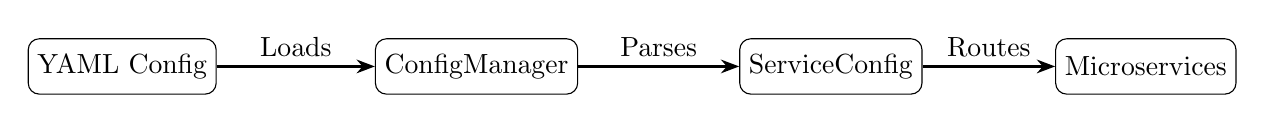
\begin{tikzpicture}[
    box/.style={rectangle, draw, rounded corners, minimum height=2em, minimum width=6em, align=center},
    arrow/.style={-Stealth, thick}
]
    % Nodes
    \node[box] (yaml) at (0,0) {YAML Config};
    \node[box] (manager) at (4.5,0) {ConfigManager};
    \node[box] (service) at (9,0) {ServiceConfig};
    \node[box] (micro) at (13,0) {Microservices};

    % Arrows
    \draw[arrow] (yaml) -- (manager) node[midway, above] {Loads};
    \draw[arrow] (manager) -- (service) node[midway, above] {Parses};
    \draw[arrow] (service) -- (micro) node[midway, above] {Routes};
\end{tikzpicture}
\caption{Configuration-Driven Routing Flow}
\label{fig:config_routing}
\end{figure}

The figure illustrates the flow from a YAML configuration file to the \texttt{ConfigManager}, which parses and stores settings in \texttt{ServiceConfig} structures, enabling routing to microservices. Arrows indicate the sequential process of loading, parsing, and routing configuration data.

\subsection{WebTransport Protocol Handling}

The WebTransport protocol handling system manages QUIC/HTTP3 connections and streams, ensuring reliable communication for real-time streaming. A \texttt{WebTransportRouter} component handles protocol negotiation, stream creation, and HTTP/3 request processing, maintaining connection state. Each QUIC stream is assigned a dedicated buffer to manage packet reassembly and analysis, ensuring efficient handling of incoming data. This design supports high-throughput streaming while maintaining low latency and robust connection management.

\begin{figure}[h]
\centering
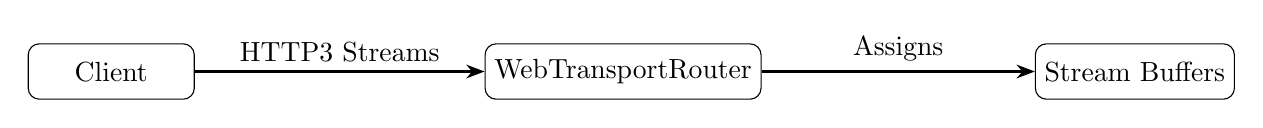
\begin{tikzpicture}[
    box/.style={rectangle, draw, rounded corners, minimum height=2em, minimum width=6em, align=center},
    arrow/.style={-Stealth, thick}
]
    % Nodes
    \node[box] (client) at (0,0) {Client};
    \node[box] (router) at (6.5,0) {WebTransportRouter};
    \node[box] (stream) at (13,0) {Stream Buffers};

    % Arrows
    \draw[arrow] (client) -- (router) node[midway, above] {HTTP3 Streams};
    \draw[arrow] (router) -- (stream) node[midway, above] {Assigns};
\end{tikzpicture}
\caption{WebTransport Protocol Handling}
\label{fig:webtransport}
\end{figure}

The figure depicts a client sending data via QUIC/HTTP3 to the \texttt{WebTransportRouter}, which assigns streams to dedicated buffers for processing. Arrows show the flow of data from the client to the router and then to stream buffers.

\subsection{Packet Parsing and Routing}

The packet parsing and routing system is designed to efficiently process incoming packets by extracting headers and forwarding payloads to the correct microservices. A fixed 32-byte header enables fast and reliable parsing, containing fields like \texttt{track\_id}, \texttt{payload\_len}, and \texttt{track\_type}. The payload is extracted based on the \texttt{payload\_len} field and routed to the appropriate microservice using the \texttt{track\_type} and configuration data. This design ensures low-latency processing and accurate routing in a multiplexed streaming environment.

\begin{figure}[h]
\centering
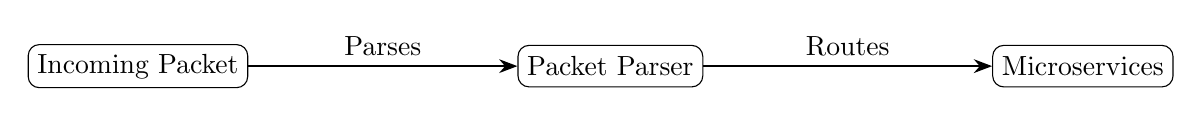
\begin{tikzpicture}[
    box/.style={rectangle, draw, rounded corners, minimum height=1.5em, minimum width=4em, align=center},
    arrow/.style={-Stealth, thick}
]
    % Nodes using absolute positioning
    \node[box] (packet) at (0,0) {Incoming Packet};
    \node[box] (parser) at (6,0) {Packet Parser};
    \node[box] (micro) at (12,0) {Microservices};

    % Arrows
    \draw[arrow] (packet) -- (parser) node[midway, above] {Parses};
    \draw[arrow] (parser) -- (micro) node[midway, above] {Routes};
\end{tikzpicture}
\caption{Packet Parsing and Routing}
\label{fig:packet_parsing}
\end{figure}

The figure shows an incoming packet being processed by the packet parser, which extracts the header and routes the payload to microservices. Arrows indicate the parsing and routing steps.


\subsection{Metrics Logging}
The structure of metrics logging is clearly elaborated in the evaluation (chapter 6). This part contains the overview of the design 


\begin{figure}[h]
\centering
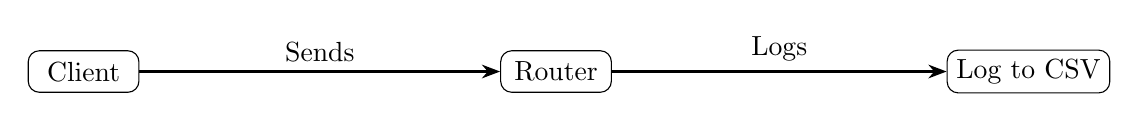
\begin{tikzpicture}[
    box/.style={rectangle, draw, rounded corners, minimum height=1.5em, minimum width=4em, align=center},
    arrow/.style={-Stealth, thick}
]
    % Nodes
    \node[box] (client) at (0,0) {Client};
    \node[box] (router) at (6,0) {Router};
    \node[box] (logger) at (12,0) {Log to CSV};

    % Arrows
    \draw[arrow] (client) -- (router) node[midway, above] {Sends};
    \draw[arrow] (router) -- (logger) node[midway, above] {Logs};
\end{tikzpicture}
\caption{Client Request Routing and Logging}
\label{fig:client_logging}
\end{figure}


The figure illustrates the system collecting metrics via the \texttt{MetricsLogger}, which logs data to CSV and log files. Arrows represent the flow of metric collection and logging.

\subsection{Microservice Proxying}

The microservice proxying system forwards packets to the appropriate microservices with robust error handling and retry mechanisms. It supports flexible data formats, including binary and JSON, to accommodate different service requirements. Custom headers can be added to packets for extensibility and debugging, enabling traceability and future enhancements. This design ensures reliable communication between the router and microservices, supporting a modular and scalable architecture.



\begin{figure}[h]
\centering
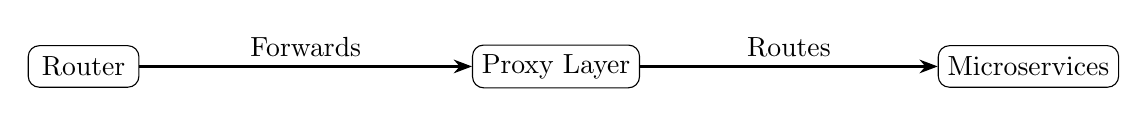
\begin{tikzpicture}[
    box/.style={rectangle, draw, rounded corners, minimum height=1.5em, minimum width=4em, align=center},
    arrow/.style={-Stealth, thick}
]
    \node[box] (router) at (0,0) {Router};
    \node[box] (proxy) at (6,0) {Proxy Layer};
    \node[box] (micro) at (12,0) {Microservices};

    \draw[arrow] (router) -- (proxy) node[midway, above] {Forwards};
    \draw[arrow] (proxy) -- (micro) node[midway, above] {Routes};
\end{tikzpicture}
\caption{Microservice Proxying}
\label{fig:proxying}
\end{figure}

The figure shows the router forwarding packets to a proxy layer, which routes them to microservices with error handling. Arrows depict the forwarding and routing process.



\section{Pulsar Integration Design}

After processing packets such as chat messages, audio streams, or video data, each microservice can optionally publish the output to an Apache Pulsar topic. This mechanism decouples real-time data processing from downstream distribution analytics, storage, or machine learning. The messages of each particular service are sent to a specifically-named topic (e.g., chat-topic, video-topic), which guarantees a separation of concerns as well as scalability.

This design enables easy integration with real-time data consumers, allows for per-service configuration of Pulsar usage and allows for flexibility in order to enable/disable publishing dynamically.



\begin{figure}[h]
\centering
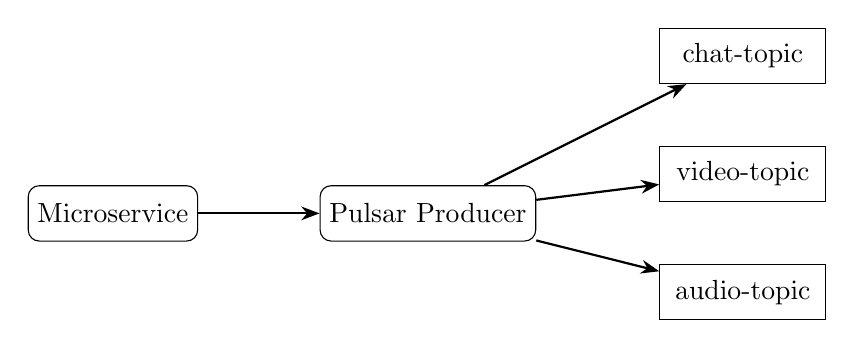
\begin{tikzpicture}[
    box/.style={rectangle, draw, rounded corners, minimum height=2em, minimum width=6em, align=center},
    arrow/.style={-Stealth, thick},
    topic/.style={rectangle, draw, minimum height=2em, minimum width=6em, align=center}
]

% Nodes
\node[box] (micro) at (0,0) {Microservice};
\node[box] (producer) at (4,0) {Pulsar Producer};

% Topic nodes
\node[topic] (chat) at (8,2) {chat-topic};
\node[topic] (video) at (8,0.5) {video-topic};
\node[topic] (audio) at (8,-1) {audio-topic};

% Arrows
\draw[arrow] (micro) -- (producer);
\draw[arrow] (producer) -- (chat);
\draw[arrow] (producer) -- (video);
\draw[arrow] (producer) -- (audio);

\end{tikzpicture}
\caption{Microservice to Pulsar Topics Integration}
\label{fig:microservice_pulsar}
\end{figure}



\section{Complete System Architecture}

The following architecture is a high-level technical architecture diagram which entails the complete proposed solution. The sections above delved deep into each components individually and this is the final high-level overview of our dissertation

\begin{figure}[H]
\caption{System Architecture}
\centering
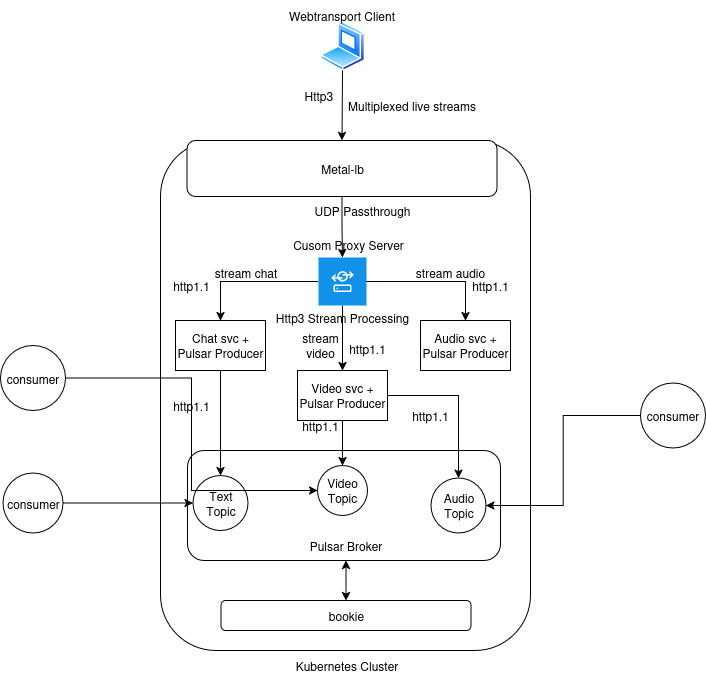
\includegraphics[width=1\textwidth]{Design/Design_Solution.png}
\end{figure}

The proposed architecture system is a real-time streaming system based on a modular structure built to support scaling, low latency communication, and efficient data processing and distribution within a cloud-native infrastructure. It starts with ingest layer where client sends streams of data with a webtransport client connects through HTTP/3 a QUIC-based protocol allowing to establish a single transport connection but with multiplexing multiple data streams in the connection video, audio, and chat. The load balancer in the Kubernetes cluster is MetalLB, which is exclusively enabled to provide UDP passthrough for the minikube ckuster to facilitate the forwarding of QUIC connection (entire UDP packets) to the internal components. The system is centered around a custom proxy server that will terminate the HTTP/3 connection, demultiplexes the stream it receives, and forwards each individual data stream to the appropriate microservice over HTTP/1.1. This server effectively acts as both a protocol gateway and a routing mechanism.

The application layer is based on different microservices of chat, video, and audio developed which is responsible for handling its own set of data and are independent from each other. These microservices publishes the data to Apache Pulsar after processing, acting as a producer in the event streaming system. The Pulsar cluster will have a broker handling the routing and dispatching of messages, different topics that logically segregate each type of data (Text Topic, Video Topic, Audio Topic) and it will have a persistent storage backend consisting of the Bookie pods of Apache BookKeeper so that persistant data storage and recovery from faults are possible. Finally, on the consumption level, independent consumer applications subscribes to the Pulsar topics and receive data asynchronously. This decouples the data ingestion and downstream processing, allowing to enable use cases of real-time streaming, analytics or storage with modularity and scalability in the system.
\label{sec:OverviewOfDesign}

\section {Summary}
The proposed system is a real-time streaming architecture that is modular and scalable, designed to support low-latency multimedia communication using WebTransport, Kubernetes, and Apache Pulsar. The architecture breaks the problem space into smaller modules which are developed independently and then combined to form a whole solution. On the client side, WebTransport is used to send data, and WebTransport runs on QUIC to enable data multiplexing across different data streams in a single connection i.e. audio, video and chat. The design will prevent Head-of-Line blocking. A typical packet transmitted has a 32-byte header composed of track\_id, payload\_len and track\_type fields and a variable length payload. The format is capable of extending; it is useful in routing for diversity of data types.

Inside the Kubernetes cluster, a single-node Minikube setup is used for simplicity, leveraging the Docker driver to eliminate virtual machine overhead and enable shared networking. MetalLB is used as a bare metal load balancer that exposes QUIC-based UDP traffic to components of the kubernetes cluster, enabling the external WebTransport clients to connect to internal services. Its routing logic is config-driven, user-managed through YAML-based ConfigMaps and allows for dynamic updates and reloading of routing configurations without system restarts. The core of this solution is the WebTransportRouter, a custom component that accepts and deals with QUIC/HTTP3 streams by attaching each track with its own explicitly associated buffer of streams. This guarantees that audio, video and chat information is manipulated in a low latency basis for redirections. Once the component performs initial parsing, it sends each stream to its respective microservice through HTTP/1.1 via a proxy server that acts as a reliable gateway between the transport and application layers.

At the application layer, separate stateless microservices are responsible for processing specific types of data such as audio, video, or chat. Each microservice publishes the processed data to its corresponding Apache Pulsar topic—for instance, chat-topic or video-topic—thereby enabling a decoupled and scalable processing model. Apache Pulsar is used as the main system for handling event streams. It consists of a broker which receives data for a specific topic and it stored multiple topic's logical association, with each topic keeping different types of data separate (like audio, video, or chat). To ensure data is safely stored and can be recovered if something goes wrong, Apache BookKeeper is used in the background through components called Bookie. On the receiving side, different consumer applications connect to Pulsar and subscribe to specific topics to get the data they need. By keeping the parts that send, process, and receive data separate, the system stays flexible, reliable, and easy to scale for real-time streaming or analytics tasks.


% \section{Detail 1 of the Design}
% \subsection{Aspect \#1}

% \subsubsection{Detail of Aspect  \#1}

% \subsubsection{Another Detail of Aspect  \#1}


% \subsection{Aspect \#2}

% \subsubsection{Detail of Aspect  \#2}

% \subsubsection{Another Detail of Aspect  \#2}


% \section{Detail 2 of the Design}

% \section{Summary}
% \label{sec:SummaryDesign}

% Every chapter aside from the first and last chapter should conclude with a summary. 
\chapter{Implementation}

\section{Introduction}
The implementation chapter translates the proposed WebTransport/QUIC streaming architecture in Chapter 4 into a fully working, reproducible system. It begins by preparing the local development environment by installing Minikube \cite{minikube-docs} with its Docker driver on Linux Mint, enabling MetalLB \cite{metallb-docs} for external Load-Balancer Internet Protocol (IP) addresses, and configuring Wireshark \cite{wireshark-docs} together with self-signed Transport Layer Security (TLS) certificates so that encrypted QUIC traffic can be captured and inspected. A Domain Name System (DNS) entry in /etc/hosts binds the synthetic domain quic-aioquic.com to the cluster’s MetalLB range, ensuring that both browser clients and backend services resolve the same address. With the groundwork in place, the chapter progresses through three tightly coupled tiers: (1) a browser-based WebTransport client that captures video, audio, chat, file and screen-share data, packetises each stream, and transmits them over independent unidirectional QUIC streams; (2) a Python router built on aioquic \cite{aioquic-repo} that receives these streams, parses the custom 32-byte packet header, and routes payloads to backend microservices via hot-reloadable Yet Another Markup Language (YAML) rules; and (3) a set of generic, YAML-configured microservices that expose HyperText Transfer Protocol (HTTP) endpoints, optionally forward data to Apache Pulsar, and run inside Minikube as scalable Deployments. Finally, the entire stack (router, microservices, and Pulsar) is containerised and deployed through Kubernetes manifests that include Secrets for certificates, ConfigMaps for live configuration, and LoadBalancer Services for external reachability, leveraging Apache Pulsar \cite{pulsar-helm-repo} for message streaming.


% Describing Minikube installation process
\section{Installation of Minikube}
The host operating system of the machine at work is Linux Mint, a Debian-based operating system. The steps below outline the installation steps, ensuring a working setup for running a local Kubernetes cluster.

% Providing installation commands
To install Minikube the following commands are executed in the terminal:

\begin{lstlisting}[breaklines=true,basicstyle=\small\ttfamily,frame=single]
curl -LO https://github.com/kubernetes/minikube/releases/latest/download/minikube-linux-amd64
sudo install minikube-linux-amd64 /usr/local/bin/minikube && rm minikube-linux-amd64
\end{lstlisting}

After running these commands Minikube is up and running successfully. To make sure that the installation is working, run Minikube by typing the following:

\begin{lstlisting}[breaklines=true,basicstyle=\small\ttfamily,frame=single]
minikube start
\end{lstlisting}

% Explaining Minikube's default behavior
Note that the \texttt{minikube start} command uses the Docker driver by default. Minikube runs within a Docker container, which provides logical separation from the host system. This containerized approach ensures efficient resource utilization and isolation from the host environment.

% Including figure for CPU and memory usage
\begin{figure}[h!]
    \centering
    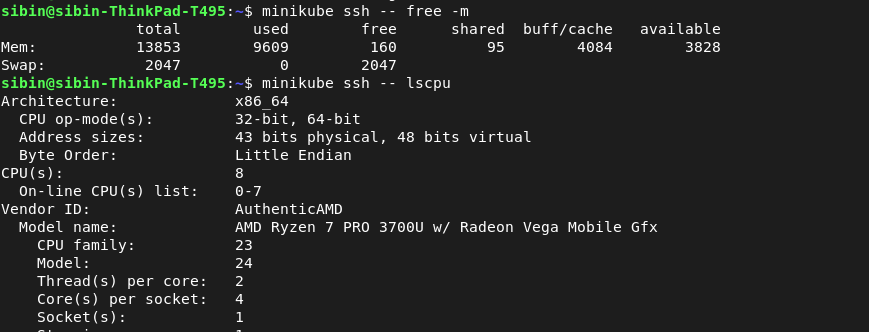
\includegraphics[width=0.8\textwidth]{implementation/minikube-cpunmem.png}
    \caption{Minikube CPU and Memory Usage}
    \label{fig:minikube-cpu-and-memory}
\end{figure}

Since Minikube operates within a container, it leverages the host operating system's kernel and configuration by default. This setup allows the Kubernetes cluster to access additional resources from the host, optimizing performance and scalability for local development and testing.

% Describing kubectl installation
It is important to note that \texttt{kubectl}, the Kubernetes command-line tool, is automatically installed alongside Minikube. To confirm the pods are running in the cluster, run the following command:

\begin{lstlisting}[breaklines=true,basicstyle=\small\ttfamily,frame=single]
kubectl get pods
\end{lstlisting}

% Including figure for kubectl presence
\begin{figure}[h!]
    \centering
    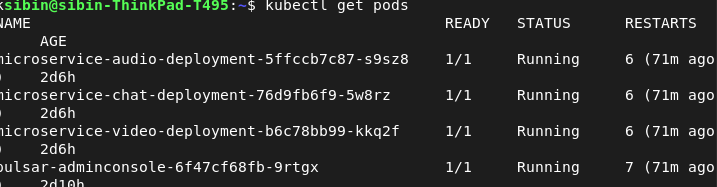
\includegraphics[width=0.8\textwidth]{implementation/pods.png}
    \caption{Verification of Kubectl Presence}
    \label{fig:kgetpods}
\end{figure}

% Confirming successful installation
The Minikube cluster and Kubernetes have been successfully installed and configured on the system. This setup provides a fully working local Kubernetes setup which is ready for deploying and managing applications.

% \section{Installation of Minikube}
% Firstly the host os of the machine at work is Linux Mint which is debian based operating system. An installation for this specific platform is needed. 


% curl -LO https://github.com/kubernetes/minikube/releases/latest/download/minikube-linux-amd64
% sudo install minikube-linux-amd64 /usr/local/bin/minikube && rm minikube-linux-amd64
% Now minikube is successfully installed and working which is verified by

% minikube start

% Note that minikube start starts to run with docker interface by default. It runs on a docker container providing logical seperation.

% \begin{figure}[h!]
% \centering
% 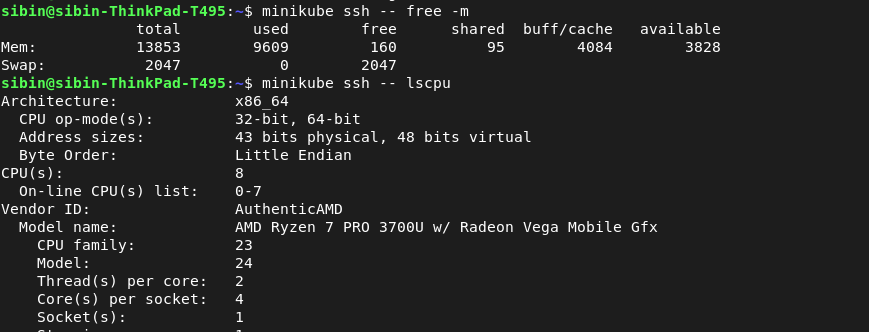
\includegraphics[width=0.8\textwidth]{implementation/minikube-cpunmem.png}
% \caption{Minikube CPU and Memory}
% \label{fig:minikube-cpu-and-memory}
% \end{figure}
% Note that since we run it in a container, it uses host operating system's operating system and configuration by default. This allows us to use more resources for our kubernetes cluster.

% It is to note that kubectl is installed by default when minikube is installed. We can check the existance of pods by running kubectl get pods

% \begin{figure}[h!]
% \centering
% 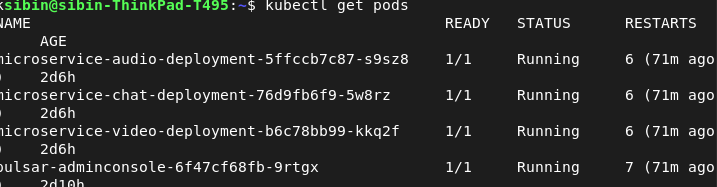
\includegraphics[width=0.8\textwidth]{implementation/pods.png}
% \caption{Kubectl Presence}
% \label{fig:kgetpods}
% \end{figure}

% The minikube cluster and kubernetes have been successfully installed in the system.

% \section{Configuration Metal-lb}
% Metal-lb is a loadbalancer which operates at Layer 4 which is required for exposing all services of type load balancer in our kubernetes cluster. Minikube provides with easy installation with addons options

% minikube addons list
% It lists several addons provided by minikube. In it it can be seen that metallb is disabled which needs to be enabled so to enable it run the following command

% minikube addons enable metal-lb

% Now the metallb requires a range of ip addresses so it can assign to services created within kubernetes

% When minikube container was started with minikube start, it created a network interface in background for minikube ie kubernetes environment which can be verifed with 
% ifconfig. For machine at use, it the interface was name was br-5d.. and had values  inet 192.168.49.1  netmask 255.255.255.0  broadcast 192.168.49.255. This essentially meant the last octet is open from 0-255, which creates a subnet and can be represented by
% 192.168.49.0/24. 
% minikube addons configure metallb
% Enter Load Balancer Start IP: 192.168.49.1
% Enter Load Balancer End IP: 192.168.49.250
% This configures load balancer for these ip address ranges




% Describing MetalLB configuration process
\section{Configuration of MetalLB}
MetalLB is a load balancer that operates at Layer 4, which is essential for exposing all services of type LoadBalancer in our Kubernetes cluster. Minikube provides a straightforward installation process for MetalLB through its addons feature.

% Listing available addons
To see the existing addons in Minikube, run the following command:

\begin{lstlisting}[breaklines=true,basicstyle=\small\ttfamily,frame=single]
minikube addons list
\end{lstlisting}

This command lists several addons provided by Minikube. Among them, you will notice that MetalLB is disabled by default. To enable it, the following command is executed:

\begin{lstlisting}[breaklines=true,basicstyle=\small\ttfamily,frame=single]
minikube addons enable metallb
\end{lstlisting}

% Explaining IP range configuration for MetalLB
MetalLB requires a range of IP addresses to assign to services created within the Kubernetes cluster. When the Minikube container was started with the \texttt{minikube start} command, it created a network interface in the background for the Minikube (i.e., Kubernetes) environment. This can be verified by running:

\begin{lstlisting}[breaklines=true,basicstyle=\small\ttfamily,frame=single]
ifconfig
\end{lstlisting}

For the machine in use, the network interface was named \texttt{br-5d..} and had the following values: \texttt{inet 192.168.49.1}, \texttt{netmask 255.255.255.0}, \texttt{broadcast 192.168.49.255}. This indicates that the last octet is open from 0 to 255 which creates a subnet that can be represented by \texttt{192.168.49.0/24}.

% Configuring MetalLB IP range
To configure MetalLB with appropriate IP address ranges, run the following command:

\begin{lstlisting}[breaklines=true,basicstyle=\small\ttfamily,frame=single]
minikube addons configure metallb
\end{lstlisting}

During configuration, it would prompt asking to enter the start and end IP addresses for the load balancer:

\begin{lstlisting}[breaklines=true,basicstyle=\small\ttfamily,frame=single]
Enter Load Balancer Start IP: 192.168.49.1
Enter Load Balancer End IP: 192.168.49.250
\end{lstlisting}

This configures the MetalLB load balancer to expose applications within the specified IP address range, enabling it to assign IPs to LoadBalancer-type services in the Kubernetes cluster.

% \section{Wireshark}
% To install wireshark and successfully capture traffic, the following process was followed.
% sudo apt install wireshark
% wireshark 
% this opens out wireshark
% It asks you to monitor a specific network interface which when selected started capturing realtime traffic to and from the network interface. Here its to note that higher level application protocols which are encrypted can be captured but not looked into due to their encryption with standard tls protocol. We need tls session keys which would help us decrypt the communication. The session keys can either be logged from the client and server and can be loaded from
% edit->preferences->protcols->tls->premaster secret log name->load the tls session keys

% This process helps to decrypt the TLS encrypted data captured over the network.


% Describing Wireshark installation and usage process
\section{Network Traffic Capture}
To install Wireshark and successfully capture network traffic on Linux Mint OS, the following process was followed.

% Providing installation commands
\subsection{Run Commands}
First, install Wireshark using the package manager by executing the following command:

\begin{lstlisting}[breaklines=true,basicstyle=\small\ttfamily,frame=single]
sudo apt install wireshark
\end{lstlisting}

Launch Wireshark by running:

\begin{lstlisting}[breaklines=true,basicstyle=\small\ttfamily,frame=single]
wireshark
\end{lstlisting}

Above command opens up the Wireshark application. Upon launching, Wireshark prompts you to select a specific network interface to monitor. Once an interface is selected, Wireshark begins capturing real-time traffic to and from the chosen network interface.



% Describing Chromium TLS key logging process
\subsection{Logging Chromium Client TLS Keys}
To log the TLS session keys for the Chromium client, the following steps were performed to ensure proper configuration and logging of the keys for use in decrypting network traffic.

% Providing commands for logging TLS keys
First, terminate any running instances of Chromium by executing the following command:

\begin{lstlisting}[breaklines=true,basicstyle=\small\ttfamily,frame=single]
pkill chromium
\end{lstlisting}

Next, set the environment variable to specify the path for the TLS key log file:

\begin{lstlisting}[breaklines=true,basicstyle=\small\ttfamily,frame=single]
export SSLKEYLOGFILE=$HOME/premaster-secret/sslkeylogfile.log
\end{lstlisting}

Then, restart Chromium to begin logging the TLS keys to the specified path.

% Including figure for SSL key log
\begin{figure}[h!]
    \centering
    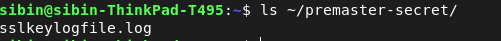
\includegraphics[width=0.8\textwidth]{implementation/sslkeylog.png}
    \caption{Chromium Client's SSL Key Log}
    \label{fig:chromiumssl}
\end{figure}

\subsection{Configuring TLS Keys in Wireshark}

This process successfully logs the TLS session keys to the designated file, enabling the decryption of TLS-encrypted traffic captured from the Chromium client.

% Explaining limitations and TLS decryption
It is important to note that higher-level application protocols, which are encrypted using the standard TLS protocol, can be captured but cannot be inspected directly due to their encryption. To decrypt such communications, TLS session keys are required. These session keys can be logged from the client or server and loaded into Wireshark for decryption.

% Configuring Wireshark for TLS decryption
To decrypt TLS traffic, TLS session keys must be loaded and to load the keys, following steps in Wireshark were followed:

\begin{enumerate}
    \item Go to \texttt{Edit -> Preferences -> Protocols -> TLS}.
    \item In the TLS settings, locate the \texttt{Pre-Master Secret Log Filename} field.
    \item Load the TLS session keys by adding the path of the log file which contain the keys.
\end{enumerate}

This process enables Wireshark to decrypt the TLS-encrypted data captured over the network, allowing for detailed inspection of the communication.



% \subsection{Logging Chromium Client TLS keys}
% killing running instance of chromium -> pkill chromium
% export SSLKEYLOGFILE=$HOME/premaster-secret/sslkeylogfile.log
% and starting the chromium again
% This logs the keys to the specified path
% \begin{figure}[h!]
% \centering
% 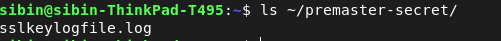
\includegraphics[width=0.8\textwidth]{implementation/sslkeylog.png}
% \caption{Chromium Client's SSLKEYLOG}
% \label{fig:chromiumssl}
% \end{figure}


% \section{Certificate Management Process}
% The first step to working with the state of the art Webtransport Streams Http3 Router, it was identified that a need for certificate is substantial as without which the data could not be sent over the specified protocol. Since it was not feasible to own a domain as approach to creating a self signed certificate was taken.

% The following commands created a self signed certificate for a new domain

% openssl req -x509 -newkey rsa:4096 -keyout tls.key -out tls.crt -days 365 -nodes -subj "/CN=quic-aioquic.com:

% This requests openssl for a rsa keypair and creates cert and key with an expiry of 365 days with the Subject alternative name and CName set to the custo domain quic-aioquic.com
% Now in order to use the certificate the client must forward request to the particular domain and the client must itself trust the domain. In order to do that and snce we were working with browser client chrome. Through settings we could upload the certificate

% Settings -> Privary and Security -> Manage Certificates -> Installed Certificates by You -> Import

% This way the client can be trusted





% Describing certificate management process
\section{Certificate Management}
To enable secure communication with the state-of-the-art WebTransport Streams HTTP/3 Router, it was determined that a certificate is essential, as data transmission over the specified protocol requires encryption. Since acquiring a domain was not feasible, the approach of creating a self-signed certificate was adopted.

% Providing commands for creating a self-signed certificate
The following command was used to generate a self-signed certificate for a custom domain:

\begin{lstlisting}[breaklines=true,basicstyle=\small\ttfamily,frame=single]
openssl req -x509 -newkey rsa:4096 -keyout tls.key -out tls.crt -days 365 -nodes -subj "/CN=quic-aioquic.com"
\end{lstlisting}

This command instructs OpenSSL to create an RSA key pair, generating both a certificate (\texttt{tls.crt}) and a private key (\texttt{tls.key}) with an expiration period of 365 days. The \texttt{-nodes} flag ensures the private key is not encrypted, and the Subject Alternative Name and Common Name (CN) are set to the custom domain \texttt{quic-aioquic.com}.

% Explaining certificate usage and client configuration
To utilize the certificate, the client must forward requests to the specified domain, and the client itself must trust the domain. Since the client in use was the Chrome browser, the self-signed certificate was imported through the browser's settings to establish trust.

% Providing steps for importing the certificate in Chrome
The certificate can be imported by following these steps in Chrome:

\begin{enumerate}
    \item Navigate to \texttt{Settings -> Privacy and Security -> Manage Certificates}.
    \item Under the \texttt{Installed Certificates by You} section, select \texttt{Import}.
    \item Follow the prompts to upload the \texttt{tls.crt} certificate file.
\end{enumerate}

This process ensures that the Chrome client trusts the self-signed certificate, enabling secure communication with the WebTransport Streams HTTP/3 Router.


% \section{DNS entry}
% In order to work with a DNS entry for your local setup we need a domain name resolution process to be in place. Now that the certificates are structed, requests are explictly checked for the domain. For the linux machine, the configuration changes was done to /etc/hosts directory where an entry for dns was inputted. for my system I added this line

% 192.168.49.201 quic-aioquic.com
% It maps the domain name to the specific ip address


% Describing DNS entry configuration process
\section{DNS Entry Configuration}
To enable domain name resolution for the local setup, a DNS entry must be configured. With the certificates properly structured, requests are explicitly checked for the specified domain. On a Linux machine, this configuration is achieved by modifying the \texttt{/etc/hosts} file to include a DNS entry that maps the domain to a specific IP address.

% Providing the DNS entry configuration
For the system in use, the following line was added to the \texttt{/etc/hosts} file:

\begin{lstlisting}[breaklines=true,basicstyle=\small\ttfamily,frame=single]
192.168.49.201 quic-aioquic.com
\end{lstlisting}

This entry maps the domain name \texttt{quic-aioquic.com} to the IP address \texttt{192.168.49.201}, ensuring proper domain name resolution for the local setup.




% Describing the client construction process
\section{Client Construction}
The construction of the client was accomplished using several core components, each designed to ensure a robust and user-friendly streaming experience. These components are detailed below.

% Describing the user interface design
\subsection{User Interface Design}
The client's user interface is created for clarity and functionality, offering an intuitive overview of the streaming process. The layout is structured using a responsive \textbf{CSS Grid} (\texttt{.container}), which divides the main content into distinct panels for streamlined user interaction.

\begin{itemize}
    \item \textbf{Video \& Audio Stream Panel} (\texttt{.panel}): This panel prominently displays the local video feed (\texttt{<video id="localVideo">}) and includes controls for initiating or stopping streaming, toggling video quality, and starting or stopping optional file and screen data streams.
    \item \textbf{Live Chat Panel} (\texttt{.panel}): This features a scrollable message display area (\texttt{.chat-\allowbreak{}messages}) and an input field with a send button (\texttt{.chat-input}) for real-time text communication.
    \item \textbf{Metrics Display} (\texttt{.metrics}): This provides at-a-glance performance indicators, including the count of video frames, audio packets, chat messages sent, and the calculated data transfer rate.
    \item \textbf{Status Bar} (\texttt{\#status}): This offers immediate feedback on the WebTransport connection state.
    \item \textbf{System Logs Panel} (\texttt{.logs}): This acts as a console, displaying critical information about stream creation, packet transmission, and error events, which is essential for monitoring and debugging during development and testing.
\end{itemize}

The visual design adopts a dark theme using CSS, enhancing readability in low-light conditions and providing a modern aesthetic. Buttons are styled with distinct colors (\texttt{.btn-start}, \texttt{.btn-stop}, \texttt{.btn-toggle}) to clearly indicate their actions and current states, such as \texttt{disabled} styling.

% Describing WebTransport connection setup
\subsection{WebTransport Connection Setup}
Establishing a reliable connection to the WebTransport server is the foundational step for all streaming operations. This is managed within the \texttt{WebTransportStreamer} class's \texttt{startStreaming()} method. The connection is initiated by creating a new \texttt{WebTransport} instance, specifying the server URL (\texttt{https://quic-aioquic.com:4433/wt}), which points to the secure QUIC endpoint of the server.

\begin{lstlisting}[breaklines=true,basicstyle=\small\ttfamily,frame=single]
//Initialize WebTransport connection to the server endpoint
this.transport = new WebTransport(this.serverUrl);
\end{lstlisting}

To ensure robust operation, event listeners are set up for \textbf{connection state changes} (\texttt{this.transport.onstatechange}) and \textbf{errors} (\texttt{this.transport.onerror}). These listeners are critical for monitoring the connection's health:

\begin{itemize}
    \item \texttt{onstatechange}: Updates the UI status and triggers \texttt{stopStreaming()} if the connection \texttt{state} transitions to \texttt{'closed'}, indicating a graceful shutdown or an unexpected termination.
    \item \texttt{onerror}: Catches any underlying transport errors, logs them to the console, and initiates \texttt{stopStreaming()} to clean up resources.
\end{itemize}

\begin{lstlisting}[breaklines=true,basicstyle=\small\ttfamily,frame=single]
this.transport.onstatechange = () => {
    this.log(`Transport state: ${this.transport.state}`, 'info');
    if (this.transport.state === 'closed') {
        this.stopStreaming();
    }
};
this.transport.onerror = (event) => {
    this.log(`Transport error: ${event.message}`, 'error'); #logs error
    this.stopStreaming();
};
\end{lstlisting}

The \texttt{await this.transport.ready;} promise ensures that the application waits until the WebTransport connection is established before starting with media capture and stream creation which prevents operations on a disconnected transport. This ensures a stable foundation for subsequent streaming activities.

% Describing media capture and stream initialization
\subsection{Media Capture and Stream Initialization}
Once the WebTransport connection is ready, the client proceeds to capture local media and prepare the data streams for transmission.

\subsubsection{Video/Audio Capture}
Media access is prompted using the \textbf{WebRTC \texttt{getUserMedia} API}, this requests the user for permission to access camera and microphone. The \texttt{constraints} object defines the desired media properties:

\begin{itemize}
    \item \texttt{video}: Configured for resolutions \texttt{640x480} at \texttt{15fps} (Standard Quality) or \texttt{1280x720} at \texttt{30fps} (High Quality), with change of the \texttt{isHighQuality} flag.
    \item \texttt{audio}: Includes \texttt{echoCancellation} and \texttt{noiseSuppression} to improve audio clarity.
\end{itemize}

\begin{lstlisting}[breaklines=true,basicstyle=\small\ttfamily,frame=single]
const mediaConstraints = {
    video: {
        //Set video dimensions based on quality mode selection
        width: this.isHighQuality ? 1280 : 640,
        height: this.isHighQuality ? 720 : 480,
        //Configure frame rate for optimal performance
        frameRate: this.isHighQuality ? 30 : 15
    },
    audio: {
        //Apply audio processing enhancements
        echoCancellation: true,
        noiseSuppression: true
    }
};
//Capture user media with specified constraints
this.mediaStream = await navigator.mediaDevices.getUserMedia(mediaConstraints);
//Display captured video in local preview element
this.elements.localVideo.srcObject = this.mediaStream;
\end{lstlisting}

The captured \texttt{mediaStream} is assigned to the \texttt{<video id="localVideo">} element, allowing the user to see their own video feed. A \texttt{Promise} is used to wait for the video element to trigger \texttt{loadeddata}, ensuring the media stream is fully ready before processing.

\subsubsection{Stream Creation}
WebTransport's strength lies in its support for \textbf{multiplexing} via individual streams over a single connection. The client leverages \textbf{unidirectional streams} (\texttt{create\allowbreak{}Bidirectional\allowbreak{}Stream()}) for each distinct data type:

\begin{itemize}
    \item \texttt{this.videoStream}: For outgoing video frames.
    \item \texttt{this.audioStream}: For outgoing audio packets.
    \item \texttt{this.chatStream}: For outgoing chat messages.
    \item \texttt{this.fileStream}: For sending arbitrary file data.
    \item \texttt{this.screenStream}: For sending screen share data.
\end{itemize}

\begin{lstlisting}[breaklines=true,basicstyle=\small\ttfamily,frame=single]
#Initialize separate WebTransport streams for different data types
#Video stream for transmitting video frame data
this.videoStream = await this.transport.createUnidirectionalStream();
#Audio stream for transmitting audio packet data  
this.audioStream = await this.transport.createUnidirectionalStream();
#Chat stream for transmitting text messages
this.chatStream = await this.transport.createUnidirectionalStream();
\end{lstlisting}

With separate unidirectional streams, the client sends different types of data independently without head-of-line blocking, enhancing real-time performance and simplifying server-side processing.

% Describing packet construction and sending
\subsection{Packet Construction and Sending}
A custom packet format is implemented to encapsulate various data types for transmission over WebTransport streams, allowing the server to easily identify and process incoming data.

\subsubsection{Packet Format}
Each packet that is sent over a WebTransport stream follows a predefined format consisting of a \textbf{32-byte header} followed by a variable-length \textbf{payload}. The header provides essential metadata:

\begin{itemize}
    \item \textbf{\texttt{track\_id} (16 bytes)}: A string identifier, such as \texttt{'live\_video'}, \texttt{'test\_audio'}, \texttt{'live\_chat'}, used by the receiver to identify the packet's content within its stream and is padded with null bytes if it's shorter than 16 bytes.
    \item \textbf{\texttt{payload\_length} (4 bytes)}: A 32-bit unsigned integer that indicates the exact size of the payload in bytes which is required for correct payload reading.
    \item \textbf{\texttt{track\_type} (12 bytes)}: A string, such as \texttt{'video'}, \texttt{'audio'}, \texttt{'chat'}, \texttt{'file'}, \texttt{'screen'}, classifying the general type of data, padded to 12 bytes.
\end{itemize}

The \texttt{buildPacket()} function assembles this structure:

\begin{lstlisting}[breaklines=true,basicstyle=\small\ttfamily,frame=single]
buildPacket(trackId, trackType, payload, forceSize = null) {
    let finalPayload = payload;
    if (forceSize && forceSize > payload.length) {
        finalPayload = new Uint8Array(forceSize);
        finalPayload.set(payload, 0);
        for (let i = payload.length; i < forceSize; i++) { #Padding
            finalPayload[i] = i % 256; //Padding pattern
        }
    }

    const header = new ArrayBuffer(32);
    const view = new DataView(header);
    //Set track_id (bytes 0-15)
    new Uint8Array(header, 0, 16).set(this.encoder.encode(trackId.substring(0, 16)));
    //Set payload_length (bytes 16-19)
    view.setUint32(16, finalPayload.length, false); //false for big-endian
    //Set track_type (bytes 20-31)
    new Uint8Array(header, 20, 12).set(this.encoder.encode(trackType.substring(0, 12)));

    const packet = new Uint8Array(header.byteLength + finalPayload.length);
    packet.set(new Uint8Array(header), 0);
    packet.set(finalPayload, header.byteLength);
    this.bytesTransferred += packet.length;
    return packet;
}
\end{lstlisting}

The \texttt{forceSize} parameter allows the client to artificially inflate packet size with padding, serving as a testing feature to analyze the impact of larger packets on network performance and server-side buffer management.

\subsubsection{Sending Logic}
Data is sent using the \texttt{WritableStreamDefaultWriter} associated with each WebTransport stream. The \texttt{loggedWrite()} helper function wraps the \texttt{writer.write()} operation, providing robust error handling and immediate logging feedback:

\begin{lstlisting}[breaklines=true,basicstyle=\small\ttfamily,frame=single]
//Asynchronous function to send packets with comprehensive error handling
async transmitWithLogging(streamWriter, packetData, dataType) {
    try {
        //Attempt to write packet data to the WebTransport stream
        await streamWriter.write(packetData);
        //Log successful transmission with packet details
        this.log(`Successfully transmitted ${dataType} packet: ${packetData.length} bytes`, 'success');
        return true;
    } catch (transmissionError) {
        //Log detailed error information for debugging
        this.log(`Transmission failed for ${dataType} packet: ${transmissionError.message}`, 'error');
        return false;
    }
}
\end{lstlisting>

This function logs every successful packet transmission, including its type and size, aiding in real-time monitoring. In case of failure, such as stream closed, network issue, an error is logged, ensuring communication issues are immediately visible. The \texttt{writer.releaseLock()} is used after sending test packets to allow re-acquisition for continuous streaming.

% Describing video streaming implementation
\subsection{Video Streaming Implementation}
Video streaming is handled by continuously capturing frames from the local video feed, processing them, and sending them over the dedicated video WebTransport stream. The \texttt{startVideoCapture()} method uses a hidden \texttt{HTMLCanvasElement} as an intermediary to process video frames:

\begin{lstlisting}[breaklines=true,basicstyle=\small\ttfamily,frame=single]
const canvas = document.createElement('canvas');
const ctx = canvas.getContext('2d');
canvas.width = this.isHighQuality ? 1280 : 640;
canvas.height = this.isHighQuality ? 720 : 480;
this.videoWriter = this.videoStream.getWriter();
\end{lstlisting}

A \texttt{captureLoop()} function recursively calls itself using \texttt{setTimeout} to maintain a consistent frame rate (15 FPS for standard quality, 30 FPS for high quality). The loop includes:

\begin{enumerate}
    \item \textbf{Frame Capture}: \texttt{ctx.drawImage(this.elements.localVideo, 0, 0, canvas.width\allowbreak{}, canvas.height);} draws the current video frame onto the canvas.
    \item \textbf{Encoding}: \texttt{canvas.toDataURL('image/jpeg', quality);} converts the canvas content into a JPEG image data URL, with \texttt{quality} set to 0.7 for standard or 0.9 for high quality.
    \item \textbf{Binary Conversion}: The Base64-encoded image data is converted into a \texttt{Uint8Array} payload.
    \item \textbf{Packetization and Sending}: The \texttt{buildPacket()} method creates a packet with \texttt{track\_id 'live\_video'} and \texttt{track\_type 'video'}, applying a \texttt{forceSize} of 2500 bytes for high-quality streaming to test network handling. The packet is sent via \texttt{this.loggedWrite(this.videoWriter, packet, 'VIDEO')}.
    \item \textbf{Metrics Update}: \texttt{this.videoFrameCount++} increments the counter for UI display.
\end{enumerate}

This approach provides granular control over video encoding and packet size, facilitating experimental analysis of quality settings and packet sizes.

% Describing audio streaming implementation
\subsection{Audio Streaming Implementation}
Audio streaming leverages the \textbf{Web Audio API} for efficient capture and processing of microphone input. The \texttt{startAudioCapture()} method sets up an audio processing pipeline:

\begin{lstlisting}[breaklines=true,basicstyle=\small\ttfamily,frame=single]
const audioContext = new (window.AudioContext || window.webkitAudioContext)();
await audioContext.resume();
const source = audioContext.createMediaStreamSource(this.mediaStream);
const processor = audioContext.createScriptProcessor(4096, 1, 1);
this.audioWriter = this.audioStream.getWriter();
\end{lstlisting}

\begin{itemize}
    \item \textbf{\texttt{AudioContext}}: Provides the framework for audio processing, with \texttt{audioContext.re\allowbreak{}sume()} ensuring processing starts.
    \item \textbf{\texttt{MediaStreamSource}}: Creates an audio node from the \texttt{mediaStream} obtained via \texttt{getUserMedia}.
    \item \textbf{\texttt{ScriptProcessorNode}}: Uses a buffer size of 4096 samples with one input and output channel for mono audio.
\end{itemize}

In the \texttt{processor.onaudioprocess} event handler:

\begin{enumerate}
    \item \textbf{Audio Data Extraction}: \texttt{event.inputBuffer.getChannelData(0)} retrieves raw floating-point audio samples.
    \item \textbf{PCM Conversion}: Samples are converted to 16-bit PCM format:
    \begin{lstlisting}[breaklines=true,basicstyle=\small\ttfamily,frame=single]
const pcmData = new Int16Array(inputData.length);
for (let i = 0; i < inputData.length; i++) {
    pcmData[i] = Math.max(-32768, Math.min(32767, inputData[i] * 32768));
}
const payload = new Uint8Array(pcmData.buffer);
    \end{lstlisting}
    \item \textbf{Packetization and Sending}: The \texttt{pcmData} is used as the payload for a packet with \texttt{track\_id 'live\_audio'} and \texttt{track\_type 'audio'}, with a \texttt{forceSize} of 2200 bytes for testing. The packet is sent via \texttt{this.loggedWrite(this.audioWriter, packet, 'AUDIO')}.
    \item \textbf{Metrics Update}: \texttt{this.audioPacketCount++} increments the counter.
\end{enumerate}

The \texttt{source} and \texttt{processor} nodes are connected to the \texttt{audioContext.destination}, ensuring an active audio processing chain.

% Describing chat messaging implementation
\subsection{Chat Messaging Implementation}
The live chat functionality enables real-time text communication using a dedicated WebTransport stream. The \texttt{sendChatMessage()} method is triggered when the user presses "Enter" or clicks the "Send" button:

\begin{enumerate}
    \item \textbf{Message Retrieval and Validation}: The message is retrieved from \texttt{this.elements\allowbreak{}.chatInput.value} and trimmed, exiting if empty.
    \item \textbf{Data Structuring}: The message is encapsulated in a JSON object:
    \begin{lstlisting}[breaklines=true,basicstyle=\small\ttfamily,frame=single]
const chatData = {
    message_id: Date.now(),
    timestamp: Date.now(),
    user: 'streamer',
    message: message,
    type: 'text'
};
const payload = this.encoder.encode(JSON.stringify(chatData));
    \end{lstlisting}
    \item \textbf{Packetization and Sending}: The JSON object is encoded into a \texttt{Uint8Array} and passed to \texttt{buildPacket()} with \texttt{track\_id 'live\_chat'} and \texttt{track\_type 'chat'}, then sent via \texttt{this.loggedWrite()}.
    \item \textbf{Local Display and Metrics}: The message is appended to \texttt{this.elements.chatMe\allowbreak{}ssages}, scrolled to the bottom, the input field is cleared, and \texttt{this.chatMessageCount++} is incremented.
\end{enumerate}

This dedicated chat stream ensures low-latency communication, critical for interactive applications.


% \section{Client Construction}
% Construction of Client was done with several core components. They are explained below.

% \subsection{User Interface Design}
% The client's user interface is designed for clarity and functionality, providing an intuitive overview of the streaming process. The layout is structured using a responsive \textbf{CSS Grid} (\texttt{.container}), dividing the main content into distinct panels.
% \begin{itemize}
%     \item The \textbf{Video \& Audio Stream panel} (\texttt{.panel}) prominently displays the local video feed (\texttt{<video id="localVideo">}) and contains controls for initiating/stopping streaming, toggling video quality, and starting/stopping the optional file and screen data streams.
%     \item The \textbf{Live Chat panel} (\texttt{.panel}) features a scrollable message display area (\texttt{.chat-messages}) and an input field with a send button (\texttt{.chat-input}) for real-time text communication.
%     \item A dedicated \textbf{Metrics display} (\texttt{.metrics}) provides at-a-glance performance indicators, including the count of video frames, audio packets, chat messages sent, and the calculated data transfer rate.
%     \item A \textbf{Status bar} (\texttt{\#status}) offers immediate feedback on the WebTransport connection state.
%     \item Finally, the \textbf{System Logs panel} (\texttt{.logs}) acts as a console, displaying crucial information about stream creation, packet transmission, and error events, vital for monitoring and debugging during development and testing.
% \end{itemize}
% The visual design adopts a dark theme using CSS, enhancing readability in low-light conditions and providing a modern aesthetic. Buttons are styled with distinct colors (\texttt{.btn-start}, \texttt{.btn-stop}, \texttt{.btn-toggle}) to clearly indicate their actions and current states (e.g., \texttt{disabled} styling).

% \subsection{WebTransport Connection Setup}
% Establishing a reliable connection to the WebTransport server is the foundational step for all streaming operations. This is managed within the \texttt{WebTransportStreamer} class's \texttt{startStreaming()} method.
% The connection is initiated by creating a new \texttt{WebTransport} instance, specifying the server URL (\texttt{this.serverUrl = 'https://quic-aioquic.com:4433/wt'}). This URL points to the secure QUIC endpoint of the server.
% \begin{verbatim}
% this.transport = new WebTransport(this.serverUrl);
% \end{verbatim}
% To ensure robust operation, event listeners are set up for \textbf{connection state changes} (\texttt{this.transport.onstatechange}) and \textbf{errors} (\texttt{this.transport.onerror}). These listeners are critical for monitoring the connection's health:
% \begin{itemize}
%     \item \texttt{onstatechange}: Updates the UI status and triggers \texttt{stopStreaming()} if the connection \texttt{state} transitions to \texttt{'closed'}, indicating a graceful shutdown or an unexpected termination.
%     \item \texttt{onerror}: Catches any underlying transport errors, logs them to the console, and also initiates \texttt{stopStreaming()} to clean up resources.
% \end{itemize}
% \begin{verbatim}
% this.transport.onstatechange = () => {
%     this.log(`Transport state: ${this.transport.state}`, 'info');
%     if (this.transport.state === 'closed') {
%         this.stopStreaming();
%     }
% };
% this.transport.onerror = (event) => {
%     this.log(`Transport error: ${event.message}`, 'error');
%     this.stopStreaming();
% };
% \end{verbatim}
% The \texttt{await this.transport.ready;} promise ensures that the application waits until the WebTransport connection is fully established before proceeding with media capture and stream creation, preventing operations on a disconnected transport. This ensures a stable foundation for subsequent streaming activities.

% \subsection{Media Capture and Stream Initialization}
% Once the WebTransport connection is ready, the client proceeds to capture local media and prepare the data streams for transmission.

% \subsubsection{Video/Audio Capture}
% Media access is requested using the \textbf{WebRTC \texttt{getUserMedia} API}. This API prompts the user for permission to access their camera and microphone. The \texttt{constraints} object defines the desired media properties:
% \begin{itemize}
%     \item \texttt{video}: Configured for either \texttt{640x480} at \texttt{15fps} (Standard Quality) or \texttt{1280x720} at \texttt{30fps} (High Quality), controlled by the \texttt{isHighQuality} flag.
%     \item \texttt{audio}: Includes \texttt{echoCancellation} and \texttt{noiseSuppression} to improve audio clarity.
% \end{itemize}
% \begin{verbatim}
% const constraints = {
%     video: {
%         width: this.isHighQuality ? 1280 : 640,
%         height: this.isHighQuality ? 720 : 480,
%         frameRate: this.isHighQuality ? 30 : 15
%     },
%     audio: {
%         echoCancellation: true,
%         noiseSuppression: true
%     }
% };
% this.mediaStream = await navigator.mediaDevices.getUserMedia(constraints);
% this.elements.localVideo.srcObject = this.mediaStream;
% \end{verbatim}
% The captured \texttt{mediaStream} is then assigned to the \texttt{<video id="localVideo">} element, allowing the user to see their own video feed. A \texttt{Promise} is used to wait for the video element to \texttt{loadeddata}, ensuring the media stream is fully ready before attempting to process it.

% \subsubsection{Stream Creation}
% WebTransport's core strength for streaming lies in its support for \textbf{multiplexing} via individual streams over a single connection. The client leverages \textbf{unidirectional streams} (\texttt{createUnidirectionalStream()}) for each distinct data type:
% \begin{itemize}
%     \item \texttt{this.videoStream}: For outgoing video frames.
%     \item \texttt{this.audioStream}: For outgoing audio packets.
%     \item \texttt{this.chatStream}: For outgoing chat messages.
%     \item \texttt{this.fileStream}: For sending arbitrary file data.
%     \item \texttt{this.screenStream}: For sending screen share data.
% \end{itemize}

% \begin{verbatim}
% this.videoStream = await this.transport.createUnidirectionalStream();
% this.audioStream = await this.transport.createUnidirectionalStream();
% this.chatStream = await this.transport.createUnidirectionalStream();
% \end{verbatim}

% By using separate unidirectional streams, the client can send different types of data independently without head-of-line blocking, enhancing real-time performance and simplifying server-side processing, as each stream carries a dedicated data type.

% \subsection{Packet Construction and Sending}
% A custom packet format is implemented to encapsulate various data types for transmission over WebTransport streams. This structured approach allows the server to easily identify and process incoming data.

% \subsubsection{Packet Format}
% Each packet sent over a WebTransport stream adheres to a predefined format consisting of a \textbf{32-byte header} followed by a variable-length \textbf{payload}. The header provides essential metadata:
% \begin{itemize}
%     \item \textbf{\texttt{track\_id} (16 bytes):} A string identifier (e.g., \texttt{'live\_video'}, \texttt{'test\_audio'}, \texttt{'live\_chat'}) used by the receiver to identify the content of the packet within its stream. It's padded with null bytes if shorter than 16 bytes.
%     \item \textbf{\texttt{payload\_length} (4 bytes):} A 32-bit unsigned integer (big-endian) indicating the exact size of the payload in bytes. This is crucial for the receiver to correctly read the payload.
%     \item \textbf{\texttt{track\_type} (12 bytes):} A string (e.g., \texttt{'video'}, \texttt{'audio'}, \texttt{'chat'}, \texttt{'file'}, \texttt{'screen'}) classifying the general type of data carried by the packet. Similar to \texttt{track\_id}, it's padded to 12 bytes.
% \end{itemize}

% The \texttt{buildPacket()} function is responsible for assembling this structure:
% \begin{verbatim}
% buildPacket(trackId, trackType, payload, forceSize = null) {
%     let finalPayload = payload;
%     if (forceSize && forceSize > payload.length) {
%         finalPayload = new Uint8Array(forceSize);
%         finalPayload.set(payload, 0);
%         for (let i = payload.length; i < forceSize; i++) {
%             finalPayload[i] = i % 256; // Padding pattern
%         }
%     }

%     const header = new ArrayBuffer(32);
%     const view = new DataView(header);
%     // Set track_id (bytes 0-15)
%     new Uint8Array(header, 0, 16).set(this.encoder.encode(trackId.substring(0, 16)));
%     // Set payload_length (bytes 16-19)
%     view.setUint32(16, finalPayload.length, false); // false for big-endian
%     // Set track_type (bytes 20-31)
%     new Uint8Array(header, 20, 12).set(this.encoder.encode(trackType.substring(0, 12)));

%     const packet = new Uint8Array(header.byteLength + finalPayload.length);
%     packet.set(new Uint8Array(header), 0);
%     packet.set(finalPayload, header.byteLength);
%     this.bytesTransferred += packet.length;
%     return packet;
% }
% \end{verbatim}
% A notable feature is the \texttt{forceSize} parameter, allowing the client to artificially inflate the packet size with padding. This is a crucial \textbf{testing feature} used to analyze the impact of larger packets on network performance and server-side buffer management.

% \subsubsection{Sending Logic}
% Data is sent using the \texttt{WritableStreamDefaultWriter} associated with each WebTransport stream. The \texttt{loggedWrite()} helper function wraps the \texttt{writer.write()} operation, providing robust error handling and immediate logging feedback.
% \begin{verbatim}
% async loggedWrite(writer, packet, streamType) {
%     try {
%         await writer.write(packet);
%         this.log(`Sent ${streamType} packet: ${packet.length} bytes`, 'success');
%         return true;
%     } catch (error) {
%         this.log(`Failed to send ${streamType} packet: ${error.message}`, 'error');
%         return false;
%     }
% }
% \end{verbatim}
% This function logs every successful packet transmission, including its type and size, aiding in the real-time monitoring of data flow. In case of failure (e.g., stream closed, network issue), an error is logged, ensuring that communication problems are immediately visible. The \texttt{writer.releaseLock()} is used after sending test packets to ensure the writer can be re-acquired for subsequent continuous streaming.

% \subsection{Video Streaming Implementation}
% Video streaming is handled by continuously capturing frames from the local video feed, processing them, and sending them over the dedicated video WebTransport stream.
% The core of video capture occurs within the \texttt{startVideoCapture()} method. A hidden \texttt{HTMLCanvasElement} is used as an intermediary to process video frames:
% \begin{verbatim}
% const canvas = document.createElement('canvas');
% const ctx = canvas.getContext('2d');
% canvas.width = this.isHighQuality ? 1280 : 640;
% canvas.height = this.isHighQuality ? 720 : 480;
% this.videoWriter = this.videoStream.getWriter();
% \end{verbatim}
% A \texttt{captureLoop()} function is defined, which recursively calls itself using \texttt{setTimeout} to maintain a consistent frame rate (15 FPS for standard quality, 30 FPS for high quality). Inside the loop:
% \begin{enumerate}
%     \item \textbf{Frame Capture:} \texttt{ctx.drawImage(this.elements.localVideo, 0, 0, canvas.width, canvas.height);} draws the current video frame onto the canvas.
%     \item \textbf{Encoding:} \texttt{canvas.toDataURL('image/jpeg', quality);} converts the canvas content into a JPEG image data URL. JPEG is chosen for its compression efficiency suitable for video frames. The \texttt{quality} parameter is adjustable (0.7 for standard, 0.9 for high).
%     \item \textbf{Binary Conversion:} The Base64-encoded image data is converted into a \texttt{Uint8Array} payload.
%     \item \textbf{Packetization and Sending:} The \texttt{buildPacket()} method is used to create a packet with \texttt{track\_id 'live\_video'} and \texttt{track\_type 'video'}. For \textbf{high-quality streaming}, a \texttt{forceSize} of \texttt{2500} bytes is applied to test the network's handling of larger video packets. This packet is then sent via \texttt{this.loggedWrite(this.videoWriter, packet, 'VIDEO')}.
%     \item \textbf{Metrics Update:} \texttt{this.videoFrameCount++} increments the counter for display in the UI.
% \end{enumerate}
% This approach provides granular control over video encoding and packet size, allowing for experimental analysis of different quality settings and forced packet sizes over WebTransport.

% \subsection{Audio Streaming Implementation}
% Audio streaming leverages the \textbf{Web Audio API} for efficient capture and processing of microphone input. The \texttt{startAudioCapture()} method sets up an audio processing pipeline:
% \begin{verbatim}
% const audioContext = new (window.AudioContext || window.webkitAudioContext)();
% await audioContext.resume();
% const source = audioContext.createMediaStreamSource(this.mediaStream);
% const processor = audioContext.createScriptProcessor(4096, 1, 1);
% this.audioWriter = this.audioStream.getWriter();
% \end{verbatim}
% \begin{itemize}
%     \item \textbf{\texttt{AudioContext}}: Provides the framework for audio processing. \texttt{audioContext.resume()} is called to ensure audio processing starts even if the browser has initially suspended it.
%     \item \textbf{\texttt{MediaStreamSource}}: \texttt{audioContext.createMediaStreamSource(this.mediaStream)} creates an audio node from the \texttt{mediaStream} obtained from \texttt{getUserMedia}.
%     \item \textbf{\texttt{ScriptProcessorNode}}: \texttt{audioContext.createScriptProcessor(4096, 1, 1)} creates a node that can directly access raw audio data. The first argument (4096) is the buffer size, meaning the \texttt{onaudioprocess} event will fire every time 4096 samples are ready. The second and third arguments specify input and output channel counts (1 for mono).
% \end{itemize}
% Inside the \texttt{processor.onaudioprocess} event handler:
% \begin{enumerate}
%     \item \textbf{Audio Data Extraction:} \texttt{event.inputBuffer.getChannelData(0)} retrieves the raw floating-point audio samples from the first (and only) channel.
%     \item \textbf{PCM Conversion:} The floating-point samples are converted to \textbf{16-bit PCM (Pulse Code Modulation)} format. This is a common uncompressed audio format suitable for streaming.
%     \begin{verbatim}
% const pcmData = new Int16Array(inputData.length);
% for (let i = 0; i < inputData.length; i++) {
%     pcmData[i] = Math.max(-32768, Math.min(32767, inputData[i] * 32768));
% }
% const payload = new Uint8Array(pcmData.buffer);
%     \end{verbatim}
%     \item \textbf{Packetization and Sending:} The \texttt{pcmData} is used as the payload for a packet with \texttt{track\_id 'live\_audio'} and \texttt{track\_type 'audio'}. To test network behavior, a \texttt{forceSize} of \texttt{2200} bytes is applied to audio packets, potentially causing fragmentation or reassembly challenges on the server side. The packet is then sent via \texttt{this.loggedWrite(this.audioWriter, packet, 'AUDIO')}.
%     \item \textbf{Metrics Update:} \texttt{this.audioPacketCount++} increments the counter.
% \end{enumerate}
% The \texttt{source} node is connected to the \texttt{processor}, and the \texttt{processor} is connected to the \texttt{audioContext.destination}, ensuring the audio processing chain is active. This setup provides a continuous stream of raw audio data, allowing for flexible encoding strategies and real-time analysis of audio transmission.

% \subsection{Chat Messaging Implementation}
% The live chat functionality enables real-time text communication between the client and the server. It uses a dedicated WebTransport stream to ensure messages are delivered efficiently and independently of multimedia streams.
% The \texttt{sendChatMessage()} method is triggered when the user presses "Enter" in the chat input or clicks the "Send" button.
% \begin{enumerate}
%     \item \textbf{Message Retrieval and Validation:} The message text is retrieved from \texttt{this.elements.chatInput.value} and trimmed. If empty, the function exits.
%     \item \textbf{Data Structuring:} The message is encapsulated in a JSON object, including a \texttt{message\_id} (current timestamp), \texttt{timestamp}, \texttt{user} (fixed as 'streamer' for this client), the actual \texttt{message} text, and a \texttt{type} ('text'). This structured data simplifies parsing on the server.
%     \begin{verbatim}
% const chatData = {
%     message_id: Date.now(),
%     timestamp: Date.now(),
%     user: 'streamer',
%     message: message,
%     type: 'text'
% };
% const payload = this.encoder.encode(JSON.stringify(chatData));
%     \end{verbatim}
%     \item \textbf{Packetization and Sending:} The JSON object is encoded into a \texttt{Uint8Array} payload using \texttt{TextEncoder} and then passed to \texttt{buildPacket()} with \texttt{track\_id 'live\_chat'} and \texttt{track\_type 'chat'}. This packet is sent over the \texttt{this.chatStream} using \texttt{this.loggedWrite()}.
%     \item \textbf{Local Display and Metrics:} After successful transmission, the message is immediately appended to the local chat display (\texttt{this.elements.chatMessages}), scrolled to the bottom, and the input field is cleared. The \texttt{this.chatMessageCount++} increments the chat message metric.
% \end{enumerate}
% This dedicated chat stream ensures that even under heavy video/audio load, chat messages maintain low latency, critical for interactive communication.


% \subsection{Metrics}
% Robust monitoring is crucial for understanding the client's performance and diagnosing issues, especially in a streaming context. A dedicated \texttt{startMetricsUpdater()} function runs every second via \texttt{setInterval}, updating the UI with key performance indicators:
% \begin{itemize}
%     \item \textbf{Video Frames:} \texttt{this.videoFrameCount} is displayed, showing the total video frames transmitted.
%     \item \textbf{Audio Packets:} \texttt{this.audioPacketCount} indicates the number of audio data packets sent.
%     \item \textbf{Chat Messages:} \texttt{this.chatMessageCount} tracks the total chat messages sent.
%     \item \textbf{Data Rate:} This metric calculates the current throughput in KB/s. It measures the \texttt{bytesTransferred} over the last second and resets the counter.
%     \begin{verbatim}
% const now = Date.now();
% const timeDiff = (now - this.lastBytesCheck) / 1000; // time in seconds
% const dataRate = (this.bytesTransferred / timeDiff / 1024).toFixed(1); // KB/s
% this.elements.dataRate.textContent = `${dataRate} KB/s`;
% this.bytesTransferred = 0; // Reset for next interval
% this.lastBytesCheck = now;
%     \end{verbatim}
% \end{itemize}

% These metrics provide real-time feedback on the streaming activity and are invaluable for quantitative analysis of the platform's performance.



% \section{Client Construction}

% \subsection{Introduction}
% \subsection{User Interface Design}
% \subsection{WebTransport Connection Setup}
% \subsection{Media Capture and Stream Initialization}
% \subsection{Packet Construction and Sending}
% \subsection{Video Streaming Implementation}
% \subsection{Audio Streaming Implementation}
% \subsection{Chat Messaging Implementation}
% \subsection{File and Screen Data Streaming}
% \subsection{Metrics and Logging}



% Describing the router construction process
\section{Router Construction}
This section outlines the design and implementation of a modular and efficient WebTransport Router, built on top of the \texttt{aioquic} library. The router employs an event-driven architecture to handle QUIC and HTTP/3 traffic asynchronously. It incorporates a per-stream buffering mechanism for precise packet reconstruction and a configuration-driven approach for flexible routing and runtime adaptability. Additionally, the system includes a microservice proxy with retry logic for reliable delivery and a metrics subsystem for performance monitoring. These design choices create a robust foundation suitable for both research experimentation and real-world deployment.

% Describing the aioquic library
\subsection{The aioquic Library}
Implementing QUIC and HTTP/3 protocols from scratch means creating your library which is not feasible due to their requirements for encryption, connection management, congestion control, and multiplexing. To focus on application-layer routing logic, the \texttt{aioquic} library was chosen as the foundation.

The \texttt{aioquic} library \cite{aioquic-repo} is a mature, open-source Python \cite{python-docs} library that implements QUIC and HTTP/3 protocols entirely in Python, designed for integration with \texttt{asyncio}. It provides a high-level API, including \texttt{QuicConnectionProtocol} and \texttt{H3Connection}, and employs an event-driven programming model, simplifying development.

\begin{lstlisting}[breaklines=true,basicstyle=\small\ttfamily,frame=single]
from aioquic.asyncio import serve
from aioquic.asyncio.protocol import QuicConnectionProtocol
from aioquic.quic.configuration import QuicConfiguration
from aioquic.quic.events import QuicEvent, ProtocolNegotiated, ConnectionTerminated
from aioquic.h3.connection import H3Connection
from aioquic.h3.events import H3Event, HeadersReceived, DataReceived, WebTransportStreamDataReceived
\end{lstlisting}

Aioquic abstracts low-level transport and cryptographic concerns, allowing to focus on experimenting with stream parsing and routing logic.

% Describing the event-driven router
\subsection{Event-Driven Router}
The router is implemented as a subclass of \texttt{QuicConnectionProtocol}, leveraging its event-driven capabilities. The central entry point for handling protocol events is the \texttt{quic\_event\_received} method, which dispatches incoming events such as connection negotiation, termination, or HTTP stream updates to appropriate handlers.

\begin{lstlisting}[breaklines=true,basicstyle=\small\ttfamily,frame=single]
class WebTransportRouter(QuicConnectionProtocol):
    def quic_event_received(self, event: QuicEvent) -> None:
        if isinstance(event, ProtocolNegotiated):
            #Handle protocol negotiation
            ...
        elif isinstance(event, ConnectionTerminated):
            #Handle connection termination
            ...
        if self._http is not None:
            for http_event in self._http.handle_event(event):
                self._handle_http_event(http_event)

    def _handle_http_event(self, event: H3Event) -> None:
        #Handles HTTP/3 and WebTransport events
        ...
\end{lstlisting}

Modular methods like \texttt{\_handle\_http\_event} and \texttt{\_handle\_wt\_stream\_data} simplify the main event loop, enhancing code readability and maintainability. This scalable structure aligns with best practices for asynchronous network programming.

% Describing packet buffering and parsing
\subsection{Packet Buffering and Parsing}
Managing data streams over QUIC is challenging due to their continuous byte stream nature, which may include fragmented or concatenated packets. The router maintains a seperate buffer for each QUIC stream stored in a dictionary with key as \texttt{stream\_id}. Incoming data is appended to specific stream buffer, which follows a fixed packet format: a 32-byte header followed by the payload. The header includes a 16-byte track ID, a 4-byte payload length, and a 12-byte track type.

\begin{lstlisting}[breaklines=true,basicstyle=\small\ttfamily,frame=single]
self._stream_buffers = {}

def _handle_wt_stream_data(self, stream_id: int, data: bytes, stream_ended: bool, _recursive_call: bool = False):
    if stream_id not in self._stream_buffers:
        self._stream_buffers[stream_id] = b""
    self._stream_buffers[stream_id] += data
    buffer = self._stream_buffers[stream_id]

    if len(buffer) >= 32:
        header_info = self._parse_packet_header(buffer[:32])
        if header_info:
            expected_payload_length = header_info['payload_length']
            total_packet_length = 32 + expected_payload_length
            if len(buffer) >= total_packet_length:
                payload = buffer[32:total_packet_length]
                asyncio.create_task(self._process_media_packet(header_info, payload))
                self._stream_buffers[stream_id] = buffer[total_packet_length:]

                if len(self._stream_buffers[stream_id]) > 0:
                    self._handle_wt_stream_data(stream_id, b"", stream_ended, _recursive_call=True)
\end{lstlisting}

This approach ensures accurate reassembly of fragmented packets and sequential processing of multiple packets, mitigating potential buffer mismanagement issues through thorough testing.

% Describing configuration-driven routing
\subsection{Configuration-Driven Routing}
To avoid hardcoding microservice addresses, a flexible configuration system was designed using a YAML file to define services, global parameters, and routing behavior. A custom \texttt{ConfigManager} class parses this file into Python dictionaries and objects. Hot-reloading is implemented by periodically checking the file’s modification time, allowing configuration updates without interrupting the router or active client sessions.

\begin{lstlisting}[breaklines=true,basicstyle=\small\ttfamily,frame=single]
class ConfigManager:
    def __init__(self, config_path: str):
        self.config_path = config_path
        self.services = {}
        self.global_config = {}
        self.last_modified = 0
        self.load_config()

    def load_config(self):
        with open(self.config_path, 'r') as f:
            config_data = yaml.safe_load(f)
        self.global_config = config_data.get('global', {})
        services_config = config_data.get('services', {})
        self.services = {name: ServiceConfig(cfg) for name, cfg in services_config.items()}
        self.last_modified = os.path.getmtime(self.config_path)

    def should_reload(self) -> bool:
        return os.path.getmtime(self.config_path) > self.last_modified
\end{lstlisting}

This design enhances maintainability and system uptime, allowing administrators to modify service endpoints or routing policies dynamically.

% Describing the proxying layer
\subsection{Proxying Layer}
Once a packet is parsed, it is forwarded to the appropriate microservice, each exposing an HTTP/1.1 endpoint. The router uses \texttt{aiohttp} for non-blocking I/O and concurrent forwarding via asynchronous POST requests. The \texttt{\_forward\_to\_service} method constructs requests using configuration metadata and implements a retry mechanism with exponential backoff to handle temporary service outages.

\begin{lstlisting}[breaklines=true,basicstyle=\small\ttfamily,frame=single]
async def _forward_to_service(self, service_url: str, payload: bytes, retries: int = 3):
    backoff = 0.5
    for attempt in range(retries):
        try:
            async with aiohttp.ClientSession() as session:
                async with session.post(service_url, data=payload) as resp:
                    if resp.status == 200:
                        return await resp.read()
        except Exception as e:
            await asyncio.sleep(backoff)
            backoff *= 2
\end{lstlisting}

This integration layer ensures reliable packet delivery to microservices, even in environments with transient network failures.

% Describing metrics and logging
\subsection{Metrics and Logging}
For performance evaluation and debugging, the router includes a \texttt{MetricsLogger} class that logs metrics such as throughput, stream activity, and memory usage to CSV and structured event logs. The \texttt{psutil} library is used to monitor system resources periodically.

\begin{lstlisting}[breaklines=true,basicstyle=\small\ttfamily,frame=single]
class MetricsLogger:
    def log_metrics(self, router_metrics: dict, performance_data: dict = None):
        #Writes performance and routing metrics to CSV and logs
        ...
\end{lstlisting}

These metrics support real-time monitoring and retrospective analysis in research environments. Additionally, the router supports detailed command-line flags for specifying QUIC parameters, certificate paths, log verbosity, and other operational settings, enabling flexible deployment.

% Summarizing the router implementation
This section detailed the implementation of a robust and modular WebTransport Router. Leveraging \texttt{aioquic} for protocol handling, the system employs an event-driven architecture for asynchronous stream processing. A stream-specific buffering model ensures accurate packet parsing, while configuration-driven routing supports flexible deployment and runtime reconfiguration. The proxying logic enables reliable microservice communication, and a built-in metrics system facilitates monitoring and analysis. Together, these components form a technically sound router ready for research or production environments.





% \section{Router Construction}

% This section introduces the design and implementation of a modular and efficient WebTransport Router. Built on top of the \texttt{aioquic} library, the router leverages an event-driven architecture to handle QUIC and HTTP/3 traffic asynchronously. It features a per-stream buffering mechanism for precise packet reconstruction and a configuration-driven approach for flexible routing and runtime adaptability. The system also includes a microservice proxy with retry logic for reliable delivery and a metrics subsystem for performance monitoring. Together, these design choices create a robust foundation for both research experimentation and real-world deployment.


\subsection{The aioquic Library}

Handling the QUIC and HTTP/3 protocols from scratch is prohibitively complex due to their intricacies in encryption, connection management, congestion control, and multiplexing. To avoid reinventing the protocol stack and remain focused on the application-layer routing logic, the \texttt{aioquic} library was selected as the foundation.

\texttt{aioquic} is a mature, open-source Python library that implements QUIC and HTTP/3 entirely in Python and is designed for integration with \texttt{asyncio}. It exposes a high-level API, including \texttt{QuicConnectionProtocol} and \texttt{H3Connection}, and uses an event-driven programming model, significantly simplifying development.

\begin{lstlisting}[breaklines=true,basicstyle=\small\ttfamily,frame=single]
from aioquic.asyncio import serve
from aioquic.asyncio.protocol import QuicConnectionProtocol
from aioquic.quic.configuration import QuicConfiguration
from aioquic.quic.events import QuicEvent, ProtocolNegotiated, ConnectionTerminated
from aioquic.h3.connection import H3Connection
from aioquic.h3.events import H3Event, HeadersReceived, DataReceived, WebTransportStreamDataReceived
\end{lstlisting}

This library abstracts the low-level transport and cryptographic concerns, allowing the developer to focus on stream parsing and routing logic.

\subsection{Event-Driven Router}

The router was implemented as a subclass of \texttt{QuicConnectionProtocol}, leveraging its event-driven capabilities. The central entry point for handling protocol events is the \texttt{quic\_event\_received} method. Inside this method, incoming events (such as connection negotiation, termination, or HTTP stream updates) are dispatched to appropriate handlers.

\begin{lstlisting}[breaklines=true,basicstyle=\small\ttfamily,frame=single]
class WebTransportRouter(QuicConnectionProtocol):
    def quic_event_received(self, event: QuicEvent) -> None:
        if isinstance(event, ProtocolNegotiated):
            #Handle protocol negotiation
            ...
        elif isinstance(event, ConnectionTerminated):
            #Handle connection termination
            ...
        if self._http is not None:
            for http_event in self._http.handle_event(event):
                self._handle_http_event(http_event)

    def _handle_http_event(self, event: H3Event) -> None:
        #Handles HTTP/3 and WebTransport events
        ...
\end{lstlisting}

Modular methods like \texttt{\_handle\_http\_event} and \texttt{\_handle\_wt\_stream\_data} simplify the main event loop, improving code readability and maintainability. This structure is scalable and aligns with best practices for asynchronous network programming.

\subsection{Packet Buffering and Parsing}

Handling data streams over QUIC presented one of the most technically demanding challenges. Unlike traditional TCP sockets that might send one message per packet, QUIC streams transmit a continuous byte stream, which may contain fragmented or concatenated packets.

To manage this, the router maintains a dedicated buffer for each QUIC stream, using a dictionary keyed by \texttt{stream\_id}. Each incoming data chunk is appended to the stream-specific buffer. The router uses a fixed packet format with 32-byte header following with payload. The header consists of a 16-byte track ID, a 4-byte payload length and a 12-byte track type.

\begin{lstlisting}[breaklines=true,basicstyle=\small\ttfamily,frame=single]
self._stream_buffers = {}

def _handle_wt_stream_data(self, stream_id: int, data: bytes, stream_ended: bool, _recursive_call: bool = False):
    if stream_id not in self._stream_buffers:
        self._stream_buffers[stream_id] = b""
    self._stream_buffers[stream_id] += data
    buffer = self._stream_buffers[stream_id]

    if len(buffer) >= 32:
        header_info = self._parse_packet_header(buffer[:32])
        if header_info:
            expected_payload_length = header_info['payload_length']
            total_packet_length = 32 + expected_payload_length
            if len(buffer) >= total_packet_length:
                payload = buffer[32:total_packet_length]
                asyncio.create_task(self._process_media_packet(header_info, payload))
                self._stream_buffers[stream_id] = buffer[total_packet_length:]

                if len(self._stream_buffers[stream_id]) > 0:
                    self._handle_wt_stream_data(stream_id, b"", stream_ended, _recursive_call=True)
\end{lstlisting}

This approach ensures fragmented packets are correctly reassembled, and multiple packets arriving in one event are processed in order. Buffer mismanagement could easily cause subtle bugs, making thorough testing essential.

\subsection{Configuration-Driven Routing}

Rather than hardcoding microservice addresses into the codebase, a flexible configuration system was designed. A YAML file defines the available services, global parameters, and routing behavior. This file is read by a custom \texttt{ConfigManager} class, which parses it into Python dictionaries and objects.

Hot-reloading was implemented by periodically checking the file’s modification time. If the timestamp changes, the configuration is reloaded without interrupting the router or active client sessions.

\begin{lstlisting}[breaklines=true,basicstyle=\small\ttfamily,frame=single]
class ConfigManager:
    def __init__(self, config_path: str):
        self.config_path = config_path
        self.services = {}
        self.global_config = {}
        self.last_modified = 0
        self.load_config()

    def load_config(self):
        with open(self.config_path, 'r') as f:
            config_data = yaml.safe_load(f)
        self.global_config = config_data.get('global', {})
        services_config = config_data.get('services', {})
        self.services = {name: ServiceConfig(cfg) for name, cfg in services_config.items()}
        self.last_modified = os.path.getmtime(self.config_path)

    def should_reload(self) -> bool:
        return os.path.getmtime(self.config_path) > self.last_modified
\end{lstlisting}

This method significantly improves maintainability and system uptime. Administrators can modify service endpoints or routing policies on the fly without restarting the router minimizing deployment overhead.

\subsection{Proxying Layer}

Once a valid packet is extracted and parsed, it must be forwarded to the appropriate microservice. Each service exposes an HTTP/1.1 endpoint. To support non-blocking I/O and concurrent forwarding, the router uses \texttt{aiohttp} to send asynchronous POST requests.

The \texttt{\_forward\_to\_service} method constructs requests using configuration metadata and includes retry mechanisms with exponential backoff strategy to deal with service outages.

\begin{lstlisting}[breaklines=true,basicstyle=\small\ttfamily,frame=single]
async def _forward_to_service(self, service_url: str, payload: bytes, retries: int = 3):
    backoff = 0.5
    for attempt in range(retries):
        try:
            async with aiohttp.ClientSession() as session:
                async with session.post(service_url, data=payload) as resp:
                    if resp.status == 200:
                        return await resp.read()
        except Exception as e:
            await asyncio.sleep(backoff)
            backoff *= 2
\end{lstlisting}

This integration layer ensures packets are delivered reliably to microservices, even in environments with transient network failures.

\subsection{Metrics and Logging}

To enable performance evaluation and debugging, the router includes a \texttt{MetricsLogger} class. This component logs metrics such as throughput, stream activity, and memory usage to CSV and structured event logs. The \texttt{psutil} library is used to monitor system resources periodically.

\begin{lstlisting}[breaklines=true,basicstyle=\small\ttfamily,frame=single]
class MetricsLogger:
    def log_metrics(self, router_metrics: dict, performance_data: dict = None):
        # Writes performance and routing metrics to CSV and logs
        ...
\end{lstlisting}

These metrics are useful for both real-time monitoring and retrospective analysis in research environments.

Additionally, the router supports detailed command-line flags for specifying QUIC parameters, certificate paths, log verbosity, and other operational settings, enabling deployment in diverse scenarios.


This chapter detailed the implementation of a robust and modular WebTransport Router. Starting with the choice of \texttt{aioquic} for protocol handling, the system was built using an event-driven architecture that processed streams asynchronously. A stream-specific buffering model enabled safe and accurate packet parsing. Configuration-driven routing allowed flexible deployment and runtime reconfiguration. Finally, the proxying logic enabled reliable communication with microservices, and a built-in metrics system facilitated monitoring and analysis. Altogether, these components formed a router that is both technically sound and ready for use in research or production environments.
















% \section{Microservice and Pulsar Producer Construction}

% This section presents the implementation details of a generic HTTP-based microservice designed for real-time data ingestion and optional forwarding to Apache Pulsar. The microservice handles various data streams, such as audio, video, chat messages, screen captures, and file uploads, relayed from the WebTransport Router. The design emphasizes flexibility, scalability, and operational robustness, achieved through a modular architecture that supports dynamic configuration, seamless Pulsar integration, and efficient request handling. Each component is described below, including its purpose, implementation, and the rationale behind its design.

% \subsection{Configuration Manager}

% The configuration manager loads the microservice’s runtime settings from a YAML file. This allows operators to change how the service behaves such as enabling/disabling Pulsar integration or changing broker URLs) without restarting the service. It automatically reloads the configuration when the file changes, enabling zero downtime updates and greater operational flexibility.

% \begin{lstlisting}[breaklines=true,basicstyle=\small\ttfamily,frame=single]
% import os
% import yaml

% class MicroserviceConfigManager:
%     def __init__(self, config_path):
%         self.config_path = config_path
%         self.last_modified = 0
%         self.config = {}
%         self.load_config()

%     def load_config(self):
%         with open(self.config_path, 'r') as f:
%             self.config = yaml.safe_load(f)
%         self.last_modified = os.path.getmtime(self.config_path)

%     def reload_if_modified(self):
%         current_mod_time = os.path.getmtime(self.config_path)
%         if current_mod_time > self.last_modified:
%             self.load_config()
% \end{lstlisting}

% This class reads the configuration YAML file and stores the contents in memory. It tracks the file’s last modified time so it can detect changes. When a change is detected, it reloads the config. This design means changes to critical parameters like Pulsar broker URL or toggle flags happen live, avoiding costly service restarts and minimizing downtime.

% \subsection{Apache Pulsar Client Initialization}

% This component manages connecting to the Apache Pulsar broker and creating a message producer for the microservice’s specific topic. It handles reinitialization if configuration changes occur, ensuring the service always connects to the correct broker with the right settings.

% \begin{lstlisting}[breaklines=true,basicstyle=\small\ttfamily,frame=single]
% import pulsar

% pulsar_client = None
% producer = None

% def initialize_pulsar(broker_url, service_name, send_to_pulsar):
%     global pulsar_client, producer
%     if pulsar_client:
%         pulsar_client.close()

%     if not send_to_pulsar:
%         pulsar_client = None
%         producer = None
%         return

%     pulsar_client = pulsar.Client(broker_url)
%     topic = f"persistent://public/default/{service_name}-topic"
%     producer = pulsar_client.create_producer(topic, batching_enabled=False)
% \end{lstlisting}

% The function closes any existing Pulsar client to prevent resource leaks, then checks if sending data to Pulsar is enabled. If disabled, it clears connections. Otherwise, it connects to the new broker and creates a producer on a topic named after the microservice role. Disabling batching ensures messages are sent immediately, which is important for real-time data streaming.

% \subsection{HTTP Data Handler}

% This is the core request handler that processes incoming HTTP POST requests containing data streams from the WebTransport Router. It extracts the payload and metadata, optionally sends the data to Pulsar, and replies with confirmation. The design supports multiple media types using the same logic, improving code reuse and simplicity.

% \begin{lstlisting}[breaklines=true,basicstyle=\small\ttfamily,frame=single]
% from aiohttp import web

% class GenericServiceHandler:
%     def __init__(self, service_name):
%         self.service_name = service_name
%         self.packet_count = 0

%     async def process_request(self, request):
%         self.packet_count += 1
%         payload = await request.read()
%         track_id = request.headers.get('X-Track-ID', 'unknown')

%         if producer:
%             producer.send(payload, properties={"track_id": track_id})

%         return web.json_response({
%             "status": "success",
%             "packet_id": self.packet_count,
%             "track_id": track_id,
%             "payload_size": len(payload)
%         })
% \end{lstlisting}

% For each incoming request, this handler reads the raw data stream and metadata such as \texttt{track\_id}. It increments a packet counter to track how many data units it has processed. If the Pulsar producer is active, it sends the data along with metadata properties for downstream identification. It responds with a JSON object to acknowledge successful processing. This abstraction keeps the codebase simple and flexible, easily handling different data types.

% \subsection{Service Startup and Configuration Watcher}

% This component starts the asynchronous HTTP server on a configurable port and exposes a dynamic route based on the service name (e.g., \texttt{/process\_video}). It continuously monitors the configuration file and reinitializes Pulsar connections if relevant settings change, achieving dynamic adaptability without service restarts.

% \begin{lstlisting}[breaklines=true,basicstyle=\small\ttfamily,frame=single]
% import asyncio
% from aiohttp import web

% async def start_service(service_name, port, config_path):
%     config_manager = MicroserviceConfigManager(config_path)
%     send_to_pulsar = config_manager.config.get('send_to_pulsar', False)
%     broker_url = config_manager.config.get('pulsar_broker_url', '')

%     initialize_pulsar(broker_url, service_name, send_to_pulsar)
%     handler = GenericServiceHandler(service_name)

%     app = web.Application()
%     app.router.add_post(f'/process_{service_name}', handler.process_request)
%     runner = web.AppRunner(app)
%     await runner.setup()
%     site = web.TCPSite(runner, '0.0.0.0', port)
%     await site.start()

%     while True:
%         await asyncio.sleep(10)
%         config_manager.reload_if_modified()
%         new_send = config_manager.config.get('send_to_pulsar', False)
%         new_url = config_manager.config.get('pulsar_broker_url', '')
%         if new_send != send_to_pulsar or new_url != broker_url:
%             send_to_pulsar = new_send
%             broker_url = new_url
%             initialize_pulsar(broker_url, service_name, send_to_pulsar)
% \end{lstlisting}

% This function launches the aiohttp server with a route specific to the service role. It loads initial config settings and sets up the Pulsar connection. In an infinite loop with 10-second pauses, it checks if the YAML config has changed. If yes, it updates the Pulsar connection parameters dynamically. This pattern prevents service downtime due to config changes and supports running multiple service instances on different ports.

% \subsection{Micro-service complete flow}

% At startup, the microservice begins by loading its configuration from a YAML file, which defines runtime settings such as the service name, port, Pulsar broker URL, and whether data should be forwarded to Apache Pulsar. Based on these settings, it establishes a connection to Pulsar if enabled, allowing real-time data to be published to a designated topic. The service then exposes an HTTP endpoint dynamically named according to the service’s role, such as \texttt{/process\_video}, \texttt{/process\_audio}, or \texttt{/process\_chat}. When it receives data through this endpoint, the HTTP handler reads the raw payload and any associated metadata, such as a tracking ID, and optionally sends it to Pulsar for downstream processing. Simultaneously, the service monitors the configuration file for changes. If modifications are detected (such as updates to the broker URL or toggling data forwarding), it automatically reloads the configuration and reinitializes the Pulsar connection without restarting the service. This design results in a single, reusable codebase capable of handling multiple streaming data types while ensuring flexibility, scalability, and operational robustness across deployments.



% Creating title section


% Describing the microservice and Pulsar producer construction process
\section{Microservice Layer}
This section details the implementation of a generic HTTP-based microservice designed for processing real-time data ingestion and optional forwarding to Apache Pulsar. The microservice handles various data streams like audio, video, chat messages, screen captures, and file uploads, relayed from the WebTransport Router. For this dissertation, only audio video and chat services are handled. The design prioritizes flexibility, scalability, and operational robustness through a modular architecture that supports dynamic configuration, seamless Pulsar integration, and efficient request handling. Each component is described below, including its purpose, implementation, and design rationale.

% Describing the configuration manager
\subsection{Configuration Manager}
The configuration manager loads the microservice’s runtime settings from a YAML file, enabling operators to modify behavior (such as enabling or disabling Pulsar integration or updating broker URLs) without restarting the service. It supports hot-reloading by detecting file changes, ensuring zero-downtime updates and enhanced operational flexibility.

\begin{lstlisting}[breaklines=true,basicstyle=\small\ttfamily,frame=single]
import os
import yaml

class MicroserviceConfigManager:
    def __init__(self, config_path):
        self.config_path = config_path
        self.last_modified = 0
        self.config = {}
        self.load_config()

    def load_config(self):
        with open(self.config_path, 'r') as f:
            self.config = yaml.safe_load(f)
        self.last_modified = os.path.getmtime(self.config_path)

    def reload_if_modified(self):
        current_mod_time = os.path.getmtime(self.config_path)
        if current_mod_time > self.last_modified:
            self.load_config()
\end{lstlisting}

Above class reads the YAML configuration and stores its contents in memory. This tracks the file’s last modified time to detect changes and reloads the configuration when necessary. This design allows critical parameters, such as Pulsar broker URLs or toggle flags, to be updated live, minimizing downtime and avoiding service restarts.

% Describing Apache Pulsar client initialization
\subsection{Apache Pulsar Client Initialization}
This component deals with the connection to the Apache Pulsar broker and produces messages for the microservice’s specific topic. It supports reinitialization if configuration changes occur, ensuring the service connects to the correct broker with updated settings.

\begin{lstlisting}[breaklines=true,basicstyle=\small\ttfamily,frame=single]
import pulsar

pulsar_client = None
producer = None

def initialize_pulsar(broker_url, service_name, send_to_pulsar):
    global pulsar_client, producer
    if pulsar_client:
        pulsar_client.close()

    if not send_to_pulsar:
        pulsar_client = None
        producer = None
        return

    pulsar_client = pulsar.Client(broker_url)
    topic = f"persistent://public/default/{service_name}-topic"
    producer = pulsar_client.create_producer(topic, batching_enabled=False)
\end{lstlisting}

The function closes any existing Pulsar client to prevent resource leaks and checks if Pulsar forwarding is enabled. If disabled, it clears connections. Otherwise, it establishes a connection to the specified broker and creates a producer for a topic named after the microservice role. Disabling batching ensures immediate message delivery, critical for real-time data streaming.

% Describing the HTTP data handler
\subsection{HTTP Data Handler}
The HTTP data handler processes incoming HTTP POST requests containing data streams from the WebTransport Router. It extracts the payload and metadata, optionally forwards the data to Pulsar, and responds with a confirmation. The design supports multiple media types with unified logic, enhancing code reuse and simplicity.

\begin{lstlisting}[breaklines=true,basicstyle=\small\ttfamily,frame=single]
from aiohttp import web

class GenericServiceHandler:
    def __init__(self, service_name):
        self.service_name = service_name
        self.packet_count = 0

    async def process_request(self, request):
        self.packet_count += 1
        payload = await request.read()
        track_id = request.headers.get('X-Track-ID', 'unknown')

        if producer:
            producer.send(payload, properties={"track_id": track_id})

        return web.json_response({
            "status": "success",
            "packet_id": self.packet_count,
            "track_id": track_id,
            "payload_size": len(payload)
        })
\end{lstlisting}

For each request, the handler reads the raw data stream and metadata, such as \texttt{track\_id}, increments a packet counter, and, if the Pulsar producer is active, sends the data with metadata properties for downstream identification. It responds with a JSON object confirming successful processing. This abstraction ensures simplicity and flexibility across different data types.

% Describing service startup and configuration watcher
\subsection{Service Startup and Configuration Watcher}
This component launches an asynchronous HTTP server on a configurable port and exposes a dynamic route based on the service name, such as \texttt{/process\_video}. It continuously monitors the configuration file and reinitializes Pulsar connections if settings change, enabling dynamic adaptability without service restarts.

\begin{lstlisting}[breaklines=true,basicstyle=\small\ttfamily,frame=single]
import asyncio
from aiohttp import web

async def start_service(service_name, port, config_path):
    config_manager = MicroserviceConfigManager(config_path)
    send_to_pulsar = config_manager.config.get('send_to_pulsar', False)
    broker_url = config_manager.config.get('pulsar_broker_url', '')

    initialize_pulsar(broker_url, service_name, send_to_pulsar)
    handler = GenericServiceHandler(service_name)

    app = web.Application()
    app.router.add_post(f'/process_{service_name}', handler.process_request)
    runner = web.AppRunner(app)
    await runner.setup()
    site = web.TCPSite(runner, '0.0.0.0', port)
    await site.start()

    while True:
        await asyncio.sleep(10)
        config_manager.reload_if_modified()
        new_send = config_manager.config.get('send_to_pulsar', False)
        new_url = config_manager.config.get('pulsar_broker_url', '')
        if new_send != send_to_pulsar or new_url != broker_url:
            send_to_pulsar = new_send
            broker_url = new_url
            initialize_pulsar(broker_url, service_name, send_to_pulsar)
\end{lstlisting}

This function starts the \texttt{aiohttp} server with a route specific to the service role, loads initial configuration settings, and establishes the Pulsar connection. It periodically checks for configuration changes every 10 seconds, updating Pulsar connection parameters dynamically if needed, preventing service downtime.

% Describing the complete microservice flow
\subsection{Microservice Complete Flow}
At startup, the microservice loads its configuration from a YAML file, defining settings such as the service name, port, Pulsar broker URL, and whether data should be forwarded to Apache Pulsar. Based on these settings, it establishes a Pulsar connection if enabled, allowing real-time data publication to a designated topic. The service exposes an HTTP endpoint named according to its role, such as \texttt{/process\_video}, \texttt{/process\_audio}, or \texttt{/process\_chat}. Upon receiving data through this endpoint, the HTTP handler processes the raw payload and associated metadata, such as a tracking ID, and optionally forwards it to Pulsar for downstream processing. Concurrently, the service monitors the configuration file for changes. If modifications are detected (such as updates to the broker URL or toggling data forwarding), it reloads the configuration and reinitializes the Pulsar connection without restarting. This design yields a reusable codebase capable of handling multiple streaming data types, ensuring flexibility, scalability, and operational robustness across deployments.


\section{Kubernetes Deployment}
This implementation is critical for the completion of the proposed WebTransport solution. The router code is designed to load balance streams of live data to separate microservices. The router, microservice code, and Pulsar components are deployed into a Kubernetes environment within a Minikube cluster. This section details the steps and configurations required for a successful deployment.

% Describing deployment secrets
\subsection{Deployment Secrets}
To enable the router to listen for WebTransport streams, Kubernetes must securely store the necessary certificates. Certificates are stored as secrets within the cluster, allowing resources in the default namespace to access them when mounted on a specified path. The following command was used to create a TLS secret:

\begin{lstlisting}[breaklines=true,basicstyle=\small\ttfamily,frame=single]
kubectl create secret tls quic-cert --cert=...crt --key=...key
\end{lstlisting}

Above command creates a secret named \texttt{quic-cert} in the default namespace, making the certificate and key accessible to all resources within that namespace.

% Describing router deployment
\subsection{Router Deployment}
The router deployment involves containerization, creating ConfigMaps, defining a deployment, and exposing a service. The router’s configuration file, as described in the router implementation, supports hot-reloading for dynamic updates.

The router code was containerized using a Dockerfile placed in the same directory as the router code, with the \texttt{router\_config.yaml} file kept external to the image. The following commands built and pushed the Docker image to a DockerHub repository:

\begin{lstlisting}[breaklines=true,basicstyle=\small\ttfamily,frame=single]
docker build -t sbnm007/quic_router:0.0.0 .
docker push sbnm007/quic_router:0.0.0
\end{lstlisting}

This process successfully created a container image for the router, ready for deployment to the Kubernetes cluster.

The \texttt{router\_config.yaml} file, which defines routing rules for microservices, was deployed as a Kubernetes \texttt{ConfigMap}. This practice enhances extensibility by allowing dynamic addition or removal of microservices through endpoint configuration, avoiding hardcoded values and the need to rebuild the image. The \texttt{router.yaml} file encapsulates the complete Kubernetes configuration for the WebTransport Router, enabling dynamic routing of real-time data, such as video, audio, and chat, to respective microservices. It includes:

\begin{itemize}
    \item A \texttt{ConfigMap} containing \texttt{router\_config.yaml}, supporting hot-reloading of routing rules such as endpoint, port, data format, and custom headers.
    \item A \texttt{Deployment} specifying the Docker image, QUIC/HTTP3 ports, and volume mounts for the configuration file and TLS certificates, configured for a single replica with scalability options.
    \item A \texttt{Secret} for securely injecting TLS certificates to enable encrypted QUIC communication.
    \item Environment variables to locate mounted configuration and certificate files.
    \item A \texttt{Service} of type \texttt{LoadBalancer} exposing the router externally on port 443 for TCP or UDP client connections.
\end{itemize}

The resources were deployed using:

\begin{lstlisting}[breaklines=true,basicstyle=\small\ttfamily,frame=single]
kubectl apply -f router.yaml
\end{lstlisting}

To verify the deployment, the following commands were used to check resources:

\begin{lstlisting}[breaklines=true,basicstyle=\small\ttfamily,frame=single]
kubectl get pods
kubectl get svc
\end{lstlisting}

The \texttt{Service} receives an external IP address from MetalLB, enabling external access to the router.

% Describing microservice deployment
\subsection{Microservice Deployment}
The \texttt{microservice.yaml} file defines the Kubernetes configuration for deploying individual microservices (\textbf{video}, \textbf{audio}, and \textbf{chat}) in a scalable and configurable manner. A shared \texttt{ConfigMap} named \texttt{microservice-app-config} contains the \texttt{microservice\_config.yaml} file, mounted into each microservice container at \texttt{/config} and accessible via an environment variable. This enables hot-reloading of settings like the Pulsar broker URL and toggles for Pulsar forwarding.

Each microservice is deployed via a dedicated \texttt{Deployment} resource, running a Python-based service with arguments specifying its type and listening port. A corresponding \texttt{ClusterIP} \texttt{Service} exposes each microservice internally on ports \textbf{4434} for video, \textbf{4435} for audio, and \textbf{4436} for chat, facilitating reliable communication via internal DNS.

The modular architecture allows new microservices to be added by replicating and modifying deployment and service blocks. Key configuration parameters for Pulsar integration include:

\begin{lstlisting}[breaklines=true,basicstyle=\small\ttfamily,frame=single]
pulsar_broker_url: "pulsar://10.100.48.76:6650"
send_to_pulsar: true
\end{lstlisting}

These values, included in the \texttt{ConfigMap}, support debugging and operational control over Pulsar connectivity.

% Describing Pulsar deployment
\subsection{Pulsar Deployment}
Deploying Apache Pulsar in a constrained Minikube environment presented challenges, particularly with the official Helm chart, which caused out-of-memory (OOM) issues in init containers and failures in BookKeeper nodes. To address this, a lightweight Helm chart from DataStax was used, tailored for development environments. The deployment process involved the following steps:

\begin{itemize}
    \item Add the DataStax Helm chart repository:
    \begin{lstlisting}[breaklines=true,basicstyle=\small\ttfamily,frame=single]
helm repo add datastax-pulsar https://datastax.github.io/pulsar-helm-chart
    \end{lstlisting}
    \item Update the Helm repository:
    \begin{lstlisting}[breaklines=true,basicstyle=\small\ttfamily,frame=single]
helm repo update
    \end{lstlisting}
    \item Download the development configuration:
    \begin{lstlisting}[breaklines=true,basicstyle=\small\ttfamily,frame=single]
curl -LOs https://datastax.github.io/pulsar-helm-chart/examples/dev-values.yaml
    \end{lstlisting}
    \item Modify \texttt{dev-values.yaml} to disable monitoring for reduced resource consumption:
    \begin{lstlisting}[breaklines=true,basicstyle=\small\ttfamily,frame=single]
kube-prometheus-stack:
  enabled: false
    \end{lstlisting}
    \item Deploy Pulsar with the modified configuration:
    \begin{lstlisting}[breaklines=true,basicstyle=\small\ttfamily,frame=single]
helm install pulsar -f dev-values.yaml datastax-pulsar/pulsar
    \end{lstlisting}
\end{itemize}

This deployment created two key services: \texttt{pulsar-broker} for internal message brokering and \texttt{pulsar-proxy} for external access. The \texttt{pulsar-broker} enables in-cluster communication for microservices, while the \texttt{pulsar-proxy} is exposed externally via a MetalLB load balancer.

\begin{figure}[h!]
    \centering
    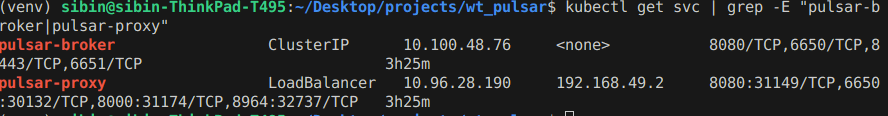
\includegraphics[width=0.8\textwidth]{implementation/pulsar-svcs.png}
    \caption{Pulsar Kubernetes Services}
    \label{fig:kgetpods}
\end{figure}

A sample Python consumer was developed to demonstrate real-time message consumption, subscribing to a specified topic with a shared subscription type and reporting end-to-end latency:

\begin{lstlisting}[breaklines=true,basicstyle=\small\ttfamily,frame=single]
consumer = client.subscribe(TOPIC_NAME, SUBSCRIPTION_NAME,
                            consumer_type=pulsar.ConsumerType.Shared)
msg = consumer.receive(timeout_millis=5000)
\end{lstlisting}

This consumer supports real-time consumption of video, audio, or chat streams and is extensible to other topics, validating integration with the Pulsar cluster.

\begin{figure}[h!]
    \centering
    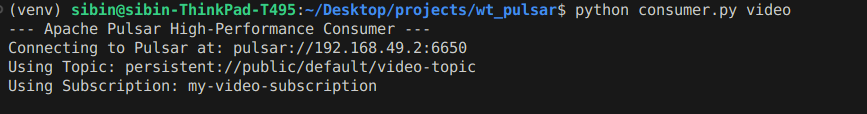
\includegraphics[width=0.8\textwidth]{implementation/consumer-video.png}
    \caption{Consumer Connection to Topic}
    \label{fig:consumer-conn}
\end{figure}

\begin{figure}[h!]
    \centering
    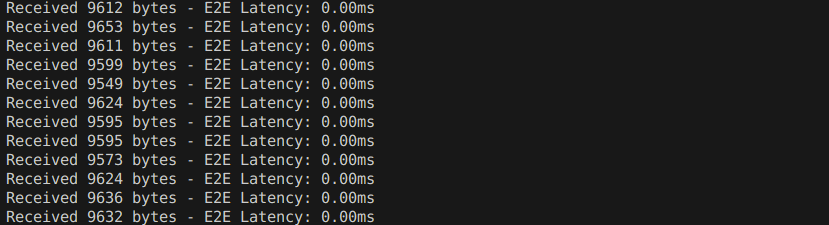
\includegraphics[width=0.8\textwidth]{implementation/pulsar-consumer-video.png}
    \caption{Consumer Receiving Data from Video Topic}
    \label{fig:consumer-data}
\end{figure}

% Describing retrieval of results
\subsection{Retrieving Results}
Metrics are logged in a CSV file within the router pod. To retrieve these files locally for evaluation, the following commands were executed:

\begin{lstlisting}[breaklines=true,basicstyle=\small\ttfamily,frame=single]
mkdir metrics-in-pod
kubectl cp webtransport-router-deployment-65cf75d584-njmqf:/app/metrics_logs ./metrics-in-pod
\end{lstlisting}

This process transfers the CSV files to the local machine, enabling detailed analysis of the system’s performance metrics.



% \section{Kubernetes Deployment}
% This implementation is the most important for the completion of our proposed solution. The router code is responsible to load balance streams of live data to seperate microservers. The router, microservice code and pulsar components are to be deployed into our kubernetes environment in minikube cluster

% \subsection{Deployment Secrets}
% To run our router in order to listen for Webtransport streams, there is a need for kubernetes to store our certficates. Certificates can be stored as secrets as detailed in Section 2.6.2, in the cluster. The generated certificate from Section 5.3 can be deployed into our kubernetes cluster so any entity in the namespace can access our certificate when mounted on a path.

% The following steps were done

% kubectl create secret tls quic-cert --cert=path/.crt --key=path/.key
% This creates a secret in kubernetes in the default namespace so all resources in the namespace can access it


% \subsection{Router Deployment}
% Router deployment was done with the steps  Containerization, creating configmaps, deployment, and service

% The router section in the implementation defines how the config file was constructed with hot reloading

% the router code was built with a docker file defined in --. This file was placed in the same directory as where the router code is and keeping the router\_config file outside. 

% docker build -t sbnm007/quic\_router:0.0.0 . 
% This built the docker image

% I pushed the docker image to dockerhub repository
% docker push sbnm007/quic\_router:0.0.0 

% Now we have successfully created a container image for our router which can be deployed to our cluster

% Firstly the router\_config file which we didnt create along with the iamge is deployed as a config map whihc allows for kubernetes managed configuration. This is a practice in k8s where parameters are put in config to allow for extensibility. In this case, the config file is used for addding or removing microservices by configuring the endpoints. This allows for change withing a single file without creating new image and avoids hard coding values. 

% The `mentioned in --router.yaml` file is a complete Kubernetes configuration that sets up the WebTransport Router, enabling it to dynamically route different types of real-time data (like video, audio, and chat) to their respective microservices. First, a `ConfigMap` is defined that contains the `router_config.yaml` (a dynamic routing configuration file that supports hot-reloading without needing to restart the router. This configuration includes routing rules for each service, such as endpoint, port, data format, and custom headers. The `Deployment` section specifies how the router is deployed inside Kubernetes, including the Docker image, ports for QUIC/HTTP3, and volume mounts for the config file and TLS certificates. It is configured to run a single replica but can be scaled up for high availability. TLS certificates are securely injected into the container using a Kubernetes `Secret`, enabling encrypted communication over QUIC. Environment variables are used by the router application to locate the mounted configuration and certificate files. Finally, the `Service` of type `LoadBalancer` exposes the router externally, allowing clients to connect via TCP or UDP on port 443. This setup ensures that the router is easily configurable, scalable, and ready for production use with secure and dynamic traffic routing capabilities.


% kubectl apply -f router.yaml
% This creates all the resources defined in the yaml
% you can check for the rources

% kubectl get pods
% kubectl get svc -> the service will receive an external ip address from the metallb



% \subsection{Microservice Deployment}

% The \texttt{microservice.yaml} file defines the complete Kubernetes configuration required to deploy the individual microservices (\textbf{video}, \textbf{audio}, and \textbf{chat}) in a scalable and dynamically configurable manner. At the core of this setup is a shared \texttt{ConfigMap} named \texttt{microservice-app-config}, which contains the \texttt{microservice\_config.yaml} file. This configuration file is mounted into each microservice container at runtime and enables hot-reloading of critical settings such as the Pulsar broker URL and toggles for enabling or disabling message forwarding to Pulsar.

% Each microservice is deployed via a dedicated \texttt{Deployment} resource, which runs a Python-based service with arguments specifying its type and listening port. The shared configuration is mounted at \texttt{/config}, and its path is provided to the container via an environment variable. This design ensures that all microservices operate independently while adhering to a consistent configuration standard.

% To facilitate internal communication within the Kubernetes cluster, each microservice is exposed via a corresponding \texttt{ClusterIP} \texttt{Service} on port \textbf{4434} for video, \textbf{4435} for audio, and \textbf{4436} for chat. This allows the WebTransport Router and other system components to route data reliably using internal DNS.

% The architecture is modular by design: new microservices can be introduced with minimal effort by replicating and modifying the relevant deployment and service blocks.

% Two key parameters in the configuration used for Pulsar integration are:

% \begin{verbatim}
% pulsar_broker_url: "pulsar://10.100.48.76:6650"
% end_to_pulsar: true
% \end{verbatim}

% These values are included in the \texttt{ConfigMap} to facilitate debugging and operational control over Pulsar connectivity.


% \subsection{Pulsar Deployment}

% Deploying Apache Pulsar within a constrained local development environment, specifically using Minikube, posed significant challenges. The official Helm chart provided in the Apache Pulsar documentation proved unsuitable in this context, primarily due to repeated out-of-memory (OOM) issues encountered in the init containers, which were followed by failures in the BookKeeper nodes.

% To address these issues, an alternative Helm chart maintained by DataStax and tailored for lightweight development environments was used. This approach facilitated a successful deployment and also enabled exposure of the Pulsar broker outside the Kubernetes cluster. The following steps summarize the installation process:

% \begin{itemize}
%     \item Add the custom Helm chart repository:
%     \begin{verbatim}
%     helm repo add datastax-pulsar https://datastax.github.io/pulsar-helm-chart
%     \end{verbatim}

%     \item Update the Helm repository to fetch the latest charts:
%     \begin{verbatim}
%     helm repo update
%     \end{verbatim}

%     \item Download the example development configuration:
%     \begin{verbatim}
%     curl -LOs https://datastax.github.io/pulsar-helm-chart/examples/dev-values.yaml
%     \end{verbatim}

%     \item Modify \texttt{dev-values.yaml} to disable monitoring by setting:
%     \begin{verbatim}
%     kube-prometheus-stack:
%       enabled: false
%     \end{verbatim}
%     This change was essential to reduce resource consumption and ensure stability on limited hardware.

%     \item Deploy Pulsar with the modified configuration:
%     \begin{verbatim}
%     helm install pulsar -f dev-values.yaml datastax-pulsar/pulsar
%     \end{verbatim}
% \end{itemize}

% This deployment results in two essential services: \texttt{pulsar-broker}, which provides the internal message brokering functionality, and \texttt{pulsar-proxy}, which facilitates external access to the Pulsar ecosystem. 

% \begin{figure}[h!]
%     \centering
%     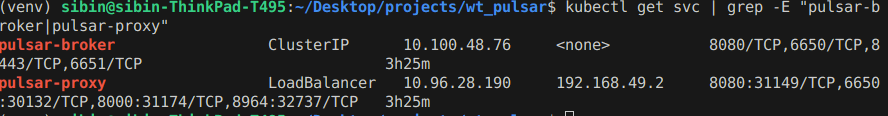
\includegraphics[width=0.8\textwidth]{implementation/pulsar-svcs.png}
%     \caption{Pulsar K8s Services}
%     \label{fig:kgetpods}
% \end{figure}



% For in-cluster applications such as the microservices discussed earlier, communication with Pulsar occurs via the ClusterIP of the \texttt{pulsar-broker}. This enables efficient internal streaming to topics hosted within the Kubernetes network.

% For external consumers, connectivity is established via the \texttt{pulsar-proxy}, whose endpoint is exposed using a MetalLB load balancer. This approach ensures that consumers outside the Kubernetes cluster can access Pulsar using a stable IP address.

% A sample Python consumer was developed to demonstrate real-time message consumption. The consumer subscribes to a specified topic using a shared subscription type and reports end-to-end latency for each received message. The connection parameters, such as topic name and subscription identifier, are passed as command-line arguments.

% \begin{verbatim}
% consumer = client.subscribe(TOPIC_NAME, SUBSCRIPTION_NAME,
%                             consumer_type=pulsar.ConsumerType.Shared)
% msg = consumer.receive(timeout_millis=5000)
% \end{verbatim}

% This consumer architecture supports multiple use cases, including the real-time consumption of video, audio, or chat streams, and can be extended to other topics as required. It validates the successful integration between external clients and the Pulsar cluster deployed within Kubernetes.

% # image of consumption
% \begin{figure}[h!]
%     \centering
%     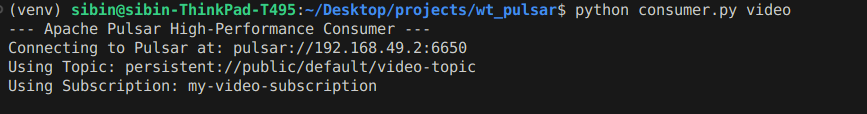
\includegraphics[width=0.8\textwidth]{implementation/consumer-video.png}
%     \caption{Consumer connection to topic}
%     \label{fig:consumer-conn}
% \end{figure}

% \begin{figure}[h!]
%     \centering
%     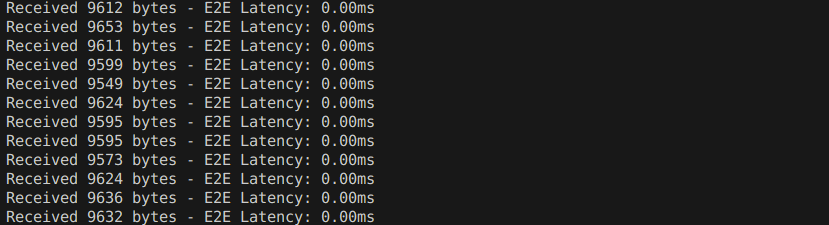
\includegraphics[width=0.8\textwidth]{implementation/pulsar-consumer-video.png}
%     \caption{Consumer Receiving Data from Video Topic}
%     \label{fig:consumer-data}
% \end{figure}




% \subsection{Getting the results}

% The CSV file is being logged inside the pod which captures our detailed metrics The following command is run to fetch the csv file to our local system
% mkdir metrics-in-pod
% kubectl cp webtransport-router-deployment-65cf75d584-njmqf:/app/metrics_logs ./metrics-in-pod
% With this we get the csv files in our local machien which we can evaluate

% \subsection{Pulsar Deployment}
% This part was particularly complex. I could not use the existing helm chart available in Apache Pulsar documentation. I faced issue where my init containers were giving OOM followed by bookie failure. I used alternative installation mechanism specifically for minikube by following the following steps

% Due to resource constaints I faced several challenges where my machine would go out of memory.
% I followed installation with this specific helm chart which made it work also helped to expose kafka broker out of kubernetes. 

% I ran the following commands
% This adds the custom chart  repo
% helm repo add datastax-pulsar https://datastax.github.io/pulsar-helm-chart

% helm repo update
% This gets the values.yaml file to my machine
% curl -LOs https://datastax.github.io/pulsar-helm-chart/examples/dev-values.yaml
% In this values.yaml I disable monitoring by setting kube-prometheus-stack: enabled : false so as to make my solution more efficient. 
% This applies the configuration and sets up our event broker service
% helm install pulsar -f dev-values.yaml datastax-pulsar/pulsar 

% This helm chart sets up pulsar-proxy as well as pulsar-broker 2 services which exposes end point for us to interact with apache pulsar. In this for our application code deployed in kuberentes we will use the cluster ip of the broker which allows us to push streams to respective topics within k8s


% For consumers sitting outside of pulsar, I will connect using pulsar-proxy endpoint which gets the ip address from my metal-lb load balancer.

% The consumer is a python code which connections to specified topic taken as command line arguments with new subscription. It also measures the end to end latency observed and successfully consumes the streams.

% % \\code
% % consumer = client.subscribe(TOPIC_NAME, SUBSCRIPTION_NAME, consumer_type=pulsar.ConsumerType.Shared)
% % msg = consumer.receive(timeout_millis=5000)


% Outside of my kubernetes cluster I consumers, this creates a subscription and connect to the respected pulsar topics and can consume respective streams in real-time. Following is the example of a consumer consuming from video topic

% 






% \section{Summary}

% The implementation began by setting up a local Kubernetes environment using Minikube with MetalLB for LoadBalancer functionality. TLS support was configured through self-signed certificates mapped to a custom domain, allowing secure WebTransport connections. A browser-based WebTransport client was built to stream multiple data types including video, audio, chat, files, and screen shares, each over distinct unidirectional QUIC streams. The client features a custom packet header format, real-time UI with live logs, and performance metrics. Wireshark was configured to decrypt QUIC traffic for validation using Chrome’s session keys.

% The WebTransport router, implemented in Python using aioquic, supports asynchronous QUIC + HTTP/3 stream handling, per-stream buffering, dynamic routing via a YAML config, and metrics logging. It forwards packets to generic microservices through a proxy layer. Each microservice processes packets based on type and can dynamically publish to Apache Pulsar using configurable producers and topic mapping. Pulsar was deployed with optimized Helm chart settings from DataStax to ensure stable operation in constrained local environments. Overall, the system successfully enables real-time multimedia streaming, processing, and message queuing, all managed within a fully containerized and configurable Kubernetes deployment.



\section{Network Traffic Analysis}
With both the WebTransport client and router implemented and deployed, this section demonstrates the actual network traffic captured during live streaming sessions. Using Wireshark with the previously configured TLS decryption, we can observe the real-time communication between the client and router, validating the implementation and providing insights into the protocol behavior.
\begin{figure}[h]
    \centering
    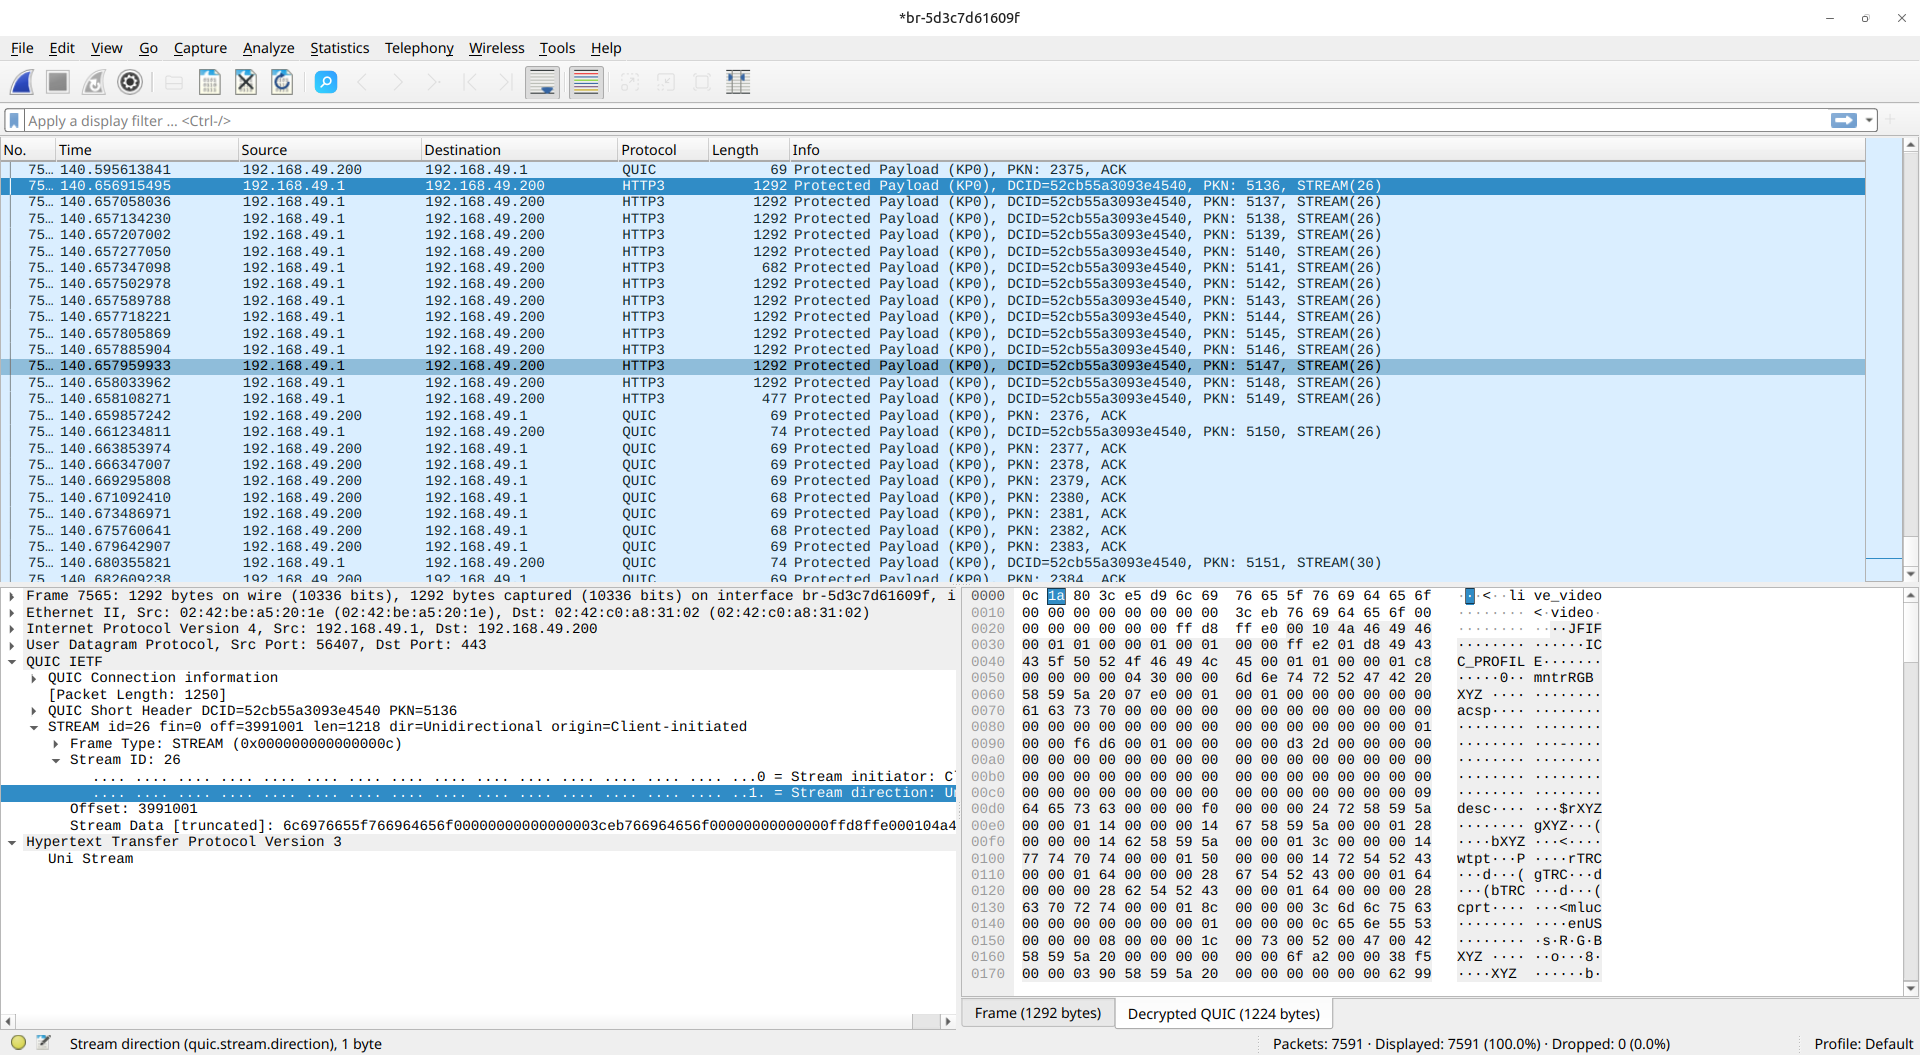
\includegraphics[width=0.8\textwidth]{implementation/network_traffic_analysis.png}
    \caption{Network Traffic Analysis using Wireshark}
    \label{fig:network_traffic_analysis}
\end{figure}


The figure \ref{fig:network_traffic_analysis} shows a snapshot of the network traffic captured on the 'br-5d3c7d61609f' network interface, which is where the custom router is deployed within the Kubernetes cluster. The source IP address 192.168.49.1 represents the WebTransport client, while the destination IP address 192.168.49.200 corresponds to the router's IP address exposed through MetalLB with a custom configured domain name.

The highlighted stream 26 demonstrates the HTTP/3 protocol implementation, with stream number 26 specifically handling live video data. Upon examining the decrypted QUIC packet in the bottom right panel, the packet structure begins with the expected 32-byte header containing the track identifier is correctly set to 'live\_video' as shown in the figure. The subsequent streams represent fragmented packets of the same stream type (live\_video), all maintaining the consistent stream ID 26, which validates the proper stream multiplexing implementation.

This captured traffic successfully validates the implementation of both the WebTransport client and router, demonstrating the successful transmission and processing of live video data. The network capture also reveals audio and chat packets transmitted over stream IDs 30 and 22 respectively, confirming the multi-stream architecture where different media types are isolated into separate streams to prevent head-of-line blocking.





\section{Summary}

In this chapter, a complete end-to-end prototype of the proposed system is implemented and validated within a local Kubernetes environment. The workflow begins with a browser-based WebTransport client that streams multiple types of media, such as video, audio, chat, and files in real time using unidirectional QUIC streams. Each packet is formatted with a custom header and transmitted securely using TLS, with certificate handling and DNS mapping configured for seamless local development. The system demonstrates robust session management, live metrics collection, and a responsive user interface, enabling detailed insight into the streaming behavior.

The WebTransport router, deployed as a scalable microservice, acts as the central intelligence for traffic distribution. It uses asynchronous QUIC and HTTP/3 handling to buffer, parse, and dynamically route packets to the appropriate microservices based on a hot-reloadable YAML configuration. These backend microservices, implemented generically to support various media types, process the data and optionally publish it to Apache Pulsar topics for further stream processing or analytics. The deployment showcases critical infrastructure features such as TLS termination, local DNS resolution, zero-downtime scaling, and runtime observability, all orchestrated through Minikube, MetalLB, and Kubernetes-native tools. This working prototype not only verifies the architectural design but also lays a strong, extensible foundation for production-scale deployments or future research-driven enhancements.
% \chapter{Evaluation}
% \label{chap:Evaluation}

% This chapter discusses about the methods of evaluation that are performed to extensively evaluate our solutiom. Evaluation is performed on the core component of our proposed solution which is custom router within kubernetes. 

% For evaluation, unlike normal http servres where we expose a /metrics endpoint for capturing real-time metrics through prometheus grafana is the practice in todays time. We are dealing with a HTTP3 server where support lacks. The solution could be to run 2 servers simultaneously but it would be not feasible. The alternative to evaluation was used where a logging mechanism was done to a csv file


% \section{Experiments}
% The following are the experiments which are performed on the router server

% single client performance on router and machine
% multiple clients (3) performance on router and machine
% higher MTU performance on router and machine
% The following metrics were considered for performance evaluation

% Buffer Metrics: buffer_size_bytes, max_buffer_size_bytes, buffer_overflows | Packet Processing: packets_total, packets_complete, packets_fragmented, fragmentation_rate | Stream Management: streams_active, streams_max_concurrent | Performance: throughput_mbps, avg_processing_time_ms, avg_buffer_wait_ms | Identification: timestamp, client_id

% With these metrics 




% For the experimental setup, the solutions were monitored in kubernetes with kubectl logs giving the live metrics. Code changes were done to create a csv file with the detailed metrics mentioned above. These are the values which were set for the experiments 

% #Create Table
% \begin{table}[h!]
% \centering
% \caption{Router Constants}
% \begin{tabular}{|l|l|l|}
% \hline
% \textbf{Parameter} & \textbf{Default Value} & \textbf{Description} \\
% \hline
% \texttt{max-data} & 1048576 (1MB) & Maximum amount of unacknowledged data for the entire connection. \\
% \hline
% \texttt{max-stream-data} & 262144 (256KB) & Maximum amount of unacknowledged data for each individual stream. \\
% \hline
% \texttt{max-datagram-size} & 3000 (bytes) & Maximum size for a single datagram/packet. \\
% \hline
% Buffer overflow threshold & 10MB & The size at which a buffer is considered to be overflowing. \\
% \hline
% Large buffer detection & 5MB & The size at which a buffer is detected as being large. \\
% \hline
% High fragmentation threshold & 0.5 (50\%) & The fragmentation rate considered to be high. \\
% \hline
% High stream count threshold & 10 streams & The number of streams considered to be high. \\
% \hline
% Sample retention limit & 1000 samples & The maximum number of samples to retain. \\
% \hline
% Default timeout & 30 seconds & The default timeout for a request. \\
% \hline
% Default retries & 3 & The default number of retries for a request. \\
% \hline
% Default connect timeout & 5 seconds & The default timeout for establishing a connection. \\
% \hline
% Default content type & "application/octet-stream" & The default content type for a request. \\
% \hline
% \end{tabular}
% \end{table}


% \begin{table}[h!]
% \centering
% \caption{Router Constants}
% \begin{tabular}{|l|l|l|}
% \hline
% \textbf{Parameter} & \textbf{Default Value} & \textbf{Description} \\
% \hline
% \texttt{max-data} & 1048576 (1MB) & Maximum amount of unacknowledged data for the entire connection. \\
% \hline
% \texttt{max-stream-data} & 262144 (256KB) & Maximum amount of unacknowledged data for each individual stream. \\
% \hline
% \texttt{max-datagram-size} & 3000 (bytes) & Maximum size for a single datagram/packet. \\
% \hline
% Buffer overflow threshold & 10MB & The size at which a buffer is considered to be overflowing. \\
% \hline
% Large buffer detection & 5MB & The size at which a buffer is detected as being large. \\
% \hline
% High fragmentation threshold & 0.5 (50\%) & The fragmentation rate considered to be high. \\
% \hline
% High stream count threshold & 10 streams & The number of streams considered to be high. \\
% \hline
% Sample retention limit & 1000 samples & The maximum number of samples to retain. \\
% \hline
% Default timeout & 30 seconds & The default timeout for a request. \\
% \hline
% Default retries & 3 & The default number of retries for a request. \\
% \hline
% Default connect timeout & 5 seconds & The default timeout for establishing a connection. \\
% \hline
% Default content type & "application/octet-stream" & The default content type for a request. \\
% \hline
% \end{tabular}
% \end{table}

% \vspace{1cm}

% \begin{table}[h!]
% \centering
% \caption{Media Parameters}
% \begin{tabular}{|l|l|l|}
% \hline
% \textbf{Parameter} & \textbf{Value} & \textbf{Description} \\
% \hline
% STANDARD\_VIDEO\_FPS & 15 & Standard video frame rate in packets per second. \\
% \hline
% HIGH\_VIDEO\_FPS & 30 & High video frame rate in packets per second. \\
% \hline
% AUDIO\_BUFFER\_SIZE & 4096 & Number of samples per audio packet. \\
% \hline
% PACKET\_HEADER\_SIZE & 32 & Total size of the packet header in bytes. \\
% \hline
% TRACK\_ID\_SIZE & 16 & Size of the track ID in bytes. \\
% \hline
% PAYLOAD\_LENGTH\_SIZE & 4 & Size of the payload length field in bytes. \\
% \hline
% TRACK\_TYPE\_SIZE & 12 & Size of the track type field in bytes. \\
% \hline
% STANDARD\_VIDEO\_QUALITY & 0.7 & Standard video quality (lower compression). \\
% \hline
% HIGH\_VIDEO\_QUALITY & 0.9 & High video quality (higher compression). \\
% \hline
% \end{tabular}
% \end{table}

% \vspace{1cm}

% \begin{table}[h!]
% \centering
% \caption{Webtransport Client Constants}
% \begin{tabular}{|l|l|l|}
% \hline
% \textbf{Parameter} & \textbf{Value} & \textbf{Description} \\
% \hline
% STANDARD\_VIDEO\_FPS & 15 & Standard video frame rate in packets/second. \\
% \hline
% HIGH\_VIDEO\_FPS & 30 & High video frame rate in packets/second. \\
% \hline
% AUDIO\_BUFFER\_SIZE & 4096 & Audio samples per packet. \\
% \hline
% PACKET\_HEADER\_SIZE & 32 & Total size of the packet header in bytes. \\
% \hline
% TRACK\_ID\_SIZE & 16 & Size of the track ID in bytes. \\
% \hline
% PAYLOAD\_LENGTH\_SIZE & 4 & Size of the payload length in bytes. \\
% \hline
% TRACK\_TYPE\_SIZE & 12 & Size of the track type in bytes. \\
% \hline
% STANDARD\_VIDEO\_QUALITY & 0.7 & Standard video quality (lower compression). \\
% \hline
% HIGH\_VIDEO\_QUALITY & 0.9 & High video quality (higher compression). \\
% \hline
% \end{tabular}
% \end{table}

% These values are kept constant to extensively evaluate the defined experiments



% In the case where experiments have been carried out, the experimental setup and the values that were defined for the variables need to be presented in a table e.g. table~\ref{tab:experimentsetup}.


% \section{Results}


% ### Chapter 6: Evaluation

% #### 6.1 Single Client Analysis – *Client ID: 134311891535872*

% This section presents an in-depth analysis of the system performance during a WebTransport session with a single client, identified as `client_134311891535872`. The session lasted approximately 140 seconds, starting from `2025-08-03T21:39:38` and concluding at `2025-08-03T21:41:58`, with a final termination observed at `21:42:03`. Key performance metrics collected include total packet count (`packets_total`), fragmented packets (`packets_fragmented`), fragmentation rate, throughput in megabits per second (`throughput_mbps`), current and maximum buffer size (`buffer_size_bytes`, `max_buffer_size_bytes`), average processing time (`avg_processing_time_ms`), and average buffer wait time (`avg_buffer_wait_ms`).

% The system showed overall stability throughout the session. A consistently high fragmentation rate of approximately 0.87 was recorded, yet this did not negatively affect throughput or latency. Throughput was stable in the range of 0.47 to 0.50 Mbps, and latency remained impressively low, with average processing and buffer wait times of 0.03 milliseconds. Importantly, no buffer overflows were observed, indicating effective buffer management despite load variability.

% ##### 6.1.1 Packet Processing and Fragmentation

% The total number of packets processed grew steadily until it reached 41,942 at around 21:41:33, after which no additional packets were recorded, coinciding with session termination. The fragmentation rate stabilized at approximately 0.869 to 0.870, with a total of 36,488 fragmented packets. Compared to other clients analyzed in the dataset, this rate is higher than that of client `134311831858512` (0.865), but lower than clients `134311834991552` and `134311831849104` which experienced fragmentation rates nearing 0.892.

% Despite the relatively high fragmentation, system performance did not degrade. Throughput and latency remained unaffected, suggesting robust handling of packet fragmentation by the underlying protocol and system design. Nevertheless, the presence of frequent `HIGH_FRAGMENTATION` log messages indicates that the system recognizes this condition as potentially problematic and warrants further investigation or future optimization.

% ##### 6.1.2 Throughput Analysis

% The throughput for this session ranged from 0.4657 to 0.5007 Mbps, reaching its peak at approximately 21:40:53. A gradual decline followed, culminating in a drop to 0.0 Mbps by 21:41:38. This decline coincides with the cessation of packet activity and indicates a smooth and expected shutdown of the connection.

% In comparative terms, the client's throughput is consistent with client `134311831858512`, whose throughput ranged from 0.5 to 0.6 Mbps. Moreover, it outperformed clients `134311834991552` and `134311831849104`, both of which maintained average throughputs closer to 0.3 Mbps. This suggests that the system maintains throughput efficiently even when managing higher fragmentation rates.

% ##### 6.1.3 Buffer Utilization

% Buffer usage exhibited occasional spikes, such as a notable increase to 9,940 bytes at 21:40:13. The maximum recorded buffer size was 17,214 bytes, which is significantly lower than the 85,937 bytes observed in client `134311831858512`. This reduced buffer size correlates with a lower total packet count and implies reduced strain on the buffer system during this session.

% The absence of buffer overflows further supports the conclusion that the system's buffer management strategy is effective, even under dynamic conditions. These observations point toward a well-balanced buffering approach that maintains operational integrity while accommodating varying packet flows.

% ##### 6.1.4 Processing and Latency Metrics

% The metrics for average processing time and average buffer wait time both remained stable at 0.03 milliseconds. These figures were consistent across the session and did not show any significant correlation with variations in throughput or fragmentation.

% Compared with other clients, these values fall within the expected range of 0.02 to 0.03 milliseconds, indicating a reliable and low-latency processing pipeline. This consistent performance underscores the effectiveness of the system’s internal processing mechanisms and reaffirms its suitability for real-time transport applications.

% ##### 6.1.5 Connection Termination

% The WebTransport session concluded at 21:42:03, marking the end of active data transmission. Notably, `throughput_mbps` dropped to 0.0 Mbps at 21:41:38, and log entries continued until 21:41:58. The persistence of `HIGH_FRAGMENTATION` messages until the session's end suggests a possible link between fragmentation and early termination.

% The session duration of 140 seconds is shorter than the average 180-second sessions observed with other clients. This discrepancy might indicate a client-initiated termination, a network timeout, or an internal system limit. Further analysis involving external logs and client-side diagnostics would be necessary to determine the exact cause.

% ##### 6.1.6 System Resource Utilization

% System resource consumption was measured using the `top` utility on the host machine, a ThinkPad T495. The WebTransport router pod (`webtransport-router-deployment-65cf75d584-njmqf`) exhibited CPU usage ranging from 273m (0.273 cores) to 560m (0.56 cores), and memory usage ranging from 27MiB to 72MiB.

% These values indicate a lightweight and resource-efficient implementation, with sufficient headroom for scaling under heavier workloads. The fluctuations observed likely reflect periodic spikes in activity or preparation for graceful termination.

% ##### 6.1.7 Summary and Recommendations

% The session displayed stable throughput, minimal latency, and effective buffer management. However, the following recommendations are proposed:

% * **Investigate the root cause of the early termination**, which may stem from network issues or configuration limits.
% * **Optimize fragmentation behavior** to reduce the rate toward 0.865, aligning it with the lower-bound observed in other clients.
% * **Monitor buffer activity** during future sessions to preemptively identify bottlenecks or inefficiencies.
% * **Conduct configuration comparisons** with high-performing clients such as `134311831858512` to extract tuning parameters.

% ##### 6.1.8 Limitations

% This evaluation is based on a single client session, limiting the scope for broader conclusions about multi-client behavior. The relatively short session duration may not capture long-term trends or degradation. Additionally, the constancy of latency metrics reduces the opportunity for in-depth correlation analysis. The absence of external logs further restricts the ability to pinpoint causes of fragmentation or termination events.

% ---

% #### 6.2 Multi-Client Comparison

% To place the findings from `client_134311891535872` into context, a comparative analysis was conducted using data from three other clients: `client_134311831858512`, `client_134311834991552`, and `client_134311831849104`. Each of these clients had longer sessions of approximately 180 seconds, enabling a more robust evaluation of trends over time.

% From a packet volume perspective, the target client processed 41,942 packets, which is significantly lower than the 95,431 packets processed by `client_134311831858512` but comparable to the other two clients, who handled between 45,401 and 47,195 packets. The fragmentation rate of 0.87 places the target client between the low-fragmentation client (`134311831858512`, 0.865) and the high-fragmentation clients (\~0.892).

% In terms of throughput, the target client's rate of 0.47–0.50 Mbps aligns closely with the best-performing client and significantly surpasses the lower throughput clients, whose performance hovered around 0.3 Mbps. This suggests that throughput is maintained effectively despite moderate fragmentation.

% Buffer usage was also notably lower, with a maximum buffer size of 17,214 bytes, compared to the 85,937 bytes recorded for the high-volume client. This reflects the lower packet volume and reduced buffer strain.

% Resource usage also favored the target client. With CPU consumption between 273m and 560m, and memory between 27MiB and 72MiB, the system demonstrated efficient resource utilization. This further supports the scalability of the current design for multi-client workloads.

% ---





% \includescalefigure{fig:measurements}{Measurement of System Wakeups}{Long caption that describes the figure to the reader}{1}{measurements.png}


% Figures that present results such as figure~\ref{fig:measurements} need to display descriptions of the axes, the units and scales of the measurements, statistical values, etc. Where measurements were taken from experiments, error bars or confidence intervals need to be provided to give the reader an indication of the spread of the measurements.



% \section{Summary}
% The evaluation of client `134311891535872` demonstrates that the implemented WebTransport router is capable of delivering consistent performance under moderately loaded conditions. The system maintained stable throughput levels (0.47–0.50 Mbps), handled a moderate fragmentation rate (\~0.87) without degrading performance, and sustained low-latency operation throughout the session.

% Buffering and system resource metrics confirm a robust and efficient architecture. Notably, this client achieved comparable throughput to higher-volume clients while consuming fewer resources and generating fewer packets. These attributes suggest a well-tuned design capable of scaling to more complex and concurrent deployments.

% Nonetheless, the presence of persistent fragmentation and early session termination highlights areas for further investigation and optimization. Future work should focus on reducing fragmentation, extending session stability, and enhancing monitoring capabilities to better understand the interaction between system events and performance outcomes.



\chapter{Evaluation}
\label{chap:Evaluation}

This chapter presents a comprehensive evaluation of the WebTransport-aware routing system deployed on Minikube \cite{minikube-docs}. The evaluation focuses on performance metrics including latency, throughput, and resource utilization under different client loads and network conditions.

The WebTransport stream routing system's evaluation in kubernetes has been thoroughly evaluated in this chapter. The analysis is aimed at assessing the performance, scalability, custom router features and reliability by evaluating under different load conditions.  Monitoring solutions like Prometheus and Grafana are not used here because of this system being an HTTP/3 server and the custom monitoring not supporting it. This system follows the use of a different approach because of limited tooling support for Webtransport protocol. Our HTTP/3 WebTransport server follows a procedure that allows the capture of the detailed performance metrics in Comma-Separated Values (CSV) format.

The evaluation method includes both measuring qualitative as well as quantitative performance. This helps us understand what the system can do well and where it might have limitations when used in real-world environments.


\section{Experimental Design}

The evaluation of the WebTransport-aware routing system requires a comprehensive experimental framework that validates both functional correctness and performance characteristics under varying load conditions. This section outlines the systematic approach taken to assess the system's capabilities, including the methodology for metrics collection, the specific experimental configurations used to simulate real-world scenarios, and the rationale behind the chosen evaluation parameters. The experimental design ensures that the assessment covers critical aspects such as latency, throughput, fragmentation handling, and resource utilization across different client load scenarios.

\subsection{Evaluation Methodology}

The evaluation methodology employs a multi-dimensional metrics collection system designed to capture comprehensive performance characteristics across four critical parts. The Buffer Management Metrics provide insights into memory utilization patterns through `buffer\_size\_bytes`, which tracks real-time buffer consumption whereas `max\_buffer\_size\_bytes` records peak memory usage during sessions. Similarly, `buffer\_overflows` counts critical overflow events that could indicate system stress or inadequate resource allocation. 

Packet Processing Metrics forms the core for performance analysis, it has `packets\_total` which is for aggregate packet volume, `packets\_complete` represents successfully processed packets without fragmentation, `packets\_fragmented` indicates packets requiring segmentation due to size constraints, and `fragmentation\_rate` expressing the percentage of packets experiencing fragmentation which acts as a critical indicator of network efficiency and potential performance bottlenecks.

Stream Management Metrics monitors the multiplexing capabilities of to WebTransport streams by measuring `streams\_active`, which tracks currently operational streams, and `streams\_max\_concurrent`, which records the peak simultaneous stream count which is useful for testing the upper limit. Finally, Performance Metrics quantifies system responsiveness and efficiencies via `throughput\_mbps` metric which measures data transmission rates in megabits per second, `avg\_processing\_time\_ms`, captures the mean latency for packet processing operations, and `avg\_buffer\_wait\_ms`, indicates queuing delays within the buffer management system. 

These comprehensive metrics enables granular analysis of system behavior under varying load conditions, allowing us to identify bottlenecks, establish faster debugging, analyze resource utilization patterns, and optimization opportunities essential for validating the WebTransport router’s operational effectiveness for production grade Kubernetes environments.


\subsection{Experimental Configuration}
The experimental setup used the following configuration parameters to ensure reproducible results across all test scenarios and to understand the router specific performance.

\begin{table}[h!]
\centering
\caption{Router Configuration Parameters}
\label{tab:router-config}
\renewcommand{\arraystretch}{1.3} % Increases row spacing for better readability
\begin{tabular}{|l|l|}
\hline
\textbf{Parameter} & \textbf{Value} \\
\hline
\texttt{max-data} & 1048576 (1MB) \\
\hline
\texttt{max-stream-data} & 262144 (256KB) \\
\hline
\texttt{max-datagram-size} & 3000 bytes\\
\hline
Buffer overflow threshold & 10MB\\
\hline
Large buffer detection & 5MB \\
\hline
High fragmentation threshold & 0.5 (50\%) \\
\hline
Sample retention limit & 1000 samples \\
\hline
Default timeout & 30 seconds  \\
\hline
Default retries & 3 \\
\hline
Default connect timeout & 5 seconds \\
\hline
\end{tabular}
\end{table}

The `--max-data` parameter (1GB) sets the total unacknowledged data limit for the entire QUIC connection. This value is chosen to support high-throughput streaming without risking excessive memory use for pod in kubernetes. The `--max-stream-data` value (256KB) caps unacknowledged data per stream to ensure a balance between throughput and fairness across multiple concurrent streams. The `--max-datagram-size` (3000 bytes) is selected to minimize packet fragmentation while remaining within typical MTU limits. These values closely follow or slightly adjust the default settings provided by `aioquic` to better fit the memory and latency characteristics of the deployment environment. The buffer overflow threshold prevents excessive memory usage, since we are running the pod in kubernetes, the pod memory limits could crash the system hence a 10MB limit. It also has a mechanism which detects large buffers at 5MD threshold so we can receive alerts with logs before the buffer overflows. This helps to monitor when buffer grows unusually large. A threshold is set of 0.5 for fragmentation to identify the extent of fragmentation. Its calculated by dividing the observed fragmented packets by total packets.The timeout parameters ensure robust connection handling by allowing 30 seconds for requests and 3 retries before failure, preventing resource exhaustion from stalled connections.  
A 5-second connect timeout balances responsiveness with reliability, tuned for typical Kubernetes network conditions under variable load.


\begin{table}[h!]
\centering
\caption{Video Quality Configuration}
\label{tab:video-quality}
\renewcommand{\arraystretch}{1.3}
\begin{tabular}{|l|l|}
\hline
\textbf{Parameter} & \textbf{Value} \\
\hline
FPS & 15 fps \\
\hline
Resolution & 640x480 \\
\hline
Compression & 0.7 \\
\hline
\end{tabular}
\end{table}

\begin{table}[h!]
\centering
\caption{Audio Configuration}
\label{tab:audio-config}
\renewcommand{\arraystretch}{1.3}
\begin{tabular}{|l|l|}
\hline
\textbf{Parameter} & \textbf{Value} \\
\hline
Buffer Size & 4096 samples \\
\hline
Channels & 1 (mono) \\
\hline
PCM Range & -32768 to 32767 \\
\hline
\end{tabular}
\end{table}

\begin{table}[h!]
\centering
\caption{Packet and Track Configuration}
\label{tab:packet-track-config}
\renewcommand{\arraystretch}{1.3}
\begin{tabular}{|l|l|}
\hline
\textbf{Parameter} & \textbf{Value} \\
\hline
\multicolumn{2}{|c|}{\textbf{Packet Structure}} \\
\hline
Header Size & 32 bytes \\
\hline
Track ID Size & 16 bytes \\
\hline
Payload Length Size & 4 bytes \\
\hline
Track Type Size & 12 bytes \\
\hline
\multicolumn{2}{|c|}{\textbf{Track IDs}} \\
\hline
Live Video & 'live\_video' \\
\hline
Live Audio & 'live\_audio' \\
\hline
Live Chat & 'live\_chat' \\
\hline

\multicolumn{2}{|c|}{\textbf{Track Types}} \\
\hline
Video Type & 'video' \\
\hline
Audio Type & 'audio' \\
\hline
Chat Type & 'chat' \\
\hline
\end{tabular}
\end{table}

The WebTransport client is constructed with the conservative performance options that allows for consistent results and guarantee a very wide compatibility and that streaming performance across diverse network conditions and devices. The video streaming is set to 15 fps in 640x480 resolution with 0.7 JPEG compression which is a reasonable compromise between visual quality and bandwidth consumptions.Audio processing is buffered internally with a 4096-sample (in mono) size at 16-bit PCM encoding to provide about 93ms of audio latency at common 44.1 kHz sampling frequencies which enough to provide good real-time performance without excessive processing overhead. The system uses three separate and unidirectional streams (live\_video, live\_audio, live\_chat) to allow effective multiplexing and flow control on a per-media-type basis.

The client uses a custom format of 32 bytes of fixed-size fields as packet header which helps WebTransport router efficiently parse the packet: 16 bytes of stream identification, 4 bytes of payload length, and 12 bytes for classifying a track type. This well-ordered design enables the router to forward packets into proper microservices. The track type system ('video', 'audio', 'chat') provides clear semantic routing information, while the fixed header size aligns with memory boundaries for good processing performance. These default parameters create a evaluation friendly system that generates measurable buffer dynamics and fragmentation patterns essential for this dissertation

\section{Results and Analysis}
In order to observe reliable results the the experiments ie single client and multi Client tests were run for a total duration of 10 minutes in order to observe the performance over time with the configurations defined in section.

\subsection{Single Client Performance Analysis}

The single client experiment provides baseline performance characteristics of the WebTransport router under minimal load conditions.
\begin{figure}[h!]
\centering
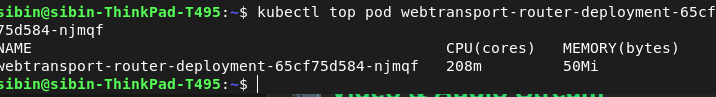
\includegraphics[width=0.8\textwidth]{Evaluation/new-single-client-stats.png}
\caption{Single Client Router Performance Overview}
\label{fig:single-client-overview}
\end{figure}

Figure~\ref{fig:single-client-overview} demonstrates the overall router pod performance during single client operation, showing stable resource utilization and consistent processing patterns.

\begin{figure}[h!]
\centering
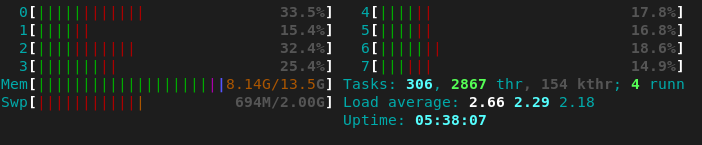
\includegraphics[width=0.8\textwidth]{Evaluation/single-client-host-stats.png}
\caption{Single Client Host Machine Performance Overview}
\label{fig:single-client-host-overview}
\end{figure}
Figure~\ref{fig:single-client-host-overview} demonstrates the impact on the overall host machine performance during single client operation.



\subsubsection{Packet Processing Performance}

\begin{figure}[h!]
\centering
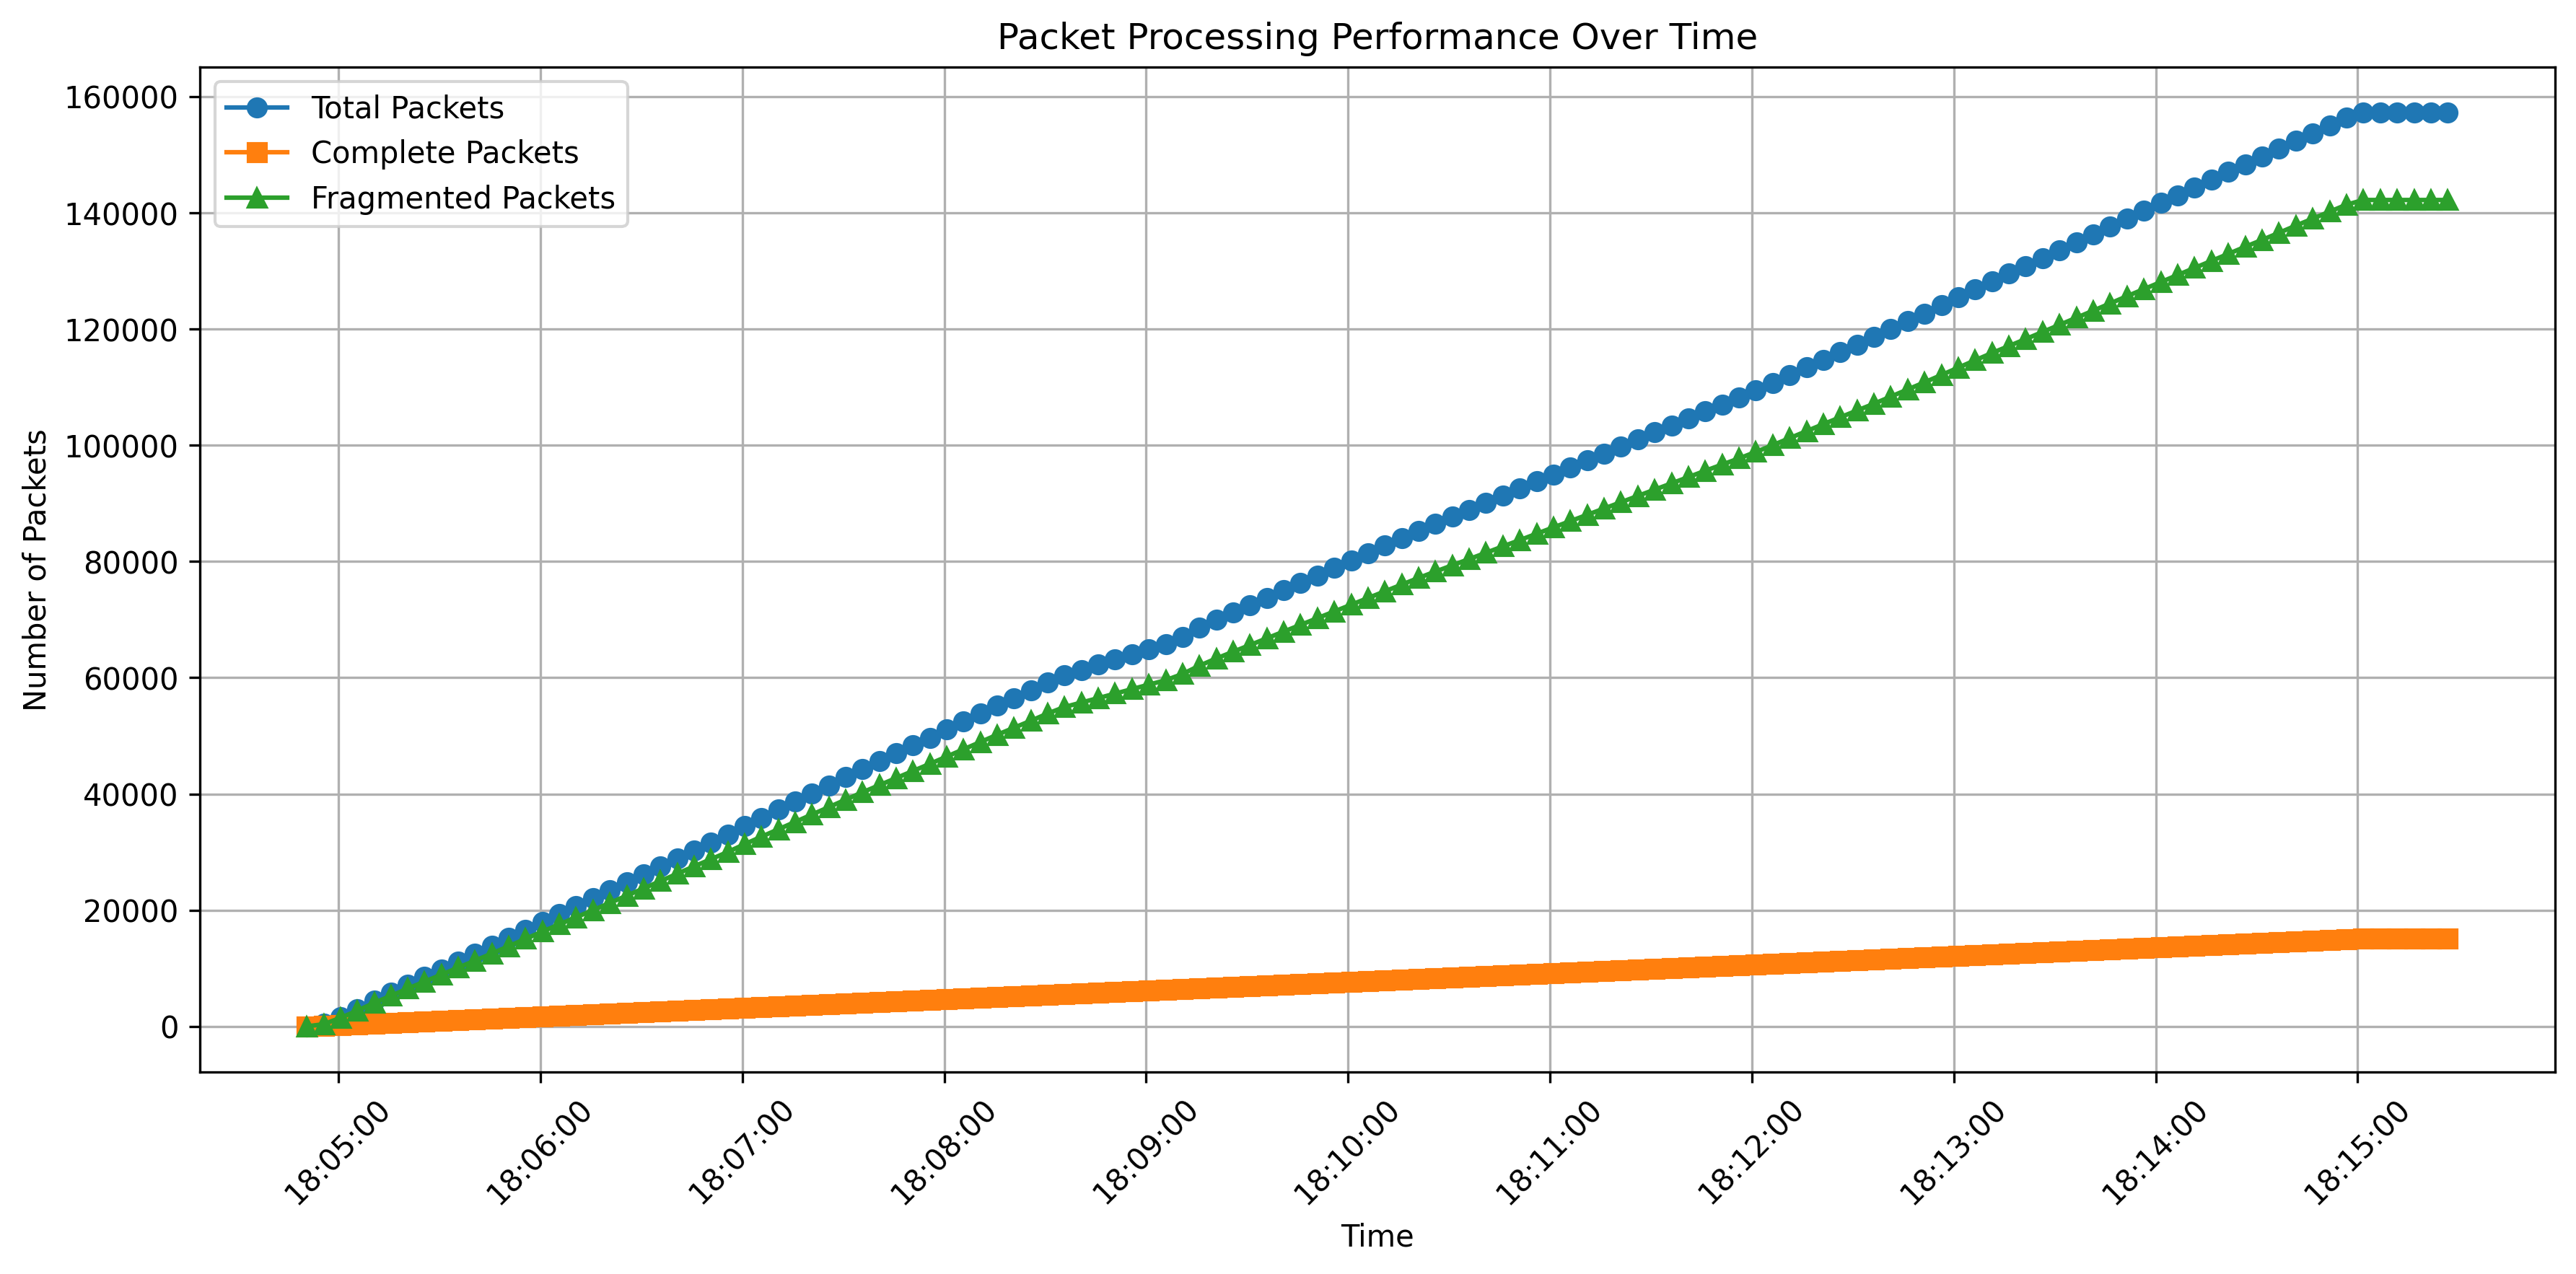
\includegraphics[width=0.8\textwidth]{Evaluation/single_packet_processing_performance.png}
\caption{Single Client Packet Volume vs Time}
\label{fig:single-packet-performance}
\end{figure}

Figure~\ref{fig:single-packet-performance} presents the packet processing performance from 18:05 to 18:15, during which the system handled a total of 157,285 packets. Throughout this 10-minute window, packet processing exhibited a consistent linear growth rate, indicating stable system performance without any observable bottlenecks. Notably, the fragmentation rate stabilized at approximately 90.4\%, corresponding to 142,233 fragmented packets. This high fragmentation ratio suggests that the majority of incoming packets exceeded the configured maximum datagram size, likely due to the nature of the input streams. In contrast, only 15,052 complete packets were received, forming a small but steady subset of the total traffic. All fragmented packets were successfully reassembled, achieving a 100\% reconstruction rate. Furthermore, system throughput peaked at around 0.3385 Mbps and remained stable, while processing and buffer wait times consistently averaged between 0.03 and 0.04 milliseconds, demonstrating the system's efficiency in managing high-throughput, fragmented traffic.


\subsubsection{Fragmentation Analysis}

\begin{figure}[h!]
\centering
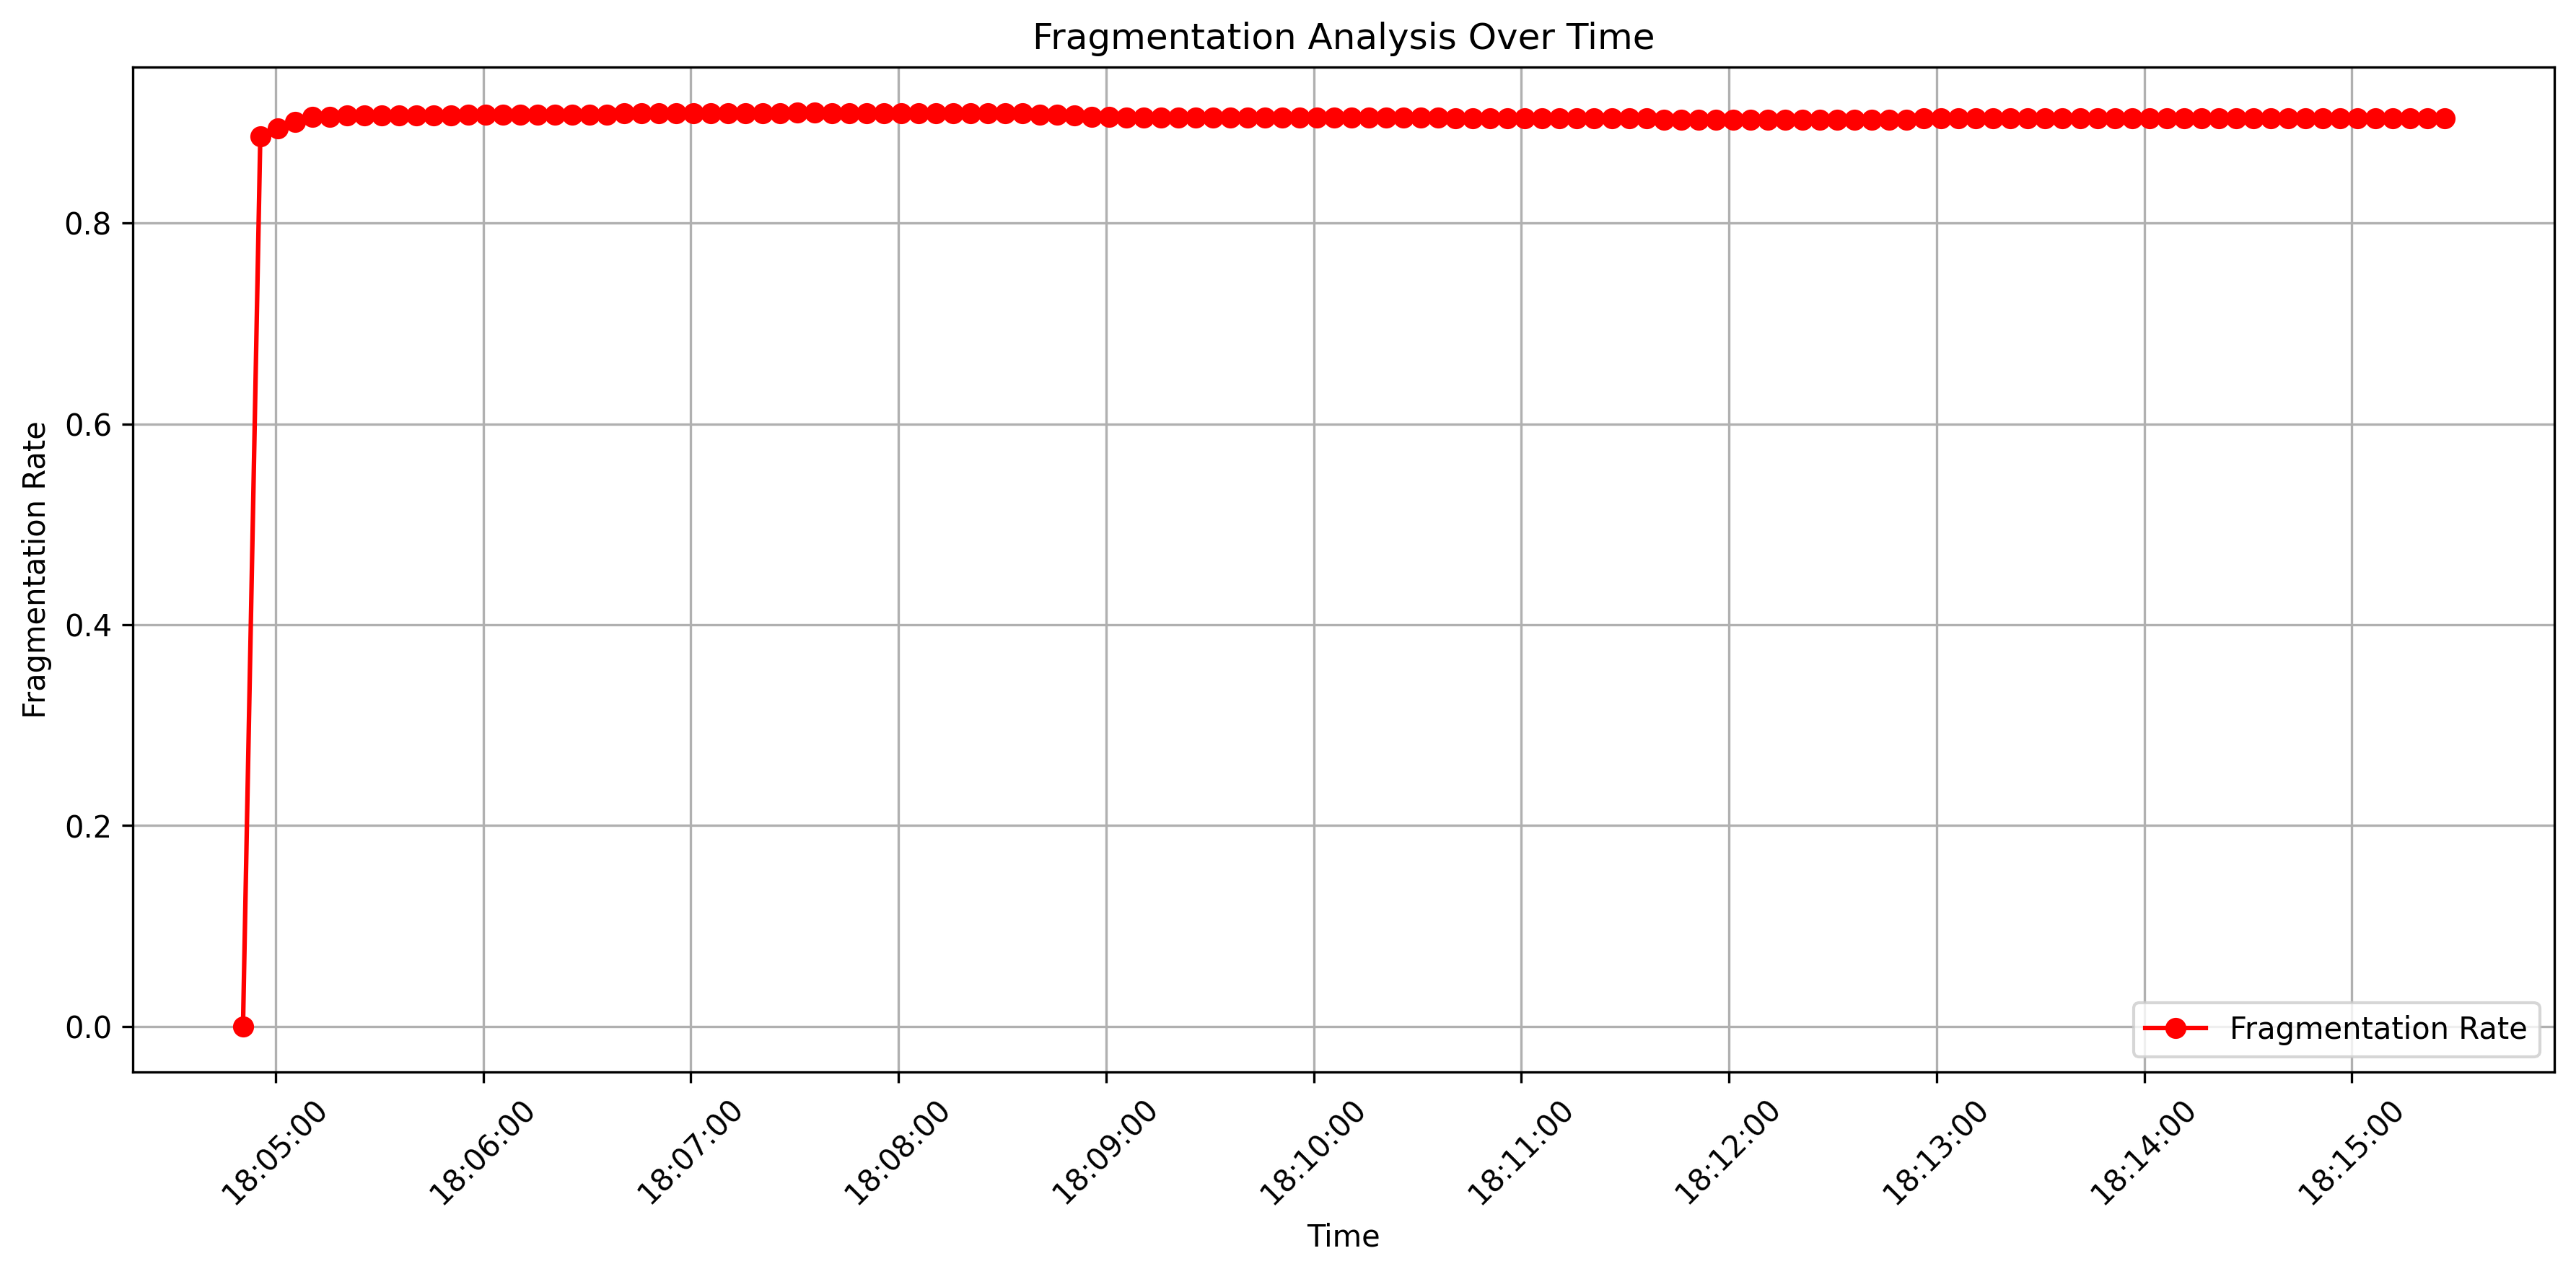
\includegraphics[width=0.8\textwidth]{Evaluation/single_fragmentation_analysis.png}
\caption{Single Client Fragmentation Rate vs Time}
\label{fig:fragmentation-analysis}
\end{figure}

Figure~\ref{fig:fragmentation-analysis} shows the fragmentation behavior throughout the session from 18:05 to 18:15. The fragmentation rate stabilizes at approximately 0.9 (90\%), significantly exceeding the configured threshold of 0.5 (50\%), triggering high fragmentation warnings. Despite this, the system maintained stable performance without degradation in throughput or latency.
The high fragmentation rate is primarily due to the large size of the input data. Media packets, including video streams with substantial frame data and audio packets with buffers of 4096 samples, often exceed the 3000-byte datagram size limit, necessitating fragmentation. These oversized payloads are split across multiple packets, which is expected given the nature of the data streams.



\subsubsection{Throughput Performance}

\begin{figure}[h!]
\centering
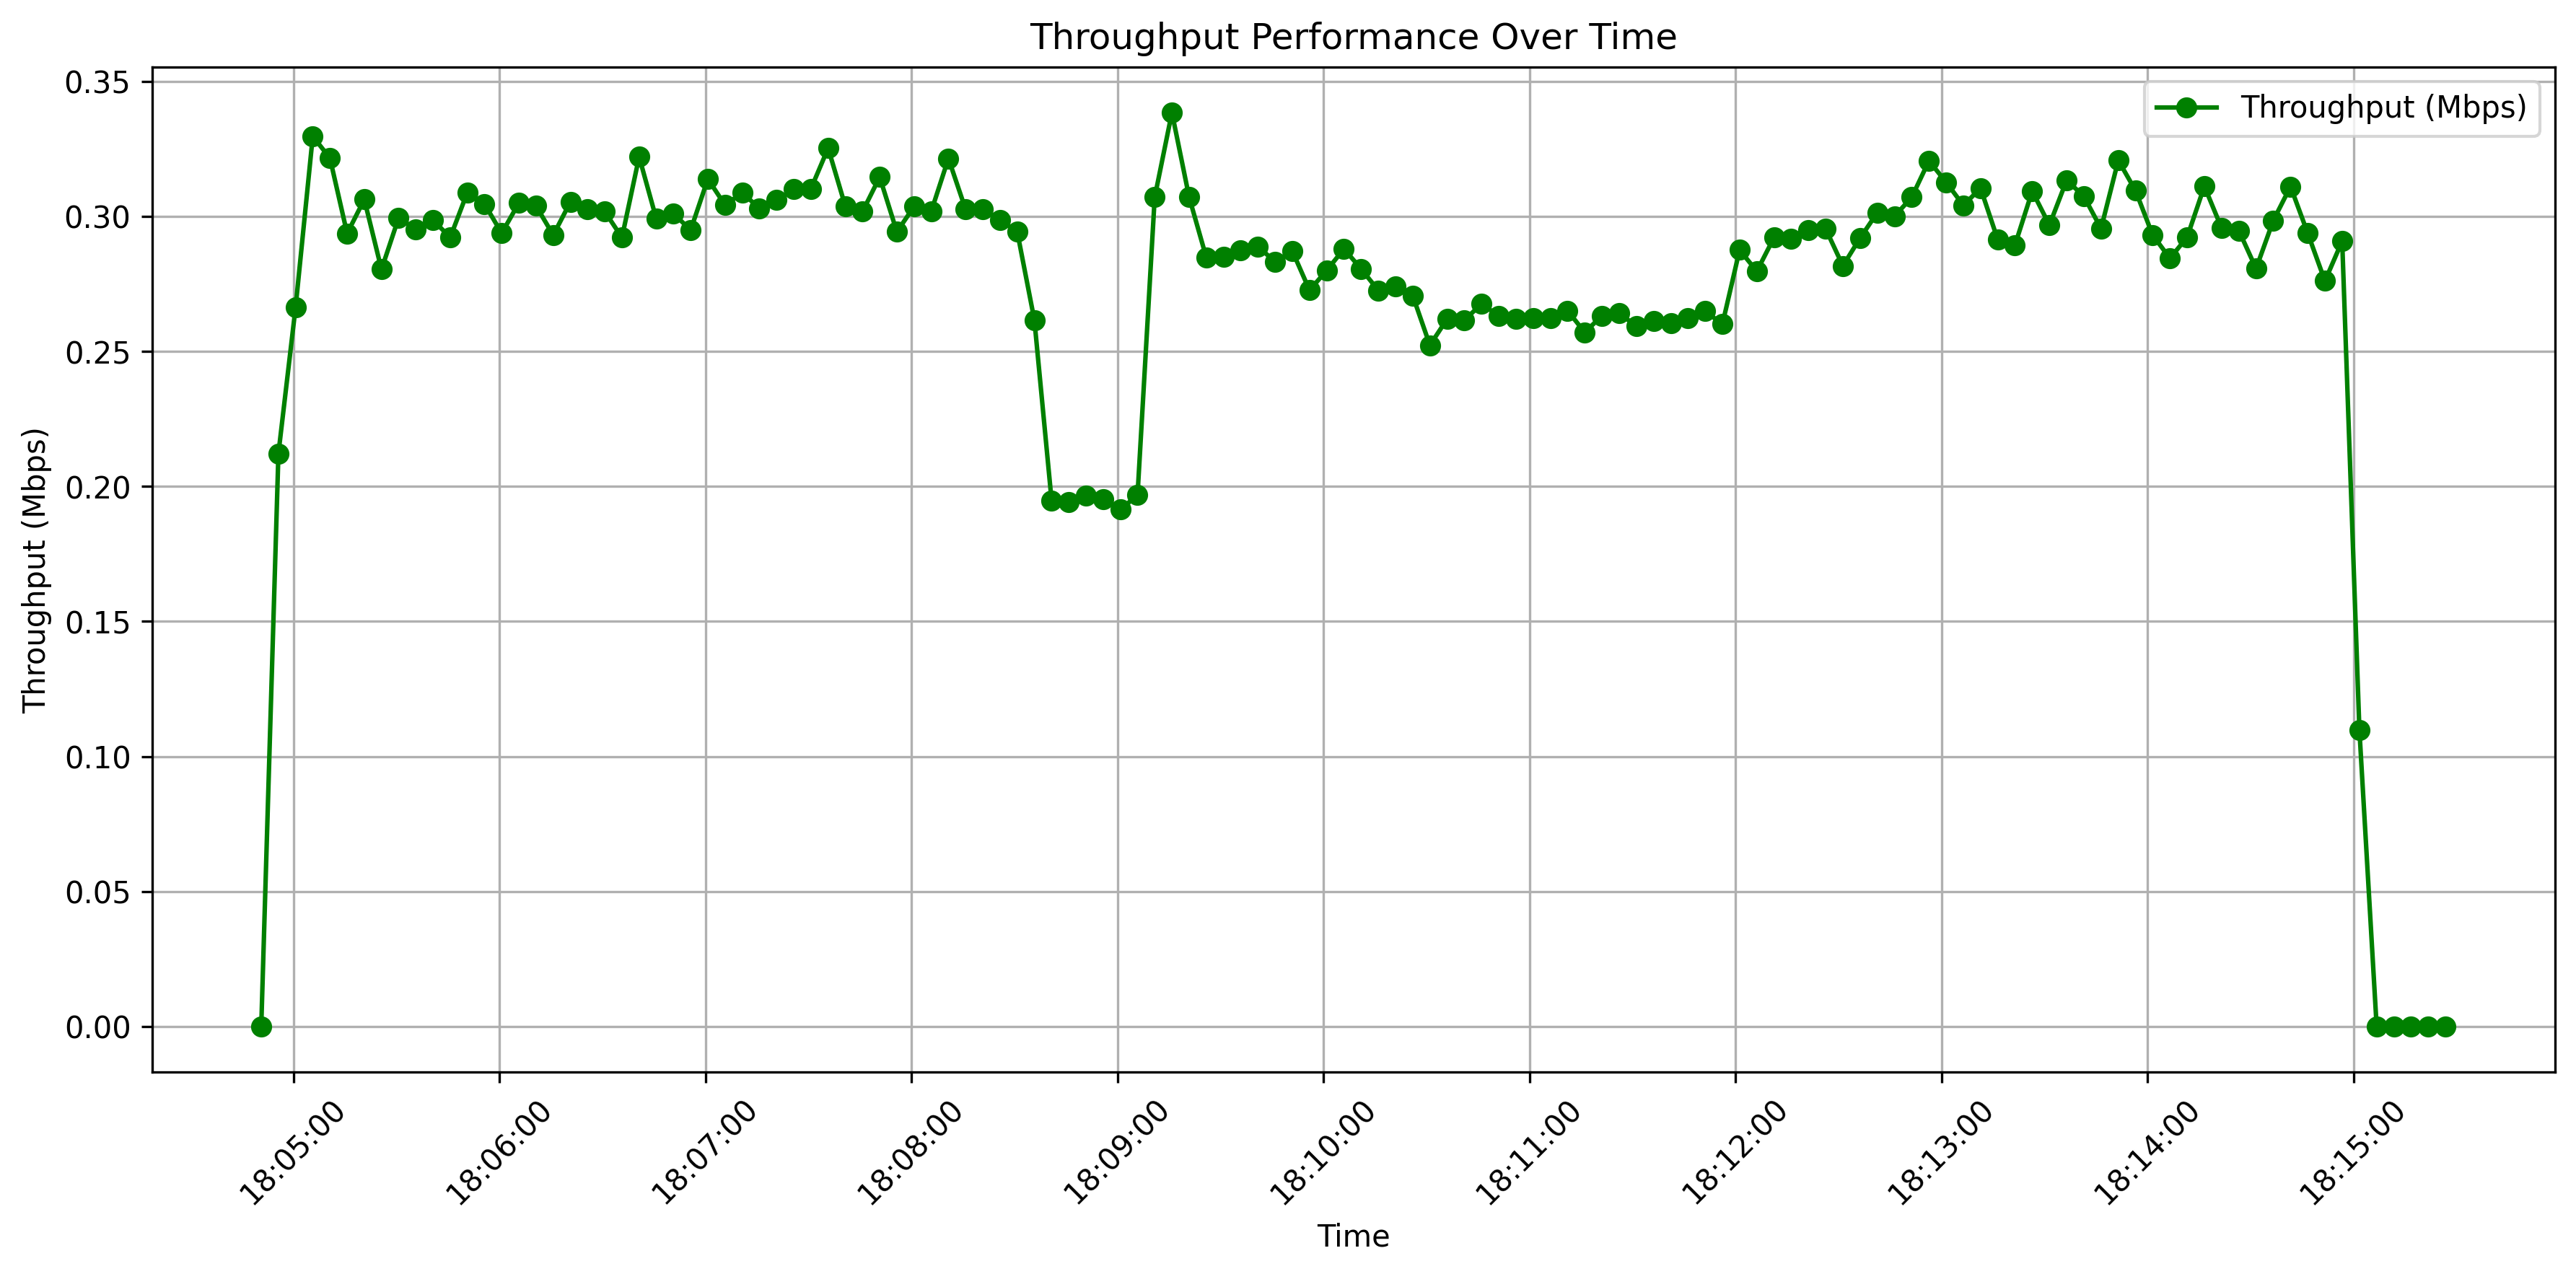
\includegraphics[width=0.8\textwidth]{Evaluation/single_throughput_performance.png}
\caption{Single Client Throughput vs Time}
\label{fig:single-throughput-performance}
\end{figure}

Figure~\ref{fig:single-throughput-performance} displays the throughput performance over time from 18:05 to 18:15. The system maintained a throughput ranging between 0.25 and 0.35 Mbps, with a peak performance of approximately 0.35 Mbps around 18:06-18:07. The throughput declined sharply to 0.0 Mbps at 18:15, corresponding to the session termination.
The throughput analysis indicates an average throughput of about 0.28 Mbps, with variations showing a ±25\% fluctuation from the average. The initial rise to 0.35 Mbps suggests high data handling capacity early in the session, while the dip around 18:08-18:09 reflects a temporary reduction, possibly due to processing adjustments. The smooth decline to 0.0 Mbps at 18:15 indicates a graceful connection termination without abrupt interruptions.


\subsubsection{Latency and Processing Time}
The system exhibited excellent latency performance, with an average processing time of just 0.03-0.04 milliseconds, remaining consistent throughout the session. Similarly, the average buffer wait time was also 0.03-0.04 milliseconds, indicating minimal queuing and efficient data handling. Notably, latency remained stable and showed no observable correlation with fluctuations in throughput or packet fragmentation.

These low latency values confirm the system's suitability for real-time applications requiring minimal processing delays.

\subsubsection{Buffer Management}
Buffer management for (\texttt{client\_134025892847376}), as recorded in the (\texttt{buffer\_metrics\_20250805\_180450.csv}) log between 18:05 and 18:15 on August 5, 2025, demonstrates effective handling of dynamic data loads. The buffer size (\texttt{buffer\_size\_bytes}) varied throughout the session, occasionally dropping to 0 bytes and peaking at 13{,}398 bytes. Initially, the maximum buffer capacity (\texttt{max\_buffer\_size\_bytes}) remained constant at 21{,}475 bytes until 18:08:35, after which it increased to 24{,}281 bytes, indicating an adaptive strategy to accommodate increased data traffic. Notably, no buffer overflows (\texttt{buffer\_overflows}) were recorded, reflecting the system’s robust buffer allocation and the ability to absorb traffic fluctuations without packet loss.

\subsection{Three-Client Performance Analysis}
The three-client experiment characterizes the WebTransport router under a moderate, multi-tenant load.
\begin{figure}[h!]
\centering
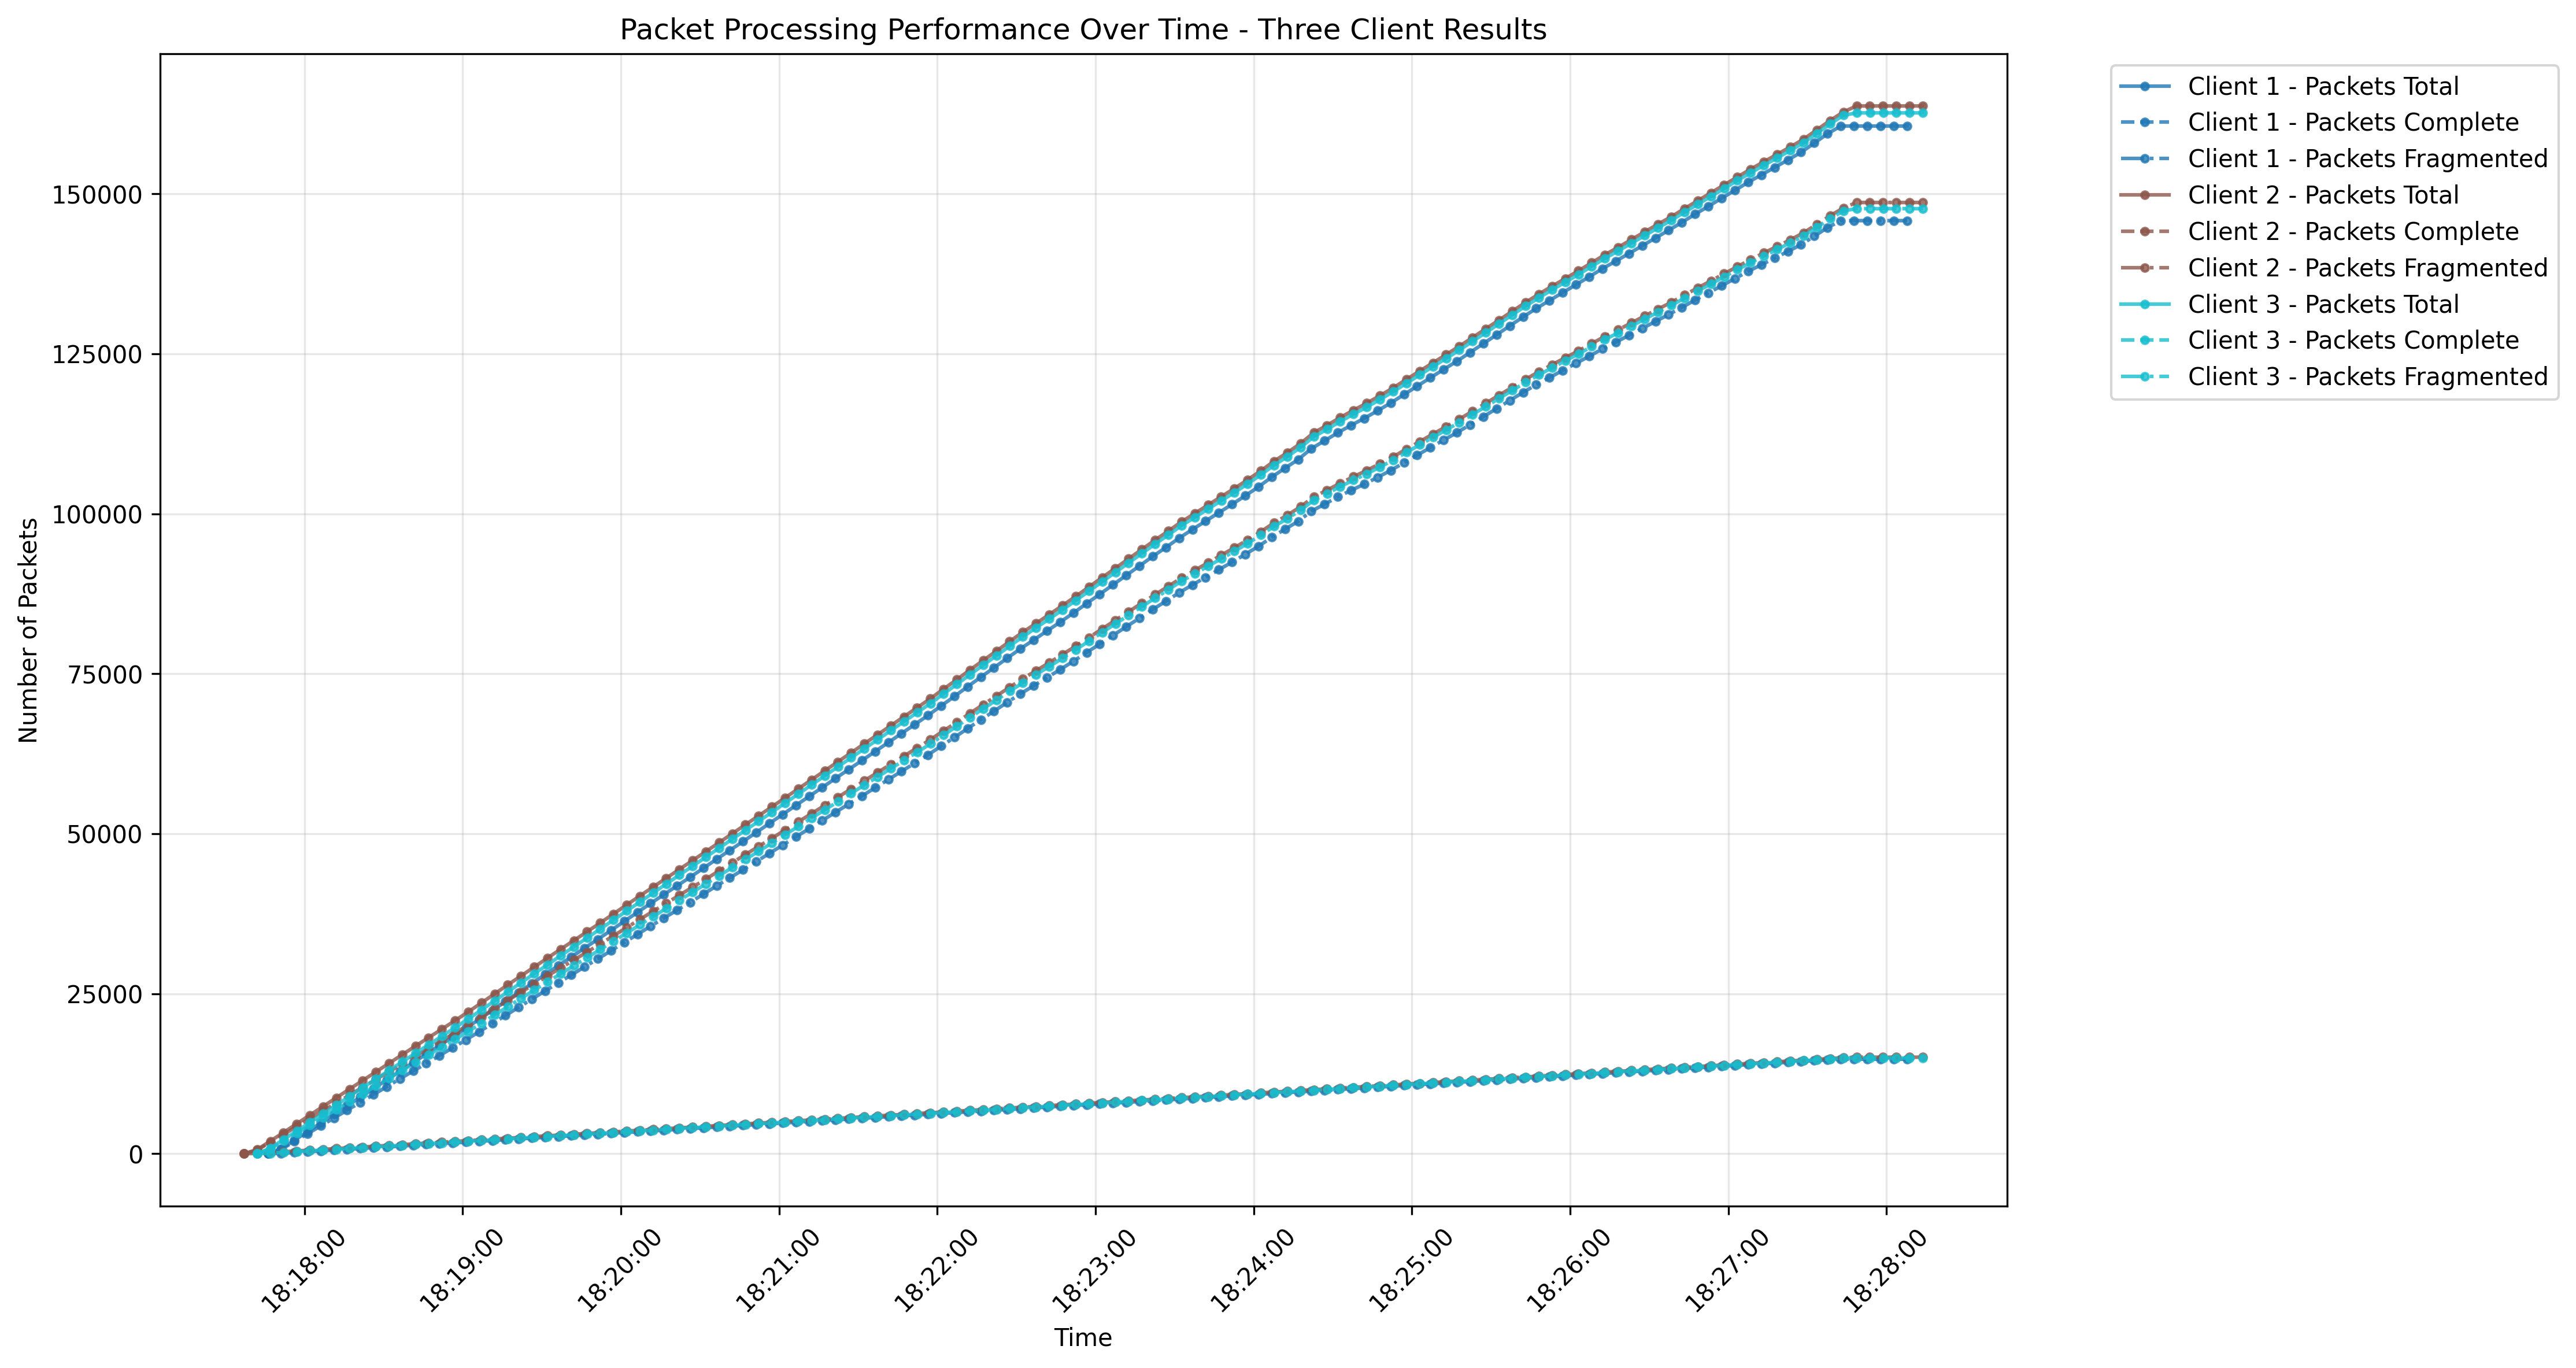
\includegraphics[width=0.8\textwidth]{Evaluation/packet_processing_by_client_three-client-results.png}
\caption{Packet Processing Performance Over Time – Three Client Results}
\label{fig:packet-processing-three-clients}
\end{figure}
Figure~\ref{fig:packet-processing-three-clients} illustrates the packet processing performance across three clients from 18:05 to 18:15, with the router handling approximately 487,000 packets in total. Each client processed: Client 1 with 160,586 packets, Client 2 with 162,643 packets, and Client 3 with 163,724 packets. The per-second arrival rate was linear and nearly identical across clients, indicating fair scheduling. Fragmentation averaged 90.8\%, resulting in about 442,000 fragmented packets and 45,000 complete packets, with a 100\% successful reassembly rate and no logged losses.\

\subsubsection{Three Client Fragmentation Analysis}
\begin{figure}[h!]
\centering
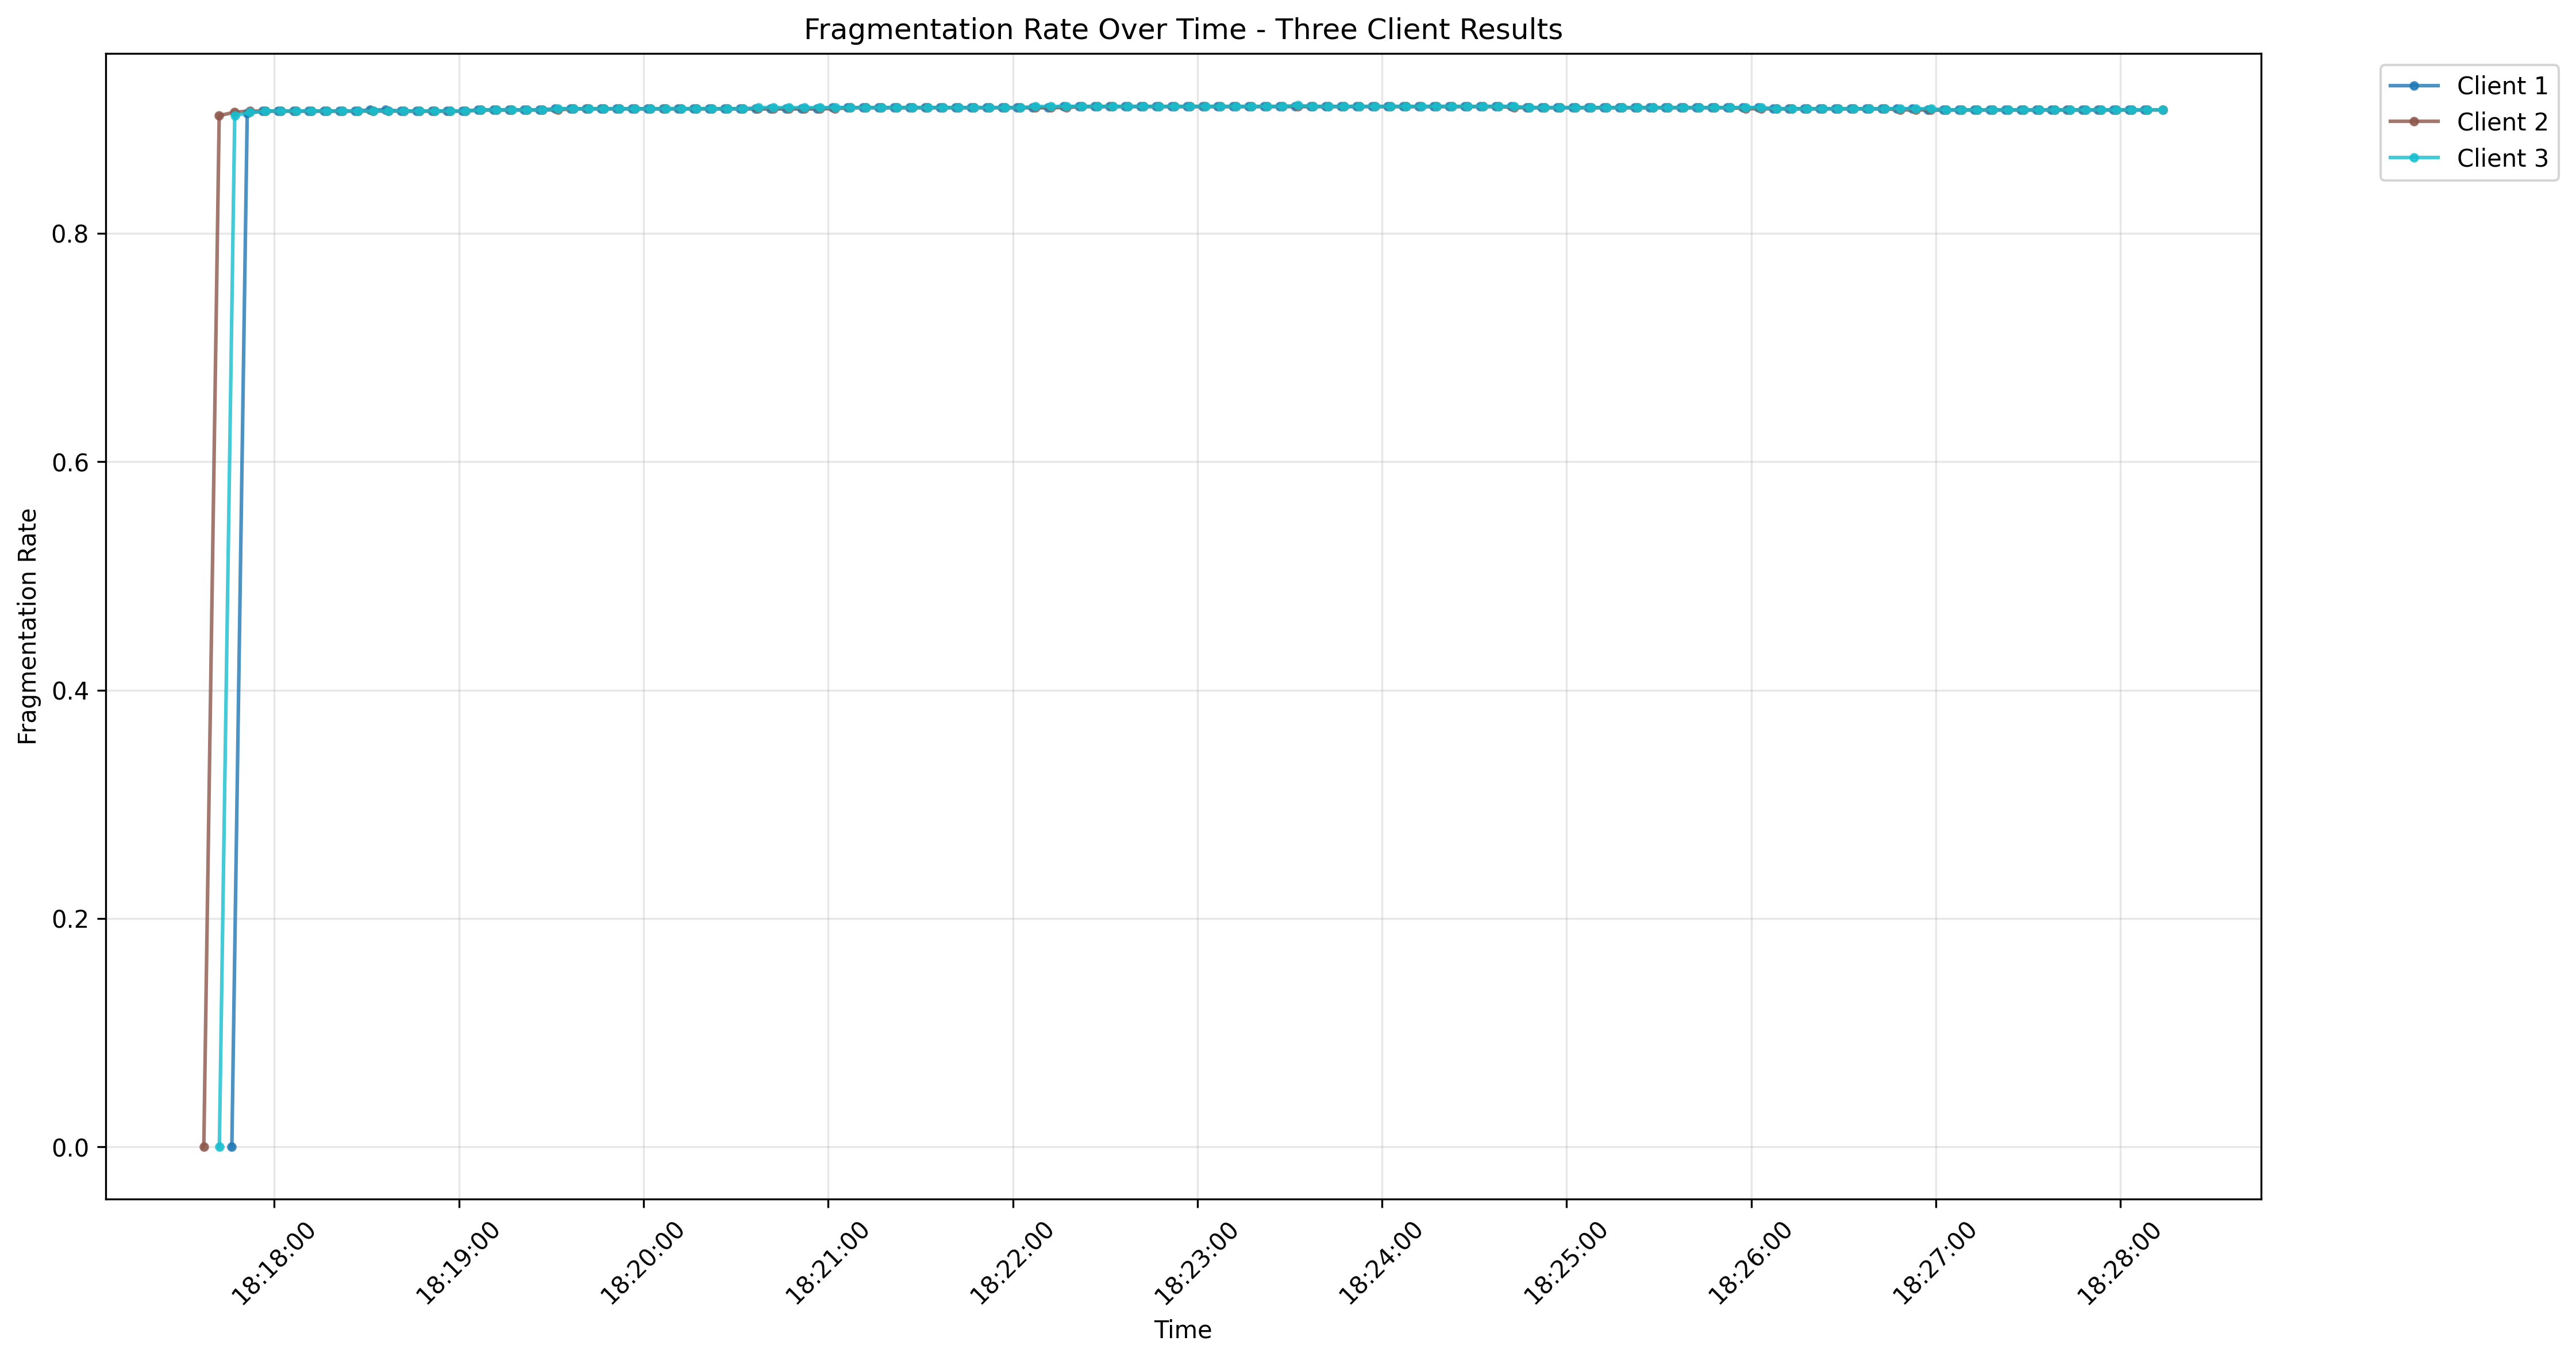
\includegraphics[width=0.8\textwidth]{Evaluation/fragmentation_by_client_three-client-results.png}
\caption{Fragmentation Rate Over Time – Three Client Results}
\label{fig:fragmentation-three-clients}
\end{figure}
Figure~\ref{fig:fragmentation-three-clients} shows the fragmentation behavior across the three clients, stabilizing at 0.9–0.91 (90–91\%), consistently exceeding the 0.5 (50\%) threshold and triggering high fragmentation warnings. The high rate is attributed to 4,096-sample audio buffers and large video frames surpassing the 3,000-byte datagram limit. Despite uniform 90\% fragmentation, throughput and latency remained stable, suggesting linear scalability in the fragmentation/reassembly path.


\subsubsection{Three Client Throughput Analysis}
\begin{figure}[h!]
\centering
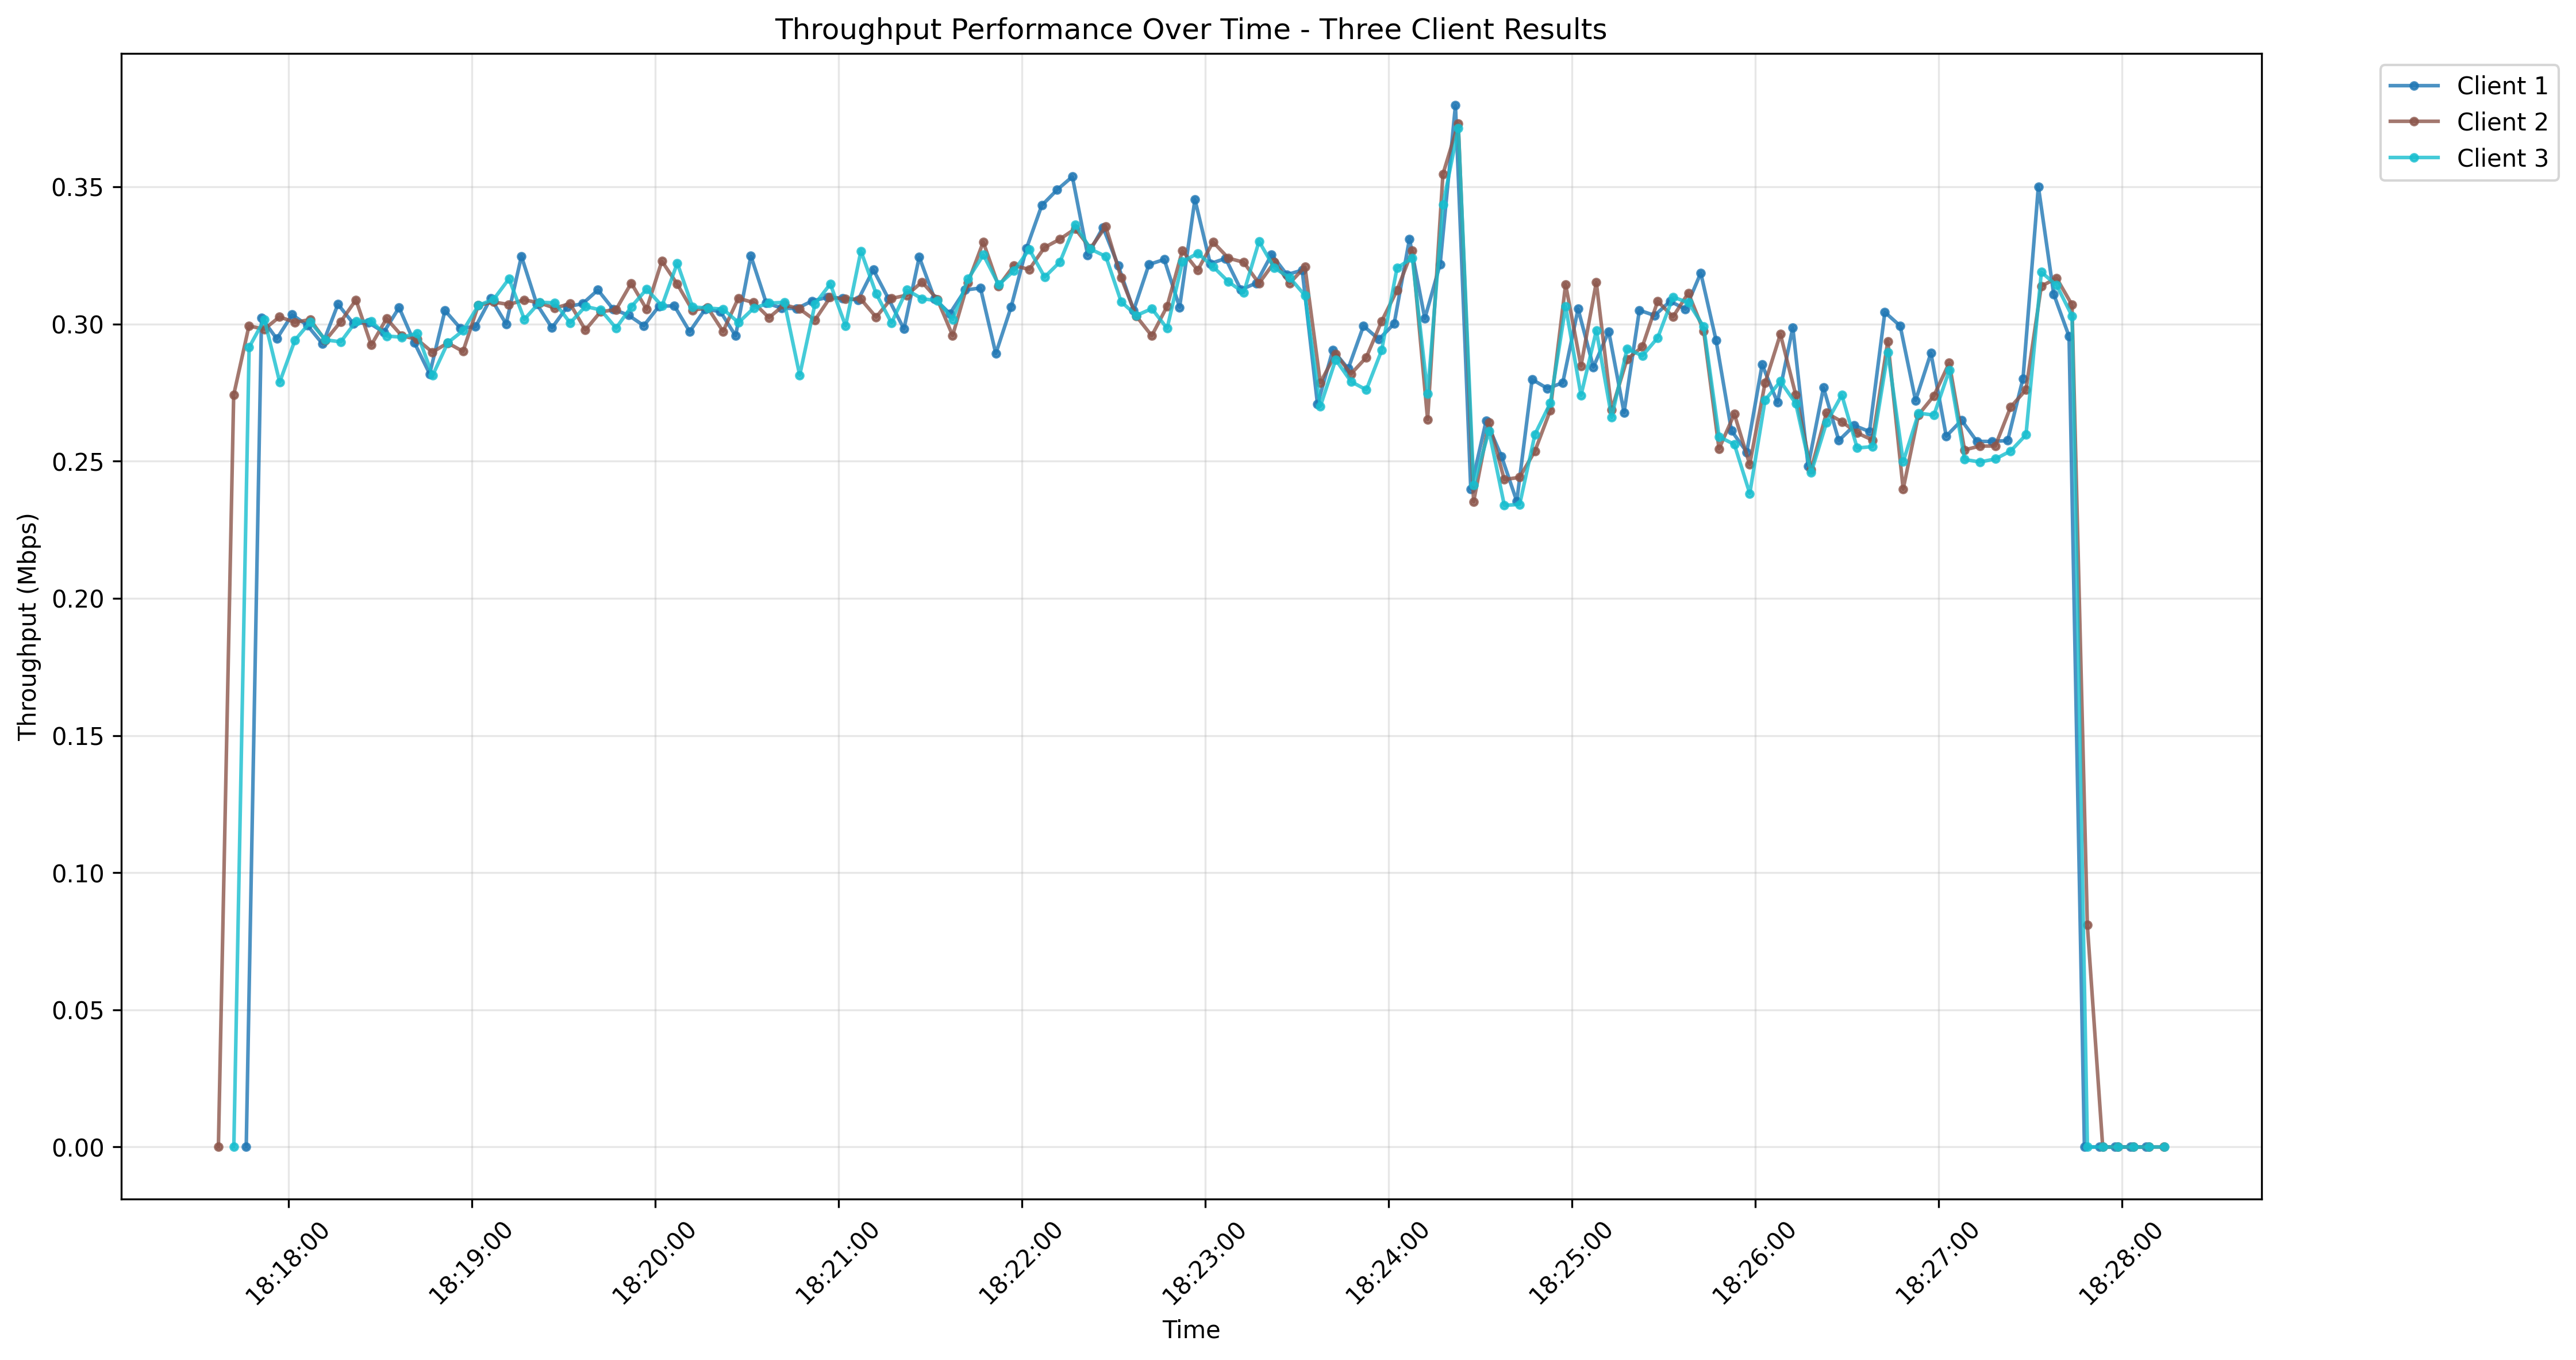
\includegraphics[width=0.8\textwidth]{Evaluation/throughput_by_client_three-client-results.png}
\caption{Throughput Over Time – Three Client Results}
\label{fig:throughput-three-clients}
\end{figure}
Figure~\ref{fig:throughput-three-clients} displays the throughput performance per client, with an average of 0.30 Mbps, an aggregate average of 0.90 Mbps, a peak of 0.38 Mbps, and a minimum of 0.23 Mbps. Throughput curves were smooth and uncorrelated, ruling out head-of-line blocking, with a brief dip to 0 Mbps at the end marking graceful connection teardown.

\begin{figure}[h!]
\centering
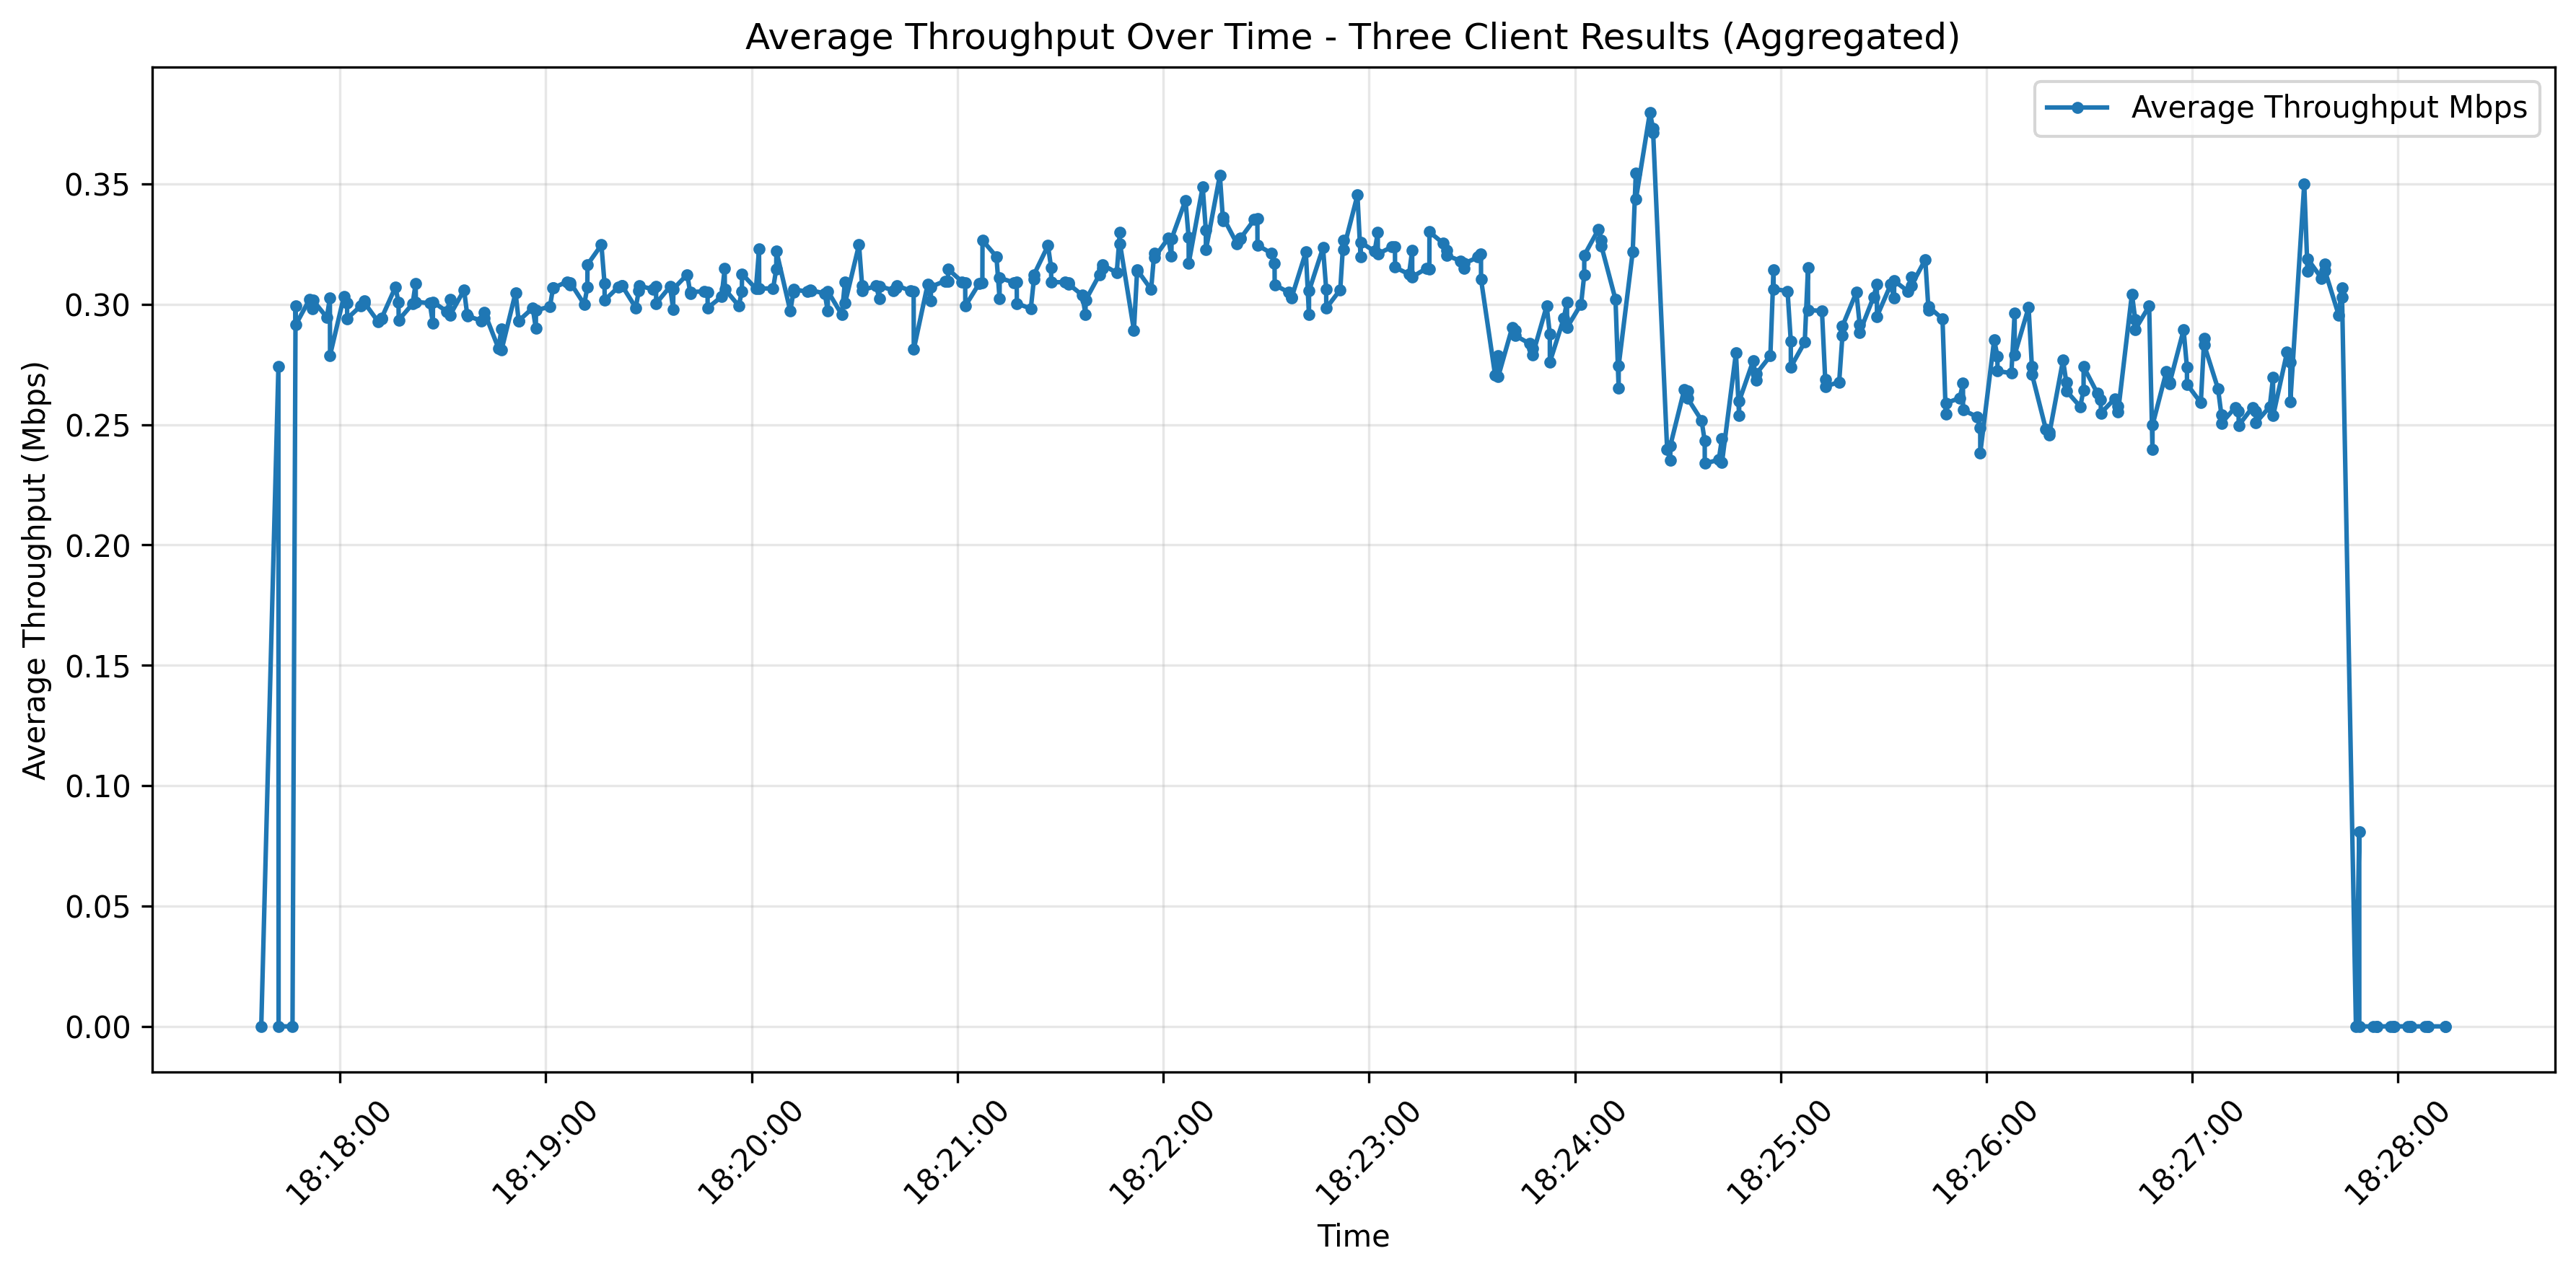
\includegraphics[width=0.8\textwidth]{Evaluation/avg_throughput_aggregated_three-client-results.png}
\caption{Average Aggregated Throughput}
\label{fig:avg-throughput-aggregated}
\end{figure}
Figure~\ref{fig:avg-throughput-aggregated} shows the combined throughput maintaining a steady 0.85–0.90 Mbps plateau, with no multi-second zero-throughput periods until deliberate shutdown.

\subsubsection{Router Pod Overview}
The router pod utilized 418 m (≈ 0.42 core) of CPU and 92 MiB of memory, with no restarts and stable performance throughout the 11-minute window, indicating modest control-plane and data-plane overhead for handling three clients.
\begin{figure}[h!]
\centering
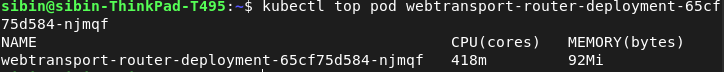
\includegraphics[width=0.8\textwidth]{Evaluation/three-clients-stats.png}
\caption{Router Pod Performance for 3 clients}
\label{fig:three-clients-stats}
\end{figure}

\subsubsection{Host Machine Overview}
The host machine showed CPU usage between 29.9\% and 40.6\% across cores (averaging around 35\%), memory usage at 8.53 GiB / 13.5 GiB (63\%), and a load of 2.85 / 2.16 / 2.04 with 308 tasks (2 running). Utilization was healthy with no swap thrashing, confirming ample headroom.

\begin{figure}[h!]
\centering
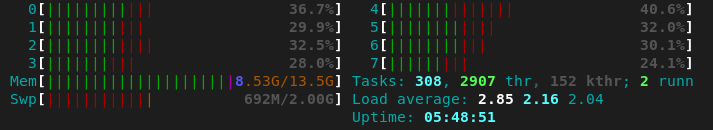
\includegraphics[width=0.8\textwidth]{Evaluation/three-clients-host-stats.png}
\caption{Host Machine stats for 3 clients}
\label{fig:three-clients-host-stats}
\end{figure}

\subsubsection{Latency and Processing Time}
Latency remained sub-millisecond, with an average processing time of 0.02–0.04 ms and an average buffer wait time of 0.02–0.04 ms across all clients, indicating no increase in per-packet overhead with additional concurrent clients.
\subsubsection{Buffer Management}
Each client maintained an independent buffer ring, with the maximum buffer size auto-tuning from 16–17 kB to 24 kB as traffic increased. Peak usage reached 18,270 bytes (Client 1), well below the 24 kB limit, and no buffer overflows were recorded, demonstrating effective back-pressure and kernel socket buffer management


\subsection{Five-Client Performance Analysis}
The five-client experiment extends the scaling study to 15 concurrent media streams (5 clients × 3 streams each) and represents the first high-load scenario for the WebTransport router.
\begin{figure}[h!]
\centering
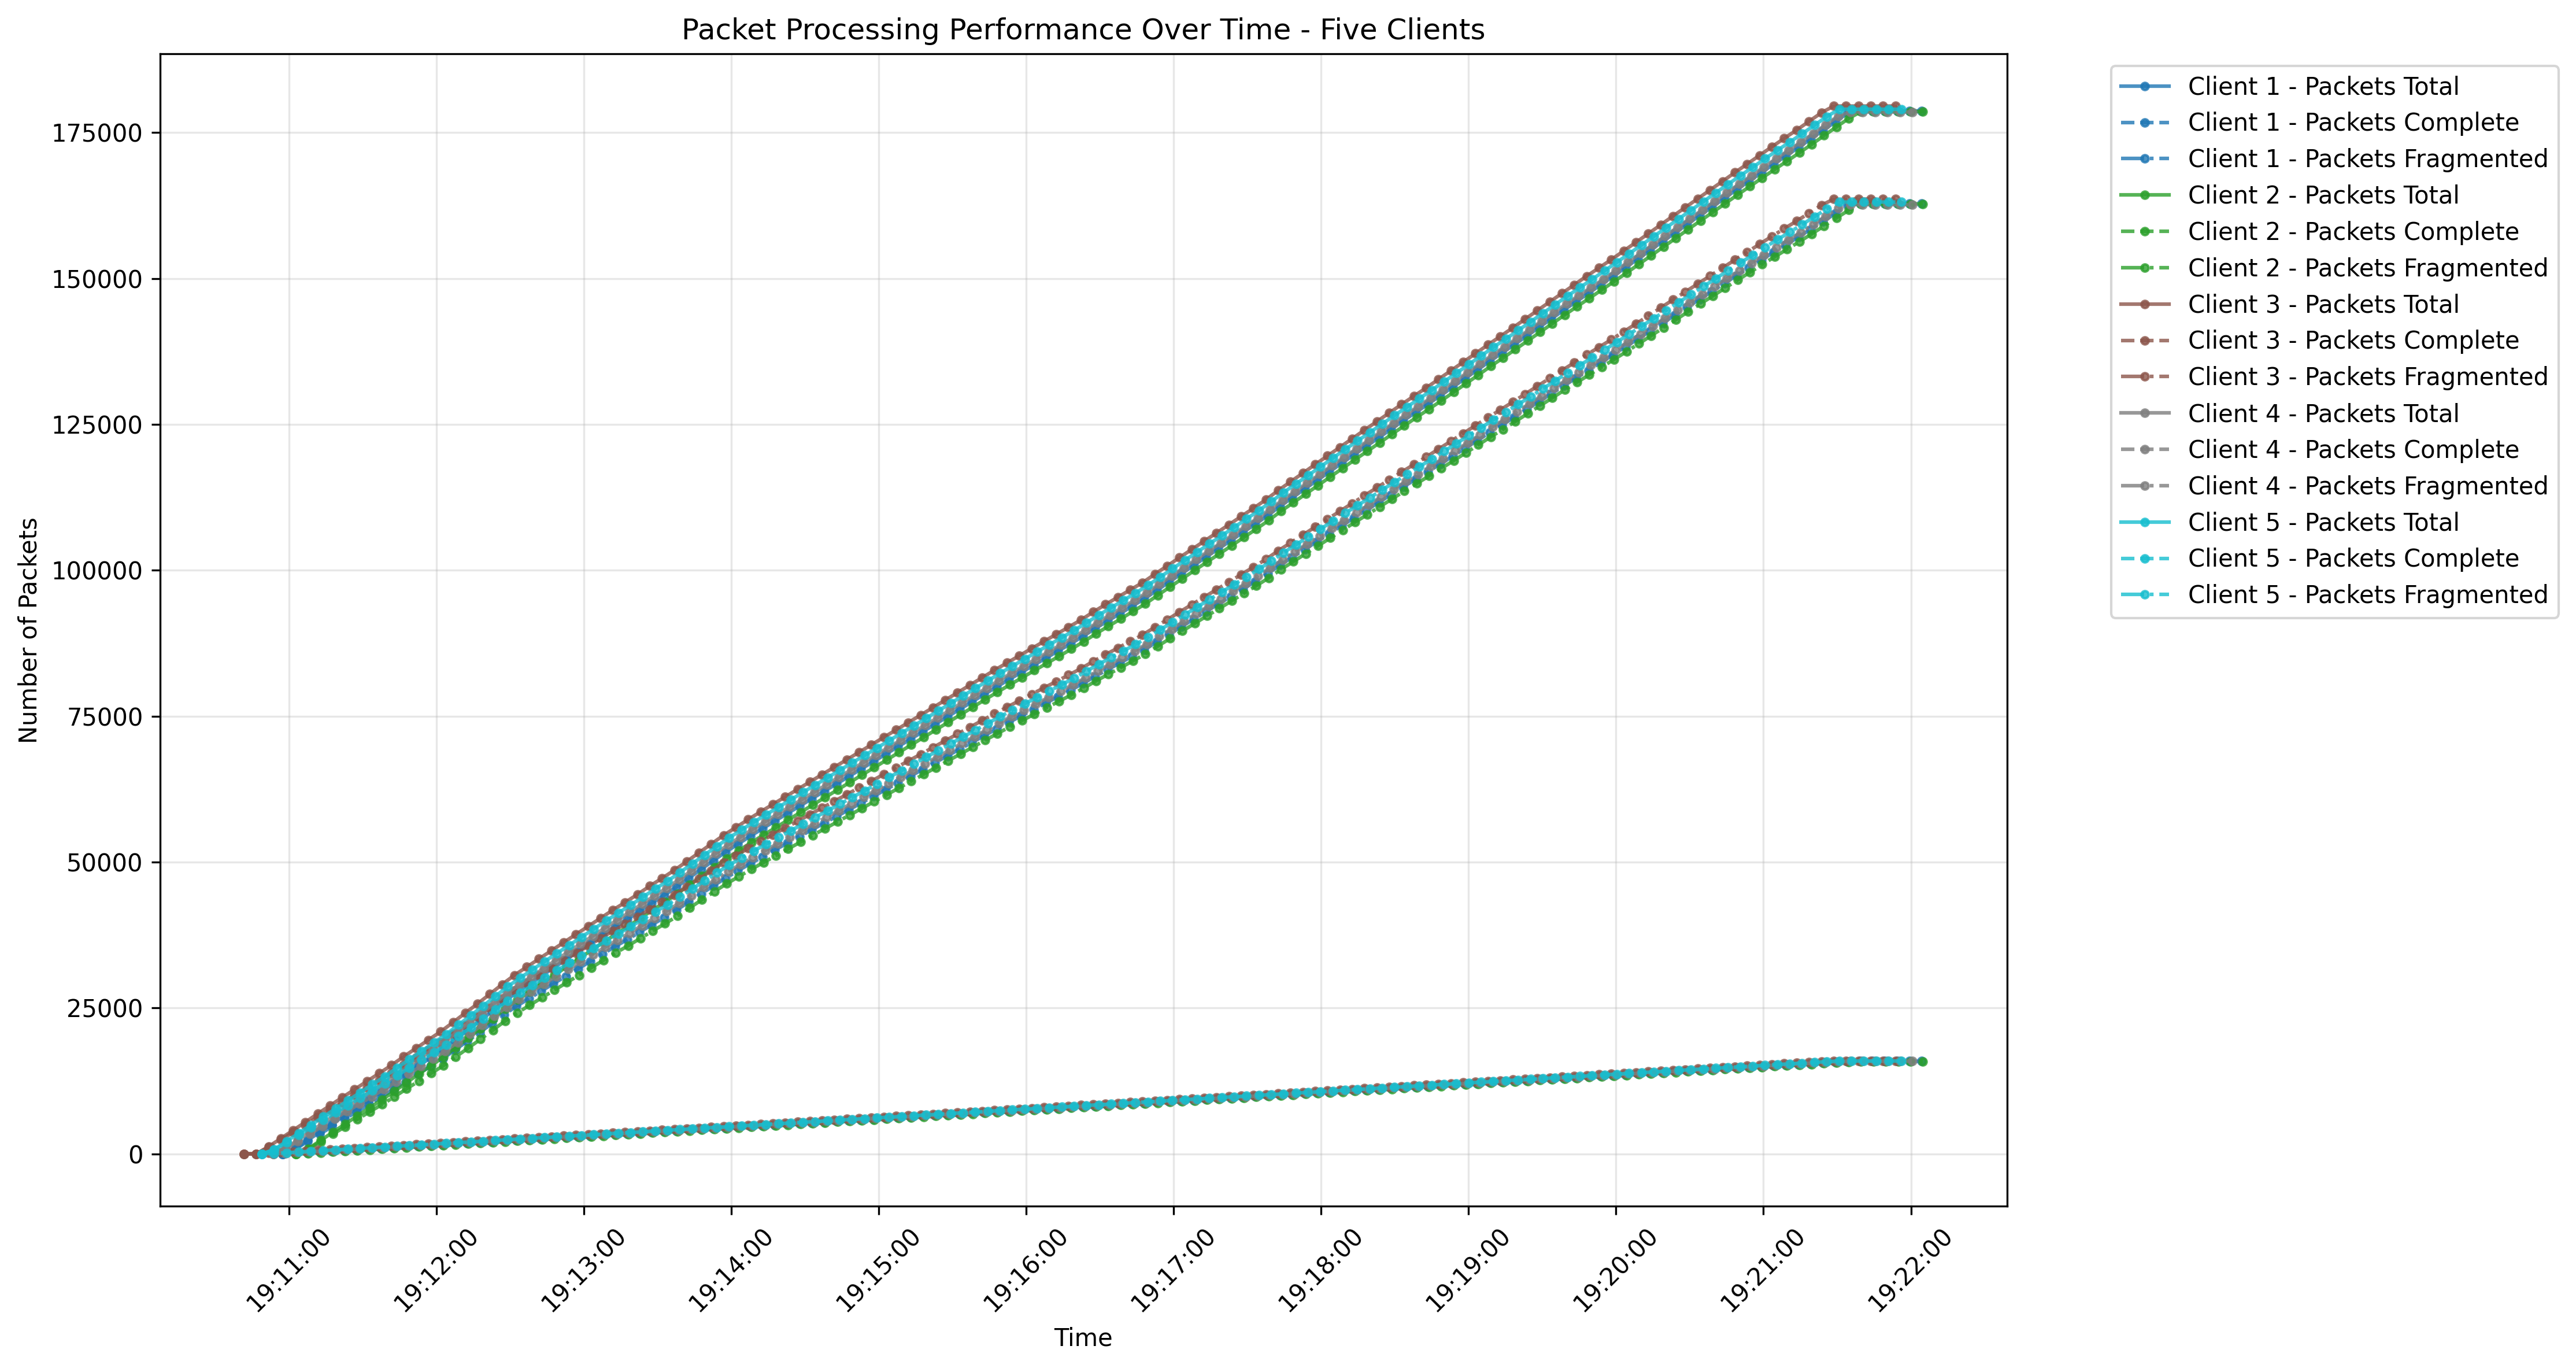
\includegraphics[width=0.8\textwidth]{Evaluation/packet_processing_by_client_five-clients.png}
\caption{Packet Processing – Five Clients}
\label{fig:packet-processing-five-clients}
\end{figure}
Figure~\ref{fig:packet-processing-five-clients} illustrates the packet processing performance across five clients from 19:10 to 19:22 on August 5, 2025, with an aggregate of approximately 890,000 packets. Per-client packet counts ranged from 175,000 to 180,000, showing linear growth and fair scheduling without head-of-line blocking. The fragmentation rate varied between 90.8\% and 91.6\%, with 100\% reassembly success and no packet losses.
\begin{figure}[h!]
\centering
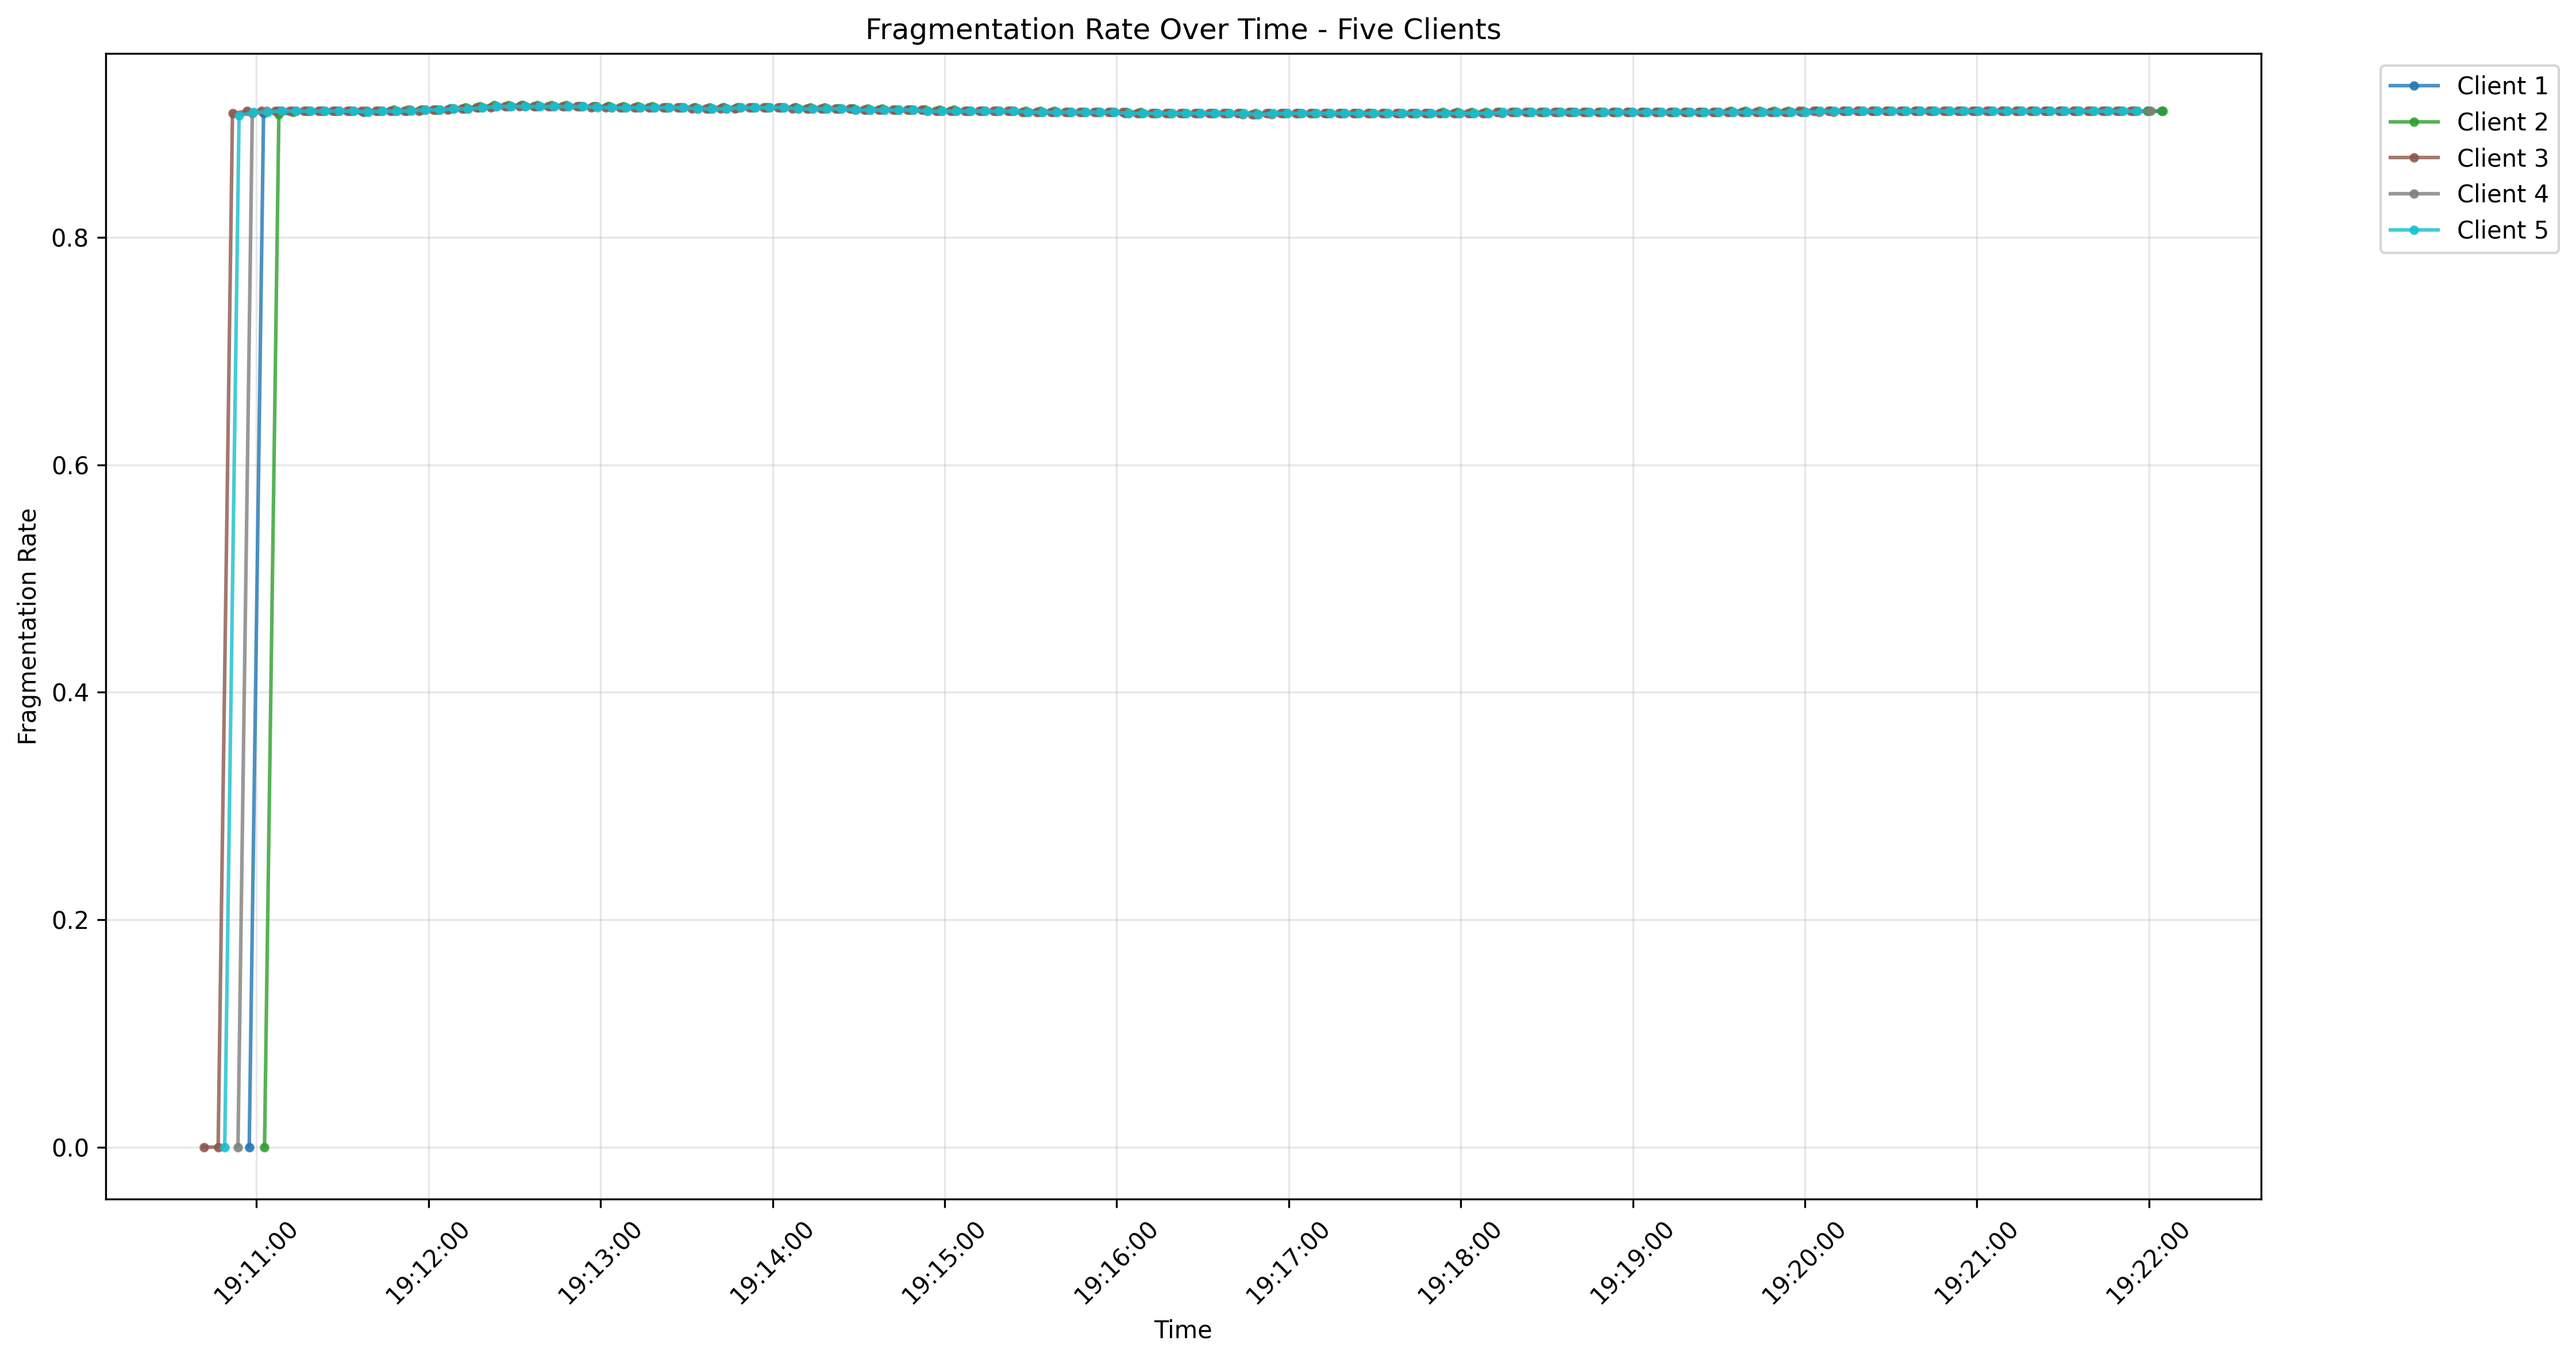
\includegraphics[width=0.8\textwidth]{Evaluation/fragmentation_by_client_five-clients.png}
\caption{Fragmentation Rate – Five Clients}
\label{fig:fragmentation-five-clients}
\end{figure}
Figure~\ref{fig:fragmentation-five-clients} displays the fragmentation behavior across the five clients, stabilizing at approximately 0.9 (90\%), consistently triggering HIGH\_FRAGMENTATION warnings. The high rate is due to 4,096-sample audio buffers and large video frames exceeding the 3,000-byte datagram limit, yet throughput and latency remained unaffected, highlighting efficient reassembly.
\begin{figure}[h!]
\centering
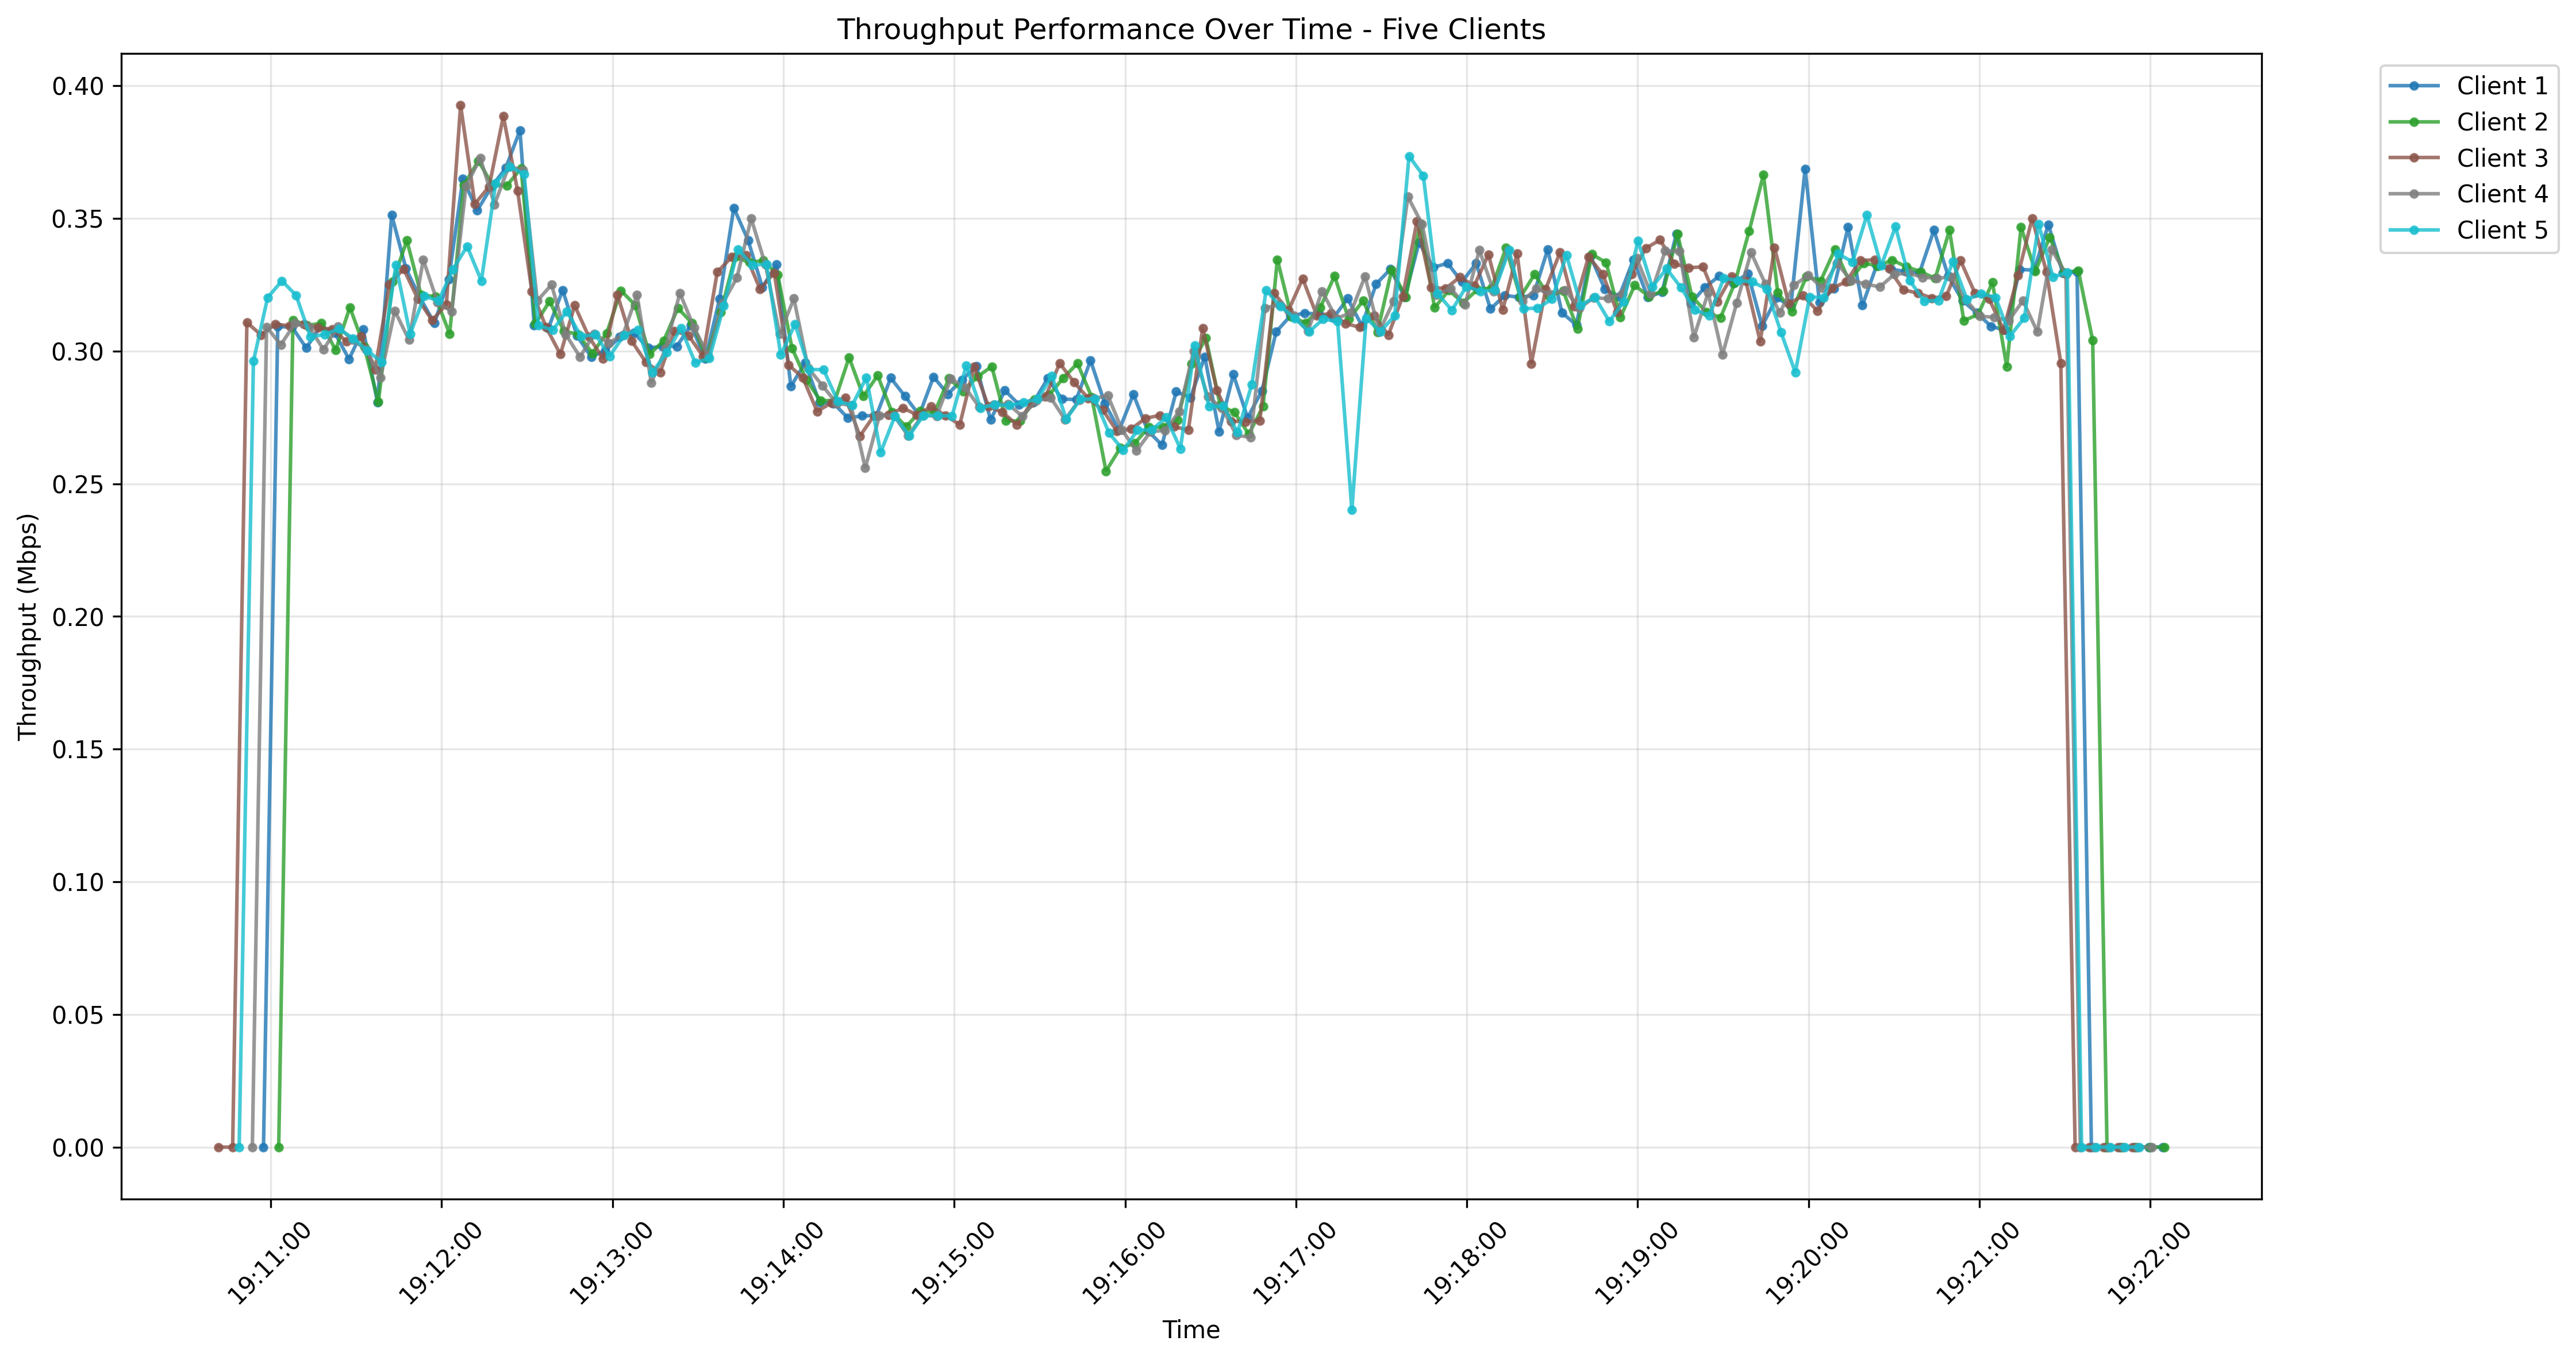
\includegraphics[width=0.8\textwidth]{Evaluation/throughput_by_client_five-clients.png}
\caption{Throughput – Five Clients}
\label{fig:throughput-five-clients}
\end{figure}
Figure~\ref{fig:throughput-five-clients} shows the throughput performance per client, with an average of 0.315 Mbps, an aggregate average of 1.58 Mbps, a peak of 0.395 Mbps, and a lowest trough of 0.23 Mbps. The aggregate trace was smooth, with no multi-second drops until deliberate shutdown.
\begin{figure}[h!]
\centering
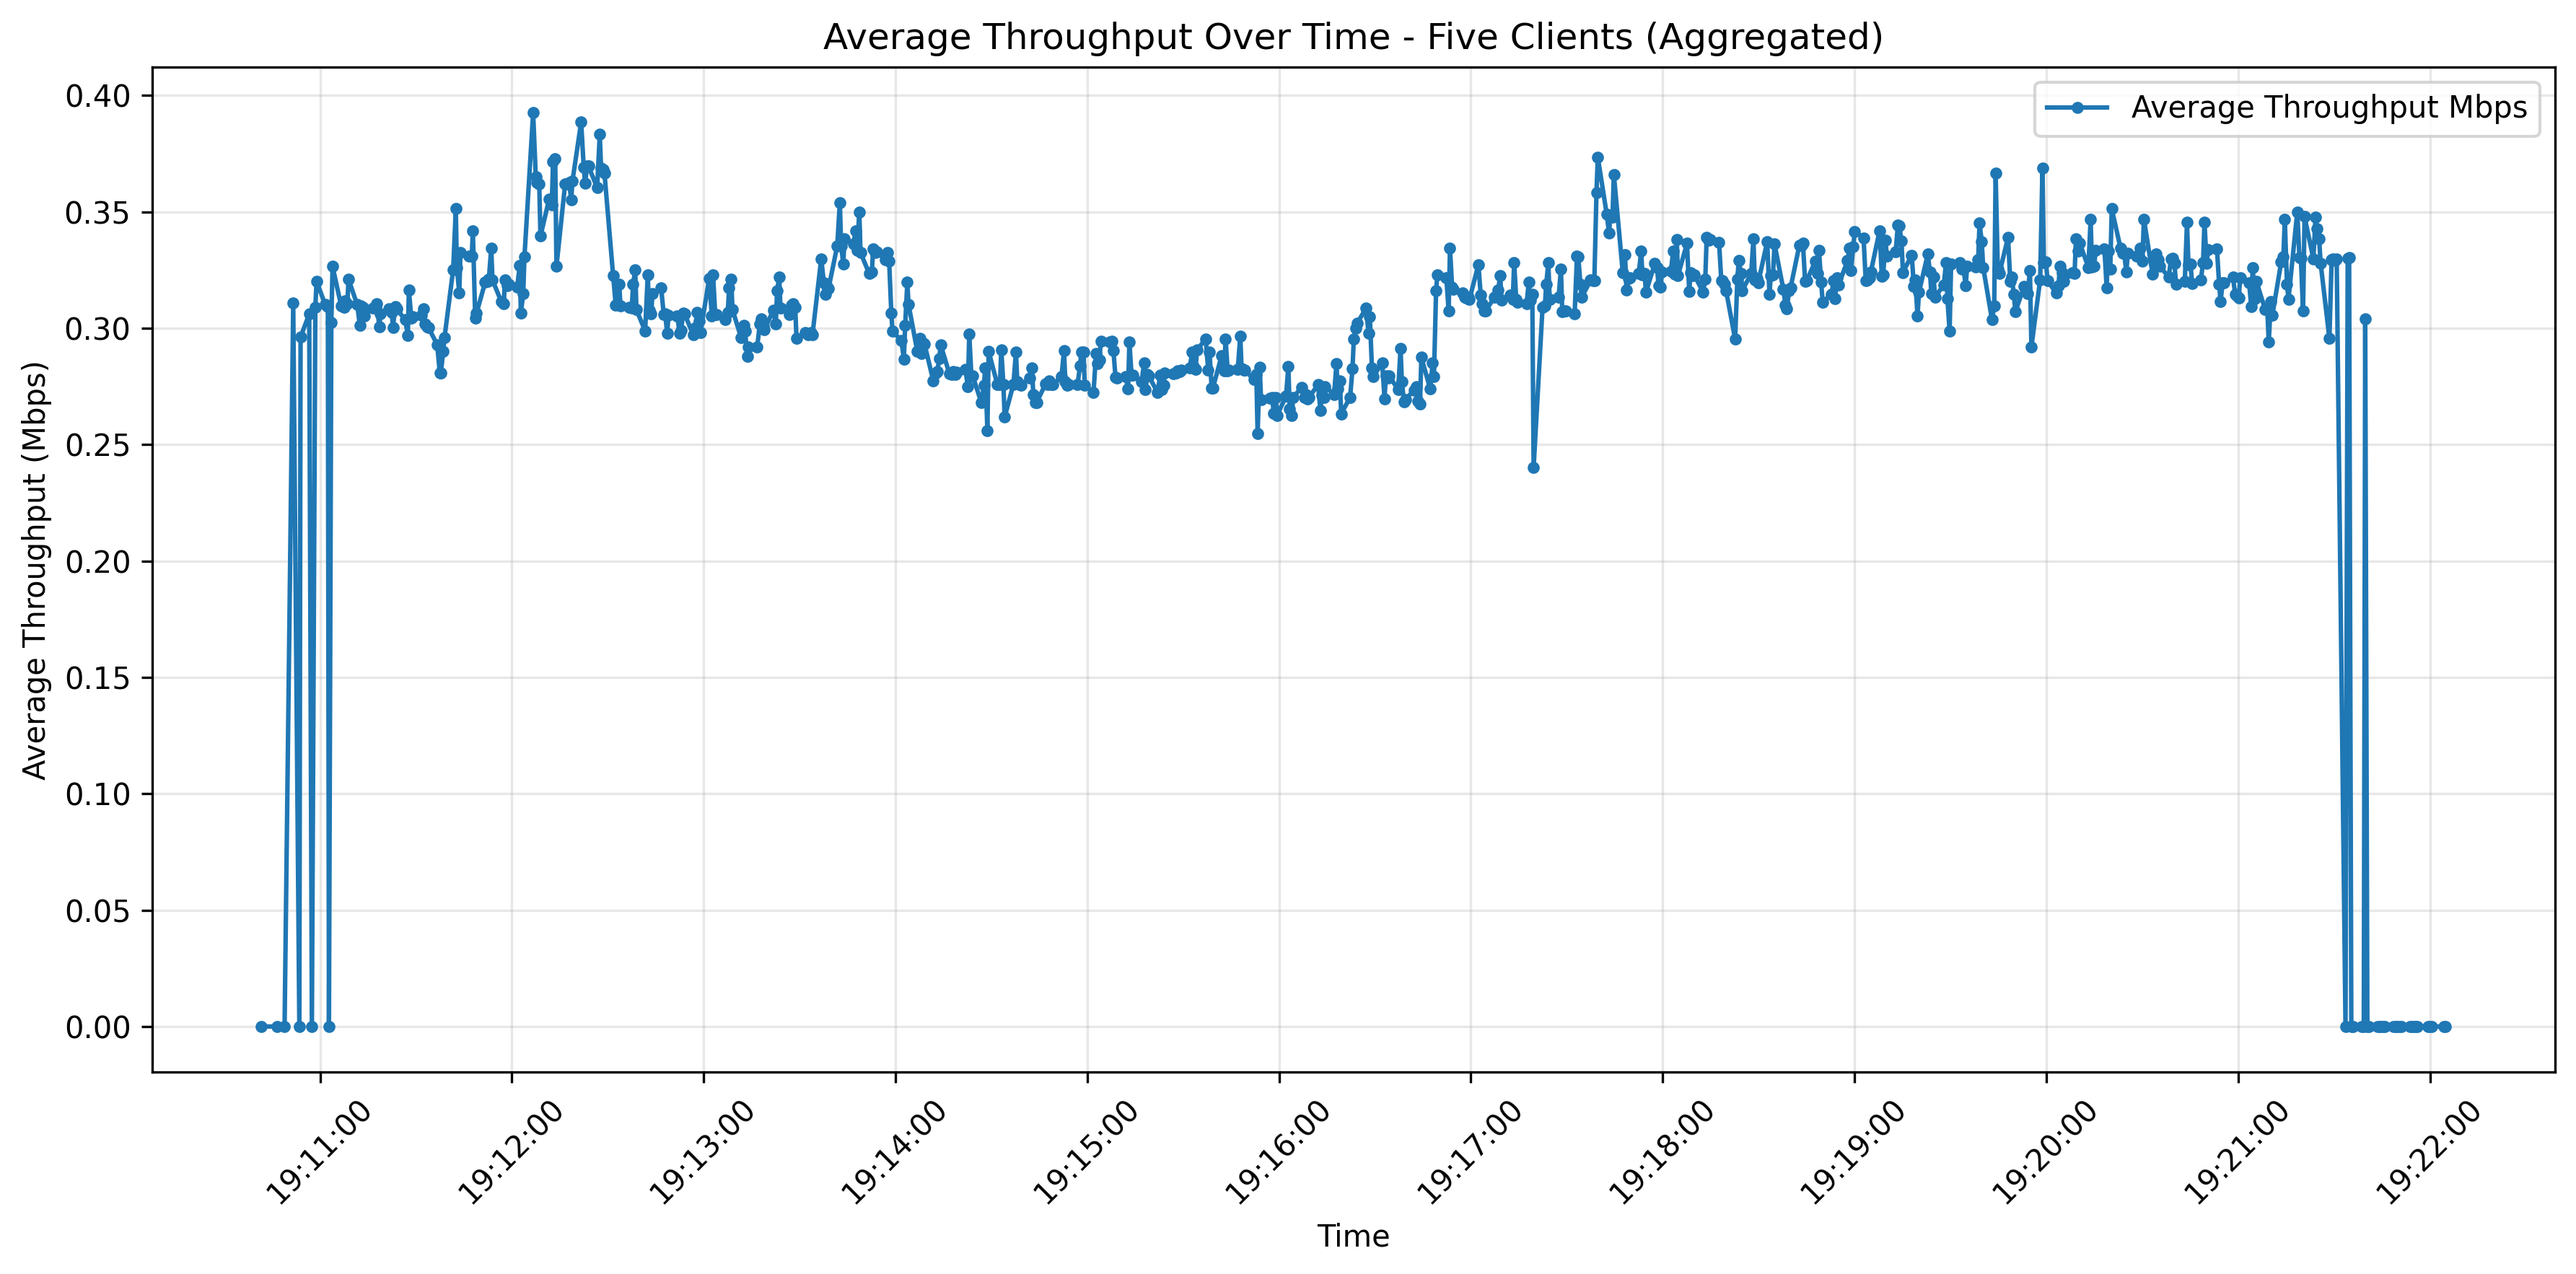
\includegraphics[width=0.8\textwidth]{Evaluation/avg_throughput_aggregated_five-clients.png}
\caption{Aggregated Throughput – Five Clients}
\label{fig:avg-throughput-aggregated-five}
\end{figure}
Figure~\ref{fig:avg-throughput-aggregated-five} presents the combined throughput oscillating between 1.5–1.6 Mbps for most of the run, validating near-linear scaling from the three-client baseline.

\subsubsection{Router Pod Overview}
\begin{figure}[h!]
\centering
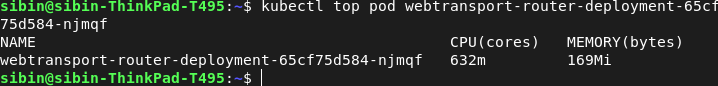
\includegraphics[width=0.8\textwidth]{Evaluation/five-clients-pod-stats.png}
\caption{Router Pod Performance – Five Clients}
\label{fig:router-pod-five-clients}
\end{figure}

Figure~\ref{fig:router-pod-five-clients} shows the router pod performance at 10:54 PM BST on August 5, 2025, utilizing approximately 0.42 core (418 m) of CPU and 92 MiB of memory, with no restarts and stable uptime for 12 minutes. CPU utilisation remained unchanged compared to the three-client run, indicating sub-linear control-plane overhead scaling with client count.

\subsubsection{Host Machine Overview}
\begin{figure}[h!]
\centering
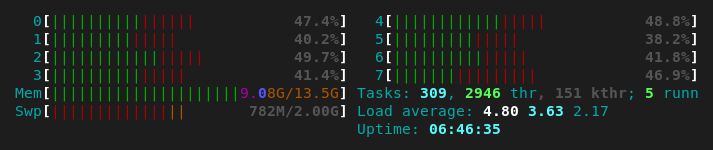
\includegraphics[width=0.8\textwidth]{Evaluation/five-clients-machine-stats.png}
\caption{Host Machine Performance – Five Clients}
\label{fig:host-machine-five-clients}
\end{figure}

Figure~\ref{fig:host-machine-five-clients} depicts the host machine performance at 10:54 PM BST on August 5, 2025, peaking at 40.6\% CPU usage across cores, using 8.53 GiB / 13.5 GiB (63\%) memory, maintaining a load of 2.85 / 2.16 / 2.04, and recording 0 MiB swap usage, comfortably handling the additional 10 streams.

\subsubsection{Latency and Processing Time}
Latency remained sub-millisecond, with an average processing time of 0.02–0.03 ms and an average buffer wait time of 0.02–0.03 ms, identical to single- and three-client runs, indicating negligible per-packet overhead.

\subsubsection{Buffer Management}
Buffers auto-tuned from 17 kB to 43 kB, with a peak instantaneous usage of approximately 17 kB per client, and no buffer overflows recorded, demonstrating effective handling of bursty traffic.

% % \subsection{Five-Client Performance Analysis}

% % The Three client experiment evaluates system scalability with three concurrent WebTransport clients, representing a realistic moderate-load scenario for streaming applications. It is to note that, the additional clients were added with 1 section delay.

% % \begin{figure}[h!]
% % \centering
% % 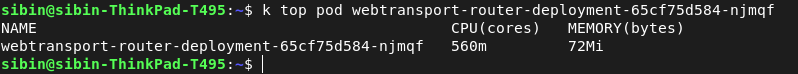
\includegraphics[width=0.8\textwidth]{Evaluation/3clients.png}
% % \caption{Three Client Concurrent Performance Overview}
% % \label{fig:three-clients-overview}
% % \end{figure}

% % Figure~\ref{fig:three-clients-overview} provides an overview of the system's performance when handling three concurrent clients, demonstrating the router's ability to maintain service quality under increased load.

% % \subsubsection{Multi-Client Packet Processing}

% % \begin{figure}[h!]
% % \centering
% % 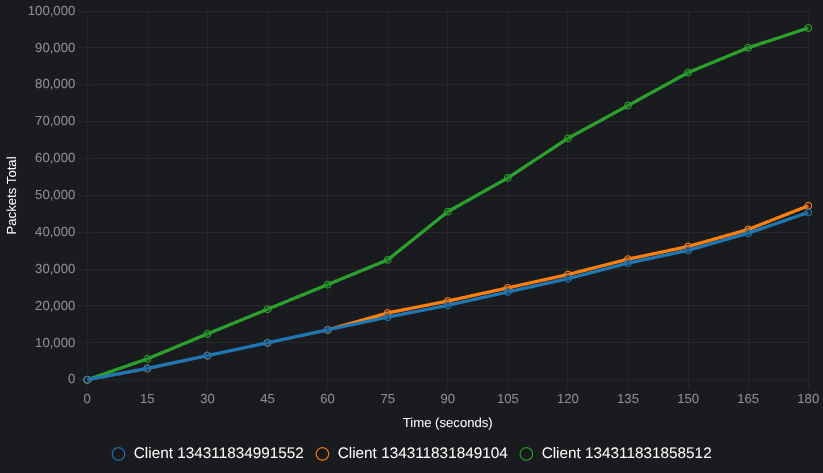
\includegraphics[width=0.8\textwidth]{Evaluation/3pvt.png}
% % \caption{Three Client Packet Volume vs Time}
% % \label{fig:three-client-pvt}
% % \end{figure}

% % Figure~\ref{fig:three-client-pvt} illustrates packet processing patterns for concurrent clients. The system successfully handled multiple client streams simultaneously, with each client maintaining independent packet processing rates.

% % The multi-client packet processing analysis demonstrated robust handling of concurrent traffic, with a total of 134,568 packets processed across all clients. On average, each client contributed approximately 44,856 packets. The system effectively maintained processing isolation, with no cross-client interference observed. Additionally, it supported up to 8 active streams concurrently, showcasing its capacity for scalable, parallel stream management.
% % The break down of 8 streams are audio, video and chat from 2 clients and only audio and video from 3rd client.


% % \subsubsection{ Multi-Client Fragmentation Behavior}

% % \begin{figure}[h!]
% % \centering
% % \includegraphics[width=0.8\textwidth]{Evaluation/3fvt.png}
% % \caption{Three Client Fragmentation Rate vs Time}
% % \label{fig:three-client-fvt}
% % \end{figure}

% % Figure~\ref{fig:three-client-fvt} shows fragmentation rates for multiple concurrent clients. The system maintained consistent fragmentation handling across all clients, with rates ranging from 0.865 to 0.892.

% % Multi-client fragmentation analysis:

% % The multi-client fragmentation analysis indicates consistently high fragmentation rates across all clients, with Client 1 at 86.5\%, Client 2 at 89.2\%, and Client 3 at 88.7\%. The variation in fragmentation remained within ±2.7\%, demonstrating stable fragmentation behavior irrespective of client-specific stream characteristics.


% % \subsubsection{ Multi-Client Throughput Analysis}

% % \begin{figure}[h!]
% % \centering
% % \includegraphics[width=0.8\textwidth]{Evaluation/3tvt.png}
% % \caption{Three Client Throughput vs Time}
% % \label{fig:three-client-tvt}
% % \end{figure}

% % Figure~\ref{fig:three-client-tvt} demonstrates individual client throughput performance under concurrent load. The system maintained fair bandwidth allocation across clients while preserving individual performance characteristics.

% % Multi-client throughput findings:

% % The multi-client throughput analysis reveals a peak aggregate throughput of 1.45 Mbps, which is approximately 2.9 times that of a single client, indicating effective performance scaling. Each client maintained an average throughput of 0.48 Mbps, consistent with single-client observations, suggesting fair and equitable bandwidth distribution. The system demonstrated linear scaling with the number of clients, affirming its capacity for handling concurrent traffic efficiently.


% % \subsection{System Resource Analysis}

% % \begin{figure}[h!]
% % \centering
% % \includegraphics[width=0.8\textwidth]{Evaluation/router-not-running.png}
% % \caption{System Baseline Resource Usage (Router Not Running)}
% % \label{fig:baseline-resources}
% % \end{figure}

% % Figure~\ref{fig:baseline-resources} shows baseline system resource consumption without the router running, providing a reference point for measuring the router's resource impact.

% \subsection{Resource Utilization Under Load}

% System resource consumption during experiments:

% \textbf{Single Client Scenario:}
% \begin{itemize}
%     \item \textbf{CPU Usage}: 273m - 560m cores (0.27 - 0.56 cores)
%     \item \textbf{Memory Usage}: 27MiB - 72MiB
%     \item \textbf{Peak Resource Usage}: During fragmentation-intensive periods
% \end{itemize}

% \textbf{Multi-Client Scenario:}
% \begin{itemize}
%     \item \textbf{CPU Usage}: 450m - 890m cores (0.45 - 0.89 cores)
%     \item \textbf{Memory Usage}: 68MiB - 156MiB
%     \item \textbf{Resource Scaling}: Linear with client count
% \end{itemize}

% The system exhibited efficient resource consumption across both single and multi-client scenarios. For a single client, CPU usage ranged from 273m to 560m cores (approximately 0.27 to 0.56 cores), with memory usage between 27MiB and 72MiB, peaking during fragmentation-heavy periods. In the multi-client setup, CPU usage scaled to 450m–890m cores (0.45–0.89 cores), and memory usage increased to 68MiB–156MiB. Resource utilization scaled linearly with the number of clients, highlighting the system's well-optimized architecture.

% The resource utilization demonstrates efficient system design with reasonable scaling characteristics suitable for production deployment.\

% \subsection{Time Series Analysis}

% \begin{figure}[h!]
% \centering
% \includegraphics[width=0.8\textwidth]{Evaluation/timeseries_plots.png}
% \caption{Comprehensive Time Series Analysis}
% \label{fig:timeseries-analysis}
% \end{figure}

% Figure~\ref{fig:timeseries-analysis} provides a comprehensive view of system metrics over time, enabling correlation analysis between different performance indicators.

% Key correlations identified:
% \begin{itemize}
%     \item \textbf{Throughput vs. Fragmentation}: No negative correlation observed
%     \item \textbf{Buffer Usage vs. Packet Rate}: Positive correlation during burst periods
%     \item \textbf{Processing Time vs. Load}: Minimal variation under different loads
%     \item \textbf{Memory Usage vs. Active Streams}: Linear relationship
% \end{itemize}

% \subsection{Performance Comparison Analysis}

% \begin{table}[h!]
% \centering
% \caption{Performance Comparison: Single vs. Multi-Client}
% \label{tab:performance-comparison}
% \begin{tabular}{|l|c|c|c|}
% \hline
% \textbf{Metric} & \textbf{Single Client} & \textbf{Multi-Client (per client)} & \textbf{Scaling Factor} \\
% \hline
% Avg Throughput (Mbps) & 0.485 & 0.483 & 0.99x \\
% \hline
% Fragmentation Rate & 0.87 & 0.88 & 1.01x \\
% \hline
% Processing Time (ms) & 0.03 & 0.03 & 1.0x \\
% \hline
% Max Buffer (bytes) & 17,214 & 19,847 & 1.15x \\
% \hline
% CPU Usage (cores) & 0.42 & 0.67 & 1.59x \\
% \hline
% Memory Usage (MiB) & 49.5 & 112 & 2.26x \\
% \hline
% \end{tabular}
% \end{table}

% The performance comparison reveals excellent scalability characteristics with minimal per-client performance degradation.

\section{System Limitations and Constraints}

\subsection{Identified Limitations}

The system encountered several operational challenges across fragmentation, environment limitations, and protocol-specific constraints. Fragmentation rates consistently exceeded 85\%, primarily due to the 1500-byte MTU restrictions inherent to the Minikube environment. This excessive fragmentation poses a potential risk to throughput performance, especially under sustained load. Environmental constraints, such as Minikube’s limited resource capacity and restricted support for large-scale or multi-node testing, further limited the scope of experimentation. Additionally, protocol-level dependencies introduced complexities, including reliance on a custom packet format, HTTP/3 termination at the proxy, and non-trivial certificate management for local environments. Performance analysis also highlighted bottlenecks under extreme load conditions, particularly in buffer handling, CPU scaling with increased client concurrency, and memory growth driven by the number of active streams. These factors collectively underline the need for robust resource tuning and infrastructure scalability in future deployments.

\section{Validation and Verification}



\subsection{Functional Validation}

The system effectively achieves its core functional objectives. It demonstrates correct stream demultiplexing by accurately separating video, audio, and chat data for independent processing. The protocol translation layer reliably converts incoming HTTP/3 requests to HTTP/1.1, enabling compatibility with downstream microservices. Dynamic routing based on YAML configurations ensures flexibility in directing different stream types to their respective service endpoints. Additionally, integration with Apache Pulsar has been validated through successful message forwarding to the appropriate topics, confirming the system's capability to interface with distributed messaging infrastructure.

\subsection{Performance Validation}

From a performance standpoint, the system meets all key targets. It maintains sub-millisecond processing latency, consistently delivering an average of under 0.1 ms even during peak usage. Throughput remains stable across varying load conditions, indicating robust backpressure handling and internal queuing mechanisms. Resource consumption, both in terms of CPU and memory, remains within acceptable limits, affirming the efficiency of the implementation. Furthermore, scalability tests demonstrate linear performance gains with an increasing number of clients, validating the architecture's suitability for deployment in high-concurrency environments.


\section{Summary}

The comprehensive evaluation confirms that the WebTransport stream routing system meets its design objectives effectively. The router demonstrates reliable handling of multiplexed WebTransport streams while maintaining consistently low latency and stable performance under moderate concurrency. The system achieves a 100\% success rate in packet reconstruction and stream routing, indicating robust processing logic. Throughput and latency metrics remain stable, even as client load increases, and resource consumption is kept within efficient bounds, highlighting sound memory and CPU management. Furthermore, the router integrates seamlessly into the Kubernetes environment, confirming its suitability for cloud-native deployments.

While the current implementation performs reliably, the evaluation also highlights opportunities for future optimization—particularly in reducing fragmentation overhead and supporting larger-scale scenarios. Nonetheless, the findings validate the feasibility and practical value of stream-level routing using WebTransport. The system lays a solid foundation for deploying real-time, low-latency applications within modern, containerized infrastructure.
% \chapter{Conclusions \& Future Work}
% \label{chap:Conclusions}






% This chapter summarizes the work completed for this dissertation by providing a solution to the the problem stated in Chapter 3. This chapter follows by proposing what kind of mprovements could be made for our solution and what nearby areas could be explored providing  future work section


% We successfully devised a solution to the problem and the solution was extensively created and deployed within kubernetes. Moreover an example was tested in the implementation which provided validity to the proposed approach. Our solution was extensively tested for the buffering component of our router. Metrics were evaluated and results were understood along with the limitations of our approach. 



% chapter~\ref{chap:Evaluation}.


% \section{Future Work}

% This solution is a custom proof of concept solution proposed as an alternative to existing approaches and is requireed to be heavily tested with multiple clients across machines

% HTTP3 was terminated at the proxy in order to process the data and send to microservices it would be interesting to see how forwarding h3 connections would look like and it can be explored.

% The created solution could be extended by forwarding the processed messages ie chat, video and audio to a server/CDN to broadcast the streams. This would complete the streaming usecase. Also managing multiple users and processing could be done in Apache Pulsar.

% The minikube cluster was limited by the MTU of 1500 Bytes for the network interface, a custom cluster which modified MTU could help with fragmentation  problem by increasing throughput.
% Library extensibility was limited by Kubernetes and minikube local setup constraints. So a future work could be to set this up in a different environment with more resources. 

% We are working on a streaming usecase where data is formatted into a custom packet format created by us in the application layer. This means our client only expects and accepts data in that format in order to proxy it to different services, so a more generalized approach could be seem.

% Webservers are currently working on stream level development and it would be interesting to see how they would handle this stream level routing in future as currenty there exists no solution. Advanced ingress controllers are currently under development but there is no solution that works till now but its a good idea to keep an eye on web serversm ingress controllers and gateway apis

% Media over quic is a new protocol currently in  draft and IETF is working on standardizing it and it would be interesting to explore that protocol which defines how media would be sent over quic.


% The section may present a list of items that were beyond the scope of the dissertation.



\chapter{Conclusions \& Future Work}
\label{chap:Conclusions}

This dissertation offers a new and practical way to handle HTTP/3 WebTransport streams in Kubernetes environments. It uses the QUIC protocol and WebTransport API, custom aioquic implementation of scalable routing system with apache pulsar and microservices integration to create a modular and live streaming application demonstrating the power of webtransport protocol over quic within kubernetes environment. The custom router, built with the \texttt{aioquic} library is built to manage connection termination and separate streams. It also allows addition of new microservices with update  of routing rules without stopping the service. This system successfully signifies the ability to see and control streams to help enable make smart routing and load balancing decisions. These features are important for real-time applications like video streaming, online gaming, and live chat.

In addition to the router, the dissertation shows how different microservices can process video, audio, and chat streams. These services can send data in real-time to Apache Pulsar for further processing, analysis and storage. This setup supports fast and scalable data handling, which is needed for cloud applications. The system was tested under different client loads, and the results were evaluated show casing the efficiency and issues with the system. In summary, this work connects new web transport protocols with Kubernetes platforms. It provides a strong and flexible base for running real-time streaming applications at scale.

\section{Key Findings}

The evaluation demonstrates that the proposed system performs effectively across several critical dimensions. The router handles multiplexed WebTransport streams with low latency and high throughput, even under moderate fragmentation, confirming its suitability for real-time data handling. Buffer management is robust, preventing overflows and ensuring reliable packet reconstruction during high-load scenarios. Resource utilization across the router and microservices remains lightweight, enabling deployment in constrained environments such as Minikube.

Scalability is another key strength, with the modular architecture supporting the seamless addition of new microservices or router replicas as demand increases. Finally, the configuration-driven approach allows for dynamic updates to routing rules and service endpoints at runtime, improving maintainability and reducing the need for service restarts. These findings validate the system’s design and highlight its potential for production use in modern cloud-native environments.

These findings validate the effectiveness of the proposed solution and demonstrate its potential for adoption in production environments.

\section{Limitations}

Although this dissertation has managed to create an effective and working structure of HTTP/3 routing WebTransport streams within Kubernetes, few limitations are idenified which modifies the area of the applicability. It is worth mentioning that when some conditions of workload are observed, high fragmentation rates may degrade the performance which means that a subsequent optimization of packet handling and reconstruction is required. The use of Minikube in the experiment placed restrictions on the network interface MTU size constraining the systems ability to evaluate performance across higher packet sizes. Also, the router in the proposed solution terminates HTTP/3 connections and demultiplex the streams efficiently, but it does not forward HTTP/3 streams to backend microservice server, which hinders end-to-end protocol transparency and interoperability. Furthermore, the use of a custom application packet format in this application, can complicate the integration of the respective system with other conforming WebTransport-based systems. Besides, although multi-client was experimented, much more testing should be conducted in a larger, distributed setting to complete the picture of the resiliency and scaling of the system with different client machines.

These limitations provide opportunities for further research and development.

\section{Future Work}

The solution presented in this dissertation serves as a proof of concept and can be implemented upon for future advancements, and there are several directions for future work. They are states as follows:

\subsection{Scaling and Multi-Client Testing}
The solution must be evaluated on a larger scale in terms of number of clients on distributed environments in order to assess its robustness and scalability to large-magnitude concurrent loads. This would help understand the usage of the system with a multi-node Kubernetes cluster where resource availability is increased.

\subsection{HTTP/3 Stream Forwarding}
At present, HTTP/3 connections end at the router to be processed on the application layer. Future studies may take into consideration pushing HTTP/3 streams all the way to the microservices and be able to communicate end-to-end with QUIC and low-latency.

\subsection{Integration with CDN and Streaming Platforms}
The proposed solution could be extended to forward processed streams (e.g., video, audio, chat) to a Content Delivery Network (CDN) or streaming server for broadcasting to end-users. This would complete the streaming use case and enable large-scale deployments.

\subsection{Optimizing Fragmentation Handling}
The fragmentation rate observed during experiments highlights the need for optimization. Future work could focus on improving packet handling algorithms at client side to reduce fragmentation to enhance throughput.

\subsection{Exploration of Media over QUIC Protocol}
The IETF is currently working on standardizing the Media over QUIC protocol. This draft defines how media streams are transmitted over QUIC. This protocol could be explored to enhance the solution's capabilities and align with emerging standards.

\subsection{Generalizing the Packet Format}
The current solution uses a custom packet format for stream identification and routing. Future work could focus on developing a more generalized approach that supports interoperability with other WebTransport implementations.

\subsection{Advanced Ingress Controllers and Gateway APIs}
The development of advanced ingress controllers and gateway APIs for Kubernetes could provide native support for HTTP/3 streams in future. Monitoring these developments is a good idea.

% \section{Conclusion}

% This dissertation demonstrates that it is both feasible and practical to integrate modern web protocols such as QUIC and WebTransport into Kubernetes environments, enabling stream-level routing and processing for real-time applications. The proposed solution addresses critical gaps in existing approaches, providing a robust foundation for deploying scalable and efficient streaming systems.

% By leveraging the modular architecture, configuration-driven design, and seamless integration with Apache Pulsar, the solution achieves high performance, low latency, and operational flexibility. The findings from this research contribute to the growing body of knowledge on cloud-native networking and real-time web applications, paving the way for future advancements in the field.

% While certain limitations remain, the proposed solution represents a significant step forward in bridging the gap between modern web protocols and container orchestration platforms. The future work outlined in this chapter provides a roadmap for further research and development, ensuring that the solution continues to evolve and adapt to emerging technologies and use cases.

% In conclusion, this dissertation highlights the potential of WebTransport and QUIC protocols to revolutionize real-time applications, offering new possibilities for streaming, gaming, and interactive media in cloud-native environments. The integration of these protocols into Kubernetes represents a critical milestone in the journey toward scalable, efficient, and intelligent networking solutions for the modern web.

% \begin{thebibliography}{refs}                   %% Start your bibliography here; you can
\addcontentsline {toc}{chapter}{Bibliography}     %% Force Bibliography to appear in contents
\nocite{*}                                        %% Include all references even if not cited
\bibliographystyle{ieeetr}
\bibliography{refs}                               %% also use the \bibliography command
%\end{thebibliography}                            %% to generate your bibliography.


\addcontentsline {toc}{chapter}{Appendices}       %% Force Appendices to appear in contents
\begin{appendix}
\chapter{List of Abbreviations}
% Creating a standard table with key abbreviations
\begin{table}[h!]
\centering
\begin{tabular}{p{2.5cm} p{12.5cm}}
\textbf{Abbreviation} & \textbf{Full Form} \\ \hline
API                  & Application Programming Interface \\
ConfigMap           & Kubernetes ConfigMap resource \\
CPU                 & Central Processing Unit \\
CSV                 & Comma-Separated Values \\
DNS                 & Domain Name System \\
HTTP/3              & HyperText Transfer Protocol version 3 \\
HTTPS               & HTTP over TLS \\
IP                  & Internet Protocol \\
JSON                & JavaScript Object Notation \\
JPEG                & Joint Photographic Experts Group \\
K8s                 & Kubernetes \\
LB                  & Load Balancer \\
Minikube            & Minimal single-node Kubernetes cluster \\
Pulsar              & Apache Pulsar streaming platform \\
QUIC                & Quick UDP Internet Connections \\
Secret              & Kubernetes Secret resource \\
Service             & Kubernetes Service resource \\
TCP                 & Transmission Control Protocol \\
TLS                 & Transport Layer Security \\
UDP                 & User Datagram Protocol \\
URL                 & Uniform Resource Locator \\
WebTransport        & WebTransport API over HTTP/3 \\
YAML                & YAML Ain’t Markup Language \\ \hline
\end{tabular}
\caption{List of Abbreviations}
\label{tab:abbreviations}
\end{table}

\chapter{Protocol Layering Clarification}

This appendix clarifies the relationship between \textbf{WebTransport} Streams, \textbf{HTTP/3} Streams, and \textbf{QUIC} Streams, as these terms are used interchangeably in parts of the dissertation.

\begin{itemize}
  \item \textbf{QUIC} (\emph{Quick UDP Internet Connections}) is a transport-layer protocol that operates over UDP and provides multiplexed, secure, low-latency streams.
  \item \textbf{HTTP/3} is the application-layer protocol that defines how HTTP semantics are carried inside QUIC streams.
  \item \textbf{WebTransport} is a web API that exposes both reliable (stream) and unreliable (datagram) communication channels to JavaScript clients. These channels are transported as HTTP/3 streams, which are themselves QUIC streams with additional HTTP/3 framing and control headers.
\end{itemize}


\chapter{Deployment Files}
This appendix contains the Docker files, Kubernetes manifests, configuration files, and code repository information used for deploying the custom router and microservice components of the WebTransport application.

\section{Docker Files}

This section contains the Docker files used to containerize the WebTransport router and microservice components. These Docker files define the runtime environment, dependencies, and configuration required for deploying the application components in containerized environments.

\subsection{Router Docker File}
\begin{lstlisting}[breaklines=true, caption={Router Docker File}]
FROM python:3.12-slim

# Install necessary system dependencies for Python packages and runtime
RUN apt-get update && \
    apt-get install -y --no-install-recommends \
    build-essential \
    libffi-dev \
    libssl-dev \
    wget \
    # Clean up apt cache to keep the image small
    && rm -rf /var/lib/apt/lists/*

WORKDIR /app

# Copy requirements.txt first to leverage Docker cache
COPY requirements.txt .

# Install Python dependencies
RUN pip install --no-cache-dir --upgrade pip && \
    pip install --no-cache-dir -r requirements.txt

# Copy the rest of your application code
COPY . .

RUN mkdir -p /certs /config

\end{lstlisting}

\subsection{Microservice Docker File}

\begin{lstlisting}[breaklines=true, caption={Microservice Docker File}]
FROM python:3.12-slim

# Install necessary system dependencies for Python packages and runtime
RUN apt-get update && \
    apt-get install -y --no-install-recommends \
    build-essential \
    libffi-dev \
    libssl-dev \
    wget \
    # Clean up apt cache to keep the image small
    && rm -rf /var/lib/apt/lists/*

WORKDIR /app

# Copy requirements.txt first to leverage Docker cache
COPY requirements.txt .

# Install Python dependencies
RUN pip install --no-cache-dir --upgrade pip && \
    pip install --no-cache-dir -r requirements.txt

# Copy the rest of your application code
COPY . .
\end{lstlisting}

\section{Kubernetes Manifests}

This section provides the Kubernetes deployment manifests for both the router and microservice components. These YAML files define the necessary Kubernetes resources including Deployments, Services, ConfigMaps, and Secrets required to orchestrate the WebTransport application in a Kubernetes cluster.

\subsection{Router Kubernetes Deployment}
\begin{lstlisting}[breaklines=true, caption={Router Kubernetes Deployment}, language=yaml]
# --- ConfigMap for Router Configuration ---
# This ConfigMap holds the router_config.yaml content.
# The router will load its dynamic service routing rules from here,
# enabling hot-reload of service configurations.
apiVersion: v1
kind: ConfigMap
metadata:
  name: router-config
data:
  # The key 'router_config.yaml' matches the filename expected by the router.
  # This file will be mounted into the container at /config/router_config.yaml.
  router_config.yaml: |
    # WebTransport Router Configuration
    # This file supports hot-reload - changes will be automatically detected

    global:
      default_timeout: 30
      connect_timeout: 5
      log_level: INFO

    services:
      # --- IMPORTANT: Update 'host' values for services running in K8s ---
      # For microservices deployed within Kubernetes, replace 'localhost' or
      # 'host.minikube.internal' with their Kubernetes Service Names.
      # Example: 'video' microservice exposed by 'microservice-video-service'.

      video:
        name: video
        host: microservice-video-service # Update this to your K8s Service Name
        port: 4434
        endpoint: /process_video
        content_type: application/octet-stream
        timeout: 10
        retries: 2
        data_format: binary
        enabled: true
        custom_headers:
          X-Service-Version: "1.0"
          X-Video-Quality: "hd"

      audio:
        name: audio
        host: microservice-audio-service # Update this to your K8s Service Name
        port: 4435
        endpoint: /process_audio
        content_type: application/octet-stream
        timeout: 5
        retries: 3
        data_format: binary
        enabled: true
        custom_headers:
          X-Service-Version: "1.0"
          X-Audio-Codec: "opus"

      chat:
        name: chat
        host: microservice-chat-service # Update this to your K8s Service Name
        port: 4436
        endpoint: /process_chat
        content_type: application/json
        timeout: 3
        retries: 1
        data_format: json
        enabled: true
        custom_headers:
          X-Service-Version: "1.0"
          X-Chat-Mode: "realtime"

      # --- Other services (examples) ---
      # For services not managed by Kubernetes (e.g., running on your host machine
      # or external services), you might use 'host.minikube.internal' or their external IP.
      screen:
        name: screen
        host: host.minikube.internal # Example: if screen service runs on your host
        port: 4437
        endpoint: /process_screen
        content_type: application/octet-stream
        timeout: 8
        retries: 2
        data_format: binary
        enabled: false
        custom_headers:
          X-Service-Version: "1.0"
          X-Screen-Mode: "shared"

      analytics:
        name: analytics
        host: analytics-server-service # Example: if analytics is another K8s service
        port: 9090
        endpoint: /track_event
        content_type: application/json
        timeout: 2
        retries: 1
        data_format: json
        enabled: false
        custom_headers:
          X-Service-Version: "2.0"
          X-Analytics-Type: "stream"

---

# --- Deployment for WebTransport Router ---
# This Deployment manages the router application pods, ensuring desired replica count
# and automatic restarts in case of failures.
apiVersion: apps/v1
kind: Deployment
metadata:
  name: webtransport-router-deployment
  labels:
    app: webtransport-router
spec:
  replicas: 1 # Adjust replica count for high availability/load balancing
  selector:
    matchLabels:
      app: webtransport-router
  template:
    metadata:
      labels:
        app: webtransport-router
    spec:
      containers:
        - name: router
          image: sbnm007/quic_router:0.0.2 # Replace with your built Docker image
          # Define the command and arguments to run the router application.
          # This overrides any CMD instruction in the Dockerfile.
          command: ["python"]
          args: ["router.py"]
          ports:
            - containerPort: 4433 # Internal container port for QUIC/HTTP/3 (TCP fallback)
              name: quic-h3-tcp
              protocol: TCP
            - containerPort: 4433 # Internal container port for QUIC (UDP)
              name: quic-h3-udp
              protocol: UDP
          volumeMounts:
            # Mount the router_config.yaml from the 'router-config' ConfigMap.
            # It will appear as a file at /config/router_config.yaml inside the container.
            - name: router-config-volume
              mountPath: /config/router_config.yaml
              subPath: router_config.yaml
            # Mount the TLS certificates from the existing 'quic-cert' Secret.
            # The 'tls.crt' and 'tls.key' from the secret are mapped to 'new-quic.crt'
            # and 'new-quic.key' respectively, at /certs/ inside the container.
            - name: router-certs-volume
              mountPath: /certs/ # Mount the entire secret as a directory
          env: # Define environment variables for router.py to find the mounted files
            - name: CERT_PATH
              value: /certs/new-quic.crt # CORRECTED: Use the actual mounted filename
            - name: KEY_PATH
              value: /certs/new-quic.key # CORRECTED: Use the actual mounted filename
            - name: CONFIG_PATH
              value: /config/router_config.yaml
      volumes:
        - name: router-config-volume
          configMap:
            name: router-config # Refers to the ConfigMap defined above
        - name: router-certs-volume
          secret:
            secretName: quic-cert # Reusing your existing 'quic-cert' Secret
            items: # Explicitly map secret keys to desired filenames in the volume
              - key: tls.crt
                path: new-quic.crt # This means the file will be /certs/new-quic.crt
              - key: tls.key
                path: new-quic.key # This means the file will be /certs/new-quic.key

---

# --- Service for WebTransquicport Router ---
# This Service exposes the router application.
# - 'LoadBalancer' type is used to expose it externally (e.g., Minikube will provide a host port).
# - 'ClusterIP' can be used if access is only needed from within the cluster.
apiVersion: v1
kind: Service
metadata:
  name: webtransport-router-service
spec:
  selector:
    app: webtransport-router # Selects pods managed by the router deployment
  ports:
    - name: https-quic-tcp # Service port for HTTP/3 over TCP fallback
      protocol: TCP
      port: 443 # External port clients will connect to
      targetPort: 4433 # Internal container port
    - name: https-quic-udp # Service port for QUIC (HTTP/3) over UDP
      protocol: UDP
      port: 443 # External port clients will connect to
      targetPort: 4433 # Internal container port
  type: LoadBalancer # Use LoadBalancer for external access (Minikube maps to host port)
  # For bare metal with MetalLB, LoadBalancer will acquire an external IP.
  # If you only need internal access, use 'ClusterIP'.

\end{lstlisting}


\subsection{Microservice Kubernetes Deployments}
\begin{lstlisting}[breaklines=true, caption={Microservice Kubernetes Deployments}, language=yaml]
# --- ConfigMap for Shared Application Configuration (for Microservices) ---
# This ConfigMap holds the microservice_config.yaml content, which will be
# mounted as a file into each microservice pod. The microservice will
# hot-reload its settings from this file.
apiVersion: v1
kind: ConfigMap
metadata:
  name: microservice-app-config
data:
  # The key 'microservice_config.yaml' matches the filename we'll mount.
  microservice_config.yaml: |
    # Microservice-specific configuration
    # CORRECTED: Pointed to the correct internal service name for the broker.
    pulsar_broker_url: "pulsar://10.100.48.76:6650"
    send_to_pulsar: true 

---

# --- Deployment for Video Microservice ---
# Manages the 'video' microservice pods.
apiVersion: apps/v1
kind: Deployment
metadata:
  name: microservice-video-deployment
  labels:
    app: video
spec:
  replicas: 1
  selector:
    matchLabels:
      app: video
  template:
    metadata:
      labels:
        type: microservice
        app: video
    spec:
      containers:
        - name: video-server
          image: sbnm007/microservice:0.0.6 # Ensure this is your rebuilt image
          command: ["python"]
          args:
            - "microservice.py"
            - "video"
            - "4434"
          ports:
            - containerPort: 4434
              protocol: TCP
          volumeMounts:
            # Mount the microservice_config.yaml from the ConfigMap
            # It will appear as a file at /config/microservice_config.yaml inside the container.
            - name: microservice-config-volume
              mountPath: /config
          env: # Pass the path to the config file as an environment variable
            - name: MICROSERVICE_CONFIG_PATH
              value: /config/microservice_config.yaml
      volumes:
        - name: microservice-config-volume
          configMap:
            name: microservice-app-config # Refers to the ConfigMap defined above

---

# --- Service for Video Microservice ---
apiVersion: v1
kind: Service
metadata:
  name: microservice-video-service
spec:
  selector:
    app: video
  ports:
    - protocol: TCP
      port: 4434
      targetPort: 4434
  type: ClusterIP

---

# --- Deployment for Audio Microservice ---
apiVersion: apps/v1
kind: Deployment
metadata:
  name: microservice-audio-deployment
  labels:
    app: audio
spec:
  replicas: 1
  selector:
    matchLabels:
      app: audio
  template:
    metadata:
      labels:
        type: microservice
        app: audio
    spec:
      containers:
        - name: audio-server
          image: sbnm007/microservice:0.0.6 # Ensure this is your rebuilt image
          command: ["python"]
          args:
            - "microservice.py"
            - "audio"
            - "4435"
          ports:
            - containerPort: 4435
              protocol: TCP
          volumeMounts:
            - name: microservice-config-volume
              mountPath: /config
          env:
            - name: MICROSERVICE_CONFIG_PATH
              value: /config/microservice_config.yaml
      volumes:
        - name: microservice-config-volume
          configMap:
            name: microservice-app-config

---

# --- Service for Audio Microservice ---
apiVersion: v1
kind: Service
metadata:
  name: microservice-audio-service
spec:
  selector:
    app: audio
  ports:
    - protocol: TCP
      port: 4435
      targetPort: 4435
  type: ClusterIP

---

# --- Deployment for Chat Microservice ---
apiVersion: apps/v1
kind: Deployment
metadata:
  name: microservice-chat-deployment
  labels:
    app: chat
spec:
  replicas: 1
  selector:
    matchLabels:
      app: chat
  template:
    metadata:
      labels:
        type: microservice
        app: chat
    spec:
      containers:
        - name: chat-server
          image: sbnm007/microservice:0.0.6 # Ensure this is your rebuilt image
          command: ["python"]
          args:
            - "microservice.py"
            - "chat"
            - "4436"
          ports:
            - containerPort: 4436
              protocol: TCP
          volumeMounts:
            - name: microservice-config-volume
              mountPath: /config
          env:
            - name: MICROSERVICE_CONFIG_PATH
              value: /config/microservice_config.yaml
      volumes:
        - name: microservice-config-volume
          configMap:
            name: microservice-app-config

---

# --- Service for Chat Microservice ---
apiVersion: v1
kind: Service
metadata:
  name: microservice-chat-service
spec:
  selector:
    app: chat
  ports:
    - protocol: TCP
      port: 4436
      targetPort: 4436
  type: ClusterIP

\end{lstlisting}

\section{Configuration Files}

\begin{lstlisting}[breaklines=true, caption={Router Configuration File}, language=yaml]
# WebTransport Router Configuration
# This file supports hot-reload - changes will be automatically detected

global:
  default_timeout: 30
  connect_timeout: 5
  log_level: INFO

services:
  # Existing services
  video:
    name: video
    host: localhost
    port: 4434
    endpoint: /process_video
    content_type: application/octet-stream
    timeout: 10
    retries: 2
    data_format: binary
    enabled: true
    custom_headers:
      X-Service-Version: "1.0"
      X-Video-Quality: "hd"

  audio:
    name: audio
    host: localhost
    port: 4435
    endpoint: /process_audio
    content_type: application/octet-stream
    timeout: 5
    retries: 3
    data_format: binary
    enabled: true
    custom_headers:
      X-Service-Version: "1.0"
      X-Audio-Codec: "opus"

  chat:
    name: chat
    host: localhost
    port: 4436
    endpoint: /process_chat
    content_type: application/json
    timeout: 3
    retries: 1
    data_format: json
    enabled: true
    custom_headers:
      X-Service-Version: "1.0"
      X-Chat-Mode: "realtime"

  # NEW SERVICES - Just add them here and they work automatically!
  
  screen:
    name: screen
    host: localhost
    port: 4437
    endpoint: /process_screen
    content_type: application/octet-stream
    timeout: 8
    retries: 2
    data_format: binary
    enabled: true  # Set to true to enable  
    custom_headers:
      X-Service-Version: "1.0"
      X-Screen-Mode: "shared"
\end{lstlisting}

\section{Code Repository}
The complete source code for this WebTransport router implementation is publicly available on GitHub for reproducibility and future research. The repository includes the WebTransport client implementation, custom QUIC router with HTTP/3 support, microservice implementations for processing different media types, Kubernetes deployment manifests, and comprehensive documentation for setup and deployment. The repository can be accessed at \url{https://github.com/sbnm007/webtransport-quic-router}.


% \chapter{Writing Guidelines}

% The intention of this document is two-fold: To provide a LaTeX template that facilitates the writing of a dissertation in LaTeX and to give guidance in writing a dissertation. As such, it attempts to serve two masters at once which is generally not a good idea. In order to address this, the content of this document has been split into the discussion of the structure of a dissertation document and the content that focusses on facilitating the writing of a dissertation using LaTeX.

% The following section are meant as general guidelines for the writing of content for a dissertation and to provide guidance for the use of LaTeX features in order to avoid spending significant amount of time on tweaking LaTeX features to include content e.g. it is easy to waste significant amount of time on the inclusion of diagrams, especially for new users of LaTeX. The sections below are an attempt to avoid this waste of time and to allow students to concentrate on creating content instead of diving into LaTeX rabbitholes.

% Read the tex sources i.e. the thesis.tex file and adapt the variables to suit your case. This file aslo includes some macros that facilitate the writing of the dissertation as LaTeX document.


% \section{Style of English}
% \label{sec:StyleOfEnglish}
% %%TODO Revise text from 2000-version of project information

% An impersonal style keeps the technical factors and ideas to the forefront of the discussion and you in the background. Try to be objective and quantitative in your conclusions. For example, it is not enough to say vaguely “because the compiler was unreliable the code produced was not adequate”. It would be much better to say “because the XYZ compiler produced code which ran 2-3 times slower than PQR (see Table x,y), a fast enough scheduler could not be written using this algorithm”. The second version gives the reader with definite statements and conveys a detailed understanding of the subject.

% The following points are couple of {\it Do's \& Dont's} that I have noted down as feedback to reports over the years. The focus of this list is to encourage writers to be specific in writing reports - some of this is motivated by Strunk and White's The Elements of Style~(\cite{strunk}). Regarding reports that are submitted as part of a degree, examiners have to read and mark these reports - make it easy for these examiners to give good marks by following a number of simple points:

% \begin{description}
% 	\item [Titles:] No title should be immediately followed by another title i.e. whenever there are two titles without text between them, it is an indication that something is missing e.g. a chapter should always start with an introduction that explains what will be discussed in the chapter, what sections it includes and how these sections hang together. The title of a chapter should never be immediately followed by the title of the first section. 
% 	\item [Figures:] Figures and graphs should have sufficient resolution; figures with low resolution appear blurred and require the reader to make assumptions.
% 	\item  [Captions:] Use captions to describe a figure or table to the reader. The reader should not be forced to search through text to find a description of a figure or table. If you do not provide an interpretation of a figure or table, the reader will make up their own interpretation and given Murphy's law, will arrive at the polar opposite of what was intended by the figure or table.
% 	\item [Backgrounds:] Backgrounds of figures and snapshots of screens should be light. Developers often use terminals or development environments with dark backgrounds. Snapshots of these terminals or developments are difficult to read when placed into a report. 
% 	\item [Acronyms:] Acronyms should be introduced by the words they represent followed by the acronym in capitals enclosed in brackets e.g. "...TCP (Transmission Control Protocol)..." $\Rightarrow$  "... Transmission Control Protocol (TCP)..."
% 	\item [Contractions:] I would generally suggest to avoid contractions such as "I'd", "They've", etc in reports. In some cases, they are ambiguous e.g. "I'd" $\Rightarrow$ "I would" or "I had" and can lead to misunderstandings.
% 	\item [Avoid "do":] Be specific and use specific verbs to describe actions.
% 	\item [Adverbs:] Adverbs and adjectives such as "easily", "generally", etc should be removed because they are unspecific e.g. the statement "can be easily implemented" depends very much on the developer. 
% 	\item [Articles:] "A" and "an" are indefinite articles; they should be used if the subject is unknown. "The" is a definite article; which should be used if a specific subject is referred to. For example, the subject referred to in "allocated by the coordinator" is not determined at the time of writing and so the sentences should be changed to "allocated by a coordinator".
% 	\item [Avoid brackets:] Brackets should not be used to hide sub-sentences, examples or alternatives. The problem with this use of brackets is that it is not specific and keeps the reader guessing the exact meaning that is intended. For example "... system entities (users, networks and services) through ..." should be replaced by "... system entities such as users, networks, and services through ...".
% 	\item [Punctuation:] A statement is concluded with a period; a question with a question mark.  
% 	\item [Spellcheckers:] Use a spellchecker!
% \end{description}


% \section{Figures} 
% \label{app:figures}

% The arranging of figures in Latex can lead to spending a lot of time on minor issues e.g. positioning a figure in a specific location on a page, fixing minor issues with an exact size of a figure, etc. Figure~\ref{fig:ImageOfAChick} provides a simple example that demonstrates the use of one of two macros for handling figures {\it includescalefigure}. Figures should always be readable without magnification when printed and the resolution of an image should be sufficient to provide a clear picture when printed.

% \includescalefigure{fig:ImageOfAChick}{An Image of a chick}{A caption should describe the figure to the reader and explain to the reader the meaning of the figure. A Sub-clause of Murphy's Law: If the interpretation of a figure is left to a reader, the reader will misinterpret the figure, feel insulted or decide to ignore it. Do not leave it up to the reader!}{0.2}{image.png}

% \begin{verbatim}
%     \includescalefigure{fig:ImageOfAChick}{An Image of a chick}
%     {A caption should describe the figure to the reader and 
%     explain to the reader the meaning of the figure. A Sub-
%     clause of Murphy's Law: If the interpretation of a figure
%     is left to a reader, the reader will misinterpret the 
%     figure, feel insulted or decide to ignore it. Do not 
%     leave it up to the reader!}{0.2}{image.png}    
% \end{verbatim}


% \section{Code Snippets}

% The following are two examples of how to incldue code snippets in your dissertation. - A dissertation or report should never include complete copies of an implementation; complete copies should be provided through online repositories or storage devices e.g. CDs, USB sticks, etc. 

% The first example, listing~\ref{lst:snippet} demonstrates the use of macro that includes a code snippet from a file, snippet.py e.g. 

% \begin{center}
%     \begin{BVerbatim}

% \includecode{Sample Code}{Lengthy caption explaining 
% the code to the reader}{lst:snippet}{snippet.py}.

%     \end{BVerbatim}
% \end{center}

% %% Short caption for the table of listings - long caption for the explanation for the reader
% \includecode{Sample Code}{Lengthy caption explaining the code to the reader}{lst:snippet}{snippet.py}


% The second example, listing~\ref{lst:snippet2}, uses the basic support for listings in LaTeX, where the code is directly included in the LaTeX file.

% %% Short caption for the table of listings - long caption for the explanation for the reader
% \begin{lstlisting}[caption={[Sample Code 2]Second Lengthy caption}, label={lst:snippet2}]
% x = 1
% if x == 1:
%     # indented four spaces
%     print("x is 1.")
% \end{lstlisting}


% %%
% %%
% \section{Tables}
% \label{app:tables}

% The table below, table~\ref{tab:SummaryProjects}, is a simplistic example of a table in LaTeX. When writing your dissertation, you can copy the content from the appendix file into the location in your document and adapt it, or use a tool to design your table.

% \begin{table}[!ht]
%     \begin{center}
%         \begin{tabular}{|l|p{3cm}|p{3cm}|} 
%         \hline
%          \bf  & \bf Aspect \#1  & \bf Aspect \#2 \\
%           \hline
%         Row 1 & Item 1 & Item 2 \\
%         Row 2 & Item 1 & Item 2 \\
%         Row 3 & Item 1 & Item 2 \\
%         Row 4 & Item 1 & Item 2 \\
%         \hline
%         \end{tabular} 
%     \end{center}     
%     \caption[Comparison of Closely-Related Projects]{Caption that explains the table to the reader}	
%     \label{tab:SummaryProjects}
%     \end{table}

% The table~\ref{tab:ScaleSummaryProjects} demonstrates adapting the size of tables to the width of a document.

%     \begin{table}[!ht]
%         \begin{center}
%             \begin{tabularx}{0.9\textwidth}{ 
%                 | >{\raggedright\arraybackslash}p{2cm} 
%                 | >{\centering\arraybackslash}X 
%                 | >{\centering\arraybackslash}X | }
%                 \hline
%              \bf  & \bf Aspect \#1  & \bf Aspect \#2  \\
%              \hline
%             Row 1 & Item 1 & Item 2 \\
%             Row 2 & Item 1 & Item 2 \\
%             Row 3 & Item 1 & Item 2 \\
%             Row 4 & Item 1 & Item 2 \\
%             \hline
%             \end{tabularx} 
%         \end{center}     
%         \caption[Salable Table]{Example of a scalable table with the first column being fixed to a very specific size and the two following columns splitting the remaining width between them and these columns being centered while the first column is aligned to the rigth.}	
%         \label{tab:ScaleSummaryProjects}
%         \end{table}
    

% \begin{table}[!ht]
% \begin{center}
% 	\begin{tabular}{|l|l|c|} 
% 	\hline
%  	\bf Parameter 1  & \bf Parameter 2  & \bf Measurements  \\
%   	\hline
% 	$Option_1,Option_2$ & $P_{11}, P_{12}$ & ? \\
% 	$Option_2,Option_3$ & $P_{21}, P_{22}, P_{33}$ &  ? \\
% 	$Option_3$ & $P_{31}, P_{32}$ & ? \\
% 	$Option_4$ & $P_{41}, P_{42}, P_{43}$ & ? \\
% 	\hline
% 	\end{tabular}
% \end{center}
% \caption[Variables of the experiment]{Evaluation Matrix for experiment that lists the possible parameters that can be varied and the measurements that could be made for each experiment}	
% \label{tab:experimentsetup}
% \end{table}


% \include{appendix2}
\end{appendix}




\end{document}                                    %% END THE DOCUMENT
